%%%%%%%%%%%%%%%%%%%%%%%%%%%%%%%%%%%%%%%%%
% The Legrand Orange Book
% LaTeX Template
% Version 3.1 (February 18, 2022)
% Compiling this template:
% This template uses biber for its bibliography and makeindex for its index.
% When you first open the template, compile it from the command line with the 
% commands below to make sure your LaTeX distribution is configured correctly:
%
% 1) pdflatex mainv2
% 2) makeindex mainv2.idx -s indexstyle.ist
% 3) biber mainv2
% 4) pdflatex mainv2 x 2


%Atención
%Está prohibido usar simbolos en \index{•} como tildes o simbolos matematicos.
% After this, when you wish to update the bibliography/index use the appropriate
% command above and make sure to compile with pdflatex several times 
% afterwards to propagate your changes to the document.
%
%%%%%%%%%%%%%%%%%%%%%%%%%%%%%%%%%%%%%%%%%

%----------------------------------------------------------------------------------------
%	PACKAGES AND OTHER DOCUMENT CONFIGURATIONS
%----------------------------------------------------------------------------------------

\documentclass[
	12pt, % Default font size, select one of 10pt, 11pt or 12pt
	fleqn, % Left align equations
	a4paper, % Paper size, use either 'a4paper' for A4 size or 'letterpaper' for US letter size
	oneside, % Uncomment for oneside mode, this doesn't start new chapters and parts on odd pages (adding an empty page if required), this mode is more suitable if the book is to be read on a screen instead of printed
]{LegrandOrangeBook}

% Book information for PDF metadata, remove/comment this block if not required 
\hypersetup{
	pdftitle={Telecomunicaciones II}, % Title field
	pdfauthor={Jose Hancco}, % Author field
	pdfsubject={Educación}, % Subject field
	pdfkeywords={Telecomunicaciones, UNSA, Pregrado, Señales}, % Keywords
	pdfcreator={LaTeX}, % Content creator field
}

\addbibresource{sample2.bib} % Bibliography file

\definecolor{ocre}{RGB}{63, 76, 83} % Define the color used for highlighting throughout the book, replace it with average color for a better presentation:
% Background.pdf -> Average color=63,76,83
% Background1.pdf -> Average color=31,31,40
% Background2.pdf -> Average color=123,119,101
% Background3.pdf -> Average color=103,61,76
\chapterimage{Final1.jpg} % Chapter heading image
\chapterspaceabove{6.5cm} % Default whitespace from the top of the page to the chapter title on chapter pages
\chapterspacebelow{6.75cm} % Default amount of vertical whitespace from the top margin to the start of the text on chapter pages

%---------------------------------------------------------------------------------------
\begin{document}

%----------------------------------------------------------------------------------------
%	TITLE PAGE
%----------------------------------------------------------------------------------------

\begingroup
\thispagestyle{empty} % Suppress headers and footers on the title page
\begin{tikzpicture}[remember picture,overlay]
\node[inner sep=0pt] (background) at (current page.center) {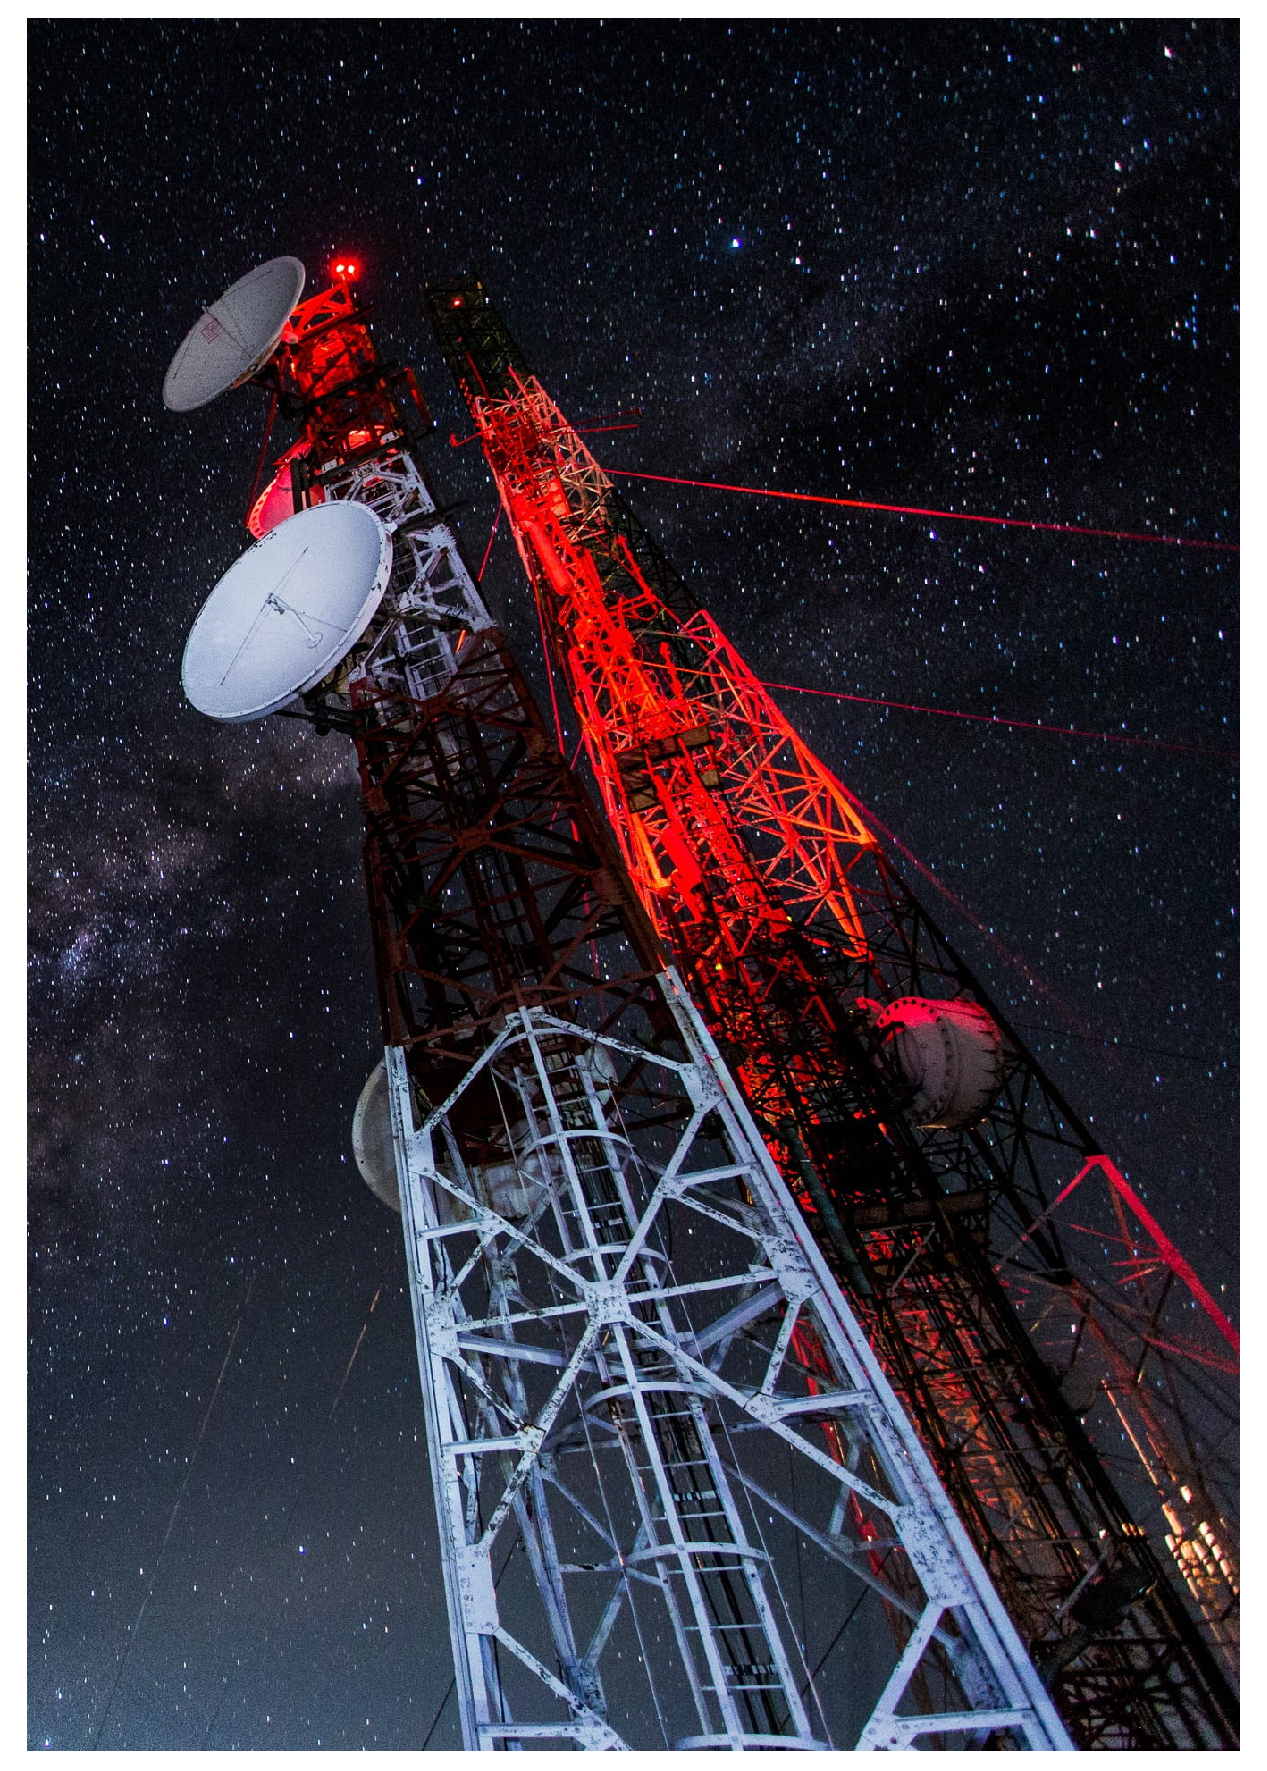
\includegraphics[width=\paperwidth]{background1.pdf}};%here you change your bookcover background
\draw (current page.center) node [fill=ocre!30!white,fill opacity=0.6,text opacity=1,inner sep=1cm]{\Huge\centering\bfseries\sffamily\parbox[c][][t]{\paperwidth}{\centering Telecomunicaciones II\\[15pt] % Book title
{\Large Notas de un estudiante}\\[20pt] % Subtitle
{\huge Jose Antonio Hancco M.}}}; % Author name
\end{tikzpicture}
\vfill
\endgroup

%----------------------------------------------------------------------------------------
%	COPYRIGHT PAGE
%----------------------------------------------------------------------------------------

\newpage
~\vfill
\thispagestyle{empty}

\noindent Copyright \copyright\ 2022 Jose Hancco\\ % Copyright notice

\noindent \textsc{Libro libre de usos}\\ % Publisher

\noindent \textsc{https://github.com/Jose4HM}\\ % URL

\noindent Con licencia de Creative Commons Attribution-NonCommercial 3.0 Unported License (la ``Licencia''). No puede usar este archivo excepto de conformidad con la Licencia. Puede obtener una copia de la Licencia en \url{http://creativecommons.org/licenses/by-nc/3.0}. A menos que lo exija la ley aplicable o se acuerde por escrito, el software distribuido bajo la Licencia se distribuye \textsc{``tal cual'', sin garantías ni condiciones de ningún tipo}, ya sea expresa o implícita. Consulte la Licencia para conocer el idioma específico que rige los permisos y las limitaciones en virtud de la Licencia.\\ % License information, replace this with your own license (if any)

\noindent \textit{Primera edición, septiembre 2022} % Printing/edition date

\noindent Si existe algún error, crees que una sección se puede mejorar o dar cualquier tipo de \textit{feedback} acerca del libro no dudes y mándame un correo a \textit{jhanccoma@unsa.edu.pe}, te responderé lo más pronto que pueda y gracias por mejorar este libro de todos y para todos.
%----------------------------------------------------------------------------------------
%Dedicate
%----------------------------------------------------------------------------------------
\clearpage
\begin{center}
    \thispagestyle{empty}
    \vspace*{\fill}
    \textit{Realmente no sé a quien dedicar este texto, pues no es más que una recopilación de lo que voy aprendiendo para convertirme en ingeniero en telecomunicaciones, visto de manera dedico este libro a todos los estudiantes que por lo menos toman en cuenta la información contenida en el libro y más aún con las ganas de aprender de otro estudiante, como lo soy yo.}
    \vspace*{\fill}
\end{center}
\clearpage
%----------------------------------------------------------------------------------------
%	TABLE OF CONTENTS
%----------------------------------------------------------------------------------------

%\usechapterimagefalse % If you don't want to include a chapter image, use this to toggle images off - it can be enabled later with \usechapterimagetrue

\chapterimage{chapter_head_generalindex3.pdf} % Table of contents heading image

\pagestyle{empty} % Disable headers and footers for the following pages

\tableofcontents % Print the table of contents itself

\cleardoublepage % Forces the first chapter to start on an odd page so it's on the right side of the book

\pagestyle{fancy} % Enable headers and footers again
%----------------------------------------------------------------------------------------
%	PART
%----------------------------------------------------------------------------------------

%----------------------------------------------------------------------------------------
%	NEW CHAPTER
%----------------------------------------------------------------------------------------
\part{Antenas}
\chapterimage{chapter_head_ANT.pdf} % Chapter heading image

\chapter{Conceptos básicos sobre antenas}
\section{Introducción}
Como siempre, antes de este curso hay que recordar algunos términos o conceptos para poder entender cosas que se vienen. Empezamos con las unidades logarítmicas:
\begin{align*}
Belio&=\log\left(\frac{P_{out}}{P_{in}}\right)\\
Decibelio(dB)&=10\cdot\log\left(\frac{P_{out}}{P_{in}}\right)\\
Decibelio(dB)&=20\cdot\log\left(\frac{V_{out}}{V_{in}}\right)\\
Neper(Np)&=ln\left(\frac{V_{out}}{V_{in}}\right)
\end{align*}
Asimismo debemos tener en cuenta las demás medidads respecto a un valor como 1mW, 1W, 1V, etc.\footnote{Estas puedes ser vistas en la sección \textbf{Decibelios} en el capítulo de \textbf{Ingeniería en mantenimiento}.}
Otros conceptos importantes a recordar son:
\begin{definition}[Longitud de Onda]
\begin{equation}
\lambda=\frac{v}{f}
\label{eq:longitud de onda}
\end{equation}
Donde:
\begin{itemize}
\item $\lambda$: Longitud de onda. (m)
\item \textbf{v}: Velocidad. Si el medio es el aire o espacio libre: $v=c=3\times\basedec{8}$ m/s (m/s)
\item $f$: Frecuencia. (Hz)
\end{itemize}
\end{definition}
\begin{definition}[Temperatura]
\begin{equation}
\frac{°C}{5}=\frac{°F-32}{9}=\frac{K-273}{5}=\frac{R-492}{9}
\end{equation}
Despejando podemos obtener:
\begin{align*}
°C=\frac{5}{9}\left(°F-32\right)\\
K=°C+273\\
R=°F+460
\end{align*}
\end{definition}
Además debemos recordar las bandas y frecuencias designadas por la ITU:
\begin{table}[H]
\centering
\begin{tabular}{|c|c|c|c|}
\hline
\rowcolor[HTML]{9698ED} 
N° de banda & Rango de frecuencia & Indicativo & Propagación                    \\ \hline
2           & 30-300 Hz           & ELF        & Onda terrestre                 \\ \hline
3           & 0.3-3 KHz           & SLF        & Onda terrestre                 \\ \hline
4           & 3-30 KHz            & VLF        & Onda terrestre                 \\ \hline
5           & 30-300 KHz          & LF         & Onda terrestre y superficial   \\ \hline
6           & 0.3-3 MHz           & MF         & Onda superficial               \\ \hline
7           & 3-30 MHz            & HF         & Onda superficial y Ionosférica \\ \hline
8           & 30-300 MHz          & VHF        & Onda Ionosférica y directa     \\ \hline
9           & 0.3-3 GHz           & UHF        & Onda directa                   \\ \hline
10          & 3-30 GHz            & SHF        & Onda directa                   \\ \hline
11          & 30-300 GHz          & EHF        & Onda directa e infrarojo       \\ \hline
12          & 0.3-3 THz           &            & Luz infraroja                  \\ \hline
13          & 3-30 THz            &            & Luz infraroja                  \\ \hline
14          & 30-300 THz          &            & Luz infraroja                  \\ \hline
15          & 0.3-3 PHz           &            & Luz visible                    \\ \hline
16          & 3-30 PHz            &            & Luz ultravioleta               \\ \hline
17          & 30-300 PHz          &            & Rayos X                        \\ \hline
18          & 0.3-3 EHz           &            & Rayos X                        \\ \hline
19          & 3-30 EHz            &            & Rayos cósmicos                 \\ \hline
\end{tabular}
\caption{Designación de bandas CCIR por la ITU.}
\end{table}
Los medios de transmisión:
\begin{table}[H]
\resizebox{\textwidth}{!}{
\begin{tabular}{|c|c|c|c|}
\hline
\rowcolor[HTML]{9698ED} 
Medio de transmisión                                                                         & Banda de frecuencia & Longitud de onda & Aplicación principal                                                                                                                                         \\ \hline
\begin{tabular}[c]{@{}c@{}}Par de alambres,\\ cable multipar\end{tabular}                    & 30-300 Hz           & 10000-1000 Km    & Comunicación submarina                                                                                                                                       \\ \hline
\begin{tabular}[c]{@{}c@{}}Par de alambres,\\ cable multipar\end{tabular}                    & 0.3-3 KHz           & 1000-100 Km      & \begin{tabular}[c]{@{}c@{}}Telefonía, transmisión de datos,\\ telex, fax.\end{tabular}                                                                       \\ \hline
\begin{tabular}[c]{@{}c@{}}Par de alambres,\\ cable multipar,\\ ondas de tierra\end{tabular} & 3-30 KHz            & 100-10 Km        & \begin{tabular}[c]{@{}c@{}}Telefonía de onda portadora baja,\\ capacidad, navegación y radiotelegrafía.\end{tabular}                                         \\ \hline
\begin{tabular}[c]{@{}c@{}}Par de alambres,\\ ondas de tierra\end{tabular}                   & 30-300 KHz          & 10-1 Km          & \begin{tabular}[c]{@{}c@{}}Telefonía de onda portadora mediana\\ capacidad, radiofaro, navegación,\\ radiodifusión onda larga.\end{tabular}                  \\ \hline
\begin{tabular}[c]{@{}c@{}}Cable coaxial, ondas\\ de cielo\end{tabular}                      & 0.3-3 MHz           & 1000-100 m       & \begin{tabular}[c]{@{}c@{}}Radiodifusión, AM, radio aficionados,\\ radio móvil.\end{tabular}                                                                 \\ \hline
\begin{tabular}[c]{@{}c@{}}Cable coaxial, cable UTP cat 3-4,\\ ondas de cielo\end{tabular}   & 3-30 MHz            & 100-10m          & \begin{tabular}[c]{@{}c@{}}Radio aficionados, comunicaciones milirares,\\ marítimas, radio telefonía movil.\end{tabular}                                     \\ \hline
\begin{tabular}[c]{@{}c@{}}Cable coaxial, cable UTP cat 5,\\ ondas directas\end{tabular}     & 30-300 MHz          & 10-1 m           & \begin{tabular}[c]{@{}c@{}}TV, radiodifusión FM, multiacceso radial,\\ radio enlaces, direccionales.\end{tabular}                                            \\ \hline
Ondas directas                                                                               & 0.3-3 GHz           & 100-10 cm        & \begin{tabular}[c]{@{}c@{}}TV, telemetría por radar, comunicaiones\\ militares por satélite, telefonía celular, radio\\ de espectro ensanchado.\end{tabular} \\ \hline
Guía de onda, línea visual                                                                   & 3-30 GHz            & 10-1 cm          & \begin{tabular}[c]{@{}c@{}}Comunicaiones vía satélite, radio enlace\\ direccional analógico y digítal, operación\\ aérea por radar.\end{tabular}             \\ \hline
Guía de onda, línea visual.                                                                  & 30-300 GHz          & 1-0.1 cm         & \begin{tabular}[c]{@{}c@{}}Comunicación militar por satelite, \\ radio astronomia, aterrizaje por radar.\end{tabular}                                        \\ \hline
Fibra óptica                                                                                 & 100-1000 THz        & 3-0.3 pm         & \begin{tabular}[c]{@{}c@{}}Telefonia muy alta capacidad, servicios de\\ banda ancha (SONET, SDH y ATM),\\ video conferencia, CATV por F.O.\end{tabular}      \\ \hline
\end{tabular}
}
\end{table}
\subsection{Ancho de banda y capacidad de información}\index{Ancho de banda y capacidad de información}
Las limitaciones más importantes para el funcionamiento de una sistema de comunicaciones son el \textbf{ruido} y el \textbf{ancho de banda}. El ancho de banda de un canal de comunicación es la diferencia entre la frecuencia máxima y mínima que puede pasar por el canal. El ancho de banda de un canal de comunicación debe ser igual o mayor que el ancho de banda de la información.
\begin{definition}[Ley de Hartley]
Es la medida de cuanta información se puede transferir a través de un sistema de comunicaciones en un determinado tiempo.
\begin{equation}
I\approx B\times t
\label{eq:hartley}
\end{equation}
Donde:
\begin{itemize}
\item \textbf{I}: Capacidad de información.
\item \textbf{B}: Ancho de banda. (Hz)
\item \textbf{t}: Tiempo de transmisión. (s)
\end{itemize}
\end{definition}
\begin{notation}
Se requieren \textbf{3 KHz} de ancho de banda para transmitir las señales telefónicas con calidad de voz.\\
Se asigna \textbf{200 KHz} para transmisión comercial de FM para música, con alta fidelidad.\\
Se requieren casi \textbf{6 MHz} de ancho de banda para emitir señales de televisión de alta calidad
\end{notation}
Otra medida que debemos saber es:
\begin{definition}[Capacidad de información de un canal digital]
Shannon relacionó la capacidad de información de un canal de comunicaciones, en bits por segundo (bps), con el ancho de banda y la relación señal a ruido: 
\begin{equation}
I=B\cdot\log_2(1+S/N)
\label{eq:shannon}
\end{equation}
Donde:
\begin{itemize}
\item I: Capacidad de información. (bps)
\item B: Ancho de banda. (Hz)
\item S/N: Relación señal a ruido.
\end{itemize}
\end{definition}
\subsection{Ruido}\index{Ruido}
Energía eléctrica \textbf{no deseable} presente en la banda útil del circuito de comunicación. Se puede clasificar el ruido en dos categorías:
\begin{enumerate}
\item \textbf{Correlacionado}: Solo existe \textbf{cuando hay una señal}. Es aquel que se relaciona mutuamente con la señal, y no puede estar en un circuito a menos que haya una señal de entrada.
Se produce por amplificación no lineal, e incluye la distorsión armónica (cuando se producen las armónicas no deseadas de una señal, debido a una amplificación no lineal) y de intermodulación (generación de frecuencias indeseables de suma o diferencia), ya que las dos son formas de distorsión no lineal.
\item \textbf{No Correlacionado}: Está presente \textbf{siempre}, haya o no señal. El ruido no correlacionado puede sub dividirse en dos categorías generales:
\begin{enumerate}
\item \textbf{El Ruido Externo }es el que se genera fuera del dispositivo o circuito. Hay tres causas principales de ruido Externo:
\begin{enumerate}
\item \textbf{Ruido atmosférico}: Perturbaciones eléctricas naturales. Electricidad estática (rayos)
\item \textbf{Ruido extraterrestre}: Señales eléctricas originadas fuera de la atmósfera terrestre (solar y cósmico)
\item \textbf{Ruido hecho por el hombre}: Su puente principal son mecanismos que producen chispas, ruido industrial (conmutadores, generadores, lámparas fluorescentes)
\end{enumerate}
\item \textbf{El Ruido Interno} es la interferencia eléctrica generada dentro de un dispositivo o circuito. Las causas principales son:
\begin{enumerate}
\item \textbf{Ruido Térmico}: Asociado con el movimiento rápido y aleatorio de electrones libre, producido por la agitación térmica.
\item \textbf{Ruido de Tiempo de Tránsito}: Variación irregular y aleatoria, producida por la modificación de una corriente de portadores, cuando pasa de la entrada a la salida de un dispositivo.
\item \textbf{Ruido de Disparo}: Se debe a la llegada aleatoria de portadoras al elemento de salida de un dispositivo electrónico (diodo, FET, transistor bipolar).
\end{enumerate}
\end{enumerate}
\end{enumerate}
\subsection{Ruido térmico}\index{Ruido térmico}
Es el movimiento \textbf{aleatorio} de los electrones libres dentro de un conductor, causado por la agitación térmica. Lamentablemente, este ruido está a lo largo de todo el espectro electromagnético.
Llamado también: Movimiento Browniano por su descubridor Robert Brown, Ruido de Johnson en honor a quien lo relacionó con el movimiento de los electrones y Ruido Blanco porque se produce en todas las frecuencias.
\begin{definition}[Potencia de ruido térmico]
\begin{equation}
P_{tn}=K\cdot T\cdot B
\label{eq:ruido termico}
\end{equation}
Donde:
\begin{itemize}
\item $P_{tn}$: Potencia del ruido  térmico\footnote{tn:thermal noise o ruido térmico.} (W)
\item \textbf{K:} Constante de Boltzmann= $1.38\times\basedec{-23} J/°K$.
\item \textbf{T}: Temperatura absoluta. (°K)
\item \textbf{B}: Ancho de banda. (Hz)
\end{itemize}
Alternativamente, el ruido térmico puede ser expresado en dBm, para ello debemos usar la siguiente expresión comparada con un 1mW:
\begin{equation}
P_{tn}(dBm)=10\cdot\log\left(\frac{K\cdot T\cdot B}{0.001}\right)
\label{eq:ruido termico log}
\end{equation}
En temperatura ambiente (17 C o 290 K), el ruido térmico ambiente:
\begin{equation}
P_{tn}(dBm)=-174 dBm+10\log(B)
\label{eq:ruido termico ambiente}
\end{equation}
\end{definition}
\begin{definition}[Voltaje ruido térmico]
\begin{equation}
V_{tn}=\sqrt{4\cdot R\cdot K\cdot T\cdot B}
\label{eq:voltaje ruido termico}
\end{equation}
Donde:
\begin{itemize}
\item \textbf{R}: Resistencia interna. ($\Omega$)
\item \textbf{$V_{tn}$}: Voltaje RMS del ruido. (V)
\end{itemize}
\end{definition}
\begin{notation}
Para la máxima potencia transferencia de potencia $R_L=R_I$.
\end{notation}
\begin{definition}[Relación señal a ruido-SNR]
Es la relación en decibelios entre la potencia de la señal(S) y la potencia del ruido(N):
\begin{equation}
\label{eq:snr}
SNR=10\log_{10}\left(\frac{S}{N}\right)=20\log_{10}\left(\frac{V_s}{V_n}\right)
\end{equation}
\end{definition}
\begin{remark}
El \textbf{factor a ruido} se define como el cociente entre la potencia SNR de entrada y potencia SNR de salida. Por consecuencia, la \textbf{cifra de ruido} es el factor de ruido expresado en dB.
\end{remark}
\begin{notation}
Para voltaje, 6dB indica que la salida es dos veces el valor de la entrada, es decir: Si la entrada es 1, la salida será 2. Para potencia, 3dB indica lo mismo: el valor de la salida es dos veces el valor de la entrada.
\end{notation}
\subsection{Ángulo crítico}\index{Angulo crítico}
Debemos recordar ecuaciones como Ley de Snell,
\begin{definition}[Ley de Snell]
\begin{align}
n_1\sin\theta_1&=n_2\sin\theta_2\\
\sqrt{\epsilon_1}\sin\theta_1&=\sqrt{\epsilon_2}\sin\theta_2
\label{eq:snell}
\end{align}
Donde:
\begin{itemize}
\item $n$: Indice ión.
\item $\theta$ Ángulo de refracción.
\item $\epsilon$: Permitividad relativa del material.
\end{itemize}
\end{definition}
\begin{figure}[H]
\centering
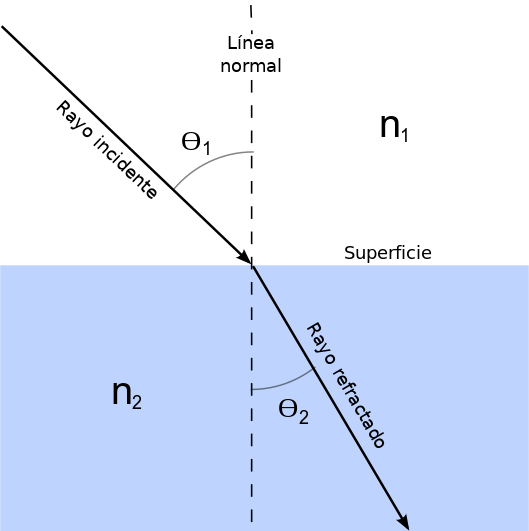
\includegraphics[width=0.6\linewidth]{Ant/Ant6.png}
\caption{Ley de Snell}
\end{figure}
dentro de ella una que usaremos es la del \textit{ángulo crítico}:
\begin{center}
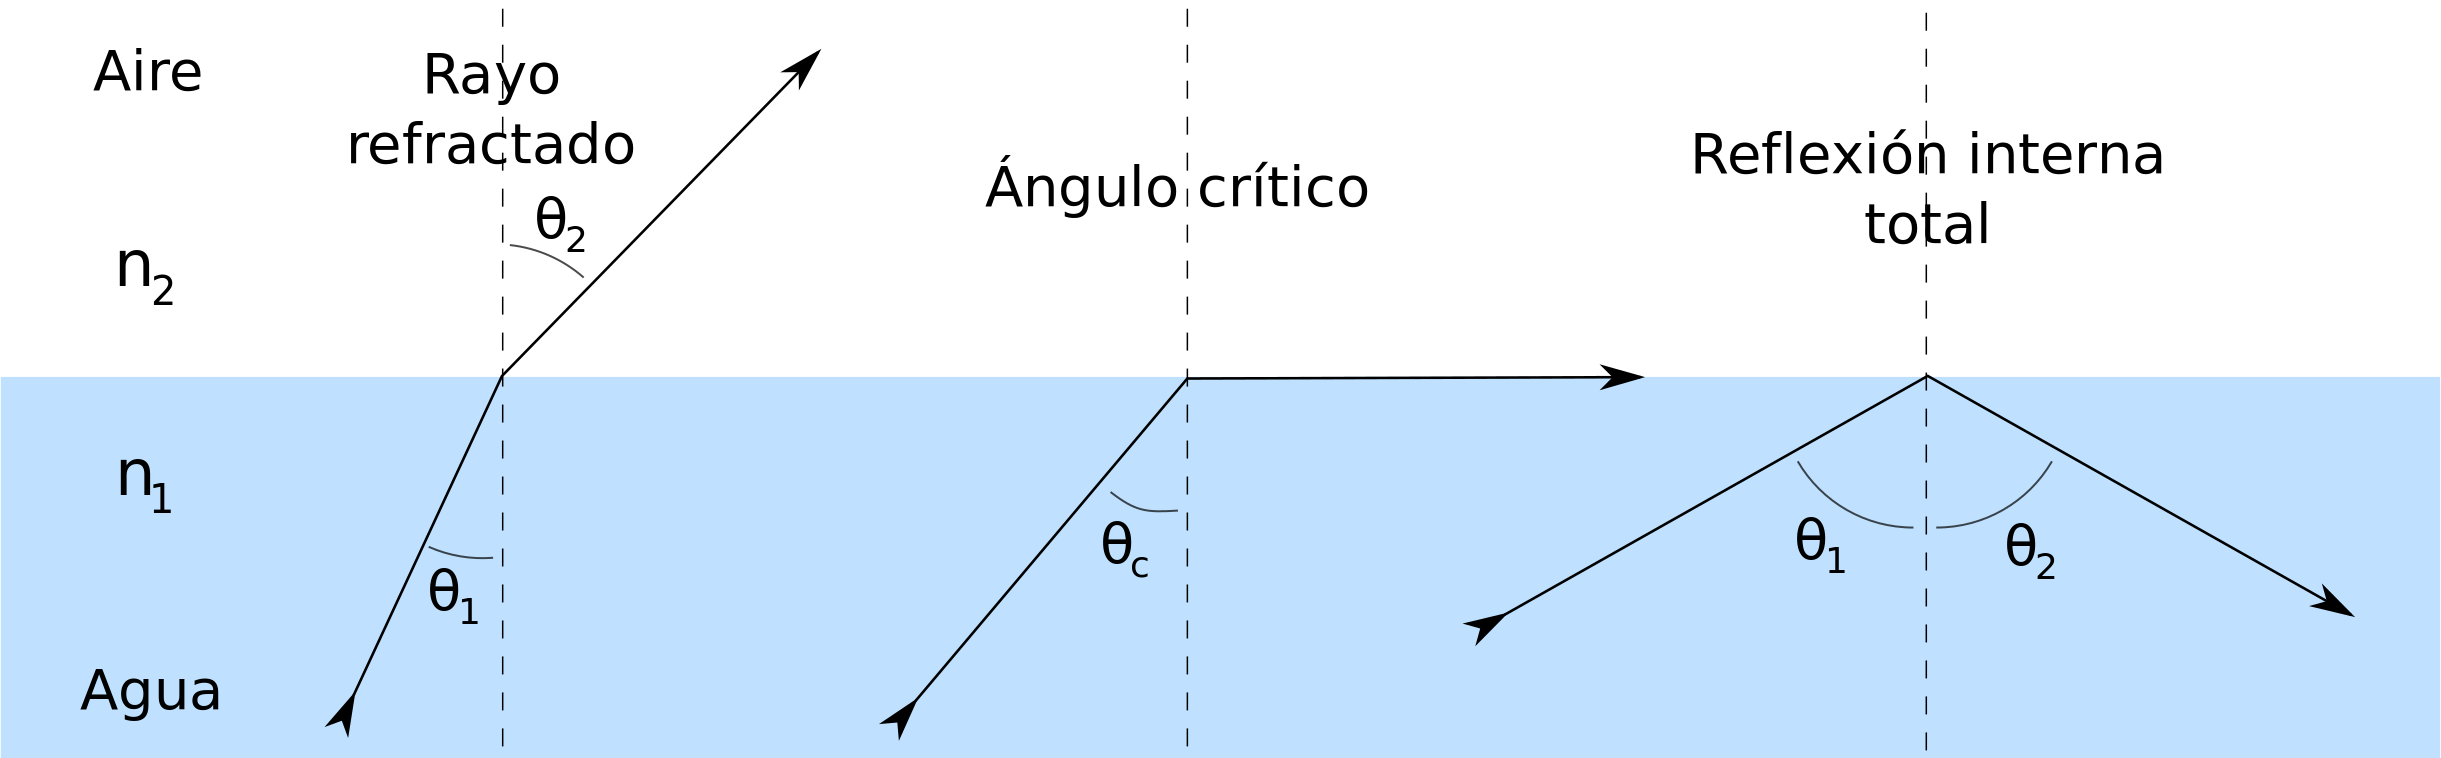
\includegraphics[width=0.8\linewidth]{Ant/Ant1.png}
\end{center}
La forma de obtener el ángulo crítico es:
\begin{equation}
\sin\theta_c=\frac{n_2}{n_1}
\label{eq: angulo critico}
\end{equation}
\begin{notation}
El índice de refracción esta definido como el cociente de la \textbf{velocidad de la luz en el vacío} entre la \textbf{velocidad de la luz del medio donde se propaga}. Generalmente se utiliza la velocidad de la luz en el vacío (\textit{c}) como medio de referencia para cualquier materia, aunque durante la historia se han utilizado otras referencias, como la velocidad de la luz en el aire. En el caso de la luz, es igual a $n=\sqrt{\epsilon_r\cdot\mu_r}$. Para la mayoría de los materiales, la \textbf{permeabilidad magnética relativa} ($\mu_r$) es muy cercano a 1 en frecuencias ópticas, es decir, luz visible, por lo tanto, \textit{n} es aproximadamente $\sqrt{\epsilon_r}$
\end{notation}
\subsection{Repaso: Propagación de ondas electromagnéticas}
La propagación de OEM por el espacio libre se suele llamar propagación de radiofrecuencia o radio propagación. Las OEM, en el espacio libre se propagan en línea recta a la velocidad de la luz ($3\basedec{8}m/s$). 
\begin{definition}[Distancia máxima de línea]
\begin{subequations}
\begin{align}
d_{max}&=\sqrt{2\cdot h}
\label{eq:dist millas} \\
d_{max}&=\sqrt{17\cdot h}\label{eq:dist km}
\end{align}
\end{subequations}
Donde:
\begin{itemize}
\item $d_{max}$: Distancia máxima de línea de vista. (millas ó Km)
\item \textbf{h}: Altura (Pies ó m)\footnote{La distancia será en millas si se trabaja con la ecuación \ref{eq:dist millas}, donde la altura debe ser introducida en pies. Para la ecuación \ref{eq:dist km}, la distancia estará en metros y la altura en metros.}
\end{itemize}
\end{definition}
Hablemos también de las \textbf{pérdidas por trayectoria}. El modelo de pérdida por trayectoria en el espacio libre es usado para predecir la intensidad del nivel de recepción cuando el transmisor y receptor tienen una trayectoria de línea de vista clara, sin obstrucciones entre ellos.
\begin{definition}[Pérdidas por trayectoria]
\begin{subequations}
\begin{align}
&L_p=\left(\frac{4\pi\cdot d}{\lambda}\right)^2=\left(\frac{4\pi\cdot d\cdot f}{c}\right)^2
\label{eq:perdidas trayec adimensional} \\
&L_p=20\cdot\log\left(\frac{4\pi\cdot d\cdot f}{c}\right)=20\cdot\log\left(\frac{4\pi}{c}\right)+20\cdot\log(f)+20\cdot\log(d)\label{eq:perdidas trayec db}
\end{align}
\end{subequations}
Donde:
\begin{itemize}
\item \textbf{d}: Distancia. (m)
\item \textbf{\textit{f}}: Frecuencia. (Hz)
\item \textbf{\textit{c}}: Velocidad de la luz.
\item $\lambda$: Longitud de onda. (m)
\end{itemize}
Si la distancia se expresa en Km y la frecuencia en MHz:
\begin{equation}
L_p(dB)=32.4+20\cdot\log(f)+20\log(d)
\end{equation}
\end{definition}
Otro término usado es la \textbf{polarización}, recordando que una OEM contiene un campo eléctrico y un campo magnético que forman 90° entre sí. Por lo tanto, la polarización de una OEM plana, no es mas que la orientación del vector campo eléctrico respecto a la superficie de la tierra.\\
\textbf{Tipos de polarización:}
\begin{enumerate}
\item \textbf{Polarización lineal}: Si la polarización permanece constante. Las formas lineales son:(Fig. \ref{fig:pol lin})
\begin{enumerate}
\item \textbf{Polarización Horizontal}: Campo eléctrico paralelo a la superficie de la tierra.
\item \textbf{Polarización Vertical}: Campo eléctrico perpendicular a la superficie terrestre.
\end{enumerate}
\item \textbf{Polarización Circular}: Luz polarizada circularmente consta de dos ondas electromagnéticas planas perpendiculares con una diferencia de fase de 90º. (Fig. \ref{fig:pol circ})
\item \textbf{Polarización elíptica}: La luz polarizada elípticamente consiste de dos ondas perpendiculares de amplitudes desiguales y con una diferencia de fase de 90º. (Fig. \ref{fig:pol elip})
\end{enumerate}
\begin{figure}[]
\centering
\subfloat[El campo eléctrico transversal de la onda va acompañado de un campo magnético como el que se ilustra.]{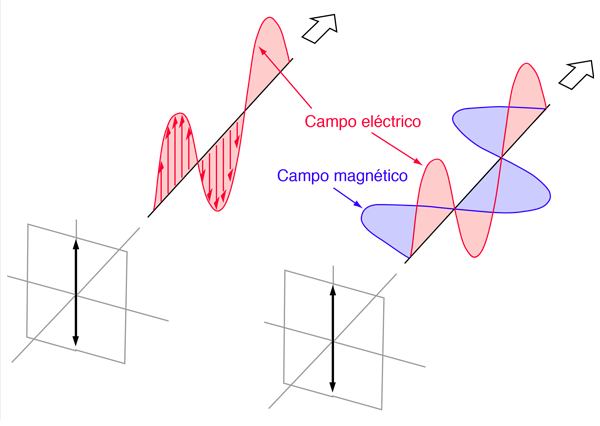
\includegraphics[width=0.5\linewidth]{Ant/Ant2.png}
\label{fig:pol lin}}
\subfloat[El vector de polarización gira 360º a medida de que la onda recorre una longitud de onda en el espacio]{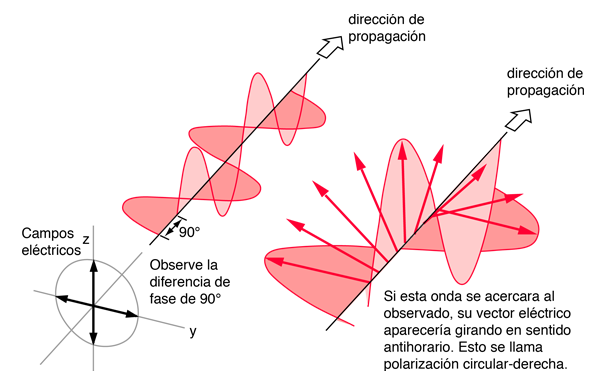
\includegraphics[width=0.5\linewidth]{Ant/Ant3.png}\label{fig:pol circ}}\\
\subfloat[Cuando la Intensidad de Campo varía con cambios en la polarización, se dice que es una Polarización Elíptica.]{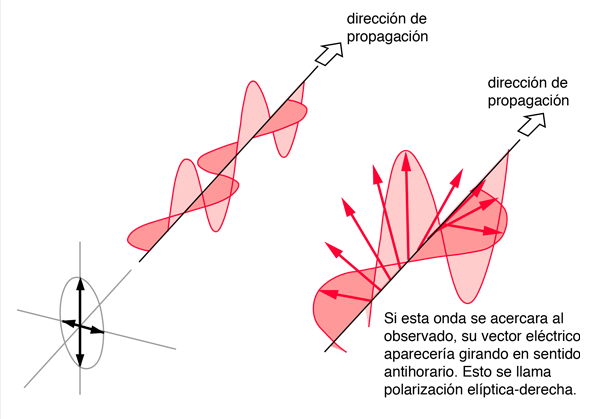
\includegraphics[width=0.5\linewidth]{Ant/Ant4.png}\label{fig:pol elip}}
\subfloat[Tipos de polarizaciones.]{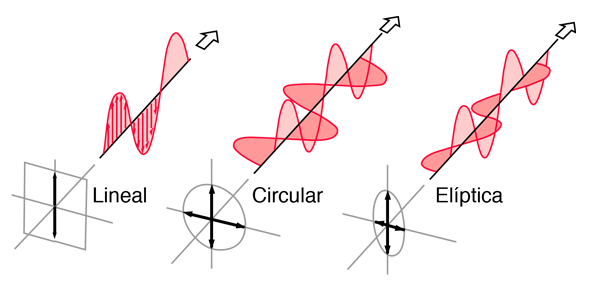
\includegraphics[width=0.5\linewidth]{Ant/Ant5.png}}
\caption{Polarización de ondas.}
\end{figure}
\begin{notation}
Si el vector gira en sentido de las manecillas del reloj, se dice que es Derecho, si es contrario se dice que es Izquierdo
\end{notation}
\subsubsection{Densidad de potencia radiada}
La \textbf{rapidez} con que la energía pasa a través de una \textbf{superficie} dada en el espacio libre se llama D\textbf{ensidad de Potencia}. La \textbf{Densidad de Potencia Radiada} se define como la potencia por unidad de superficie en una determinada dirección. Las unidades son \textbf{Watt por Metro Cuadrado} ($W/m^2$). Se puede calcular a partir de los valores eficaces de los campos eléctrico o magnéticos.
\begin{definition}[Potencia Isotrópica Radiada Equivalente]
\begin{equation}
PIRE=P_r\cdot D=P_A\cdot G
\label{eq:pire}
\end{equation}
Donde:
\begin{itemize}
\item PIRE:  Potencia Isotrópica Radiada Equivalente. (W)
\item $P_R$: Potencia de radiación.
\item $P_A$: Potencia suministrada a la antena. (W)
\item \textbf{G}: Ganancia.
\item \textbf{D}: Directividad de la antena.\footnote{Estos conceptos se detallan más adelante.}
\end{itemize}
\end{definition}
\begin{definition}[Densidad de potencia]
Es la intensidad de los campos eléctrico y magnético de una onda electromagnética que se propaga por el espacio libre.
\begin{equation}
\mathbb{P}=E\cdot H=\frac{PIRE}{4\pi r^2}=Z_s\times H^2=\frac{E^2}{Z_s}
\label{eq:int campo}
\end{equation}
Donde:
\begin{itemize}
\item $\mathbb{P}$: Densidad de potencia. ($W/m^2$)
\item \textbf{E}: Intensidad de campo eléctrico. (V/m)
\item \textbf{H}: Intensidad del campo magnético. (A/m)
\item \textbf{r}: Radio de la esfera. (m)
\item \textbf{\textit{PIRE}}: Potencia Isotrópica Radiada Equivalente. (W)
\item \textbf{$Z_S$}: Impedancia en el vacío. ($\Omega$)
\end{itemize}

\end{definition}
\begin{definition}[Impedancia en el espacio libre]
La relación entre el módulo del campo eléctrico y el módulo del campo magnético es la impedancia característica del medio. La impedancia característica de un medio de transmisión \textbf{sin pérdidas} en igual a la raíz cuadrada de la relación de su permeabilidad magnética entre su permitividad eléctrica:
\begin{equation}
Z_s=\sqrt{\frac{\mu_0}{\epsilon_0}}=377\Omega
\label{eq:imp carac espacio libre}
\end{equation}
Donde:
\begin{itemize}
\item $Z_s$: Impedancia en el espacio libre. ($\Omega$)
\item $\mu_0$: Permeabilidad magnética ($1.26\basedec{-6}$H/m ó $4\pi\cdot K N/A^2$ donde $K=\basedec{-7}$).
\item $\epsilon_0$: Permitividad eléctrica del vacío ($8.85\basedec{-12}$F/m).
\end{itemize}
\end{definition}
%\begin{definition}[Potencia total radiada]
%Se puede obtener como la integral de la Densidad de Potencia en una esfera que encierre a la antena.
%\begin{equation}
%P_{tr}=\frac{P_{rad}}{4\pi r^2}
%\end{equation}
%\end{definition}
La \textbf{Intensidad de Radiación} es la potencia radiada por unidad de ángulo sólido en una determinada dirección.
\subsubsection{Ley de cuadrado inverso}
La \textbf{densidad de potencia} es inversamente proporcional al cuadrado de la distancia de la fuente.
\begin{equation}
\frac{\mathbb{P}_2}{\mathbb{P}_1}=\left(\frac{r_1}{r_2}\right)^2
\label{eq:ley cuadrado inverso}
\end{equation}
Para que se cumpla esta ley, la velocidad de propagación en todas las direcciones debe ser uniforme (Medio Isotrópico)
\subsubsection*{Atenuación y absorción}
\textbf{Atenuación} es la reducción de la Densidad de Potencia con la distancia. La atenuación se debe al esparcimiento esférico de la onda, se le llama ``atenuación espacial'' de la onda. Se expresa generalmente en términos del logaritmo de la relación de  densidad de  potencia (pérdida en dB)\\
\textbf{Absorción} solo se presenta cuando los CEM se propagan por la atmósfera. Es la energía transferida de la OEM a los átomos y las moléculas de la atmósfera. La absorción de radiofrecuencias en una atmósfera normal, es relativamente insignificante a frecuencias por debajo de 10 GHz.
\section{Antenas}
Las dos funciones primordiales de la antena son:
\begin{enumerate}
\item Convertir la energía electromagnética, procedente del generados a través de la línea de transmisión, en energía electromagnética que se propaga libremente por el espacio.
\item Adapta la impedancia interna del generador a la impedancia del espacio.
\end{enumerate}
En las líneas de transmisión se propagan ondas electromagnéticas \textbf{guiadas}, es decir campos electromagnéticos variables entre cargas y corrientes. Las antenas convierten estos ondas electromagnéticas guiadas en \textbf{libres} y \textbf{viceversa}. Tanto las ondas guiada como las libres son señales de radio.\\
En el proceso de su propagación, las ondas de radio se \textbf{dispersan} más allá de las líneas de radio-comunicación y son absorbidas por el medio circundante. Si la dirección de radiocomunicación es conocida y limitada, las perdidas pueden reducirse concentrando las ondas emitidas en direcciones definidas.\\
Con lo definido sobre antenas y conocimientos en impedancias, podemos definir:
\begin{corollary}[Impedancia de antena]
Es la relación entre tensión y corriente en sus terminales de entrada (de la antena). Como todas, dicha impedancia es en general compleja: parte real ó resistencia de antena y la parte compleja ó reactancia de antena.
\end{corollary}
\subsection{Tipos de antenas}
A grandes rasgos existen dos tipos de antenas: antenas de \textbf{transmisión} y antenas de \textbf{recepción}.
\subsubsection*{Antenas de transmisión}
La antena de transmisión transforma energía de un campo electromagnético estacionario producido por la señal de radio, en energía de un campo electromagnético de radiación, añadiendo además que este último debe emitirse en unas direcciones dadas.
\begin{figure}[]
\centering
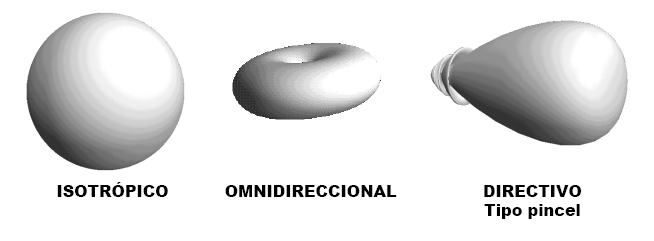
\includegraphics[width=0.8\linewidth]{Ant/Ant7.png}
\caption{Gráficas de antena.}
\end{figure}
\subsubsection*{Antenas de recepción}
La antena de recepción está destinada a la transformación de la energía de una radioseñal consistente en un campo de radiación que procede de una dirección dada, en energía de un campo estacionario de ondas electromagnéticas.
\begin{remark}
La antena de transmisión y recepción tienen procesos \textbf{recíprocos}. Esto quiere decir que existe la posibilidad de utilizar la misma antena en calidad de transmisora y de receptora, y de conservar invariables los parámetros principales de la antena.
\end{remark}
\subsection{Características y parámetros de las antenas transmisoras}
Los parámetros de una antena son los que permiten especificar el funcionamiento de las mismas, y por lo tanto son susceptibles de ser medidos. Se puede especificar la antena como un \textbf{conjunto de parámetros} conectados con los  requisitos de un sistema más amplio de radiocomunicaciones o radiodifusión.\\
\textbf{Parámetros de antena}:
\begin{itemize}
\item Diagrama de radiación
\item Densidad de potencia radiada
\item \textbf{Directividad}: Es la relación entre la densidad de potencia radiada en la dirección de máxima radiación, a una cierta distancia R, y la potencia total radiada dividida por el área de la esfera de radio R. La directividad se puede calcular a partir del diagrama de radiación. La ganancia de una antena es igual a la directividad multiplicada por la eficiencia. La relación entre la densidad de potencia radiada por la antena en la dirección útil y la que radia por el lóbulo trasero se conoce como relación delante/detrás (forward/backward) y es un importante parámetro de diseño de la antena en lo relativo a interferencias.\\
El ángulo que hace referencia al diagrama de radiación del lóbulo principal en el planohorizontal de la antena se denomina ``azimut'', que para el diagrama de radiación vertical se denomina ``ángulo de elevación'', que se diseña para concentrar el máximo de radiación para aquellos ángulos por debajo de la horizontal, que es donde se agrupan los usuarios, ya que las antenas se colocan en cotas elevadas para alcanzar una mayor cobertura.
\item \textbf{Ganancia}: Es la relación entre la densidad de potencia radiada en la dirección del máximo a una distancia R y la potencia total entregada a la antena dividida por el área de una esfera de radio R. La eficiencia es la relación entre la ganancia y la directividad, que coincide con la relación entre la potencia total radiada y la potencia entregada a la antena.
\item \textbf{Polarización}: La polarización electromagnética, en una determinada dirección, es la figura geométrica que traza el extremo del vector campo eléctrico a una cierta distancia de la antena, al variar el tiempo. La polarización puede ser lineal, circular y elíptica. La polarización lineal puede tomar distintas orientaciones (horizontal, vertical, $+45^\circ$, $-45^\circ$). Las polarizaciones circular o elíptica pueden ser a derechas o izquierdas (dextrógiras o levógiras), según el sentido de giro del campo (observado alejándose desde la antena). Se llama diagrama copolar al diagrama de radiación con la polarización deseada, y diagrama contrapolar (crosspolar, en inglés) al diagrama de radiación con la polarización contraria.
\item \textbf{Rendimiento}: El rendimiento de una antena transmisora es la relación entre la potencia de radiación y la potencia total aplicada a la antena, en la cual se toma en cuenta, además de la potencia de radiación, la potencia de pérdida.
\item \textbf{Impedancia}: Una antena se tendrá que conectar a un transmisor (o a un receptor) y deberá radiar (recibir) el máximo de potencia posible con un mínimo de perdidas. Se deberá adaptar el transmisor o receptor a la antena para una máxima transferencia de potencia, que se suele hacer a través de una línea de transmisión. Esta línea también influirá en la adaptación, debiéndose considerar entre otros, su impedancia característica y atenuación.\\
La impedancia característica ($Z_0$) es un parámetro que depende de parámetros primarios; de la relación longitud-diámetro del material del conductor y de la frecuencia de trabajo, mientras que la impedancia de entrada es el parámetro circuital de la antena (relación del voltaje de entrada a la corriente de entrada).
\item \textbf{Anchura de haz}:  Es un parámetro de radiación, ligado al diagrama de radiación. Se puede definir el ancho de haz a -3 dB, que es el intervalo angular en el que la densidad de potencia radiada es igual a la mitad de la máxima. También se puede definir el ancho de haz entre ceros, que es el intervalo angular del haz principal del diagrama de radiación, entre los dos ceros adyacentes al máximo.
\item Adaptación
\item Área y longitud efectiva
\end{itemize}
\begin{definition}[Potencia de radiación y resistencia de radiación]
Representa la característica de la antena para la emisión energía electromagnética.
\begin{equation}
R_r=\frac{P_r}{i^2}
\label{eq:resistencia radiacion}
\end{equation}
Donde:
\begin{itemize}
\item $R_r$: Resistencia de total de radiación. ($\Omega$)
\item $P_r$: Potencia de radiación. (W)
\item \textbf{i}: Valor eficaz de la corriente de la antena. (A)
\end{itemize}
\end{definition}
Cuantitativamente la resistencia de radiación de define como aquella resistencia pura en la que se libera una potencia numéricamente igual a la potencia de radiación, para una corriente en la resistencia igual ala corriente en la antena.
\begin{definition}[Potencia de Pérdidas y resistencia de pérdidas]
Potencia que se pierde por el calentamiento del conductor, en los aisladores, en la tierra y en los objetos situados cerca de la antena.
\begin{equation*}
R_p=\frac{P_p}{i^2}
\label{eq:resistencia perdidas}
\end{equation*}
Donde:
\begin{itemize}
\item $R_p$: Resistencia de pérdidas. ($\Omega$)
\item $P_p$: Potencia de pérdidas. (W)
\item \textbf{i}: Valor eficaz de la corriente de la antena. (A)
\end{itemize}
\end{definition}
\begin{definition}[Potencia de una antena y resistencia activa total o resistencia de antena]
Resistencia que corresponde a potencia suministrada a la antena. Potencia de antena es la suministrada a la antena por el transmisor, a través de la línea de transmisión, se obtiene con la suma de la potencia de \textbf{radiación} y la potencia de \textbf{pérdidas}.
\begin{equation}
P_A=P_r+P_p=i^2\left(R_r+R_p\right)
\label{eq:potencia antena}
\end{equation}
\begin{equation}
R_A=R_r+R_p
\end{equation}
Donde:
\begin{itemize}
\item $P_A$: Potencia suministrada a la antena. (W)
\item $P_r$: Potencia de radiación. (W)
\item $P_p$: Potencia de pérdidas. (W)
\item \textbf{i}: Valor eficaz de la corriente de la antena. (A)
\item $R_r$: Resistencia de radiación. ($\Omega$)
\item $R_p$: Resistencia de pérdidas. ($\Omega$)
\item $R_A$: Resistencia activa total. ($\Omega$)
\end{itemize}
\end{definition}
\begin{remark}
Ten en cuenta que cuando se habla de atenuación y la unidad son los \textbf{decibelios}, estos se \textbf{restan}. Por el contrario, si se habla de una atenuación en \textbf{watts}, este \textbf{divide} a la potencia.
\end{remark}
\begin{definition}[Rendimiento o Eficiencia de una antena]
Es la relación entre la Potencia de Radiación y la Potencia Suministrada a la Antena.
\begin{equation*}
\eta_A=\frac{P_r}{P_A}=\frac{R_r}{R_r+R_p}=\frac{R_r}{R_A}=\frac{G}{D}
\label{eq:rendimiento de antena}
\end{equation*}
\begin{displaymath}
0\leq\eta_A\leq 1
\end{displaymath}
Donde:
\begin{itemize}
\item $\eta_A$: Rendimiento de antena.
\item $P_A$: Potencia suministrada a la antena. (W)
\item $P_r$: Potencia de radiación. (W)
\item $R_r$: Resistencia de radiación. ($\Omega$)
\item $R_p$: Resistencia de pérdidas. ($\Omega$)
\item $R_A$: Resistencia activa total. ($\Omega$)
\item \textbf{G}: Ganancia.
\item \textbf{D}: Directividad.
\end{itemize}
\end{definition}
\subsection{Parámetros de acción directiva de antenas}\index{Parámetros de acción directiva de antenas}
\subsubsection{Directividad}
La característica de directividad de antena muestra la \textbf{dependencia} de la intensidad de campo de radiación respecto a la dirección, con la condición que este campo sea medido siempre a igual distancia de la antena. Para el estudio de la radiación de una antena, se supone que la antena está situada en el punto medio de una ``esfera'' y en el origen de un sistema de coordenadas espaciales.
En la superficie de la ``esfera'' se calcula E y H en cualquier punto de esta, alejado una distancia \textit{r} del centro del dipolo.\\
\textbf{Características:}
\begin{enumerate}
\item \textbf{Propiedad Directiva}: Todas las antenas reales tienden a concentrar los campos radiado en alguna dirección.
\item \textbf{Característica de Directividad}: Depende de la intensidad de campo de radiación, respecto a la dirección, medido siempre a igual distancia de la antena. 
\item \textbf{Función de Directividad}: Expresión matemática de la directividad.
\begin{displaymath}
f^2(\theta,\phi)
\end{displaymath}
\item \textbf{Diagrama de Directividad}: Representación gráfica de la función de directividad. Normalmente se expresa en proyecciones:
\begin{enumerate}
\item Plano Horizontal ( $\phi$ varía y $\theta$ = 90º)
\item Plano Vertical ( $\theta$ varía y $\phi$	 = 0º)
\end{enumerate}
\end{enumerate}
\begin{definition}[Factor de directividad]
Factor de Directividad es la relación entre la densidad del flujo de potencia emitido por la antena dada en una \textbf{determinada dirección}, y la densidad de flujo de potencia que emitiría una antena absolutamente \textbf{no direccional} en cualquier dirección, siendo iguales las potencias totales de radiación de ambas antenas y medido a igual distancia.
\begin{equation}
D=\frac{\mathbb{P}_{max}}{\mathbb{P}_{ref}}=\frac{E_{max}^2}{E_0^2}
\label{eq:directividad}
\end{equation}
Donde:
\begin{itemize}
\item \textbf{D}: Factor de directividad.
\item $\mathbb{P}_{max}$: Densidad de potencia en un punto, en la dirección de máxima radiación. ($W/m^2$)
\item $\mathbb{P}_{ref}$: Densidad de potencia en el mismo punto, con una antena no direccional o de referencia. ($W/m^2$)
\end{itemize}
\end{definition}
\begin{figure}[H]
\centering
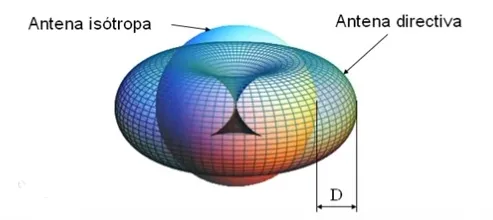
\includegraphics[width=0.7\linewidth]{Ant/Ant8.png}
\caption{Representación tridimensional de la directividad.}
\end{figure}
\begin{definition}[Ganancia de potencia]
\begin{equation}
G=\eta_A\cdot D=\frac{\mathbb{P}_{max}}{\mathbb{P}_{ref}'}
\label{eq:ganancia}
\end{equation}
Donde:
\begin{itemize}
\item \textbf{G}: Ganancia.
\item $\eta_A$: Rendimiento de la antena.
\item \textbf{D}: Directividad de la antena.
\item $\mathbb{P}_{max}$: Densidad de potencia en un punto, en la dirección de máxima radiación. ($W/m^2$)
\item $\mathbb{P}_{ref}'$: Densidad de potencia en el mismo punto, con una antena no direccional o de referencia sin pérdidas. ($W/m^2$)
\end{itemize}
\end{definition}
\begin{definition}[Factor de calidad]
\begin{equation}
Q=\frac{f_r}{BW}
\label{eq:factor de calidad}
\end{equation}
Donde:
\begin{itemize}
\item Q: Factor de calidad.
\item $f_r$: Frecuencia de resonancia. (Hz)
\item $BW$: Ancho de banda. (Hz)
\end{itemize}
\end{definition}
\subsection{Antenas receptoras}
\begin{definition}[Área de captura]
Mientras que la \textbf{ganancia de potencia} es el parametro natural para describir la mayor densidad de potencia de una señal transmitida, por las propiedades direccionales de la antena transmisora, para describir las propiedades receptiras de una antena se usa una cantidad relacionada: \textbf{área de captura}
\begin{equation}
A_{cap}=\frac{G_r\cdot\lambda^2}{4\pi}
\label{eq:area capturada}
\end{equation}
Donde:
\begin{itemize}
\item $A_{cap}$: Área efectiva de captura. ($m^2$)
\item $G_r$: Ganancia del receptor.
\item $\lambda$: Longitud de onda de la señal recibida. (m)
\end{itemize}
\end{definition}
\begin{definition}[Potencia capturada]
Potencia disponible en las terminales de salida de la antena receptora. La potencia capturada es directamente proporcional a la densidad de potencia recibida y al área de captura de la antena receptora.
\begin{equation}
P_{cap}=\mathbb{P}\cdot A_{cap}\cdot G
\label{eq:potencia capturada}
\end{equation}
Donde:
\begin{itemize}
\item $P_{cap}$: Potencia capturada. (W)
\item $\mathbb{P}$: Densidad de potencia capturada. ($W/m^2$)
\item $A_{cap}$: Área capturada. ($m^2$)
\item \textbf{G}: Ganancia.
\end{itemize}
\end{definition}
\begin{remark}
Recuerda que en todas las ecuaciones se debe trabajar con unidades \textbf{lineales}. Esto significa que todos los decibelios que nos da los problemas deben ser transformadas a sus equivalentes lineales para poder usar las ecuaciones dadas a los largo de este capitulo.
\end{remark}
\section{Transformador $\lambda$/4}
El transformador lambda-cuartos (``\textit{Quarter-Wavelength}´´) es el adaptador de impedancias más sencillo y usado para conseguir la impedancia que queremos en una línea de transmisión. Se trata de una línea de transmisión con longitud $\lambda$/4 en la frecuencia de diseño. El ancho de banda de adaptación de un transformador lambda-cuartos suele ser estrecho, aunque se puede ensanchar utilizando múltiples secciones lambda-cuartos en lugar de solo una. Por lo tanto si solo queremos que el diseño este adaptado a la frecuencia de trabajo con solo una sección nos valdría, sin embargo, si necesitamos un ancho de banda mayor en el que nuestro circuito funcione y cumpla las especificaciones, necesitaremos utilizar múltiples secciones adaptadoras.\\
\begin{notation}
Hay una demostración detrás de toda la teoría y demostración de las ecuaciones, puedes buscarlas en libros o en internet. Usaremos las ecuaciones resultantes
\end{notation}
\begin{figure}[H]
\centering
\includegraphics[width=\linewidth]{Ant/ant21.png}
\caption{Transformador $\lambda/4$.}
\label{fig:trans lambda}
\end{figure}
\textbf{Pasos para calcular}:
\begin{enumerate}
\item Normalizamos la impedancia. Ubicamos en la carta.
\item Trazamos un círculo con entro en 1 y radio el punto que trazamos anteriormente.
\item Ubicamos el cruce con el eje R más cercano. Siguiente la dirección \textit{hacia el generador}. En la parte superior de la carta tomamos como punto de referencia resistencia infinita, en la parte negativa tomamos resistencia cero. Ese valor hay que desnormalizar para hallar $Z_b$.
\item Con el valor hallado calculamos $Z_a$.
\item Con el mismo criterio del paso 3, trazamos una recta desde el centro de la carta que pase por el punto de la impedancia de carga. Hallamos la intersección de la recta y el anillo exterior "hacia el generador". Hallamos la distancia desde ese punto hacia Z=0 o Z=$\infty$ para hallar la longitud.
\end{enumerate}
\begin{example}[Se tiene una $Z_L=32-\iu 40$ con una impedancia característica de $80\Omega$. Diseñe la adaptación por $\lambda/4$.]
Normalizamos nuestra impedancia, en este caso estamos trabajando con una impedancia característica de 80 y no de 50 como casi siempre se suele hacer:
\begin{displaymath}
\overline{Z_L}=\frac{32-\iu 40}{80}=0.4-\iu 0.5
\end{displaymath}
Ubicamos la impedancia normalizada en la carta de Smith.
\begin{center}
\begin{tikzpicture}
	\begin{smithchart}[show origin]
       % Resistance plot - violet
        \addplot+[mark=*,only marks,samples at={0, -.01,...,-.5}, mark options={solid},color={violet},mark size=.2,line width=1] (0.4,x);
        % Reactance plot - blue
        \addplot[domain=0:90, samples=600, color=blue] {-.5};
        %Puntos
        \addplot+ [black,mark=o,only marks,point meta=explicit symbolic,nodes near coords] coordinates {(0.4,-0.5) [$\overline{Z_L}$]};
	\end{smithchart}
\end{tikzpicture}
\end{center}
Trazamos un circulo con centro en 1 y como radio el punto $Z_L$:
\begin{center}
\begin{tikzpicture}
	\begin{smithchart}[show origin]
        % Circle 
        \path[draw=violet] (0pt,0pt) circle (1.5cm);
        %Puntos
        \addplot+ [black,mark=o,only marks,point meta=explicit symbolic,nodes near coords] coordinates {(0.4,-0.5) [$\overline{Z_L}$] (0.32,0) [$\overline{Z_b}$]};
	\end{smithchart}
\end{tikzpicture}
\end{center}
El círculo corta la carta de Smith en dos puntos, \textbf{elegimos el más cercano}\footnote{Si estamos en la parte negativa, buscamos a R=0, si estamos en la parte positiva buscamos R=$\infty$. Sigue la dirección del anillo que indica hacia el generador.}. Ese punto es la impedancia del punto B normalizada. Desnormalizando:
\begin{displaymath}
Z_b=0.32\cdot 80=25.6\Omega
\end{displaymath}
Esto significa que la carga compleja que tenemos, en los puntos de $Z_b$ presenta una impedancia real a una distancia $\ell$. La distancia $\ell$ es hallada trazando una línea \textcolor{red}{recta} desde el origen hacia el exterior de la carta, que pase por le punto $\overline{Z_L}$:
\begin{center}
\begin{tikzpicture}
	\begin{smithchart}[show origin]
        % Circle 
        \path[draw=violet] (0pt,0pt) circle (1.5cm);
		%Line
		\addplot+ [mark size=1,red,line width=1] coordinates{(1,0) (0,-0.57)};
        %Puntos
        \addplot+ [black,mark=o,only marks,point meta=explicit symbolic,nodes near coords] coordinates {(0.4,-0.5) [$\overline{Z_L}$] (0.32,0) [$\overline{Z_b}$]};
	\end{smithchart}
\end{tikzpicture}
\end{center}
En el anillo hacia el generador, leemos el valor que resulta: 0.417 y nos movemos con la dirección que indica el anillo \textit{wavelength toward generator} hacia el eje real más cercano (en este caso R=0\footnote{Hay situaciones en la cual el más cercano es R=$\infty$, también es valido.}). Si nos recordamos, la vuelta completa es de $0.5\lambda$, para hallar esa distancia restamos:
\begin{displaymath}
\ell=0.5-0.417=0.083\lambda
\end{displaymath}
Recuerda que $\lambda$ se calcula con la ecuación \ref{eq:longitud de onda}\\
Calculando la impedancia de $\lambda/4$:
\begin{displaymath}
Z_a=\sqrt{25.6\cdot 80}=45.25\Omega
\end{displaymath}
Con ambas impedancias, solo bastaría con conseguir un cable de longitud $\lambda/4$ de impedancia $Z_a=45.25$\\
Con el transformador podemos acoplar una carga compleja o desacoplada a nuestra impedancia característica, logrando así la máxima eficiencia, máximo rendimiento, máxima transferencia de potencia, mínimo coeficiente de reflexión.
\end{example}
\chapterimage{chapter_head_ANT.pdf} % Chapter heading image
\chapter{Antenas para HF, VHF, UHF}
\section{Isotrópica}\index{Isótrópica}
La antena isotrópica es una antena hipotética sin pérdida (se refiere a que el área física es cero y por lo tanto no hay pérdidas por disipación de calor) que tiene intensidad de radiación igual en todas direcciones. (IEEE Standard Dictionary of Electrical and Electronic Terms, 1979). \\
Sirve de base de referencia para evaluar la \textbf{directividad}. La antena isotrópica no es una antena, sino un concepto de referencia para evaluar a las antenas en su función de concentración de energía y a las pérdidas por propagación en el espacio libre en los enlaces de radiofrecuencia. Su patrón de radiación es una esfera.\\
Cada aplicación y cada banda de frecuencia presentan características peculiares que dan origen a
unos tipos de antenas especiales muy diversas. Los tipos más comunes de antenas son los que se
explican en los siguientes apartados.
\section{Dipolo simétrico y asimétrico}\index{Dipolo simétrico y asimétrico}
\subsection{Diseño de un dipolo}
Vamos a diseñar un dipolo simétrico, usaremos una frecuencia de 93.5 MHz. Como vimos en teoría de la antena y usando la ecuación \ref{eq:longitud de onda} calculamos la distancia de los brazos:
\begin{wrapfigure}{r}{0.3\linewidth}
	\centering
    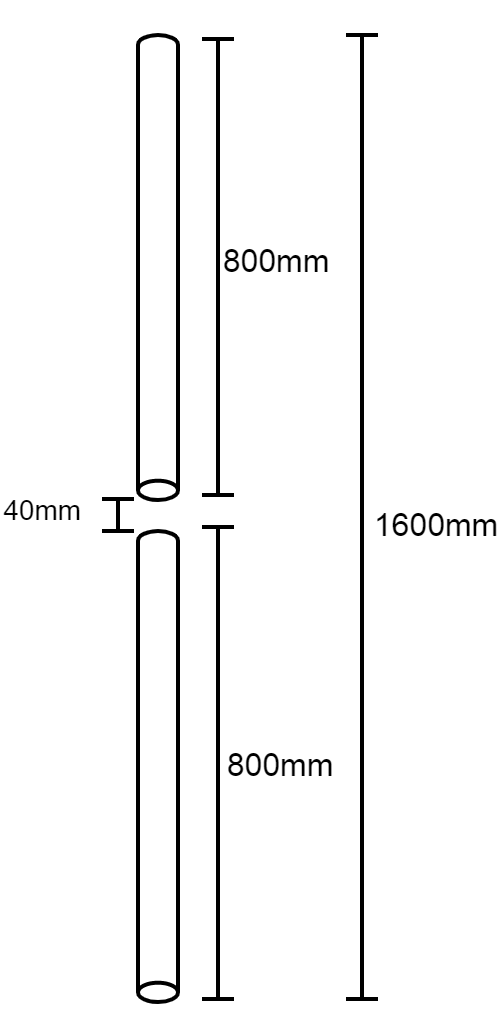
\includegraphics[width=.9\linewidth]{Ant/Ant9}
  \caption{Longitudes del dipolo.}
  \label{fig:antena dipolo medidas}
\end{wrapfigure}
\begin{displaymath}
\lambda=\frac{3\basedec{8}m/s}{93.5\basedec{6}Hz}=3.20 m\simeq 3200mm
\end{displaymath}
Con $\lambda$ calculado, podemos hallar nuestra longitud de la antena:
\begin{displaymath}
\frac{\lambda}{2}=1600mm
\end{displaymath}
Y la longitud de cada brazo es:
\begin{displaymath}
\frac{\lambda}{4}=800mm
\end{displaymath}
Ahora calcularemos el GAP\footnote{Distancia entre los brazos del dipolo simétrico}, el valor del GAP esta dado por la ecuación:
\begin{equation}
GAP=0.01\lambda
\label{eq:gap}
\end{equation}
Usando la ecuación \ref{eq:gap} calculamos nuestro valor para el GAP:
\begin{displaymath}
GAP=0.01(3200mm)=32mm\approx 40mm
\end{displaymath}
Aunque el valor nos salga 32mm, se aproxima al \textbf{múltiplo} de diez cercano o un número par. Esto ya es a criterio del ingeniero. En nuestro diseño lo hicimos a 40mm.
Resumiendo los datos en la figura \ref{fig:antena dipolo medidas}.\\
También necesitamos la caja de radiación, para esto solo agregamos la longitud de $\lambda/4$ a todos los lados:
\begin{figure}[H]
\centering
\includegraphics[width=\linewidth]{Ant/ant10_1.png}
\caption{Caja de radiación.}
\end{figure}
\begin{notation}
Nota que en la figura \ref{eq:gap}, si sumamos el GAP y longitud de ambos brazos no sale $\lambda/2$, estos valores van a ser modificador luego, son tan solo una aproximación.
\end{notation}
Con esto ya calculado, llevamos la antena al ANSYS:\\
\begin{tabular}{k{0.5\linewidth}  j{0.5\linewidth}}
        \includegraphics[width=\linewidth]{ant/ant11.png} & \textbf{Creamos un cilindro} \newline 
        En un nuevo proyecto creamos un cilindro, no importa el tamaño porque luego lo editaremos. \\
        \includegraphics[width=\linewidth]{ant/ant12.png} & \textbf{Cambiamos las propiedades} \newline 
        En el panel de objetos doble click en \textit{cylinder1} y cambiamos el nombre, material y color. Aceptar.\\
        \includegraphics[width=\linewidth]{ant/ant13.png} & \textbf{Dimensiones} \newline 
        Desplegamos el otro menu bajo \textit{BrazoL} y clickamos en CreateCylinder. Modificamos las dimensiones de acuerdo a lo calculado arriba. \textit{Center Position} es un punto relativo al cual vamos a trabajar (a modo de anclaje), aquí colocaremos la mitad del GAP, \textit{Radius} 20, pues nuestro diámetro es 40 y \textit{Height} ponemos -800, recuerda que es un dipolo, si lo situamos en el origen un brazo ira hacia los positivos y el otro hacía el positivo.\\
        \includegraphics[width=\linewidth]{ant/ant14.png} & \textbf{Duplicamos el brazoL} \newline 
        Seleccionando nuestro cilindro, vamos a \textit{Edit>Duplicate>Around Axis}, configuramos como la imagen y OK.
    \end{tabular}
   
\begin{tabular}{k{0.5\linewidth}  j{0.5\linewidth}}
        \includegraphics[width=\linewidth]{ant/ant15.png} & \textbf{Creamos la caja de radiación} \newline 
        Creamos un cilindro que cubra nuestra antena. Si la orientación del cilindro causase problemas, asegurate que el plano de referencia en la barra de herramientas este en \textbf{YZ}. Cambiamos su nombre a ``aire'', material: vacuum, color celeste y transparencia 0.9.\\
        \includegraphics[width=\linewidth]{ant/ant16.png} & \textbf{Ajustamos la caja de radiación} \newline 
        Vamos a \textit{Create Cylinder}. \textit{Center Position}: Mitad del largo de la caja de radiación (1620); \textit{Radius}: mitad del diámetro (820) y \textit{Height}: Menos la longitud de la caja de radiación (-3240).\\
         \includegraphics[width=\linewidth]{ant/ant17.png} & \textbf{Creación de puerto} \newline 
        Creamos un rectángulo en el espacio libre que dejamos entre ambas brazos. Le cambiamos el nombre a ``Puerto'' y cambiamos el color.\\
        \includegraphics[width=\linewidth]{ant/ant18.png} & \textbf{Fronteras} \newline 
        Click derecho en el cilindro creado:``aire''>Assign boundary>Radiation\\
        \includegraphics[width=\linewidth]{ant/ant19.png} & \textbf{Excitación} \newline 
        Click derecho en ``\textit{puerto}''>\textit{Assign excitation}>\textit{Port}>\textit{Lumped port}. Aceptamos la impedancia de 50 ohms. En la siguiente pantalla, en la columna \textit{integration line} por defecto estará con ``None'', lo cambiamos a \textit{new line}. Nos pedirá que tracemos una línea, trazaremos una línea por la mitad de nuestro gap desde un brazo del dipolo al otro. Ayúdate con los triángulos que aparecen cuando te encuentras a la mitad. Damos aceptar y finalizar.\\
\end{tabular}
\begin{tabular}{k{0.5\linewidth}  j{0.5\linewidth}}
        \includegraphics[width=\linewidth]{Ant/ant20.png} & \textbf{Análisis} \newline 
        En la ventana de \textit{project manager}>\textit{Analysis} (click derecho) >\textit{ Add solution setup}>\textit{Advanced}. Hemos dejado la configuración como ``Setup 1''. Colocamos nuestra frecuencia de trabajo y aceptar. En la siguiente ventana damos aceptar. Validamos el proyecto\footnote{En la pestaña \textit{Simulation}}.
\end{tabular}
\begin{tabular}{k{0.5\linewidth}  j{0.5\linewidth}}
        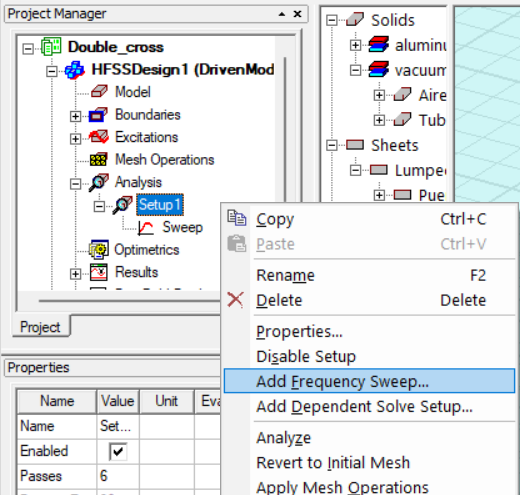
\includegraphics[width=\linewidth]{Ant/ant55.png} & \textbf{Barrido de frecuencia} \newline 
        En la ventana de \textit{project manager}>\textit{Analysis} (click derecho) > \textit{Add solution setup}. Añadimos un barrido de frecuencia, dependerá de ti los limites, trata que tu frecuencia este en el centro. Aceptar y ahora debes darle en ``Analyze all''. Esperar a que simule.
\end{tabular}
\begin{tabular}{k{0.5\linewidth}  j{0.5\linewidth}}
        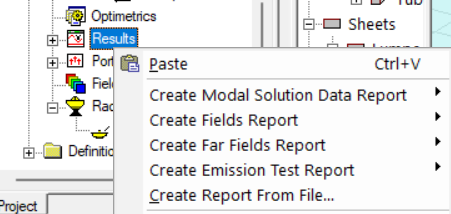
\includegraphics[width=\linewidth]{Ant/ant56.png} & \textbf{Análisis} \newline 
        En la ventana de \textit{project manager}>\textit{Result} (click derecho) > \textit{Create Modal Solution Data Report}. Usualmente se necesita ``\textit{rectangular plot}'' para los parámetros S (coeficiente de reflexión) y la carta de Smith. 
\end{tabular}
\begin{tabular}{k{0.5\linewidth}  j{0.5\linewidth}}
        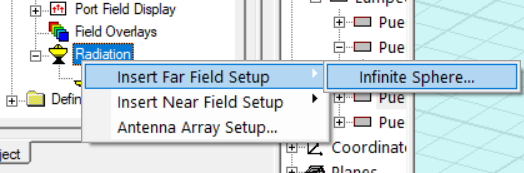
\includegraphics[width=\linewidth]{Ant/ant57.png} & \textbf{Análisis} \newline 
        Los patrones de radiación aparecerán solo si añadiste un campo lejano. Se añade en \textit{project manager}>\textit{Radiation}
\end{tabular}
\begin{definition}[Antena armónica]
Si se dispone de un número entero de semiondas, el dipolo recibe el nombre de \textbf{antena armónica}. La longitud de la antena armónica es:
\begin{equation}
l=p\cdot \frac{\lambda}{2}
\label{eq:long ant armo}
\end{equation}
Donde:
\begin{itemize}
\item \textbf{l}: Longitud de antena. (m)
\item \textbf{p}: Número de armónicos.
\item $\lambda$: Longitud de onda. (m)
\end{itemize}
\end{definition}
\subsubsection{Campo de un dipolo simétrico}
\begin{figure}[H]
\centering
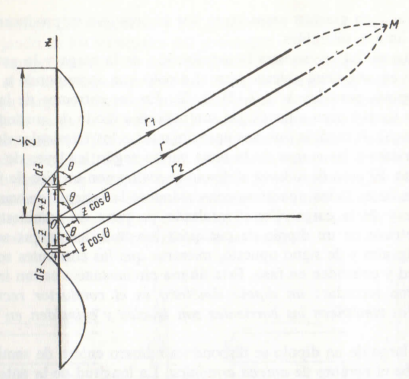
\includegraphics[width=0.7\linewidth]{ant/ant22.png}
\caption{Disposición mutua del dipolo simétrico y del punto M en el que se termina su campo de radiación.}
\end{figure}
\begin{definition}[Intensidad de campo eléctrico]
La intensidad del campo eléctrico del dipolo esta dada por:
\begin{equation}
E_{inst}=\frac{60\cdot I_m}{r}\cdot f(\theta)\cdot\sin\parentesis{\omega t-\beta r}
\label{eq:campo electrico dipolo}
\end{equation}
Donde $I_m$ es la amplitud de la corriente en el antinodo.
\end{definition}
En la ecuación \ref{eq:campo electrico dipolo}, el factor $\sin\parentesis{\omega t-\beta r}$ indica que el dipolo simétrico emite ondas progresivas. Dentro de este factor, al ángulo de fase $\omega t-\beta r$ depende de la distancia \textit{r}, pero no de $r_1$ ni de $r_2$. Esto indica que le punto medio O es el \textbf{punto equivalente de radiación} (centro de fase de todo el dipolo), y lo segundo significa que las ondas radiadas son \textbf{esféricas}.\\
La amplitud de la intensidad del campo eléctrico en la dirección del ángulo $\theta$:
\begin{equation}
E_m=\frac{60\cdot I_m}{r}f(\theta)
\end{equation}
Siendo $f(\theta)$ la función directividad del dipolo:
\begin{equation}
f(\theta)=\frac{\cos\parentesis{\frac{\pi l}{\lambda}\cos\theta}-\cos\parentesis{\frac{\pi l}{\lambda}}}{\sin\theta}
\label{eq:func theta}
\end{equation}
\begin{corollary}
La ecuación \ref{eq:func theta} es función del ángulo $\theta$, es decir, la amplitud de la intensidad de campo de un dipolo simétrico varía en el plano meridional a consecuencia de la interferencia de los campos de las secciones elementales del dipolo.
\end{corollary}


\section{Antena Marconi}\index{Marconi}
Conceptualmente, se trata de un conductor vertical de poco espesor, perpendicular a la Tierra. Puede imaginarse como un brazo de un dipolo, al cual la Tierra le sirve de espejo para "fabricar" la imagen del otro brazo del dipolo.
\begin{wrapfigure}{r}{0.45\linewidth}
  \begin{center}
    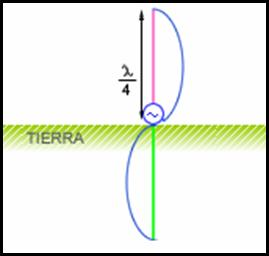
\includegraphics[width=0.8\linewidth]{ant/ant23.png}
  \end{center}
  \caption{Antena marconi}
\end{wrapfigure}
La \textbf{altura} de una antena Marconi es del orden de $\lambda/4$, con una impedancia caracteristica de $36\Omega$ y ganancia isotropica de 4.76dBi.
\begin{remark}
No confundir altura con longitud de onda de la antena. La altura es $\lambda/4$ y la longitud de onda de la antena es $\lambda/2$.
\end{remark}
Las perdidas del suelo afecta a la impedancia de la antena y el punto de eficiencia de la alimentación. Una antena de Marconi montado sobre un suelo perfectamente llevar a cabo tendría una entrada de impedancia que es la mitad de la impedancia de un dipolo, o como vimos anteriormente 36 ohms. Cuando se monta sobre un un fondo real , la impedancia de entrada puede variar de 38 ohm para una antena de radiodifusión de AM bien diseñado montado sobre un suelo preparado especialmente, a más de 100 ohm para una Marconi montada por encima, sin preparación de tierra pobre que no tiene radiales.\\
La perdida de suelo \textbf{reduce} la eficiencia de la antena, porque parte de la energía que es suministrada a la antena se disipa en el suelo en vez de ser radiada. La eficiencia puede ser calculada a partir del \textbf{valor medio de resistencia} de entrada utilizando la siguiente formula:
\begin{equation}
\eta=\frac{36}{R_{input}}
\end{equation}
\begin{remark}
El patrón de radiación de la Antena Marconi es una dona a la mitad. No existe radiación directamente hacia arriba en la dirección del cable.
\begin{center}
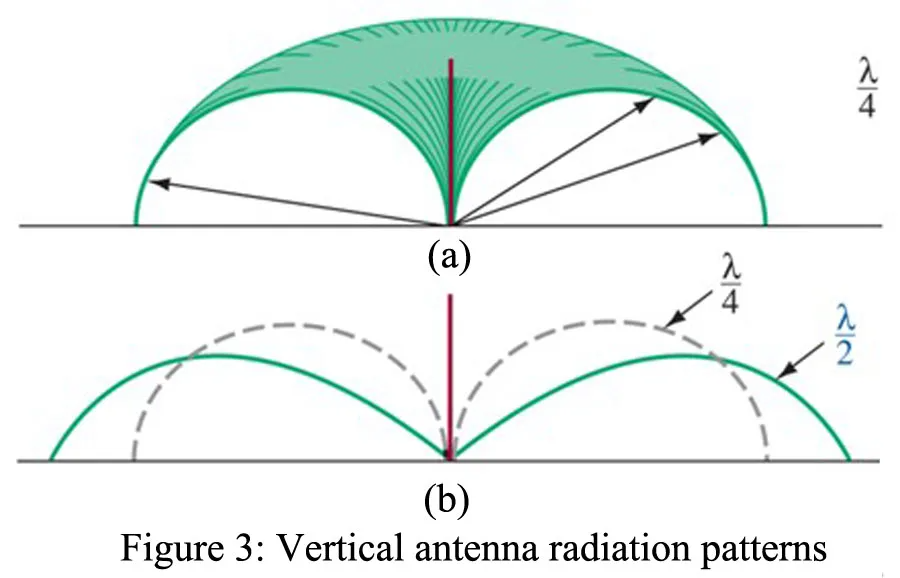
\includegraphics[width=0.7\linewidth]{ant/ant24.png}
\end{center}
\end{remark}
\subsubsection{Aplicaciones}
\begin{itemize}
\item Servicios de radio terrestre
\item Telecomunicaciones a bajas frecuencias
\end{itemize}
\section{Yagi-Uda}\index{Yagi-Uda}
\begin{figure}[H]
\centering
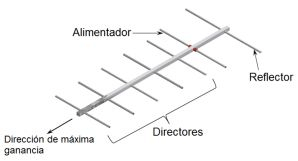
\includegraphics[width=0.6\linewidth]{ant/ant25.png}
\caption{Partes antena Yagi-Uda}
\end{figure}
\textbf{Elementos de antena}:
\begin{itemize}
\item \textbf{Excitación}: Pueden ser activos o excitados, estos se conectan directamente a la línea de transmisión y reciben potencia de la fuente.
\item \textbf{Parásitos}: No se conectan a la línea de transmisión y reciben la energía a través de la inducción mutua. Estos elementos se clasifican en reflectores y directores:
\begin{itemize}
\item \textbf{Reflector}: Elemento parásito más largo que el elemento de excitación. Reduce la intensidad de la señal que esta en su dirección e incrementa la que esta en dirección opuesta.
\item \textbf{Director}: Elementos parásitos más cortos que su elemento de excitación. Incrementa la intensidad de campo en su dirección y la reducen en la dirección opuesta.
\end{itemize}
\end{itemize}
En las antenas Yagi, la polarización depende de la posición de la antena, pudiendo ser horizontal y vertical tanto su posición como la polarización. Además en común ver un dispositivo que adapta impedancias de la línea de transmisión a la antena (más de 4 elementos).
\begin{figure}[H]
\centering
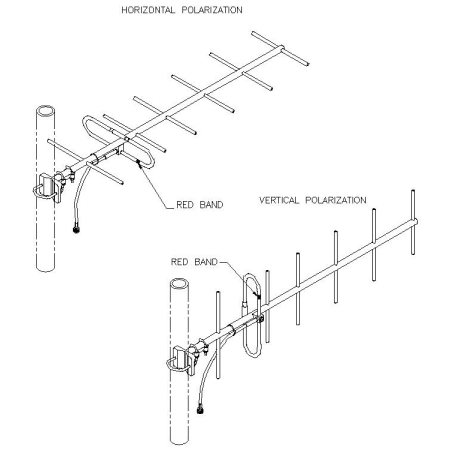
\includegraphics[width=0.7\linewidth]{ant/ant26.png}
\caption{Polarización horizontal y vertical: antena yagi.}
\end{figure}
También se puede mezclar ambas, para generar con la misma antena las dos polarizaciones a la vez. Aunque se necesitan 2 cables coaxiales (uno por antena).
\begin{figure}[H]
\centering
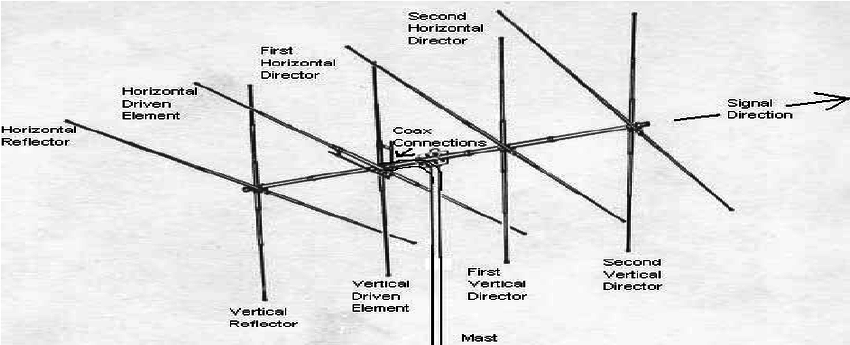
\includegraphics[width=0.7\linewidth]{Ant/ant27.png}
\caption{Doble antena Yagi.}
\end{figure}
Su \textbf{ganancia} esta dada por:
\begin{equation}
G=10\log n
\end{equation}
Donde \textit{n} es el número de elementos a considerar.\\
En cuanto a las distancias: el \textbf{reflector} es una barra de aluminio aproximadamente 5\% más larga que el dipolo, y el \textbf{director} se corta aproximadamente 5\% respecto al elemento de \textbf{excitación}. Es espacio \textbf{entre los elementos} por lo general está entre 0.1 y 0.2 longitudes de onda.\\
Directividad de una antena yagi es calculada con:
\begin{equation}
D=\frac{P_{max}}{\frac{W_t}{4\pi r2}}=\frac{4\pi r^2\cdot E_{max}^2}{I_1^2\cdot \Re{Z_{in}}\cdot\eta}
\end{equation}
\subsubsection{Aplicaciones}
\begin{itemize}
\item Las antenas Yagi Uda se emplean en la recepción de señales de TV ya que esta antena tiene una buena capacidad de recepción.
\item Utilizado en aplicaciones de defensa.
\item Empleado en el dominio astronómico.
\item También se utiliza en radioastronomía.
\end{itemize}
\section{Antenas helicoidales}\index{Helicoidal}
Antena con forma de helice a lo largo de un eje, trabaja con polarización circular y opera especialmente en el rango de 2 a 5 GHz (VHF y UHF), su diseño es muy fácil y práctico.\\
La antena helicoidal posee dos modos: \textbf{Normal} en el cual la antena de comporta similar a una antena dipolo con una radiación omnidireccional respecto al eje de la hélice; las dimensiones de la hélice son pequeñas en comparación con la longitud de onda. Luego esta la \textbf{axial}, en el cual la radiación se produce en el mismo sentido del eje de la hélice, es cuando las dimensiones de la hélice son comparables a una longitud de onda:
\begin{figure}[H]
\centering
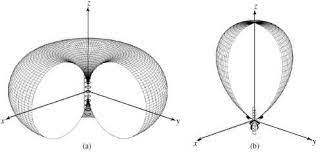
\includegraphics[width=0.7\linewidth]{ant/ant28.png}
\caption{Modos de la antena helicoidal. a. Normal b. Axial}
\label{fig:modos heli}
\end{figure}
\begin{figure}[H]
\centering
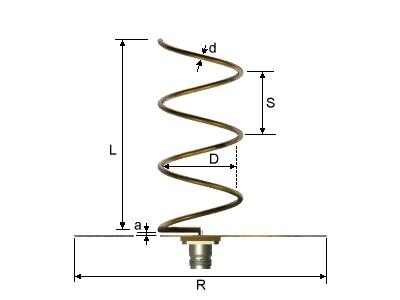
\includegraphics[width=0.7\linewidth]{ant/ant29.png}
\caption{Medidas de una antena helicoidal.}
\end{figure}
Los parametros de una antena helicoidal, generalmente son:
\begin{itemize}
\item \textbf{D}: Diámetro de giro de la hélice: Este parámetro influye en el patrón de radiación y la directividad de la antena.($\pi D$)
\item \textbf{C}: Perímetro de la circunferencia de la hélice.
\begin{equation}
C=\pi D
\end{equation}
\item \textbf{S}: Espacio entre espiras: Este parámetro determina la impedancia de la antena y el rendimiento del acoplamiento.
\item \textbf{N}: Número de vueltas de hélice: Este parámetro afecta la impedancia de la antena y su respuesta en frecuencia.
\item \textbf{L}: Paso de hélice (Pitch): Es la distancia axial entre dos puntos adyacentes en la hélice de la antena. Este parámetro determina la frecuencia de resonancia y el ancho de banda de la antena. Generalmente se toma la distancia a lo largo del eje central de la antena, en línea recta, desde el empiezo a la base. Para calcular la longitud total de toda la antena:
\begin{equation}
L_{total}=N\cdot S
\end{equation}
\item \textbf{a}: Radio del conductor: Este parámetro influye en la capacidad de manejo de potencia y la eficiencia de la antena.
\item \textbf{$L_0$}: Largo del cable. Este parámetro influye en la impedancia y pérdidas por transmisión.
\item \textbf{$\alpha$}: Ángulo de paso: Controla el crecimiento de la antena en dirección L
\begin{equation}
\alpha=\tan^{-1}\llaves{\frac{S}{C}}
\end{equation}
\end{itemize}
La antena helicoidal tiene dos modos de operación básicos:
\begin{enumerate}
\item \textbf{Modo normal}: Ocurre cuando se cumple la condición de que:
\begin{equation}
C\ll\lambda
\end{equation}
En este caso la antena puede ser modelada como una serie de pequeños dipolos y loops. Para este modo de operación la antena describe un comportamiento \textbf{omnidireccional}. La Figura \ref{fig:modos heli} (a), muestra el patrón de radiación de la antena en el modo normal
\item \textbf{Modo axial}: Ocurre cuando se cumple la condición de que:
\begin{displaymath}
C\approx\lambda
\end{displaymath}
En este modo, la antena presenta un comportamiento \textbf{direccional} y requiere de un análisis más detallado. La Figura \ref{fig:modos heli} (b) muestra el patrón de radiación en este modo de operación.
\end{enumerate}
\begin{notation}
Para el funcionamiento óptimo en modo axial:
\begin{equation}
\frac{3}{4}<\frac{C}{\lambda}<\frac{4}{3}
\end{equation}
La separación entre espiras debe ser:
\begin{equation}
S\approx\frac{\lambda}{4}
\end{equation}
\end{notation}
\begin{definition}[Ganancia de potencia]
La ganancia de potencia de una antena es una medida de su capacidad para concentrar la energía radiada en una dirección específica en comparación con una antena de referencia. Indica cuánta potencia se puede transmitir o recibir en una dirección determinada en relación con una antena isotrópica ideal y esta definida por:
\begin{equation}
A_p(dB)=10\log\corchetes{15\cdot \parentesis{\frac{D\pi}{\lambda}}^2\cdot\frac{NS}{\lambda}}
\end{equation}
Donde:
\begin{itemize}
\item $A_p(dB)$: Ganancia de la potencia de la antena. (dB)
\item \textbf{D}: Diámetro de la hélice. (m)
\item \textbf{N}: Número de vueltas.
\item \textbf{S}: Paso de la hélice. (m)
\item $\lambda$: Longitud de onda. (m)
\end{itemize}
\end{definition}
Y el ancho de haz puede ser calculado con:
\begin{definition}[Ancho de haz]
El ancho de haz en una antena helicoidal se refiere al ángulo en el cual la radiación de la antena está dentro de un rango específico de potencia o intensidad. Es la medida angular de la región en la que la antena emite o recibe señales con niveles de potencia o intensidad aceptables.
En términos prácticos, el ancho de haz determina la cobertura espacial de la antena helicoidal. Un ancho de haz más estrecho indica que la antena tiene una directividad más alta y una cobertura más enfocada en una dirección específica. Por otro lado, un ancho de haz más amplio indica una mayor cobertura en un rango angular más amplio.
\begin{equation}
\theta=\frac{52}{\frac{\pi D}{\lambda}\sqrt{\frac{NS}{\lambda}}}
\end{equation}
\begin{itemize}
\item $\theta$: Ancho de haz. (sex.)
\item \textbf{D}: Diámetro de la hélice. (m)
\item \textbf{N}: Número de vueltas.
\item \textbf{S}: Paso de hélice. (m)
\item $\lambda$: Longitud de onda. (m)
\end{itemize}
\end{definition}
\begin{definition}[Impedancia]
La impedancia dependerá del modo de la antena. Si es alimentada en su forma \textbf{axial}, la impedancia (resistiva) será\footnote{Usualmente $C$ se ve afectada, pues al momento de hallar el diametro de nuestra antena, este variará debido a que no se cuenta el material de las dimensiones requeridas por $\lambda$}
\begin{equation}
Z=140\cdot \frac{C}{\lambda}
\end{equation}
Si es alimentada de forma \textbf{normal}:
\begin{equation}
Z=\frac{140}{\sqrt{\frac{C}{\lambda}}}
\end{equation}
\end{definition}
\subsection{Aplicaciones}
\begin{itemize}
\item Radios portátiles en baja frecuencia (30-150 MHz).
\item Dispositivos inalambricos (2.425 GHz)
\item Dispositivos GSM, GPS bandas de 434 MHz, 868 MHz y 2400 MHz.
\item Radio empaquetado de alta velocidad. (S5-PSK, 1.288 Mbit/s)
\item Acceso a Internet inalámbrico de alta velocidad.
\end{itemize}
\begin{notation}
Algunas otras antenas son bocina que sirven como alimentador de parabólicas, ranuras para comunicaciones espaciales.
\end{notation}
\begin{example}[Cálculo del horizonte]
Calcule el horizonte de radio en kilómetros de una antena transmisora ubicada en lo alto de un cerro de 590 pies de altura sobre el nivel del mar en un mástil de 20 pies y la antena receptora que se halla sobre un mástil de 26 pies de altura sobre el nivel de mar.\\
\textbf{Solución:}
Tenemos dos antenas, por lo que debemos calcular el alcance de cada antena usando las ecuaciones \ref{eq:dist millas} o \ref{eq:dist km} \footnote{Dependiendo en que unidades trabajes, en este caso trabajaremos en millas y luego lo convertiremos a kilómetros.} , teniendo esas ecuaciones calculemos el alcance de cada antena:\\
\begin{align*}
d_1&=\sqrt{2(20+590)}\\
d_1&=34.93 millas\\
d_2&=\sqrt{2(26)}\\
d_2&=7.21 millas
\intertext{Sumamos ambas distancas para hallar la distancia máxima entre ellas}
d_T=34.93+7.21=42.14\simeq 67.82 Km
\end{align*}
\end{example}
\begin{example}[Cálculo de densidad de potencia]
Calcule la densidad de potencia a 32 Km de la estación transmisora, la potencia a la salida del transmisor es de 15 W, la atenuación en el conductor es 1,2 dB. La antena transmisora tiene 6.2 dB de factor de directividad y un rendimiento del 95\%.\\
\textbf{Solución:}\\
Antes de usar algún tipo de ecuación debemos analizar nuestra atenuación; nos menciona que tenemos 15 W a la salida del transmisor, luego tenemos una atenuación, es decir, se pierde energía por la línea de transmisión así que no todos los 15 W llegarán a la antena. Tenemos dos formas de formas de calcular la potencia que llegará a la antena. Primero la calculamos usando solo unidades lineales:
\begin{displaymath}
P[W]=\frac{P_{T_x}[W]}{At}
\end{displaymath}
Como estamos trabajando con unidades lineales, debemos convertir la atenuación que originalmente esta en decibelios a unidades lineales, para ello:
\begin{displaymath}
At=10^{\frac{1,2 dB}{10}}=1,32
\end{displaymath}
Ahora recién con este valor podemos hallar la potencia que llega a la antena tomando en cuenta la atenuación:
\begin{displaymath}
P[W]=\frac{15 W}{1,32}=11,36 W
\end{displaymath}
La \textbf{segunda manera} de hallar la potencia de la antena es hallando  el valor en unidades de decibelios; planteando la potencia en dB debemos de considerar que ahora las unidades no se deben dividir, se \textbf{deben restar}, esto se puede demostrar usando las propiedades de los logaritmos (esto no de desarrollará pues ya es bien sabido como). Sin perder la formalidad de las matemáticas, lo podemos expresar como:
\begin{displaymath}
P_A[dBW]=P_{T_x}[dBW]-  At[dB]
\end{displaymath}
Ahora debemos que usar nuestra potencia en unidades de decibelios, para ello:
\begin{displaymath}
P_{T_x}[dBW]=10\cdot\log 15=11,76 dBW
\end{displaymath}
Ahora que todos los datos están en las mismas unidades, efectuamos la operación:
\begin{displaymath}
P_A[dBW]=11,76 dBW - 1,2 dB=10,56 dBW\simeq 11,38 W
\end{displaymath}
Hay una pequeña diferencia entre ambas más mientras no afecte significativamente a los cálculos es aceptable.\\
Calcularemos la intensidad de campo usando la ecuación \ref{eq:int campo}, notaremos de acuerdo a la ecuación \ref{eq:pire}, PIRE puede ser calculado de dos maneras, nosotros tenemos potencia de antena, por lo que nos falta ganancia que puede ser calculada facilmente con la ecuación  \ref{eq:ganancia}:
\begin{displaymath}
G=0,95\cdot 10^{\frac{6,2}{10}}=3,96
\end{displaymath}
Teniendo en cuenta que debe ser en unidades lineales, por eso convertimos la directividad de decibelios a lineales.\\
Con la ganancia hallada y usando la ecuación \ref{eq:int campo}:
\begin{displaymath}
\mathbb{P}=\frac{11,36 W\cdot 3,96}{4\cdot\pi\cdot(32\basedec{3})^2}=3,5 mW/m^2
\end{displaymath}
\end{example}
\begin{example}[Intensidad de campo eléctrico]
Si la intensidad del campo eléctrico en la zona de recepción a 21 Km de la estación transmisora es de 1,1 mV/m, cuanto debe ser la ganancia de la antena transmisora expresada en dB, si la potencia a la entrada de la antena transmisora es de 1,5 W.\\
\textbf{Solución:}\\
Teniendo en cuenta las ecuaciones \ref{eq:pire} y \ref{eq:int campo} podemos despejar la siguiente expresión:
\begin{displaymath}
\frac{P_A\cdot G}{4\pi\cdot r^2}=\frac{E^2}{Z_S}
\end{displaymath}
Reemplazando los valores que tenemos en la expresión:
\begin{displaymath}
\frac{1.5 W\cdot G}{4\pi\cdot (12\basedec{3})^2}=\frac{(1.1\basedec{-3})^2}{377 \Omega}
\end{displaymath}
Despejando la ganancia de esta ecuación:
\begin{displaymath}
G=\frac{(1.1\basedec{10^{-3}})\cdot 4\pi\cdot (12\basedec{3})^2}{377\cdot 1,5}=3.87
\end{displaymath}
Sin embargo nos pides la respuesta en decibelios:
\begin{displaymath}
G[dB]=10\log(3.37)=5.88 dB
\end{displaymath}
\end{example}
\begin{corollary}[Características del diagrama de radiación de un dipolo horizontal próximo a un plano de tierra.]
Son:
\begin{itemize}
\item Un dipolo horizontal colocado sobre una pantalla irradia, igual que un dipolo aislado, ondas esféricas progresivas con centro de fases en el punto medio entre el dipolo y su imagen eléctrica.
\item Un dipolo horizontal colocado a cualquier altura \textit{h}, no irradia a lo largo de la superficie de la pantalla.
\item En los diagramas de directividad del dipolo horizontal sobre la pantalla conductora, se tiene igualdad de máximos y la presencia de mínimos nulos en los lóbulos del diagrama.
\end{itemize}
\end{corollary}
\begin{corollary}[Características constructivas de las antenas periodo logarítmicas]
Es una antena conformada por barios dipolos que resuenan a distintas frecuencias, que la hace como una antena de banda ancha. El esparcimiento entre dipolos es variable y la alimentación se hace desde el elemento más corto. 
\end{corollary}
\chapterimage{chapter_head_ANT.pdf} % Chapter heading image
\chapter{Radioenlace de microondas}
\section{Guías de onda}\index{Guías de onda}
\begin{wrapfigure}{r}{0.4\linewidth}
  \begin{center}
    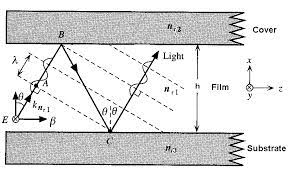
\includegraphics[width=.9\linewidth]{Ant/ant30.png}
  \end{center}
  \caption{Propagación de OEM por la guía de onda.}
\end{wrapfigure}
En electromagnetismo y en telecomunicaciones, una guía de onda es cualquier estructura física que guía ondas electromagnéticas. Una guía de ondas o guíaondas, es un tubo conductor hueco, por lo general de corte transversal rectangular, a veces circular o elíptico. Son adecuadas para transmitir señales debido a sus \textbf{bajas pérdidas}, sin embargo cuentan con ancho de banda limitado y volumen mayor que líneas coaxiales.\\
Es importante que sepas que las guías de onda no conducen corriente en el sentido estricto, sino mas bien sirve como una frontera para confinar la energía electromagnética; las OEM se reflejan (su energía) en la superficie interior.
Para lograr una baja resistencia y por ende con pérdidas de transmisión a un nivel bajo, estas guías de onda deben ser fabricadas de cobre, aluminio o bronce.\\
\subsection{Conceptos generales}
Las ecuaciones de Maxwell tienen soluciones múltiples, o modos: $E=0$ y $H_n=0$. Los \textbf{modos de propagación} dependen de la longitud de onda, de la polarización y de las dimensiones de la guía. El \textbf{modo longitudinal} de una guía de onda es un tipo particular de onda estacionaria formado por ondas confinadas en la cavidad. \\
En la \textbf{línea de transmisión}, la velocidad de la onda \textbf{depende del dieléctrico}, mas no de la velocidad de la onda; en la \textbf{guía de onda}, la velocidad varía en \textbf{función de la frecuencia}.
\begin{definition}[Velocidad de fase]
\begin{equation}
V_{ph}=f\cdot\lambda
\label{eq:velfase}
\end{equation}
Donde:
\begin{itemize}
\item $V_{ph}$: Velocidad de fase. (m/s)
\item f: Frecuencia. (Hz)
\item $\lambda$: Longitud de onda. (m)
\end{itemize}
\end{definition}
\begin{definition}[Velocidad de grupo]
\begin{equation}
V_g=\frac{c^2}{V_{ph}}
\label{eq:velgrup}
\end{equation}
\begin{itemize}
\item $V_g$: Velocidad de grupo. (m/s)
\item c: Velocidad de la luz $3\times\basedec{8}$ (m/s)
\end{itemize}
La longitud de onda en la guía puede ser calculada con:
\begin{equation}
\lambda_g=\lambda_0\parentesis{\frac{V_{ph}}{c}}=\frac{c}{\sqrt{f^2-f_c^2}}=\frac{\lambda_0}{\sqrt{1-\parentesis{\frac{f_c}{f}}^2}}
\end{equation}
Donde:
\begin{itemize}
\item $\lambda_g$: Longitud de onda en la guía. (m)
\item $\lambda_0$: Longitud de onda en el espacio libre. (m)
\item $V_{ph}$: Velocidad de fase. (m/s)
\item c: Velocidad de la luz. (m/s)
\item f: Frecuencia de operación. (Hz)
\item $f_c$: Frecuencia de corte. (Hz)
\end{itemize}
\end{definition}
Combinando las ecuaciones anteriores se puede obtener la velocidad de fase como:
\begin{equation}
V_{ph}=\frac{c\cdot\lambda_g}{\lambda_0}=\frac{c}{\sqrt{1-\parentesis{\frac{f_c}{f}}^2}}
\end{equation}
\subsection{Inyección y extracción de señales}
Para realizar la \textbf{inyección} se una señal de microondas en una guía, en el extremo de la guía se introduce una sonda tipo de antena que produce una OEM, los campos eléctricos y magnéticos se combinan con la señal, rebotan en el interior de las paredes viajando por la guía de onda. En este medio \textbf{no hay perdidas por radiación}. La sonda que alimenta la guía de onda, es una antena vertical de \textbf{un cuarto de longitud de onda}. La posición de la sonda determina si la señal está polarizada de manera horizontal o vertical. Para la inyección de onda también se suelen usar \textbf{aros}; para la \textbf{extracción} se usan ambos modos: sondas o aros.
\subsection{Guía de onda rectangular}
\begin{figure}[H]
\centering
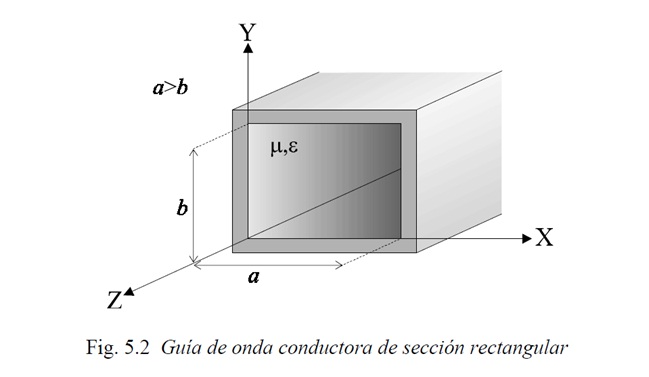
\includegraphics[width=0.7\linewidth]{Ant/ant31.png}
\caption{Guía de onda rectangular}
\end{figure}
La frecuencia de operación de una guía de onda la determina el ancho de esta (a), la dimensión de la guía se hace a lambda medios, un poco más bajo de la frecuencia de operación más baja o frecuencia de corte. Por debajo de esta \textbf{frecuencia de corte} la guía de onda no transmitirá energía.\\
La guía de onda es considerada como un \textbf{filtro pasa alto} debido a esta característica de funcionar solo a frecuencias por encima de la frecuencia de corte. La \textbf{frecuencia de corte} puede ser calculada con:
\begin{equation}
f_{c}=\frac{c}{2a}
\end{equation}
Teniendo en consideración que el ancho de la guía (a) debe estar en metros.\\
Generalmente el alto de la guía (b) es la mitad del ancho: b=a/2.\\
El corte se presenta a la frecuencia para la cual la dimensión transversal máxima de la guía, es la mitad de la longitud de la onda en el espacio libre ($\lambda_{co}$):
\begin{equation}
\lambda_{co}=2a
\end{equation}
\subsubsection{La propagación de la señal}
Cuando la sonda envía energía por la guía de onda, la señal se propaga usando el principio de reflexión de la ley de Snell. Una sonda vertical genera una \textbf{onda polarizada en forma vertical} con un campo eléctrico \textbf{vertical} y un campo magnético en \textbf{ángulo recto} con el campo eléctrico formando un ángulo recto, incluso con la dirección de propagación de la onda; por lo que se llama \textbf{campo eléctrico transverso (TE)}.\\
En caso de que el campo magnético es \textbf{perpendicular} a la dirección de propagación, se denomina \textbf{campo magnético transverso (TM)}.
\begin{figure}[H]
\centering
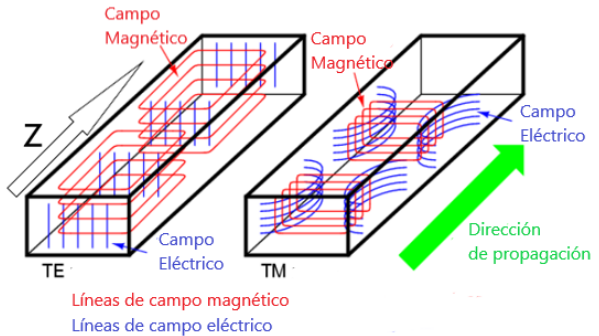
\includegraphics[width=0.8\linewidth]{Ant/ant32.png}
\caption{Modos de transmisión}
\end{figure}
En el modo TE, el campo eléctrico existe a través de la guía y no hay línea E que se extiendan en forma longitudinal a lo largo de la guía, los vectores E son \textbf{perpendiculares} a las paredes de la guía.
En el modelo TM, las líneas H forman aros en planos \textbf{perpendiculares} a las paredes de la guía y ninguna parte de una línea H se extiende de manera longitudinal a lo largo de la guía.
\begin{notation}
Los ángulos de incidencia y reflexión dependen de la frecuencia de operación. Conforme la frecuencia de operación decrece, el ángulo también lo hace, y la trayectoria entre los lados se vuelve más corta.
Cuando la frecuencia de operación alcanza la frecuencia de corte de la guía de onda, la señal solo bota de un lado a otro entre las paredes laterales de la guía de onda. No se propaga energía.
\end{notation}
La forma en que los campos eléctrico y magnético se propagan en el interior de la guía de onda depende de: 
\begin{itemize}
\item El método de acoplamiento de la energía  (sonda o aro).
\item De la frecuencia de operación.
\item Del tamaño de la guía de onda.
\end{itemize}
Con la designación de TE y TM se usan subíndices para describir mejor los patrones del campo E y H. Una designación típica es $TE_{m,n}$; el primer número entero (\textit{m}) indica la \textbf{cantidad de patrones} de $\lambda/2$ de líneas perpendiculares a la pared de la guía, que existen a lo largo de la dimensión mayor de la guía (sección \textit{a}) a través de la sección transversal. El segundo número (\textit{n}) indica la cantidad de patrones transversales de $\lambda/2$ que existen a lo largo de la dimensión menor de la guía (sección \textit{b}) a través de la sección transversal. Si no hay cambio en la intensidad del campo de una dimensión se usa Cero.\\
El modo $TE_{1,0}$ se llama ``modo dominante'' por ser el más natural. La guía de onda rectangular se suele trabajar dentro de los márgenes de frecuencia de $f_c$ a $2f_c$. En caso de trabajar en modos superiores de propagación, esta no se acopla bien con la carga, y se provocan reflexiones y creación de ondas estacionarias.
\subsection{Guía de onda circular}
Las guías de onda circulares son mas fácil de fabricar que las rectangulares, y mas fácil de empalmar. Las guías circulares tienen un área mucho mayor que una rectangular correspondiente, para llevar la misma señal. Otra desventaja de la guía circular es la variación de la polarización mientras la onda se propaga por ella.\\
Se usan en radar y en aplicaciones de microondas, cuando hay ventaja de propagar ondas polarizadas vertical y horizontalmente en la misma guía.
El comportamiento de las ondas electromagnéticas en las guías de onda circulares es igual que las rectangulares. El modo de propagación $TE_{1,1}$ es el dominante en las guías de onda circulares, para este modo la longitud de onda de corte es:
\begin{equation}
\lambda_0=1.7d
\label{eq:onda de corte circular}
\end{equation}
Donde \textit{d} esta en metros y es el diámetro de la guía de onda. La longitud de corte de la ecuación \ref{eq:onda de corte circular} es medida en metros.
\section{Antenas de bocina}\index{Bocina}
Las antenas de bocina son unas antenas que realizan la transición desde el medio guiado (guías de onda) al espacio libre. Las bocinas se utilizan en los satélites principalmente como alimentadores de los reflectores y en algunas ocasiones se utilizan como antenas simples cuando se requieren grandes anchos de haz. Las antenas de bocina se utilizan frecuentemente para conformar haces que den una cobertura terrestre. 
El ancho de haz necesario par dar cobertura a la tierra desde la órbita geoestacionaria es de 18 grados, que es fácilmente realizable con antenas de bocina.\\
Si una dimensión del tubo es mayor que media longitud de onda, entonces la onda puede propagar a través de la guía de onda con la perdida sumamente baja, y si al ser colocada el final de una guía de onda simplemente es dejado abierto, la onda irradiara al espacio.
\begin{figure}[H]
\centering
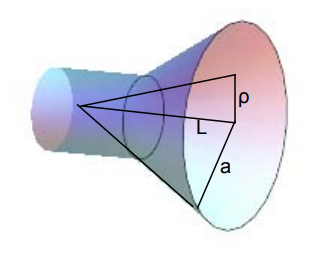
\includegraphics[width=.5\linewidth]{Ant/ant33.png}
\caption{Antena bocina circular.}
\end{figure}
\begin{equation}
D=\frac{4\pi}{\lambda^2}A_{ef}=\frac{4\pi}{\lambda^2}\parentesis{\pi a^2}\eta_{il}
\end{equation}
\begin{figure}[H]
\centering
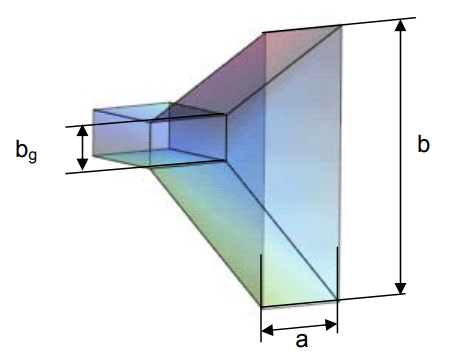
\includegraphics[width=0.6\linewidth]{Ant/ant34.png}
\caption{Antena bocina rectangular.}
\end{figure}
\begin{equation}
D=\frac{4\pi}{\lambda^2}A_{ef}=\frac{4\pi}{\lambda^2}ab\eta_{il}
\end{equation}
\subsection{Tipos de bocina}
Existen dos tipos más usadas: rectangulares y cónica:
\subsubsection{Bocinas rectangulares}
Adecuada para sistemas de polarización lineal, ya que minimiza las perdidas y reduce la generación de modos de ordenes superiores que afecten al comportamiento de la eficiencia y de la polarización. Tiene la ventaja de transmitir ondas sin polarización cruzada, que junto con el hecho de que su ganancia se puede calcular exactamente a partir de sus dimensiones.
\subsubsection{Bocina cónica}
Son las que se utilizan fundamentalmente en antenas de satélites de haz global. Son las más adecuadas para utilizar polarizaciones circulares, aunque también pueda utilizar polarizaciones lineales, estas polarizaciones tienen un mejor comportamiento en las bocinas piramidales. Se pueden clasificar según el modo de propagación transmitido: bocinas de modo dominante, bocinas de modo dual y bocinas corrugadas. 
Las \textbf{bocinas de modo dual} se han desarrollado para obtener un ancho de haz igual en los planos E y H, con un bajo nivel de polarización cruzada. En este tipo de bocinas, los modos $TE_{11}$ y $TM_{11}$ son combinados con apropiadas relaciones de amplitud y diferencias de fase en su apertura.\\
Otra variante de las bocinas son las bocinas de \textbf{modos híbridos}. Corrugando la pared interior de una bocina cónica se consigue que no se propaguen ni los modos TE ni los TM, sino que se crean en la bocina unos modos híbridos. Estas antenas mejoran la polarización cruzada y el nivel de los lóbulos secundarios, otra característica remarcable es que consiguen anchos de haz simétricos respecto al eje de la bocina.\\
Bocinas de \textbf{modo dominante} (o de modo único): Se sintoniza al modo predominante de la guía de onda circular. Este es el más básico de los tres tipos.
Bocinas de modo dual (o multimodo): Se sintoniza al modo  de propagación de la onda que se propaga por la guía de onda.\\
Estas bocinas se utilizan extensamente en satélites comerciales. Pero la utilización más común de las bocinas es como un \textbf{elemento de radiación} para reflectores de antenas. La bocina se sitúa en el \textbf{foco} o en un lugar próximo a él de un reflector \textbf{parabólico} para iluminar su superficie tanto en la aplicación de transmisión como en recepción. La radiación electromagnética en la superficie del reflector produce corrientes eléctricas en la superficie. Y de estas corrientes se producen otros campos electromagnéticos que finalmente se convierten en un diagrama de radiación de campo lejano del sistema de antena total.
\section{Antenas de ranura}\index{Ranura}
Se llaman antenas de ranura aquellas en que la radiación y la recepción de las ondas electromagnéticas se realizan mediante unas o varias ranuras practicadas en una guía de ondas o un resonador volumétrico.
%Antenas de ranura
\section{Antenas reflector parabólico}
Cuando se desea la máxima \textbf{directividad} de una antena, la forma del reflector generalmente es parabólica, con la fuente primaria localizada en el foco y dirigida hacia el reflector. Las antenas con reflector parabólico, o simplemente antenas parabólicas se utilizan extensamente en sistemas de comunicaciones en las bandas de \textbf{UHF} a partir de unos 800 MHz y en las de SHF y EHF. Entre sus características principales se encuentran la sencillez de construcción y \textbf{elevada direccionalidad}. La forma más habitual del reflector es la de un paraboloide de revolución, excitado por un alimentador situado en el foco como se ilustra en la figura \ref{fig:ant par}.
\begin{figure}[H]
\centering
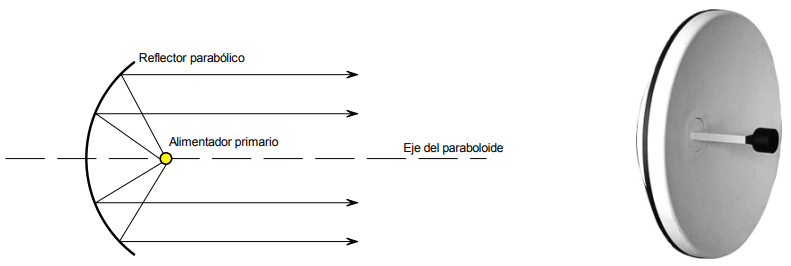
\includegraphics[width=0.6\linewidth]{ant/ant47.png}
\caption{Antena con reflector parabólico}
\label{fig:ant par}
\end{figure}
Otro tipo de antena, bastante utilizado en aplicaciones de radar es el cilindro parabólico que tiene la forma mostrada en la figura \ref{fig:ref cilin} y fue la primera antena con reflector utilizada por Hertz en sus experimentos. El alimentador, o fuente de energía es una antena lineal o un alineamiento de éstas, colocada en la línea focal y la reflexión en la superficie parabólica transforma el frente de onda de cilíndrico en plano.
\begin{figure}[H]
\centering
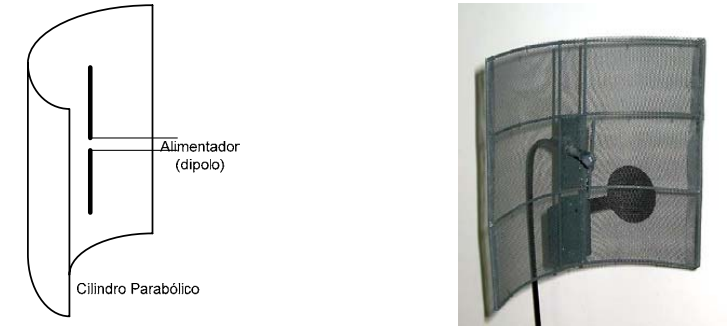
\includegraphics[width=0.6\linewidth]{ant/ant48.png}
\caption{Cilindro parabólico}
\label{fig:ref cilin}
\end{figure}
En las antenas parabólicas se aplican las propiedades ópticas de las ondas electromagnéticas. Las propiedades geométricas de la parábola son tales que las ondas emitidas por el alimentador en el foco se reflejan por la parábola en un haz de rayos paralelos al eje de la parábola, de modo que la longitud del trayecto del foco al reflector parabólico y, después, hasta la superficie de la abertura que pasa por los bordes de la parábola, es la misma para cualquier ángulo. Por consecuencia en la abertura de la antena se tiene una superficie equifase y, teóricamente, el haz radiado es cilíndrico, si bien en la práctica esto no es completamente cierto, ya que parte de la energía se dispersa en los bordes del reflector. En la figura \ref{fig:geo para} se ilustra la geometría de la antena parabólica.
\begin{figure}[H]
\centering
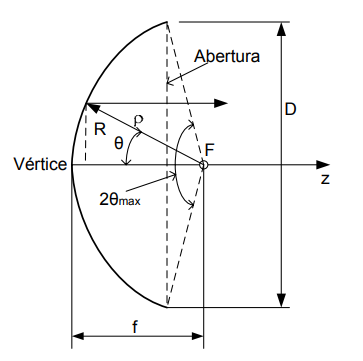
\includegraphics[width=0.6\linewidth]{ant/ant49.png}
\caption{Geometría de la parábola}
\label{fig:geo para}
\end{figure}
Un defecto de las antenas parabólicas con el alimentador en el foco lo constituye el hecho de que el alimentador obstruye los rayos reflejados produciendo un región de baja intensidad o sombra en el centro de la apertura. El efecto en el patrón de radiación puede estimarse aproximadamente tomando la diferencia de la radiación de la abertura y del área de sombra localizada en la dirección del alimentador. El efecto neto es una alteración del patrón de radiación en que se rellenan los nulos entre lóbulos como se ilustra en la figura \ref{fig:sombra rad} en coordenadas rectangulares.
\begin{figure}[H]
\centering
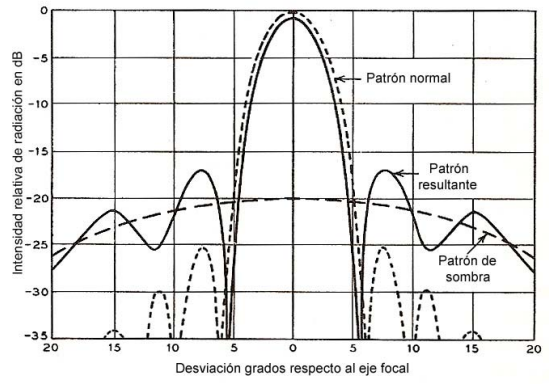
\includegraphics[width=0.6\linewidth]{ant/ant50.png}
\caption{Efecto de la sombra en el patrón de radiación}
\label{fig:sombra rad}
\end{figure}
Otro efecto que se produce cuando el alimentador está en la trayectoria de la onda reflejada es que algo de la energía de ésta regresa al sistema alimentador y produce un desacoplamiento de impedancia. El valor absoluto de la impedancia es prácticamente constante en función de la frecuencia o de la posición del alimentador, pero su fase puede variar rápidamente debido al viaje de ida y vuelta del alimentador al reflector y de regreso a éste. Un método para evitar este problema de impedancia, así como la sombra producida por el alimentador es  desplazar éste como se ilustra en la figura \ref{fig:offset}. En este tipo de antena para todos los fines prácticos, el alimentador queda fuera de la onda reflejada.
\begin{figure}[H]
\centering
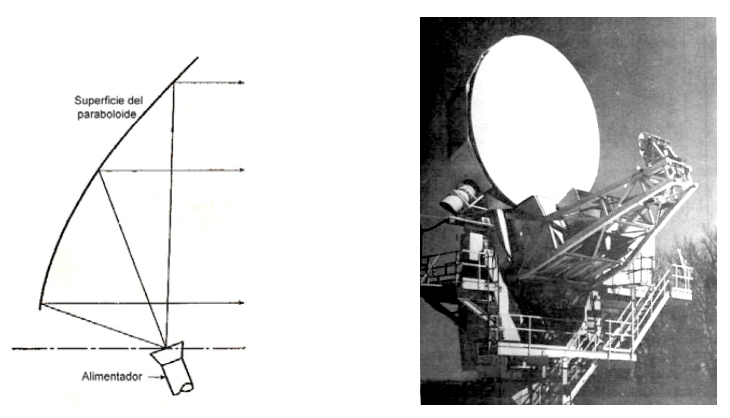
\includegraphics[width=0.6\linewidth]{ant/ant51.png}
\caption{Antena parabólica con foco desplazado: \textit{offset}.}
\label{fig:offset}
\end{figure}
\begin{definition}[Ganancia de una antena parabólica]
La ganancia teórica de una antena parabólica de abertura circular excitada uniformemente está dada por:
\begin{equation}
G=\eta\parentesis{\frac{\pi\cdot D}{\lambda}}^2
\label{eq:ganancia para}
\end{equation}
Donde:
\begin{itemize}
\item \textbf{G}:Ganancia
\item \textbf{D}: Diámetro de la antena. (m)
\item $\lambda$: Longitud de onda. (m)
\item $\eta$: Eficiencia
\end{itemize}
\end{definition}
En la eficiencia de cualquier antena y, en particular de las antenas parabólicas intervienen diversos factores como los mencionados en párrafos anteriores y otros como las pérdidas óhmicas, la dispersión en los bordes, la obstrucción y dispersión por los diversos elementos estructurales que soportan el alimentador o el subrreflector en el caso de antenas Cassegrain que se tratarán más adelante, rugosidad de la superficie reflectora, etc.
\begin{definition}[Directividad]
\begin{equation}
D=4\pi\parentesis{\frac{L}{\lambda}}^2
\label{eq: direc para}
\end{equation}
Donde:
\begin{itemize}
\item \textbf{D}: Directividad.
\item \textbf{L}: Abertura de lado L. (m)
\item $\lambda$: Longitud de onda. (m)
\end{itemize}
\end{definition}
\begin{notation}
No confundir la letra D de las ecuaciones \ref{eq:ganancia para} t \ref{eq: direc para}, en la primera representa distancia y en la segunda representa directividad.
\end{notation}
\subsection{Antenas \textit{offset}}
Antenas en las que la estructura de soporte del alimentador no presenta obstrucción significativa al haz reflejado por el paraboloide como se ilustra en la figura \ref{fig:geo antena offset}. Aunque hay cierta ambigüedad en el uso del término offset en la ingeniería de antenas, aquí entenderemos que una antena offset es aquella que no es simétrica respecto al eje de revolución, ya que se descarta la porción de la superficie reflectora situada a un lado del eje. Como el alimentador debe estar localizado sobre el eje o muy cerca de él, en la antena offset se desplaza al alimentador de la región de máxima abertura, reduciendo o eliminando el bloqueo. Desde luego, el eje del alimentador debe desplazarse verticalmente de modo que el haz transmitido por él incida sobre la superficie de la porción reflectora del paraboloide, ya que otro modo se produce un desborde excesivo en los bordes del reflector.
\begin{figure}[H]
\centering
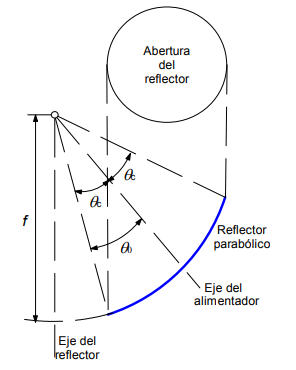
\includegraphics[width=0.6\linewidth]{ant/ant52.png}
\caption{Geometría de una antena offset.}
\label{fig:geo antena offset}
\end{figure}
\begin{definition}[BDF]
La relación entre el ángulo del haz y el del alimentador se designa como factor de desviación del haz (BDF) y se puede calcular como:
\begin{equation}
BDF=\frac{\sin^{-1}\corchetes{\frac{d}{f}\cdot\frac{1+k\parentesis{\frac{D}{4f}}^2}{1+\parentesis{\frac{D}{4f}}^2}}}{\tan^{-1}\parentesis{\frac{d}{f}}}
\end{equation}
Donde:
\begin{itemize}
\item \textbf{d}: Distancia entre la posición del alimentador en el eje horizontal perpendicular al del paraboloide. (m)
\item \textbf{D}: Diámetro del paraboloide. (m)
\item \textbf{f}: Distancia focal. (m)
\item \textbf{k}: Constante menor que 1.
\end{itemize}
\end{definition}
\subsection{Antenas con doble reflector: Cassegrain}
\subsubsection{Antenas doble reflector}
Las antenas con doble reflector están constituidas por dos reflectores, uno principal parabólico y otro secundario, en la forma que se ilustra esquemáticamente en la figura \ref{fig:doble reflec}.
\begin{figure}[H]
\centering
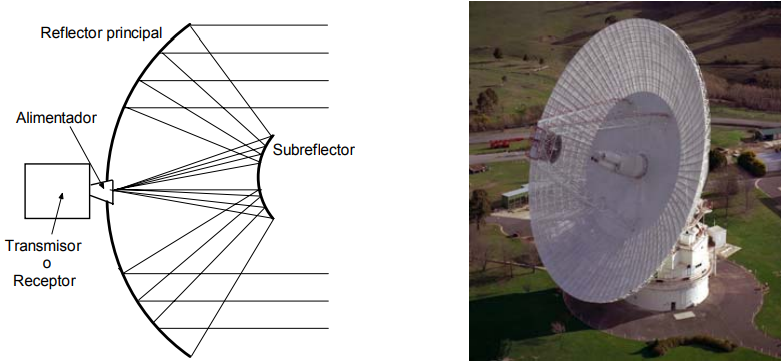
\includegraphics[width=0.6\linewidth]{ant/ant53.png}
\caption{Geometría básica de una antena de doble reflector.}
\label{fig:doble reflec}
\end{figure}
El subreflector suele ser hiperbólico en cuyo caso la antena se designa como Cassegrain16 o bien elíptico y la antena se designa como gregoriana17. En la primera, el hiperboloide suele presentar la parte convexa hacia el reflector principal como en el caso de la figura \ref{fig:ant par} y, en la gregoriana, el elipsoide reflector suele presentar la parte cóncava. En algunos casos se emplean también subreflectores planos o esféricos. Estas antenas se utilizan extensamente en comunicaciones espaciales y radioastronomía, además de comunicaciones terrestres. Este
tipo de antenas ofrece algunas ventajas sobre las antenas de un solo reflector y, aunque pueden tener diseños diferentes, comparten un conjunto de aspectos básicos comunes. Una de
las ventajas es que el alimentador de la antena no requiere de una línea de transmisión larga y se conecta casi directamente a la salida del transmisor o a la entrada del receptor reduciendo considerablemente las pérdidas. Si bien el bloqueo por la estructura de soporte no puede eliminarse en el caso de la geometría de la figura \ref{fig:ant par}, la eficiencia de las antenas de doble reflector en general es superior a la de las de reflector simple llegando aproximadamente al
70\% o más. Su ganancia se calcula de la misma manera que la una antena parabólica simple, utilizando la ecuación \ref{eq:ganancia para}.
\subsubsection{Antena Cassegrain}
Un telescopio Cassegrain consiste de dos espejos y un instrumento óptico de observación. El espejo primario es grande y cóncavo y refleja la luz incidente hacia un espejo secundario convexo y más pequeño, frente al espejo primario. Este espejo secundario refleja a su vez la luz hacia el centro del espejo primario en el que sitúa el observador o, en al caso de una antena, el receptor, como se ilustra esquemáticamente en la figura \ref{fig:doble reflec}.\\
El subreflector debe ser lo suficientemente grande como para interceptar la porción útil de la radiación del alimentador y refleja esta onda sobre el reflector primario de acuerdo a las leyes de la óptica. En la geometría clásica de la antena Cassegrain se emplea un paraboloide como reflector primario o principal y un hiperboloide para el reflector secundario en que uno de los dos focos de la hipérbola es el punto focal real del sistema y está localizado en el centro del alimentador. El otro es un foco virtual que se localiza en el foco de la parábola. Como resultado, todas las partes de la onda originada en el foco real y luego que luego son reflejadas por ambas superficies, viajan distancias iguales hasta el plano de la abertura frente a la antena.
\begin{figure}[H]
\centering
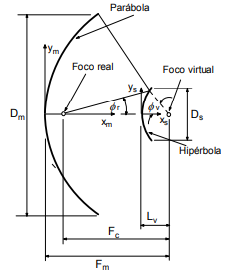
\includegraphics[width=0.4\linewidth]{ant/ant54.png}
\caption{Geometría antena Cassegrain.}
\end{figure}
\section{Antenas Parche}\index{Parche}
Microstrip o antenas de parches son cada vez más útiles porque se pueden imprimir directamente sobre una placa de circuito. Ellos son cada vez más generalizada en el mercado de la telefonía móvil. Son de bajo coste, tienen un perfil bajo y se fabrican fácilmente. La tendencia a la miniaturización al lograr dispositivos cada vez mas pequeños, de fácil producción en masa (costos reducidos), fáciles de adaptar con circuitos integrados de microondas, versátiles en términos de impedancia, patrón, polarización y frecuencia de resonancia. Dentro de las desventajas podemos encontrar la baja potencia de radiación (por su estructura no se puede soportar grandes potencias en su estructura), baja eficiencia, ancho de banda angosto para ciertos diseños, considerables perdidas y son fácilmente afectadas por el factor térmico (sobre todo si se trabaja en sustratos flexibles).
\subsection{Características}
\begin{figure}[H]
\centering
\subfloat[Vista superior]{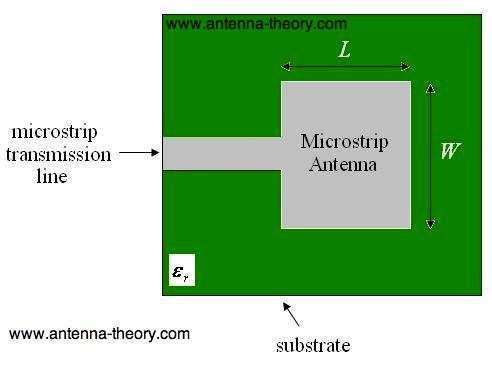
\includegraphics[width=0.4\linewidth]{ant/ant35.png}}
\subfloat[Vista lateral]{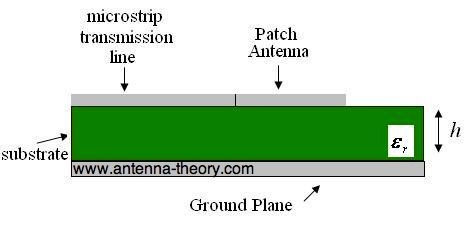
\includegraphics[width=0.4\linewidth]{ant/ant36.png}}
\caption{Geometría de microstrip.}
\end{figure}
Las antenas tipo parche poseen una tira conductora de largo \textit{L}, ancho \textit{W} y grosor \textit{T}. La tira conductora esta en la parte superior del substrato dieléctrico el cual tiene un ancho \textit{H}. En la parte inferior del substrato dieléctrico esta la tierra, como se ve en la figura.
donde:
\begin{itemize}
\item T y H z<<$\lambda$  ($\lambda$ es la longitud de onda en el espacio libre).
\item $\lambda$/3 <L< $\lambda$/2
\item 2.2 $\leq\epsilon_r\leq$ 12 (Se debe buscar la menor permitividad posible para lograr una mejor eficiencia de la antena).
\end{itemize}
Dependiendo de los requerimientos específicos para los cuales se construye una antena de microstrip de un solo elemento, se pueden recurrir a varios tipos de configuraciones los mas típicos son:
\begin{itemize}
\item Dipolo (tanto en su forma de media onda como de onda completa)
\item Cuadrada, rectangular, pentagonal, triangular, circular, disco con ranura, sector de disco, anillo, semi-disco, anillo elíptico, espiral.
\item Otro tipo particular de antena parche que ha surgido en años recientes es la llamada ``Antena  f  invertida plana'' muy utilizada para unidades móviles (es la mitad de una antena parche cuadrada).
\item Se pueden usar arreglos de antenas con el fin de lograr características deseadas 
\item El patrón de ondas de una antena parche es omnidireccional aunque la potencia radiada es emitida  solamente hacia la parte superior en su forma ideal.
\end{itemize}
\begin{figure}[]
\centering
\subfloat[Patrón de radiación 2D]{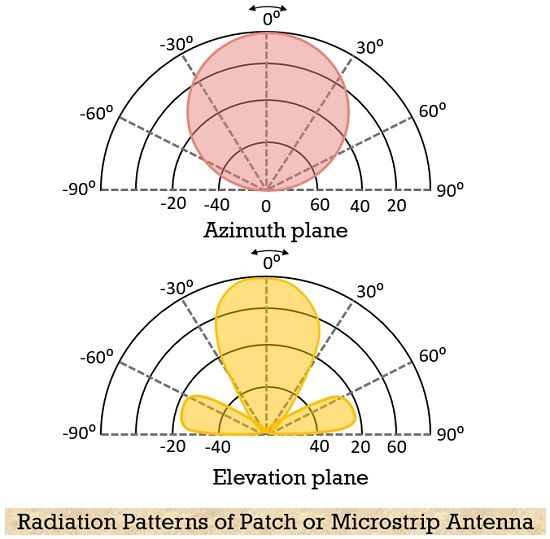
\includegraphics[width=0.4\linewidth]{ant/ant37.png}}
\subfloat[Patrón de radiación 3D]{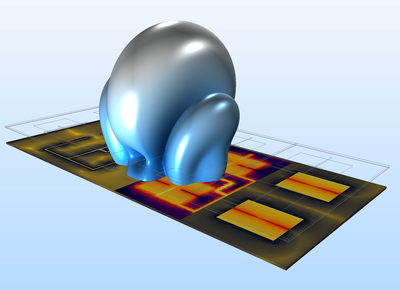
\includegraphics[width=0.4\linewidth]{ant/ant38.png}}
\caption{Patrón de radiación de una antena microstrip.}
\end{figure}
\subsection{Métodos de análisis}
Dependiendo de la sencillez y la precisión que se busque se puede seleccionar el método que mas se ajuste a las necesidades. Entre los diversos métodos para el análisis de antenas tipo parche se pueden mencionar:
\begin{itemize}
\item Modelos empíricos.
\item Modelos semi-empíricos.
\item Modelos de onda completa.
\end{itemize}
\subsubsection{Modelos empíricos}
Son los menos precisos a la hora de diseñar, su método de análisis se basa en la suposición de conceptos. Estos modelos pueden tener buen nivel de precisión cuando se trabajan en rango de frecuencias menores a los de las ondas milimétricas (f < 30GHz) pero si se salen de este rango el modelo comienza a tener graves imprecisiones por lo que es necesario usar otros modelos. Aquí se encuentra el modelo de línea de transmisión.\\
\textbf{Modelo líneas de transmisión}\\
Este modelo es el mas sencillo pero el mas impreciso además de que solamente puede ser utilizado para el diseño de antenas rectangulares y circulares. Este modelo considera los bordes de la antena como dos aperturas (slots) que radian.
Las aperturas a su vez son consideradas como admitancias complejas compuestas de una conductancia G y una susceptancia B, la siguiente figura muestra el circuito equivalente para una antena rectangular en el modelo de línea de transmisión.
\begin{figure}[H]
\centering
\includegraphics[width=0.6\linewidth]{ant/ant39.png}
\caption{Circuito antena rectangular.}
\end{figure}
\begin{definition}[Fringing Effects]
El efecto de franja (fringing effects) se debe a las líneas de campo eléctrico que hacen que el tamaño de la antena sea más ancho después de la excitación. La causa principal del efecto de franja se debe al ancho y la posición de la antena de alimentación. Los campos producidos por los fringing effects ayudan en la radiación y dan un patrón de radiación más directivo, pero la frecuencia de resonancia se desplaza de la frecuencia deseada.
\begin{center}
\includegraphics[width=0.7\linewidth]{ant/ant40.png}
\end{center}
\end{definition}
El modelo de línea de transmisión se resumen en los siguientes pasos:
\begin{enumerate}
\item Se especifica la frecuencia de operación y el sustrato a utilizar.
\item Se obtiene el ancho efectivo de la antena de parche rectangular mediante la formula:
\begin{displaymath}
W=\frac{1}{2f_r\sqrt{\mu_0\epsilon_0}}\sqrt{\frac{2}{\epsilon_r+1}}=\frac{c}{2f_r}\sqrt{\frac{2}{\epsilon_r+1}}
\end{displaymath}
\item Se obtiene la permitividad eléctrica efectiva mediante:
\begin{displaymath}
\epsilon_{ref}=\frac{\epsilon_r+1}{2}+\frac{\epsilon_r+1}{2}\corchetes{1+12\frac{h}{W}}^{-\frac{1}{2}}
\end{displaymath}
\item Se obtiene la extensión $\Delta L$ mediante la ecuación que se derivará en la obtención de la longitud real de la antena considerando la longitud efectiva.
\begin{displaymath}
\Delta L=0.412\cdot h\frac{\parentesis{\epsilon_{ref}+0.3}\parentesis{\frac{W}{h}+0.264}}{\parentesis{\epsilon_{ref}-0.258}\parentesis{\frac{W}{h}+0.8}}
\end{displaymath}
\item Longitud será:
\begin{displaymath}
L=\frac{1}{2\cdot f_r\sqrt{\epsilon_{ref}}\sqrt{\mu_0\epsilon_0}}-2\Delta L
\end{displaymath}
\end{enumerate}
\subsubsection{Modelo semi-empíricos}
Es un modelo mas complejo que el empírico pero menos preciso que el modelo de onda compleja. Ejemplos de este modelo se pueden nombrar los siguientes:
\begin{itemize}
\item Modelo de corriente superficial eléctrica.
\item Técnica de la transformada de Hankel.
\item Método de reciprocidad.
\item Enfoque de ecuación integral dual, etc.
\end{itemize}

\subsubsection{Modelos de onda completa}
Estos modelos se presentan como los mas precisos a la hora de diseñar, sin embargo también son los mas complicados de realizar y se requieren de herramientas computacionales avanzadas para llevar a cabo.
Como ejemplos de modelo de onda completa se tiene:
\begin{itemize}
\item Método de momentos en el dominio del tiempo.
\item Método de momentos en el dominio espectral.
\item Método de estados finitos.
\item Técnicas de transformada rápida de Fourier, etc.
\end{itemize}
\begin{notation}
Ejemplos de programas que usan el modelo de onda completa son el programa Sonnet y el programa HFSS. El software Sonnet usa el método de momentos, mientras que el software HFSS usa un método de elementos finitos modificado.
\end{notation}
\subsection{Alimentación}
Existen diferentes métodos para alimentar una antena microstrip de forma que radie lo mas eficientemente posible.
Por ejemplo esta el método de \textbf{alimentación por sonda coaxial} donde el pin de cable coaxial alimenta directamente al radiador, mientras que la parte negativa de este se conecta a la de tierra de la antena de microstrip.\\
Otro método de alimentación es el llamado \textbf{alimentación con Substrato de Guía de Onda Integrado} (Substrate Integrated Waveguide), con la que se tiene una antena (elemento radiador), en la parte superior de un substrato dieléctrico que recibe la alimentación de una guía de onda integrada en otro substrato dieléctrico localizada en la parte inferior de la antena. El acoplamiento electromagnético es através de una abertura localizada en la parte superior de la guía de onda y cuyas dimensiones y posicionamiento generan diferentes impedancias características y por lo tanto diferente acoplamiento como se muestra en la siguiente vista superior de la estructura para alimentar a la antena:
\begin{figure}[H]
\centering
\includegraphics[width=0.7\linewidth]{ant/ant41.png}
\caption{Formas de alimentación.}
\end{figure}
\section{Arreglo o arrays de antenas}
Un array es una antena compuesta por un número de radiadores idénticos ordenados regularmente y alimentados para obtener un diagrama de radiación predefinido.\\
Hay diferentes tipos de arrays. 
\begin{itemize}
\item Los arrays lineales tienen los elementos dispuestos sobre una línea.
\item Los arrays planos son agrupaciones bidimensionales cuyos elementos están sobre un plano.
\item Los arrays conformados tienen las antenas sobre una superficie
curva, como por ejemplo el fuselaje de un avión
\end{itemize}
Los arrays tienen la ventaja de que se puede controlar la amplitud de las corrientes y la fase de cada elemento, modificando la forma del diagrama de radiación. Además se puede conseguir que los parámetros de antena dependan de la señal recibida a través de circuitos asociados a los elementos radiantes, como en el caso de las agrupaciones adaptativas.\\
\begin{notation}
El factor de array es el diagrama de radiación de una agrupación de
elementos isotrópicos.
\end{notation}
Cuando los diagramas de radiación de cada elemento del array son iguales y los elementos están orientados en la misma dirección del espacio, el diagrama de radiación de la agrupación se puede obtener como el producto del factor de array por el diagrama de radiación del elemento.\\
Hay 5 métodos para controlar el diagrama de radiación de un array:
\begin{enumerate}
\item Mediante la configuración geométrica (linear, rectangular, circular…)
\item La situación relativa de los elementos
\item La amplitud de la excitación de cada elemento
\item La fase de la excitación de cada elemento
\item El diagrama de radiación de cada elemento
\end{enumerate}
\subsection{Arrays lineales}
Dos radiadores iguales, alimentados con misma amplitud y fase. Ambos radiadores producen ondas esféricas que se sumarán de forma
constructiva en determinadas direcciones y cancelación en otras
%imagen
En el caso de que estemos suficientemente lejos de las fuentes, y suponiendo que el primer radiador se encuentra en el origen de coordenadas, la diferencia de caminos recorrida por ambas ondas será:
\begin{equation}
R_1-R_2=d\cdot\cos\theta
\end{equation}
Se podrá escribir la amplitud total de la señal como el producto de una onda esférica por un factor de interferencia.
\begin{equation}
\frac{e^{-jkr}}{4\pi\cdot r}\parentesis{1+e^{jkd\cos\theta}}
\end{equation}
Se producirá \textbf{interferencia constructiva} cuando la diferencia de caminos sea un \textbf{múltiplo entero de longitudes de onda}, siendo la amplitud de la señal el doble. Cuando la diferencia de fase sea un\textbf{ múltiplo impar de $\pi$}, la interferencia será destructiva.
\begin{tabular}{k{0.5\linewidth}  j{0.5\linewidth}}
        \includegraphics[width=0.7\linewidth]{ant/ant42.png} & \textbf{d=0}\newline Si la separación entre los dos
radiadores es cero, no existirá
ningún tipo de desfase, por lo que
la señal se radiará isotrópicamente
en todas las direcciones del
espacio. \\
        \includegraphics[width=0.7\linewidth]{ant/ant43.png} & \textbf{d=$\lambda/2$}\newline Si los dos elementos están separados una semilongitud de onda, se
producirá un máximo en la dirección perpendicular a la recta que
une sus posiciones, obteniendo un nulo de radiación en la dirección
de dicho eje, ya que las señales se sumarán en oposición de fase.\\
        \includegraphics[width=0.7\linewidth]{ant/ant44.png} & \textbf{d=$\lambda$}\newline Si la separación entre los dos radiadores es de una longitud de onda
se producirán máximos de radiación en las direcciones del eje y
perpendiculares a él, produciéndose cancelación para un ángulo en
el que ambas señales esté en oposición de fase, lo que sucede para la
dirección que forma un ángulo de 60° con el eje de la agrupación. \\
        \includegraphics[width=0.7\linewidth]{ant/ant45.png} & \textbf{d=$\lambda/4$}\newline Cuando la diferencia de fases es de $-\pi/4$ y la separación es $\lambda/4$, las
ondas se suman en la dirección del eje z en fase, y en –z en oposición
de fase. 
\end{tabular}
\begin{figure}[H]
\centering
\includegraphics[width=\linewidth]{ant/ant46.png}
\caption{Diagramas tridimensionales de dos radiadores isotrópicos de la misma amplitud, en función de
la separación \textit{d} y de la diferencia de fases $\alpha$.}
\end{figure}
%----------------------------------------------------------------------------------------
%	NEW CHAPTER
%----------------------------------------------------------------------------------------
\part{Internetworking 2}
\chapterimage{chapter_head_IT2.pdf} % Chapter heading image

\chapter{Unidad I}
\section{Protocolo spanning tree}\index{Protocolo spanning tree}
Las redes conmutadas, por lo general, tienen rutas  redundantes y enlaces redundantes incluso entre los  mismos dos dispositivos. Las rutas redundantes eliminan un punto de falla único  para mejorar la confiabilidad y disponibilidad. Las rutas redundantes pueden causar bucles de capa 2  físicos y lógicos.
\begin{figure}[H]
\centering
\includegraphics[width=0.6\linewidth]{IN2/IN1.png}
\caption{Camino redundante de PC1 a PC4 en caso falle una ruta.}
\end{figure}
El algoritmo \textbf{Spanning Tree} (árbol de expansión) se utiliza en los switches para prevenir los bucles lógicos que pueden aparecer en una red. Los bucles se producen cuando existen varios caminos distintos entre dos puntos de la red y su efecto es que las tramas pueden circular de forma indefinida atrapadas en un bucle sin conseguir alcanzar su destino, lo que además afectará negativamente al rendimiento de la red. El algoritmo \textit{Spanning Tree} ayuda a los switches a elegir el camino más idóneo y, por tanto, elimina los bucles.
\begin{notation}
El protocolo \textit{spanning tree esta detallado especificado en el estándar \textbf{IEEE 802.1D}. Existe su variante con funcionamiento optimizado: \textbf{spanning tree rápido}-IEEE 802.1w}
\end{notation}
\subsection{Problemas con la redundancia de capa 1}
Los problemas con los bucles son:
\begin{itemize}
\item \textbf{Inestabilidad de la base de datos MAC}: Las tramas de ethernet no poseen Tiempo de duración, como el encabezado IP de capa 3. Esto significa que Ethernet no tiene ni un mecanismo para descartar las tramas que se propagan innecesariamente. EL bucle empieza de la siguiente manera; observando la imagen  \ref{fig:inestabilidad spanning tree}:
\begin{enumerate}
\item PC1 envía un marco de transmisión a S2. S2 recibe el marco de transmisión en F0/11. Cuando S2 recibe la trama de transmisión, actualiza su tabla de direcciones MAC para registrar que la PC1 está disponible en el puerto F0/11.
\item Debido a que es una trama de transmisión, S2 reenvía la trama por todos los puertos, incluidos Trunk1 y Trunk2. Cuando la trama de transmisión llega a S3 y S1, los switches actualizan sus tablas de direcciones MAC para indicar que PC1 está disponible en el puerto F0/1 en S1 y en el puerto F0/2 en S3.
\item Debido a que es una trama de transmisión, S3 y S1 reenvían la trama por todos los puertos excepto el puerto de entrada. S3 envía el marco de transmisión de PC1 a S1. S1 envía el marco de transmisión de PC1 a S3. Cada conmutador actualiza su tabla de direcciones MAC con el puerto incorrecto para PC1.
\item Cada conmutador reenvía la trama de difusión por todos sus puertos excepto el puerto de entrada, lo que hace que ambos conmutadores reenvíen la trama a S2.
\item Cuando S2 recibe las tramas de transmisión de S3 y S1, la tabla de direcciones MAC se actualiza con la última entrada recibida de los otros dos conmutadores.
\item S2 reenvía la trama de transmisión por todos los puertos excepto el último puerto recibido. El ciclo comienza de nuevo.
\end{enumerate}
\begin{figure}[H]
\centering
\includegraphics[width=0.6\linewidth]{IN2/IN2.png}
\caption{Momento 6 del bucle.}
\label{fig:inestabilidad spanning tree}
\end{figure}
Debido a los cambios constantes en la tabla de direcciones MAC, los switches S3  y S1 no saben a qué puerto reenviar las tramas.
\item \textbf{Tormenta de difusión}: Si no controlamos el problema anterior, las demás computadoras también deben mandar primero sus marcos de transmisión, y el problema de inestabilidad se acrecentará, esto se refleja en el sistema como varios tramas de transmisión \textbf{atrapados} en la red, \textbf{consumiendo ancho de banda} y hasta saturándola. Haciendo que sea imposible el envío de datos legítimos de comunicación. Si no hay ancho de banda útil para el envío de información, la red no estará disponible causando una denegación de servicio efectiva (DoS).\\
Hay otras consecuencias de las tormentas de transmisión. Debido a que el tráfico de difusión se reenvía a todos los puertos de un conmutador, todos los dispositivos conectados tienen que procesar todo el tráfico de difusión que se inunda sin cesar alrededor de la red en bucle. Esto puede hacer que el dispositivo final no funcione correctamente debido a los requisitos de procesamiento necesarios para soportar una carga de tráfico tan alta en la NIC.\\
Secuencia de eventos:
\begin{enumerate}
\item PC1 envía una trama de transmisión a la red en bucle (Inestabilidad en la base de datos MAC).
\item La trama de transmisión se repite entre todos los conmutadores interconectados en la red.
\item La PC4 también envía una trama de transmisión a la red en bucle.
\item La trama de transmisión PC4 queda atrapada en el bucle entre todos los conmutadores interconectados, al igual que la trama de transmisión PC1.
\item A medida que más dispositivos envían transmisiones a través de la red, más tráfico queda atrapado en el bucle y consume recursos. Esto eventualmente crea una tormenta de transmisión que hace que la red falle.
\item Cuando la red está totalmente saturada con el tráfico de difusión que circula entre los conmutadores, el conmutador descarta el tráfico nuevo porque no puede procesarlo. La Figura \ref{fig:tormenta de difusión} muestra la tormenta de difusión resultante.
\end{enumerate}
\begin{figure}[H]
\centering
\includegraphics[width=0.6\linewidth]{IN2/IN3.png}
\caption{Tormenta de difusión}
\label{fig:tormenta de difusión}
\end{figure}
Una tormenta de transmisión puede desarrollarse en segundos porque los dispositivos conectados a una red envían regularmente tramas de transmisión, como solicitudes ARP. Como resultado, cuando se crea un bucle, la red conmutada se desconecta rápidamente.
\item \textbf{Tramas de unidifusión duplicadas}: Una trama de unidifusión desconocida se produce  cuando el switch no tiene la dirección MAC de destino en la tabla de direcciones MAC y debe difundir la trama a todos los puertos, excepto el  puerto en que se recibió la trama (puerto de ingreso). Si se envían tramas de unidifusión desconocidas a  una red con bucles, se puede producir la llegada de  tramas duplicadas al dispositivo de destino.\\
Secuencia de eventos:
\begin{enumerate}
\item PC1 envía una trama de unidifusión destinada a PC4.
\item S2 no tiene una entrada para PC4 en su tabla MAC. En un intento por encontrar la PC4, inunda la trama de unidifusión desconocida de todos los puertos del switch excepto el puerto que recibió el tráfico.
\item La trama llega a los conmutadores S1 y S3.
\item S1 tiene una entrada de dirección MAC para PC4, por lo que reenvía la trama a PC4.
\item S3 tiene una entrada en su tabla de direcciones MAC para PC4, por lo que reenvía la trama de unidifusión de Trunk3 a S1.
\item S1 recibe la trama duplicada y la reenvía a la PC4.
\item PC4 ahora ha recibido el mismo marco dos veces.
\end{enumerate}
\begin{figure}[H]
\centering
\includegraphics[width=0.6\linewidth]{IN2/IN4.png}
\caption{S1 y S3 envian una trama duplicada a la PC4.}
\end{figure}
\end{itemize}
\section{Tecnología EtherChannel}
\subsection{Funcionamiento}
Hay escenarios en los que se necesita más ancho de banda o redundancia entre  dispositivos que lo que puede proporcionar un único enlace. Se pueden conectar varios  enlaces entre dispositivos para aumentar el ancho de banda. Sin embargo, el protocolo de  árbol de expansión (STP), que está habilitado en dispositivos de \textbf{capa 2} como switches. Cisco de forma predeterminada, bloqueará enlaces redundantes para evitar bucles de  conmutación. Se necesita una tecnología de agregación de enlaces que permita \textbf{vínculos redundantes} entre dispositivos que \textbf{no serán bloqueados por STP}. Esa tecnología se conoce como EtherChannel.\\
EtherChannel es una tecnología de agregación de enlaces que \textbf{agrupa} varios enlaces físicos Ethernet en un único enlace lógico. Se utiliza para proporcionar tolerancia a fallos, uso compartido de carga, mayor ancho de banda y redundancia entre switches, routers y servidores. La tecnología de EtherChannel hace posible combinar la cantidad de enlaces físicos entre los switches para aumentar la velocidad general de la comunicación switch a switch.\\
En los inicios, Cisco desarrolló la  tecnología EtherChannel como una técnica switch a switch LAN  para \textbf{agrupar} varios puertos Fast  Ethernet o gigabit Ethernet en un  único canal lógico. Cuando se configura un EtherChannel, la interfaz virtual  resultante se denomina ``canal de  puertos'' (\textit{port channel}). Las interfaces físicas se agrupan en una interfaz de canal  de puertos, como se muestra en la figura \ref{fig:tec ether}.
\begin{figure}[H]
\centering
\includegraphics[width=0.6\linewidth]{IN2/IN5.png}
\caption{Tecnología EtherChannel}
\label{fig:tec ether}
\end{figure}
\subsection{Ventajas de EtherChannel}
\begin{itemize}
\item La mayoría de las tareas de configuración se pueden realizar en la interfaz EtherChannel en lugar  de en cada puerto individual, lo que asegura la coherencia de configuración en todos los enlaces.
\item EtherChannel depende de los puertos de switch existentes. No es necesario actualizar el enlace a  una conexión más rápida y más costosa para tener más ancho de banda.
\item El equilibrio de carga ocurre entre los enlaces que forman parte del mismo EtherChannel.
\item EtherChannel crea una agregación que se ve como un único enlace lógico. Cuando existen varios  grupos EtherChannel entre dos switches, STP puede bloquear uno de los grupos para evitar los  bucles de switching. Cuando STP bloquea uno de los enlaces redundantes, bloquea el  EtherChannel completo. Esto bloquea todos los puertos que pertenecen a ese enlace  EtherChannel. Donde solo existe un único enlace EtherChannel, todos los enlaces físicos en el  EtherChannel están activos, ya que STP solo ve un único enlace (lógico).
\item EtherChannel proporciona redundancia, ya que el enlace general se ve como una única conexión  lógica. Además, la pérdida de un enlace físico dentro del canal no crea ningún cambio en la  topología.
\end{itemize}
\subsection{Restricciones}
\begin{itemize}
\item No pueden mezclarse los tipos de interfaz. Por ejemplo, Fast Ethernet y Gigabit Ethernet no se pueden mezclar dentro de un único EtherChannel.
\item En la actualidad, cada EtherChannel puede constar de hasta ocho puertos Ethernet configurados  de manera compatible. El EtherChannel proporciona un ancho de banda full-duplex de hasta 800  Mbps (Fast EtherChannel) u 8 Gbps (Gigabit EtherChannel) entre un switch y otro switch o host.
\item El switch Cisco Catalyst 2960 Layer 2 soporta actualmente hasta seis EtherChannels.
\item La configuración de los puertos individuales que forman parte del grupo EtherChannel debe ser  coherente en ambos dispositivos. Si los puertos físicos de un lado se configuran como enlaces  troncales, los puertos físicos del otro lado también se deben configurar como enlaces troncales  dentro de la misma VLAN nativa. Además, todos los puertos en cada enlace EtherChannel se  deben configurar como puertos de capa 2.
\item Cada EtherChannel tiene una interfaz de canal de puertos lógica, la configuración aplicada a la  interfaz de canal de puertos afecta a todas las interfaces físicas que se asignan a esa interfaz.
\end{itemize}
\subsection*{Protocolos de negociación automática}
Los EtherChannels se pueden formar por medio de una negociación con uno de dos  protocolos: Port Aggregation Protocol (PAgP) o Link Aggregation Control Protocol (LACP).  Estos protocolos permiten que los puertos con características similares formen un canal  mediante una negociación dinámica con los switches adyacentes.
\subsection{Funcionamiento del PAgP}
PAgP (pronunciado ``Pag - P'') es un protocolo patentado por Cisco que ayuda en la creación  automática de enlaces EtherChannel. Cuando se configura un enlace EtherChannel mediante PAgP,  se envían paquetes PAgP entre los puertos aptos para EtherChannel para negociar la formación de un  canal. Cuando PAgP identifica enlaces Ethernet compatibles, agrupa los enlaces en un EtherChannel.  El EtherChannel después se agrega al árbol de expansión como un único puerto.\\
Cuando se habilita, PAgP también administra el EtherChannel. Los paquetes PAgP se envían cada 30  segundos. PAgP revisa la coherencia de la configuración y administra los enlaces que se agregan, así  como las fallas entre dos switches. Cuando se crea un EtherChannel, asegura que todos los puertos  tengan el mismo tipo de configuración.
\begin{notation}
En EtherChannel, es obligatorio que todos los puertos tengan la misma velocidad, la misma  configuración de dúplex y la misma información de VLAN. Cualquier modificación de los puertos  después de la creación del canal también modifica a los demás puertos del canal.
\end{notation}
\subsection{PAgP}\index{PAgP}
PAgP ayuda a crear el enlace EtherChannel al detectar la configuración de cada lado y asegurarse de que los enlaces sean  compatibles, de modo que se pueda habilitar el enlace EtherChannel cuando sea necesario. Los modos de PAgP de la siguiente  manera:
\begin{itemize}
\item \textbf{Encendido}: Este modo obliga a la interfaz a proporcionar un canal sin PAgP. Las interfaces configuradas en el modo encendido no intercambian paquetes PAgP.
\item \textbf{PAgP desirable}: Este modo PAgP coloca una interfaz en un estado de negociación activa en el que la interfaz inicia negociaciones con otras interfaces al enviar paquetes PAgP.
\item \textbf{PAgP auto}: Este modo PAgP coloca una interfaz en un estado de negociación pasiva en el que la interfaz responde a los paquetes PAgP que recibe, pero no inicia la negociación PAgP.
\end{itemize}
Los modos deben ser compatibles en cada lado. Si se configura un lado en modo automático, se coloca en estado pasivo, a la  espera de que el otro lado inicie la negociación del EtherChannel. Si el otro lado se establece en modo automático, la  negociación nunca se inicia y no se forma el canal EtherChannel. Si se deshabilitan todos los modos mediante el comando \textit{\textbf{no}} o  si no se configura ningún modo, entonces se deshabilita el EtherChannel. El modo \textit{encendido} coloca manualmente la interfaz en  un EtherChannel, sin ninguna negociación. Funciona solo si el otro lado también se establece en modo encendido. Si el otro lado  se establece para negociar los parámetros a través de PAgP, no se forma ningún EtherChannel, ya que el lado que se establece  en modo \textit{encendido} no negocia. El hecho de que no haya negociación entre los dos switches significa que no hay un control, para asegurarse de que todos los enlaces en el EtherChannel terminen del otro lado o de que haya compatibilidad con PAgP en  el otro switch.
\begin{table}[H]
\centering
\begin{tabular}{|c|c|c|}
\hline
\rowcolor[HTML]{9698ED} 
S1        & S2             & Establecmiento del canal \\ \hline
On        & On             & Sí                       \\ \hline
On        & Desirable/Auto & No                       \\ \hline
Desirable & Desirable      & Sí                       \\ \hline
Desirable & Auto           & Sí                       \\ \hline
Auto      & Desirable      & Sí                       \\ \hline
Auto      & Auto           & No                       \\ \hline
\end{tabular}
\caption{Combinacion PAgP y el resultado del establecimiento.}
\end{table}
\subsection{LACP}\index{LACP}
LACP forma parte de una especificación \textbf{IEEE (802.3ad)} que permite agrupar varios puertos físicos  para formar un único canal lógico. LACP permite que un switch negocie un grupo automático mediante  el envío de paquetes LACP al otro switch. Realiza una función similar a PAgP con EtherChannel de  Cisco. Debido a que LACP es un estándar IEEE, se puede usar para facilitar los EtherChannels en entornos de varios proveedores. En los dispositivos de Cisco, se admiten ambos protocolos.\\
LACP proporciona los mismos beneficios de negociación que PAgP. LACP ayuda a crear el enlace  EtherChannel al detectar la configuración de cada lado y al asegurarse de que sean compatibles, de  modo que se pueda habilitar el enlace EtherChannel cuando sea necesario. Los modos para LACP  son los siguientes:
\begin{itemize}
\item \textbf{On}: Este modo obliga a la interfaz a proporcionar un canal sin LACP. Las interfaces
configuradas en el modo encendido no intercambian paquetes LACP.
\item \textbf{LACP active}: Este modo de LACP coloca un puerto en estado de negociación activa. En este
estado, el puerto inicia negociaciones con otros puertos mediante el envío de paquetes LACP.
\item \textbf{LACP passive}: Este modo de LACP coloca un puerto en estado de negociación pasiva. En este  estado, el puerto responde a los paquetes LACP que recibe, pero no inicia la negociación de  paquetes LACP.
\end{itemize}
\begin{table}[H]
\centering
\begin{tabular}{|c|c|c|}
\hline
\rowcolor[HTML]{9698ED} 
S1      & S2             & Establecmiento del canal \\ \hline
On      & On             & Sí                       \\ \hline
On      & Active/Passive & No                       \\ \hline
Active  & Active         & Sí                       \\ \hline
Active  & Passive        & Sí                       \\ \hline
Passive & Active         & Sí                       \\ \hline
Passive & Passive        & No                       \\ \hline
\end{tabular}
\caption{Diversas combinaciones de modos LACP en S1 y S2 y el resultado resultante del establecimiento de canales.}
\end{table}
\subsection{Pautas y restricciones para la configuración}
\begin{itemize}
\item \textbf{EtherChannel support}: Todas las interfaces Ethernet deben admitir EtherChannel,
sin necesidad de que las interfaces sean físicamente contiguas
\item \textbf{Speed and duplex}: Configure todas las interfaces en un EtherChannel para que  funcionen a la misma velocidad y en el mismo modo dúplex.
\item \textbf{VLAN match}: Todas las interfaces en el grupo EtherChannel se deben asignar a la  misma VLAN o se deben configurar como enlace troncal (mostrado en la figura).
\item \textbf{Rango de VLAN}: Un EtherChannel admite el mismo rango permitido de VLAN en  todas las interfaces de un EtherChannel de enlace troncal. Si el rango permitido de  VLAN no es el mismo, las interfaces no forman un EtherChannel, incluso si se  establecen en modo auto o desirable .
\end{itemize}
\section{Conceptos de routing}
El routing es la capacidad de buscar la ruta correcta para mover o transferir paquetes de información entre una o varias redes de Internet. Para hacer routing se necesitan de routers, estos son computadoras especializadas que poseen componentes como:
\begin{itemize}
\item Unidad central de procesamiento (CPU)
\item Sistema operativo (OS): los routers utilizan IOS de Cisco
\item Memoria y almacenamiento (RAM, ROM, NVRAM, flash, disco duro)
\item Tarjetas de interfaz de red
\end{itemize}
Estos se pueden enlazar mediante puertos para interconectarse con otras redes.
\begin{figure}[H]
\centering
\includegraphics[width=0.6\linewidth]{IN2/IN6.png}
\caption{Memorias del router}
\end{figure}
Más adelante se estudiará las ruta estática y los protocolos de routing dinámico para descubrir redes remotas y crear sus tablas de routing. La tabla de routing ayuda a determinar la mejor ruta para enviar paquetes. Los paquetes son encapsulados y se envían en cada interfaz indicada en la tabla de routing.
\begin{figure}
\centering
\includegraphics[width=\linewidth]{IN2/IN7.png}
\caption{Encapsulación de paquetes.}
\end{figure}
\subsection{Funciones de routing}
\begin{itemize}
\item \textbf{Conectar redes y administrar el tráfico de ellas}: El router es el responsable del routing, capacidad de reenviar paquetes IP desde una red a otra, del tráfico entre redes. Los routers encapsulan los paquetes y los reenvían a la interfaz indicada en la tabla de routing. Los métodos de reenvío de paquetes son:
\begin{itemize}
	\item Switching de procesos: es  un mecanismo de reenvío de  paquetes más antiguo que  todavía está disponible para  routers Cisco.
	\item Switching rápido: es un  mecanismo común de reenvío  de paquetes que usa una  memoria caché de switching  rápido para almacenar la información de siguiente salto.
	\item Cisco Express Forwarding: Es el mecanismo más reciente, más rápido y más utilizado de CISCO.
\end{itemize}
\item \textbf{Aceleración de datos entre redes}: Los routers son capaces de utilizar las tablas de routing para determinar cuál es la mejor ruta para enviar paquetes. Pueden emplear rutas estáticas o dinámicas para descubrir redes remotas.
\item \textbf{Creación de tabla de routing}: La tabla de routing es el listado de todas las posibles rutas de la red. Cuando un router recibe paquetes IP que deben enviarse a otro lugar de la red, mira la dirección IP de destino del paquete y, luego, busca la información de routing en la tabla de routing.
\item \textbf{Seguridad de red}: El router sirve como un firewall, lo que restringe el acceso de cualquier persona que no esté autorizada. Esto se hace con claves de seguridad similares a las contraseñas, sólo los dispositivos precargados con la clave de seguridad o usadas por usuarios que pueden ingresar la contraseña correcta, tienen acceso a la red
\end{itemize}
\subsection{Conexión de dispositivos}
Para conectar los dispositivos en los routers se debe hacer uso de:
\begin{itemize}
\item \textbf{Gateways predeterminadas}: Para habilitar el acceso a  la red, los dispositivos deben estar configurados con la siguiente información de  direcciones IP.
\begin{itemize}
\item \textbf{Dirección IP}: Identifica a un  host único en una red local.
\item \textbf{Máscara de subred}: Identifica a la subred de la  red del host.
\item \textbf{Gateway predeterminado}: Identifica al router al que se  envía un paquete cuando el  destino no está en la misma  subred de la red local.
\end{itemize}
\item \textbf{Habilitar IP en un host}: La dirección IP puede ser asignada en forma estática o dinámica.
\begin{itemize}
\item Estática: Manualmente. Al host se le asigna  manualmente una dirección IP, una máscara de subred y un gateway  predeterminado. También se puede asignar la dirección IP de un  servidor DNS. Se utiliza para identificar recursos de red específicos, como servidores de red e impresoras. Se puede utilizar en redes muy pequeñas con pocos hosts.
\item Dinámica: Un servidor asigna en forma dinámica la información de la dirección IP utilizando el \textbf{ protocolo de  configuración dinámica de hosts} (DHCP). La mayoría de los hosts obtienen la información de su dirección IP  mediante DHCP. Los routers Cisco pueden proporcionar servicios DHCP.
\end{itemize}
\item \textbf{Acceso a la consola}: 
\begin{itemize}
\item Puerto de computadora: Puerto serie y puerto USB tipo A
\item Cable requerido: Cable de consola, Adaptador de puerto serie USB a RS232 y Cable USB tipo A a USB tipo B.
\item Puerto en el ISR: Puerto de consola RJ-45 y Puerto de consola USB Tipo B
\item Emulación del terminal: Tera Term o PuTTY.
\end{itemize}
\item \textbf{Habilitar IP en in switch}
\end{itemize}
\subsection{Verificación de la conectividad de redes conectadas directamente}
Existen diferentes métodos para comprobar la conectividad entre dos redes conectadas:
\subsubsection{Prueba de stack}
\begin{enumerate}
\item \textbf{PING}: El comando ping es una manera efectiva de probar la conectividad. La prueba se denomina prueba de stack de protocolos, porque el comando ping se mueve desde la Capa 3 del Modelo OSI hasta la Capa 2 y luego hacia a la Capa. El ping utiliza el protocolo ICMP (Protocolo de mensajes de control de Internet) para comprobar la conectividad.
\item \textbf{Indicadores de ping IOS}: Un ping de IOS cederá a una de varias indicaciones para cada eco ICMP enviado. Los indicadores más comunes son:
! - indica la recepción de una respuesta de eco ICMP
. - indica un límite de tiempo cuando se espera una respuesta
U - se recibió un mensaje ICMP inalcanzable
\item \textbf{Prueba de loopback}: A modo de primer paso en la secuencia de prueba, se utiliza el comando ping para verificar la configuración IP interna en el host local. Recuerde que esta prueba se cumple con el comando ping en una dirección reservada denominada loopback (127.0.0.1). Esto verifica la correcta operación del stack de protocolos desde la capa de Red a la capa Física, y viceversa, sin colocar realmente una señal en el medio.
\end{enumerate}
\subsubsection{Asignación de interfaz}
Del mismo modo que se usan comandos y utilidades para verificar la configuración de un host, se deben aprender los comandos para verificar las interfaces de dispositivos intermediarios. El IOS provee comandos para verificar la operación de interfaces de router y switch.
\begin{enumerate}
\item \textbf{Verificación de interfaz de router}: Uno de los comandos más utilizados es el comando show ip interface brief. Este proporciona un resultado más abreviado que el comando show ip interface. Ofrece además un resumen de la información clave de todas las interfaces.
\item \textbf{Prueba red local}: La siguiente prueba de la secuencia corresponde a los hosts en la LAN local. Al hacer ping a los hosts remotos satisfactoriamente se verifica que tanto el host local (en este caso, el router) como el host remoto estén configurados correctamente. Esta prueba se realiza al hacer ping a cada host en forma individual en la LAN. Si un host responde con el mensaje "Destination Unreachable" (destino inalcanzable), observe qué dirección no fue satisfactoria y continúe haciendo ping a los otros hosts de la LAN. Otro mensaje de falla es "Request Timed Out" (la petición ha expirado). Indica que no hubo respuesta al intento del ping en el período de tiempo predeterminado, lo cual indica que el problema puede estar en la latencia de red.
\end{enumerate}
\subsection{Determinación de ruta}
\subsubsection{Función determinación de ruta}
La función de determinación de ruta es el proceso según el cual el router determina qué ruta usar cuando envía un paquete. Para determinar la mejor ruta, el router \textbf{busca} en su tabla de enrutamiento una dirección de red que coincida con la dirección IP de destino del paquete. El resultado de esta búsqueda es una de tres determinaciones de ruta:
\begin{itemize}
\item \textbf{Red conectada directamente}: si la dirección IP de destino del paquete pertenece a un dispositivo en una red que está directamente conectado a una de las interfaces del router, ese paquete se envía directamente a ese dispositivo. Esto significa que la dirección IP de destino del paquete es una dirección host en la misma red que la interfaz de este router.
\item \textbf{Red remota}: si la dirección IP de destino del paquete pertenece a una red remota, entonces el paquete se envía a otro router. Las redes remotas sólo se pueden alcanzar mediante el envío de paquetes a otro router.
\item \textbf{Sin determinación de ruta}: si la dirección IP de destino del paquete no pertenece ya sea a una red conectada o remota, y si el router no tiene una ruta por defecto, entonces el paquete se descarta. El router envía un mensaje ICMP de destino inalcanzable a la dirección IP de origen del paquete. En los primeros dos resultados, el router vuelve a encapsular el paquete IP en el formato de la trama de enlace de datos de Capa 2 de la interfaz de salida. El tipo de interfaz determina el tipo de encapsulación de Capa 2. Por ejemplo, si la interfaz de salida es FastEthernet, el paquete se encapsula en una trama de Ethernet. Si la interfaz de salida es una interfaz serial configurada para PPP, el paquete IP se encapsula en una trama PPP.
\end{itemize}
\subsubsection{Función de conmutación}
La función de conmutación es el proceso utilizado por un router para \textbf{aceptar} un paquete en una interfaz y \textbf{enviarlo} desde otra interfaz. Una responsabilidad clave de la función de conmutación es la de \textbf{encapsular} los paquetes en el tipo de trama de enlace de datos correcto para el enlace de datos de salida.
\section{Routing estático}
\begin{figure}[H]
\centering
\includegraphics[width=0.7\linewidth]{IN2/IN8.png}
\caption{Sintaxis comando \textit{IP route}.}
\end{figure}
El enrutamiento estático proporciona un método que otorga a los ingenieros de redes \textbf{control absoluto} sobre las rutas por las que se transmiten los datos en una internetwork. Para adquirir este control, en lugar de configurar protocolos de enrutamiento dinámico para que creen las tablas de enrutamiento, se crean manualmente. Es importante entender las ventajas y desventajas de la implementación de rutas estáticas, porque se utilizan extensamente en internetworks pequeñas y para establecer la conectividad con proveedores de servicios. Es posible que se crea que el enrutamiento estático es sólo un método antiguo de enrutamiento y que el enrutamiento dinámico es el único método usado en la actualidad. Esto no es así, además, se destaca que escribir una ruta estática en un router no es más que especificar una ruta y un destino en la tabla de enrutamiento, y que los protocolos de enrutamiento hacen lo mismo, sólo que de manera automática. Sólo hay dos maneras de completar una tabla de enrutamiento: manualmente (el administrador agrega rutas estáticas) y automáticamente (por medio de protocolos de enrutamiento dinámico). 
\begin{itemize}
\item Facilita el mantenimiento de la tabla de enrutamiento en redes más pequeñas en las cuales no está previsto que crezcan significativamente.
\item Proporciona routing hacia las redes de rutas internas y desde estas. Una red de rutas internas es aquella a la cual se accede a través de una única ruta y cuyo router tiene solo un vecino.
\item Utiliza una única ruta predeterminada para representar una ruta hacia cualquier red que no tenga una coincidencia más específica con otra ruta en la tabla de routing.
\end{itemize}
\subsection{Tipos de rutas estáticas}
Las rutas estáticas suelen usarse con más frecuencia para conectarse a una red específica o para proporcionar un gateway de último recurso para una red de rutas internas. También pueden utilizarse para lo siguiente:
\begin{itemize}
\item Para reducir el número de rutas anunciadas mediante el resumen de varias redes contiguas como una sola ruta estática
\item Para crear una ruta de respaldo en caso de que falle un enlace de la ruta principal
\end{itemize}
\subsubsection*{Ruta estática predeterminada}
IPv4 e IPv6 admiten la configuración de rutas estáticas. Las rutas estáticas son útiles para conectarse a una red remota específica.
\subsubsection*{Ruta estática predeterminada}
Una ruta por defecto o predeterminada, es una ruta que coincide con \textbf{todos los paquetes} y es utilizada por el router si un paquete no coincide con ninguna otra ruta más específica en la tabla de routing. Además, puede ser aprendida de forma dinámica o configurada de manera estática. Una ruta estática predeterminada es simplemente una ruta estática con \textbf{0.0.0.0/0} como dirección IPv4 de destino. Al configurar una ruta estática predeterminada, se crea un gateway de último recurso. Las rutas estáticas predeterminadas se utilizan en los siguientes casos:
\begin{itemize}
\item Cuando ninguna otra ruta de la tabla de routing coincide con la dirección IP destino del paquete. En otras palabras, cuando no existe una coincidencia más específica. Se utilizan comúnmente cuando se conecta un router periférico de una compañía a la red ISP.
\item Cuando un router tiene otro router único al que está conectado. En esta situación, se conoce al router como router de rutas internas.
\end{itemize}
\subsubsection*{Rutas estática resumida}
Para reducir el número de entradas en la tabla de routing, se pueden resumir varias rutas estáticas en una única ruta estática si se presentan las siguientes condiciones:
\begin{itemize}
\item Las redes de destino son contiguas y se pueden resumir en una única dirección de red.
\item Todas las rutas estáticas utilizan la misma interfaz de salida o la dirección IP del siguiente salto.
\end{itemize}
\subsubsection*{Ruta estática flotante}
Las rutas estáticas flotantes son rutas estáticas que se utilizan para proporcionar una ruta de \textbf{respaldo} a una ruta estática o dinámica principal, en el caso de una falla del enlace. La ruta estática flotante se utiliza únicamente cuando la ruta principal \textbf{no está disponible}. Para lograrlo, la ruta estática flotante se configura con una distancia administrativa mayor que la ruta principal. La distancia administrativa representa la \textbf{confiabilidad} de una ruta. Si existen varias rutas al destino, el router elegirá la que tenga una menor distancia administrativa. Por ejemplo, suponga que un administrador desea crear una ruta estática flotante como respaldo de una ruta descubierta por EIGRP. La ruta estática flotante se debe configurar con una \textbf{distancia administrativa mayor} que el EIGRP. El EIGRP tiene una distancia administrativa de 90. Si la ruta estática flotante se configura con una distancia administrativa de 95, se prefiere la ruta dinámica descubierta por el EIGRP a la ruta estática flotante. Si se pierde la ruta descubierta por el EIGRP, en su lugar se utiliza la ruta estática flotante.
\begin{figure}[H]
\centering
\includegraphics[width=0.8\linewidth]{IN2/IN9.png}
\caption{Ruta estática flotante.}
\end{figure}
\section{Routing dinámico}
Los protocolos de enrutamiento mantienen tablas de enrutamiento dinámicas por medio de mensajes de actualización del enrutamiento, que contienen información acerca de los cambios sufridos en la red, y que indican al software del router que actualice la tabla de enrutamiento en consecuencia. Intentar utilizar el enrutamiento dinámico sobre situaciones que no lo requieren es una pérdida de ancho de banda, esfuerzo, y en consecuencia de dinero. 
\subsection{Comparación entre routing dinámico y estático}
\textbf{Routing estático}
\begin{enumerate}
\item Facilita el mantenimiento de la tabla de routing en redes más pequeñas
\item Realiza routing desde y hacia una red de rutas internas
\item Permite acceder a una única ruta predeterminada.
\item Fácil de implementar en redes pequeñas
\item Adecuado solamente para topologías simples o para fines específicos, como una ruta estática predeterminada.
\item Muy seguro.
\item No se envían anuncios, a diferencia del caso de los protocolos de routing dinámico.
\item La complejidad de la configuración aumenta notablemente a medida que crece la red.
\item La ruta hacia el destino siempre es la misma.
\item Se requiere intervención manual para volver a enrutar el tráfico.
\item Dado que no se requieren algoritmos de routing ni mecanismos de actualización, no se necesitan recursos adicionales (CPU o RAM). 
\end{enumerate}
\textbf{Routing dinámico}
\begin{enumerate}
\item Ayudan al administrador de red a administrar el proceso riguroso y lento de configuración y mantenimiento de rutas estáticas.
\item Adecuado en todas las topologías donde se requieren varios routers.
\item La implementación puede ser más compleja.
\item Por lo general, es independiente del tamaño de la red.
\item Menos seguro.
\item Se requieren opciones de configuración adicionales para proporcionarle protección.
\item Si es posible, adapta automáticamente la topología para volver a enrutar el tráfico.
\item La ruta depende de la topología actual.
\item Requiere CPU, RAM y ancho de banda de enlace adicionales.
\end{enumerate}
En general, las operaciones de un protocolo de enrutamiento dinámico pueden
describirse de la siguiente manera:
\begin{enumerate}
\item El router envía y recibe mensajes de enrutamiento en sus interfaces.
\item El router comparte mensajes de enrutamiento e información de enrutamiento con otros routers que están usando el mismo protocolo de enrutamiento.
\item Los routers intercambian información de enrutamiento para obtener información sobre redes remotas.
\item Cuando un router detecta un cambio de topología, el protocolo de enrutamiento puede anunciar este cambio a otros routers.
\end{enumerate}
\subsection{Routing dinámico vector distancia}
“Vector distancia” significa que las rutas se anuncian proporcionando dos
características:
\begin{itemize}
\item \textbf{Distancia}: identifica la distancia hasta la red de destino. Se basa en una métrica como el conteo de saltos, el costo, el ancho de banda y el retraso, entre otros.
\item \textbf{Vector}: especifica el sentido en que se encuentra el router de siguiente salto o la interfaz de salida para llegar al destino.
\end{itemize}
Su métrica se basa en lo que se le llama en redes “Número de Saltos”, es decir la cantidad de routers por los que tiene que pasar el paquete para llegar a la red destino, la ruta que tenga el menor número de saltos es la más óptima y la que se publicará.
\begin{itemize}
\item Visualiza la red desde la perspectiva de los vecinos
\item Actualizaciones periódicas
\item Transmitirá copias completas o parciales de las tablas de enrutamiento
\item Convergencia lenta
\item Incrementa las métricas a través de las actualizaciones
\end{itemize}
\subsection{Estado de enlace}
A diferencia de la operación del protocolo de routing vector distancia, un router configurado con un protocolo de routing de estado de enlace puede crear una ``vista completa'' o una topología de la red al reunir información proveniente de todos los demás routers. Un router de estado de enlace usa la información de estado de enlace para crear un mapa de la topología y seleccionar la mejor ruta hacia todas las redes de destino en la topología. Los routers con RIP (Protocolo de información de encaminamiento) habilitado envían actualizaciones periódicas de su información de routing a sus vecinos (esto hace al RIP que se limite a pequeñas redes). Los protocolos de enrutamiento de link-state no usan actualizaciones periódicas. Una vez que se produjo la convergencia de la red, la actualización del estado de enlace solo se envía cuando se produce un cambio en la topología. Cuando se produce un fallo en la red el router que detecta el error utiliza una dirección multicast para enviar una tabla LSA (anuncion de estado de enlace), cada router recibe y la reenvía a sus vecinos. La métrica utilizada se basa en el coste, que surge a partir del algoritmo de Dijkstra y se basa en la velocidad del enlace.
\subsubsection*{Ventajas}
\begin{enumerate}
\item Los protocolos de estado de enlace solo envían actualizaciones cuando
hay cambios en la topología.
\item Las actualizaciones periódicas son menos frecuentes que en los protocolos por vector de distancia.
\item Las redes que ejecutan protocolos de enrutamiento por estado de enlace pueden ser segmentadas en distintas áreas jerárquicamente organizadas, limitando así el alcance de los cambios de rutas.
\item Las redes que ejecutan protocolos de enrutamiento por estado de enlace soporta direccionamiento sin clase.
\item Las redes con protocolos de enrutamiento por estado de enlace soportan resúmenes de ruta.
\end{enumerate}
\section{NAT para IPv4}
El término NAT es la abreviatura de \textit{Network Address Transalation} o traducción de direcciones de red. NAT es el proceso mediante el cual una o más direcciones locales (\textit{local address}) se traducen en una más direcciones globales (\textit{global IP address}) y viceversa, con el fin de proporcionar acceso a internet a los host locales.\\
Además de esto el NAT es el encargado de sustituir la red privada o \textit{private network} por la IP pública del router, con el objetivo de facilitar el acceso a internet de los nodos en direcciones privadas, haciendo que los direccionamientos sean compatibles. Este router mantiene una tabla de conexiones para saber luego a quién se debe enviar los datos.\\
Este puede ser el caso de tu red doméstica y la red de Internet, siendo necesario el modo NAT para que puedas llegar a conectar a la red global y así recibir o enviar información a ella. Si lo has pensado, la mayoría de usuarios tenemos las mismas direcciones IP dentro de nuestra casa, las típicas 192.168.1.xxx, o las que nosotros decidamos configurar en el router en un momento dado. Entonces te preguntas: si son las mismas IP ¿por qué el paquete de datos no le llega al vecino en lugar de a mí?\\
Podemos decir que en vez de tener que asignar una dirección IP diferente para cada de los dispositivos conectados, el NAT lo que hace es dar una única para todos. Puede ser cualquiera entre 192.168.0.0 y 192.168.255.255. Los paquetes de datos que proceden de Internet contienen la dirección IPv4 externa en su encabezado. Según el tipo de datos, el NAT lo reenvía a los dispositivos privados o internos para que los datos puedan procesarse según sea necesario.\\
Pues aquí es donde actúa el NAT, ya que oculta todo el espacio de direcciones IP privadas detrás de una sola dirección IP, o unas cuantas en función del modo NAT que se utilice. Esta sería la dirección IP pública del router, la que realmente conecta nuestra red interna a la red externa. Cuando el paquete de información llega a nuestro router, realmente lo ha hecho al tener información sobre esa IP pública. Será por tanto el router el que analice el paquete y compruebe si efectivamente hay un destinatario dentro de su red que está pidiendo esta información y la dejará entrar.
\subsection{Tipos de NAT}\index{Tipos de NAT}
\begin{enumerate}
\item \textbf{NAT estática}: Este tipo de NAT, normalmente es utilizada cuando la dirección local es convertida a su vez en una dirección pública, lo que esto quiere decir es que, habrá una dirección IP asociada a nuestro router o dispositivo NAT que será consistente.
\item \textbf{NAT dinámica}: En este caso la dirección IP privada se traduce a una IP pública de una lista que tenga el router. De esta forma cuando una determinada IP privada quiere acceder al exterior, el router comprueba en su lista propia cuál es la IP pública que está libre para asignársela. Esto añade mayor seguridad para los hosts que pertenezcan a esa red privada, ya que permite enmascarar la configuración interna de la red la ser IP asignadas aleatoriamente. Lo que sí debe asegurarse en este modo NAT es que todos los host, al menos puedan tener una IP pública asociada en el caso de que todos ellos se conecten a la vez.
\item \textbf{NAT por sobrecarga}: El último quizás sea el más importante o útil en lo que se refiere a nuestra red privada doméstica, ya que es el modo NAT que usa nuestro router. Sin duda el más utilizado por utilizar también puertos, además de IP para la traducción. Por ello recibe también el nombre de Port Address Translation o PAT.\\
En este caso, nuestro router solamente tiene asignada una dirección pública a la vez, y esta incluso puede ser dinámica al asignarse por DHCP cuando el router se arranca. En teoría, un router podría coger una IP pública distinta cada vez que se encendiera. Pero en la práctica, se asignará casi siempre la misma IP por estar ya asociada al router con anterioridad mediante la MAC. Es exactamente lo que ocurre cuando un router le asigna la misma IP a nuestro PC cada vez que se enciende.
\end{enumerate}
Vamos a explicarlo a la siguiente manera\footnote{Ejemplo sacado de \textit{Profesional review} \url{https://www.profesionalreview.com/2020/08/22/modo-nat-que-es/Que\_es\_el\_modo\_NAT}}
\begin{figure}[H]
\centering
\includegraphics[width=0.7\linewidth]{IN2/IN10.png}
\caption{Red privada a pública}
\end{figure}
Este modo NAT de sobrecarga permite comunicarnos con el exterior \textbf{sin desvelar} la IP privada que tiene nuestro equipo. Esto lo hace a través de una \textbf{IP pública} que tiene asignada el router para salir a Internet, es todo bastante intuitivo.\\
Imaginemos que subimos una foto a Instagram desde nuestro equipo, para ello nos tenemos que conectar a la IP del servidor a donde se guardará la foto. Nuestro PC tiene la \textbf{dirección privada 10.0.0.3}, y se pone en contacto con el router para enviar el paquete.\\
Este paquete además tiene asociado un número de puerto de origen, por ejemplo el 80 si estamos en nuestro navegador. A continuación, el router detecta que nuestro equipo desea comunicarse con una remota perteneciente a Internet, así que coge el paquete y le reasigna la dirección IP pública de nuestra conexión y un puerto escogido al azar de entre los 65.536 que hay disponibles y que no esté en uso.\\
Finalmente el paquete se envía a la red de Internet hasta llegar a la IP pública del otro extremo. Dependiendo del modo NAT que utilice, hará un proceso de traducción similar de IP y de puerto para almacenar la foto en uno de los servidores (con su IP privada) que haya detrás de la IP pública de Instagram.
\begin{figure}[H]
\centering
\includegraphics[width=0.7\linewidth]{IN2/IN11.png}
\caption{Red privada a pública}
\end{figure}
El proceso contrario será el mismo, cuando un paquete llega a nuestro router a través de una dirección IP y un puerto al azar, este analiza si el paquete va destinado a algún nodo de su red interna mediante la información de la cabecera. Si es así, cambiará de nuevo al puerto al que corresponda, por ejemplo el 80 si debe verse en el navegador, y la dirección IP de destino a la IP interna de nuestro PC. De esta forma, el proceso concluye.
\subsection{Ventajas y desventajas}
\textbf{Ventajas}:
\begin{itemize}
\item Conserva los esquemas y rangos de direccionamiento registrados legalmente, permitiendo así la privatización de intranets, como sabemos, el surgimiento del NAT fue para ahorrar en uso de direcciones IP públicas, ya que estas tenían un número limitado.
\item Conserva las direcciones a través de la multiplexación de aplicaciones a nivel de puertos, esto se utiliza en la mayoría de casos en los que se utiliza PAT (Traducción de la dirección del puerto, surge de la sobrecarga del NAT) por sus siglas en inglés, y en el cual podemos realizar el manejo de múltiples equipos y/o aplicaciones utilizando una sola dirección IP gracias a la utilización de los puertos TCP y UDP.
\item Aumenta la flexibilidad de las conexiones a las redes públicas, esto quiere decir que podemos mantener nuestro direccionamiento privado IPv4 y al mismo tiempo permite mantener los cambios a nuevas direcciones públicas.
\item Permite ocultar las direcciones IPv4 privadas de los usuarios y otros dispositivos, esto significa que, al momento de la traducción de direcciones, el usuario tendrá una dirección privada y a su vez una dirección pública diferente a esa dirección privada evitando que esta sea conocida.
\end{itemize}
\textbf{Desventajas}:
\begin{itemize}
\item Se deteriora el rendimiento de la red, en especial, en el caso de los protocolos en tiempo real como VoIP. NAT aumenta los retrasos de reenvió porque la traducción de cada dirección IPv4 dentro de los encabezados de los paquetes lleva tiempo.
\item Se pierde el direccionamiento de extremo a extremo. Muchos protocolos y aplicaciones de Internet dependen del direccionamiento de extremo a extremo desde el origen hasta el destino. Algunas aplicaciones no funcionan con NAT. Por ejemplo, algunas aplicaciones de seguridad, como las firmas digitales, fallan porque la dirección IPv4 de origen cambia antes de llegar a destino. Las aplicaciones que utilizan direcciones físicas, en lugar de un nombre de dominio calificado, no llegan a los destinos que se traducen a través del router NAT. En ocasiones, este problema se puede evitar al implementar las asignaciones de NAT estática.
\item Se reduce el seguimiento IPv4 de extremo a extremo. El seguimiento de los paquetes que pasan por varios cambios de dirección a través de varios saltos de NAT se torna mucho más difícil y, en consecuencia, dificulta la resolución de problemas.
\item Genera complicaciones en la utilización de protocolos de tunneling, como IPsec, porque NAT modifica valores en los encabezados, lo que hace fallar las comprobaciones de integridad.
\item El inicio de las conexiones TCP puede interrumpirse. A menos que el router NAT esté configurado para admitir dichos protocolos, los paquetes entrantes no pueden llegar a su destino. Algunos protocolos pueden admitir una instancia de NAT entre los hosts participantes (por ejemplo, FTP de modo pasivo), pero fallan cuando NAT separa a ambos sistemas de Internet.
\end{itemize}
\subsection{Configurar}\index{Configurar NAT}
\subsubsection{NAT estática}
La configuración estática de una NAT se divide en una relación de 1 a 1, una dirección IP privada a una dirección IP pública. Por lo que existe una traducción en la tabla de direcciones de la NAT tan pronto como se configura con los comandos NAT, siendo posible borrarlos únicamente con los mismos comandos.
Para configurar la NAT estática en el software Packet Tracer de cisco, accedemos al modo de configuración global del Router e introducimos el siguiente comando:
\begin{lstlisting}[numbers=none]
R1(config)# ip nat inside source static [direccion privada] [direccion global]
\end{lstlisting}
Luego configuramos las interfaces del router que tienen la direccion privada y global
\begin{lstlisting}[numbers=none]
R1(config)# interface gi 0/0/0
R1(config-int)# ip nat inside
R1(config-int)# interface gi 0/0/1
R1(config-int)# ip nat outside
\end{lstlisting}
\subsubsection{NAT dinámica}
Por otro lado tenemos la configuración de la NAT dinámica, la cual se encarga de que las direcciones IP privadas pertenecientes a una red tengan acceso a otras redes por medio de un conjunto de direcciones de IP pública, las cuales se asignan a cada host de forma aleatoria.\\
Para configurar la NAT dinámica en CPT, primeramente ingresamos al modo de configuración global del router. Luego creamos una conjunto de direcciones IP públicas por las cuales accederemos a otras redes
\begin{lstlisting}[numbers=none]
R1(config)# ip nat pool [nombre] [conjunto de direcciones publicas] netmask [mascara de la red]
\end{lstlisting}
Posteriormente configuramos una lista de acceso, la cual contendrá las direcciones de nuestra red privada
\begin{lstlisting}[numbers=none]
R1(config)# access-list [N#] permit [direccion de red] [mascara invertida]
\end{lstlisting}
Finalmente, configuramos las interfaces del router que contendrán la red privada y la red global.
\begin{lstlisting}[numbers=none]
ip nat inside source static {local-ip} {local-port} {global-ip} {global port}
\end{lstlisting}
Para traducir 192.168.1.1 a 192.168.2.200
\begin{lstlisting}[numbers=none]
R1(config)#ip nat inside source static 192.168.1.1 192.168.2.200
\end{lstlisting}
\chapterimage{chapter_head_IT2.pdf} % Chapter heading image
\chapter{Unidad II}
\section{Tecnología WAN}
Una red de área extensa (WAN) es una red privada de telecomunicaciones geográficamente distribuida que interconecta múltiples redes de área local (LANs). En una empresa, una WAN puede consistir en conexiones a la sede de una empresa, sucursales, instalaciones de colocación, servicios en la nube y otras instalaciones. Normalmente, se utiliza un enrutador u otro dispositivo multifunción para conectar una LAN a una WAN. Las WAN de empresa permiten a los usuarios compartir el acceso a aplicaciones, servicios y otros recursos ubicados centralmente. Esto elimina la necesidad de instalar el mismo servidor de aplicaciones, cortafuegos u otro recurso en varias ubicaciones.\\
Una WAN se describe mejor como una red de datos que cubre una distancia geográfica relativamente amplia. A diferencia de una LAN, que normalmente se localiza en un área relativamente pequeña, como una oficina, un edificio o un campus pequeño, una WAN suele abarcar distancias de unos pocos a miles de kilómetros.\\
Con el fin de interconectar lugares geográficamente dispersos, los \textbf{proveedores de servicios}, generalmente alquilan enlaces sobre una base mensual. La velocidad y el costo de estos enlaces pueden variar considerablemente, dependiendo de los requisitos de ancho de banda, las distancias a recorrer y las tecnologías disponibles.
\subsection{Operaciones}
Las redes WAN trabajan sobre el modelo TCP/IP, más específico, en la capa 1 y 2. Los protocolos de capa 1 describen la manera de  proporcionar \textbf{conexiones} eléctricas, mecánicas, operativas  y funcionales a los servicios de un proveedor de servicios  de comunicación. Los protocolos de capa 2 definen la forma en que se  \textbf{encapsulan} los datos y los mecanismos para transferir las  tramas resultantes.\\
Se muestra la terminología que normalmente se usa para describir las conexiones WAN, entre otros:
\begin{itemize}
\item \textbf{Equipo local del cliente (CPE)}: cables internos y dispositivos ubicados en el perímetro empresarial que se conectan a un enlace de una prestadora de servicios. El suscriptor es dueño del CPE o lo alquila al proveedor de servicios. En este contexto, un suscriptor es una empresa que obtiene los servicios WAN de un proveedor de servicios.
\item \textbf{Equipo de comunicación de datos (DCE)}: también llamado “equipo de terminación de circuito de datos”, el DCE consta de dispositivos que colocan los datos en el bucle local. Principalmente, el DCE proporciona una interfaz para conectar a los suscriptores a un enlace de comunicación en la nube WAN.
\item \textbf{Equipo terminal de datos (DTE)}: dispositivos del cliente que transmiten los datos desde un equipo host o la red de un cliente para la transmisión a través de la WAN. El DTE se conecta al bucle local a través del DCE.
\item \textbf{Punto de demarcación}: un punto establecido en un edificio o un complejo para separar el equipo del cliente del equipo del proveedor de servicios. En términos físicos, el punto de demarcación es la caja de conexiones del cableado, ubicada en las instalaciones del cliente, que conecta los cables del CPE al bucle local. Por lo general, se coloca de modo que sea de fácil acceso para un técnico. El punto de demarcación es el lugar donde la responsabilidad de la conexión pasa del usuario al proveedor de servicios. Cuando surgen problemas, es necesario determinar si el usuario o el proveedor de servicios es responsable de la resolución o la reparación.
\item \textbf{Bucle local}: cable de cobre o fibra propiamente dicho que conecta el CPE a la CO del proveedor de servicios. A veces, el bucle local también se denomina “última milla”.
\item \textbf{Oficina central (CO)}: la CO es la instalación o el edificio del proveedor de servicios local que conecta el CPE a la red del proveedor.
\item \textbf{Red interurbana}: consta de líneas de comunicación, switches, routers y otros equipos digitales, de largo alcance y de fibra óptica dentro de la red del proveedor de servicios WAN.
\end{itemize}
\subsection{Opciones de acceso}
Existen diversas opciones de conexión de acceso  WAN que los ISP (Proveedor de servicios de internet) pueden utilizar para conectar el  bucle local al perímetro empresarial. Cada opción tiene distintas de ventajas y  desventajas, así como diferencias con respecto a la  tecnología, la velocidad y el costo.
\subsubsection{Pública}
El proveedor de servicios puede ofrecer acceso a Internet de banda ancha mediante una línea de suscriptor digital (DSL), cable y acceso satelital. Las opciones de conexión de banda ancha normalmente se usan para conectar oficinas pequeñas y trabajadores a distancia a un sitio corporativo a través de Internet. Los datos que se transmiten entre sitios corporativos a través de la infraestructura WAN pública se deben proteger mediante VPN.\\
Las conexiones de infraestructura pública incluyen DSL, cable, tecnología inalámbrica y datos móviles 3G/4G. En las conexiones mediante infraestructura pública, se puede proporcionar seguridad con redes virtuales privadas (VPN) de acceso remoto o de sitio a sitio. En esta sección se comparan las diferentes tecnologías WAN públicas: DSL, cable, tecnología inalámbrica y datos móviles 3G/4G. Además de la seguridad con redes virtuales privadas (VPN).
\subsubsection{Privada}
Los proveedores de servicios pueden ofrecer líneas arrendadas punto a punto dedicadas, enlaces de conmutación de circuitos, como PSTN o ISDN, y enlaces de conmutación de paquetes, como WAN Ethernet, ATM o Frame Relay.\\
El uso de líneas alquiladas o arrendadas proporciona conexiones punto a punto dedicadas permanentes. El acceso por dial-up, si bien es lento, aún es viable para las áreas remotas con opciones de WAN limitadas. Otras opciones de conexión privada incluyen ISDN, Frame Relay, ATM, WAN Ethernet, MPLS y VSAT. En esta sección se comparan las diferentes tecnologías WAN privadas: Líneas arrendadas, dial-up, ISDN, Frame Relay, ATM, WAN Ethernet, MPLS y VSAT.
\begin{definition}[Ethernet WAN]
Proporciona ancho de banda dedicado y de alta velocidad entre dos sitios, tráfico convergente de alta velocidad, incluyendo voz, video y datos en la misma infraestructura de red.
\end{definition}
\begin{definition}[Líneas arrendada]
Una línea arrendada, también conocida como línea dedicada, conecta dos ubicaciones para servicios privados de telecomunicaciones de voz y/o datos. Una línea arrendada no es un cable dedicado; es un circuito reservado entre dos puntos. La línea arrendada está siempre activa y disponible por una cuota mensual fija. Este término también hace referencia a:
\begin{itemize}
\item Circuitos arrendados
\item Enlace serial
\item Línea serial
\item Enlace \textbf{punto a punto}
\item Líneas T1/E1 o T3/E3
\end{itemize}
\end{definition}
\begin{definition}[Dial Up]
La tecnología Dial-Up le permite acceder al servicio Internet a través de una línea telefónica analógica y un MODEM. El módem modula los datos binarios en una  señal analógica en el origen y demodula la señal  analógica en datos binarios en el destino. Las características físicas del bucle local y su  conexión a la PSTN limitan la velocidad de señal  a menos de 56 kb/s.
\end{definition}
\begin{definition}[PSTN]
PSTN son las siglas correspondientes a Red Telefónica Pública Conmutada. Se trata de una red tradicional de teléfono que logra que se puedan realizar las llamadas locales a larga distancia en tiempo real y de forma fluida. El objetivo de esta red es lograr una transmisión efectiva de voz de emisor a receptor a través de un auricular.
\end{definition}
\begin{definition}[ISDN]
Red digital de servicios integrados o \textbf{RDSI} es una red que procede de la evolución de la \textbf{Red telefónica básica} (RTB) o  \textbf{Red telefónica conmutada} (RTC) que facilita conexiones digitales extremo a extremo entre terminales conectadas a ella.\\
ISDN cambia las conexiones internas de la  PSTN (Red Telefónica Pública Conmutada) para que transporte señales digitales  multiplexadas por división de tiempo (TDM) en  vez de señales analógicas. TDM permite que se transfieran dos o más  señales, o flujos de bits, como subcanales en  un canal de comunicación. La conexión ISDN puede requerir un adaptador  de terminal (TA), que es un dispositivo utilizado  para conectar las conexiones de la interfaz de  velocidad básica (BRI) de ISDN a un router.
\end{definition}
\begin{definition}[Frame relay]
Frame Relay es una tecnología de protocolo de red de conmutación de paquetes digital de capa de enlace de datos diseñada para conectar redes de área local (LAN) y transferir datos a través de redes de área amplia (WAN). Frame Relay es una tecnología de \textbf{paquetes o celdas} rápida, lo que significa que el protocolo no intenta corregir errores. Requiere una conexión dedicada durante el período de transmisión y \textbf{no es ideal} para voz o video, que requieren un flujo constante de transmisiones.
\end{definition}
\begin{definition}[ATM]
La tecnología del modo de transferencia  asíncrona (ATM) puede transferir voz, video y  datos a través de redes privadas y públicas.\\
Una línea ATM típica necesita casi un 20\% más  de ancho de banda que Frame Relay para  transportar el mismo volumen de tráfico de red.
Cuando la celda transporta los paquetes de  capa de red segmentados, la sobrecarga es  mayor debido a que el ATM debe poder rearmar  los paquetes en el destino.
\end{definition}
\begin{definition}[MPLS]
El switching por etiquetas multiprotocolo  (Multiprotocol Label Switching, MPLS) es una  tecnología WAN de alto rendimiento multiprotocolo  que dirige los datos desde un router al siguiente. 
MPLS se basa en etiquetas de ruta cortas en lugar de direcciones de red IP. Se llama multiprotocolo porque tiene la capacidad de  transportar cualquier contenido, incluido tráfico IPv4,  IPv6, Ethernet, ATM, DSL y Frame Relay. Usa etiquetas que le indican al router qué hacer con un paquete.
\end{definition}
\begin{definition}[VSAT]
Una VSAT es una pequeña antena satelital que se  utiliza para crear una WAN privada que proporciona  conectividad a ubicaciones remotas. El satélite se encuentra en órbita geosincrónica en el espacio. Las señales deben recorrer alrededor de  35 786 km hasta el satélite y regresar.
\end{definition}
\begin{definition}[DSL]
DSL (línea de suscriptor digital) es una familia de tecnologías que proporcionan el acceso a Internet mediante la transmisión de datos digitales a través del par trenzado de hilos de cobre convencionales de la red telefónica básica o conmutada, constituida por las líneas de abonado: ADSL, ADSL2, ADSL2+, SDSL, IDSL, HDSL, SHDSL, VDSL y VDSL2. Esta tecnología de banda ancha que proporciona transmisión de información a alta velocidad (hasta 7.1 Mbps) a través de una línea telefónica existente. Las velocidades son hasta 50 veces más rápidas que las de un módem por dial-up estándar de 28.8 Kbps. Además, el servicio DSL es instantáneo - con sólo un clic tendrás una conexión a Internet superrápida. Hace uso de \textbf{DSLAM} (Digital Subscriber Line Access Multiplexer o Multiplexor de acceso de línea de abonado digital). Es el equipamiento que permite dotar a tu línea telefónica análoga, de servicios basados en ADSL (ya sea ADSL, ADSL+, VDSL). Básicamente, es una máquina con muchos filtros (uno por línea), que separa la frecuencia de voz (300 a 3.400 Hz) de la utilizada para datos (25 kHz a 1,104 MHz). CMTS son las siglas de Cable Modem Termination System. Es un equipo que se encuentra normalmente en la cabecera de la compañía de cable y se utiliza para proporcionar servicios de datos de alta velocidad, como Internet por cable o Voz sobre IP, a los abonados.
\end{definition}
\begin{definition}[VPN]
VPN significa "Virtual Private Network" (Red privada virtual) y describe la oportunidad de establecer una conexión protegida al utilizar redes públicas. Las VPN cifran su tráfico en internet y disfrazan su identidad en línea. Esto le dificulta a terceros el seguimiento de sus actividades en línea y el robo de datos. El cifrado se hace en tiempo real.
\end{definition}
\begin{definition}[SONET]
La red óptica síncrona (SONET) es un protocolo de comunicación digital estandarizado que se utiliza para transmitir un gran volumen de datos a distancias relativamente largas utilizando un medio de fibra óptica. Con SONET, se transfieren múltiples flujos de datos digitales al mismo tiempo a través de fibra óptica utilizando LED y rayos láser. Los sistemas \textbf{SDH} son ampliamente usados, excepto en EE. UU. y Canadá, dónde se usa SONET. El SDH es un dispositivo digital que trabaja realizando multiplexación por división el tiempo. Toma pequeñas ranuras de tiempo y las ubica en forma ordenada en una ranura de tiempo más grande. La sucesión de ranuras en de tiempo se denomina “Trama”. Usa la tecnología \textbf{DWDM} es una técnica de transmisión, que realiza la multiplexación por división en longitudes de onda, es decir, que utiliza varias longitudes de onda de luz, descompuesta en colores, para enviar datos desde dos o más colores de luz que pueden viajar sobre una sola fibra óptica.
\end{definition}
\begin{definition}[CSU/DSU]
Una \textbf{unidad de servicio de canal} (CSU) es un dispositivo que conecta un terminal a una línea digital. Una \textbf{unidad de servicio de datos} (DSU) es un dispositivo que lleva a cabo funciones de protección y de diagnóstico en una línea de telecomunicaciones. En general, los dos dispositivos se entregan formando una sola unidad, CSU/DSU.
\end{definition}
\begin{definition}[WiMAX]
WiMAX es una tecnología de comunicaciones de red inalámbrica de próxima generación. La tecnología es similar a la Wi-Fi, pero proporciona acceso de banda ancha de alta velocidad en un área más grande con menos interferencias. WiMAX permite el acceso móvil a Internet. Para que lo entiendas de una manera sencilla, podemos referirnos a WiMAX como una alternativa al cable a la hora de llevar Internet a tu casa mediante conexión inalámbrica basada en los estándares de comunicación IEEE 802.16, y que permite llevarte Internet con un alcance que puede llegar a los 70 kilómetros.
\end{definition}
\begin{definition}[BGP]
El protocolo de puerta de enlace de frontera o BGP es un protocolo mediante el cual se intercambia información de encaminamiento entre sistemas autónomos, por ejemplos distintos servicios de Internet.
\end{definition}
\section{EIGRP}
El protocolo de routing de gateway interior mejorado (EIGRP – Enhanced Interior Gateway Routing Protocol) es un protocolo de routing vector distancia avanzado desarrollado por Cisco Systems. Como lo sugiere el nombre, EIGRP es una mejora de otro protocolo de routing de Cisco: el protocolo de routing de gateway interior (IGRP).\\
EIGRP incluye características propias de los protocolos de routing de estado de enlace. EIGRP es apto para numerosas topologías y medios diferentes. En una red bien diseñada, EIGRP puede escalar para incluir varias topologías y puede proporcionar tiempos de convergencia extremadamente rápidos con un mínimo tráfico de red.
\subsection{Características}
\begin{itemize}
\item \textbf{Algoritmo de actualización difusa}: El algoritmo de actualización por difusión (DUAL), que es el motor de cómputo detrás del EIGRP, constituye el centro del protocolo de routing. DUAL garantiza rutas de respaldo y sin bucles en todo el dominio de routing. Al usar DUAL, EIGRP almacena todas las rutas de respaldo disponibles a los destinos, de manera que se puede adaptar rápidamente a rutas alternativas si es necesario.
\item \textbf{Establecimiento de adyacencias de vecinos}: EIGRP establece relaciones con routers conectados directamente que también están habilitados para EIGRP. Las adyacencias de vecinos se usan para rastrear el estado de esos vecinos.
\item \textbf{Protocolo de transporte confiable}: El protocolo de transporte confiable (RTP) es exclusivo de EIGRP y se encarga de la entrega de los paquetes EIGRP a los vecinos. RTP y el rastreo de las adyacencias de vecinos establecen el marco para DUAL.
\item \textbf{Actualizaciones parciales y limitadas}: En lo que respecta a sus actualizaciones, en EIGRP se utilizan los términos “parcial” y “limitada”. A diferencia de RIP, EIGRP no envía actualizaciones periódicas, y las entradas de ruta no vencen. El término “parcial” significa que la actualización solo incluye información acerca de cambios de ruta, como un nuevo enlace o un enlace que deja de estar disponible. El término “limitada” se refiere a la propagación de las actualizaciones parciales que se envían solo a aquellos routers que se ven afectados por el cambio. Esto minimiza el ancho de banda que se requiere para enviar actualizaciones de EIGRP.
\item \textbf{Balanceo de carga de mismo costo o con distinto costo}: EIGRP admite balanceo de carga de mismo costo y balanceo de carga con distinto costo, lo que permite a los administradores distribuir mejor el flujo de tráfico en sus redes.
\end{itemize}
\subsection{Detección de la ruta inicial del EIGRP}
\begin{figure}[H]
\centering
\includegraphics[width=0.8\linewidth]{in2/in12.png}
\caption{Adyacencia de vecinos}
\end{figure}
\begin{enumerate}
\item El router R1 comienza incorporando el dominio  de routing del EIGRP y envía un paquete de  saludo del EIGRP a todas las interfaces  habilitadas para el EIGRP.
\item El router R2 recibe el paquete de saludo y
agrega al R1 a su tabla de vecinos.
\begin{itemize}
\item El R2 envía un paquete de actualización que  contiene todas las rutas que conoce.
\item El R2 envía un paquete de saludo del EIGRP al R1.
\end{itemize}
\item El R1 actualiza su tabla de vecinos con el R2.
\end{enumerate}
Una vez que ambos routers intercambian saludos, se establece la adyacencia de vecino
\begin{figure}[H]
\centering
\includegraphics[width=0.8\linewidth]{in2/in13.png}
\caption{Tabla de topología de EIGRP}
\end{figure}
\begin{enumerate}
\item El R1 recibe la actualización de EIGRP del vecino R2 e incluye información acerca de las rutas que anuncia el vecino, incluida la métrica a cada destino. El R1 agrega todas las entradas de actualización a su tabla de topología. La tabla de topología incluye todos los destinos anunciados por los routers vecinos (adyacentes) y el costo (métrica) para llegar a cada red.
\item Los paquetes de actualización EIGRP utilizan entrega confiable; por lo tanto, el R1 responde con un paquete de acuse de recibo EIGRP que informa al R2 que recibió la actualización.
\item El R1 envía una actualización de EIGRP al R2 en la que anuncia las redes que conoce, excepto aquellas descubiertas del R2 (horizonte dividido).
\item El R2 recibe la actualización de EIGRP del vecino R1 y agrega esta información a su propia tabla de topología.
\item El R2 responde al paquete de actualización EIGRP del R1 con un acuse de recibo EIGRP.
\end{enumerate}
\begin{figure}[H]
\centering
\includegraphics[width=0.8\linewidth]{in2/in14.png}
\caption{Convergencia del EIGRP}
\end{figure}
\begin{enumerate}
\item Después de recibir los paquetes de actualización EIGRP del R2, el R1 utiliza la información en la tabla de topología para actualizar su tabla de routing IP con la mejor ruta a cada destino, incluidos la métrica y el router del siguiente salto.
\item De la misma manera que el R1, el R2 actualiza su tabla de routing IP con las mejores rutas a cada red.
\end{enumerate}
Llegado a este punto, se considera que EIGRP está en estado convergente en ambos routers.
\subsection{Métricas}
De manera predeterminada, EIGRP utiliza los siguientes valores en su métrica compuesta para calcular la ruta preferida a una red:
\begin{itemize}
\item \textbf{Ancho de banda}: el ancho de banda más lento entre todas las interfaces de salida, a lo largo de la ruta de origen a destino.
\item \textbf{Retraso}: la acumulación (suma) de todos los retrasos de las interfaces a lo largo de la ruta (en decenas de microsegundos).
\end{itemize}
Se pueden utilizar los valores siguientes, pero no se recomienda, porque generalmente dan como resultado recálculos frecuentes de la tabla de topología:
\begin{itemize}
\item \textbf{Confiabilidad}: representa la peor confiabilidad entre origen y destino, que se basa en keepalives.
\item \textbf{Carga}: representa la peor carga en un enlace entre origen y destino, que se calcula sobre la base de la velocidad de paquetes y el ancho de banda configurado de la interfaz.
\end{itemize}
%----------------------------------------------------------------------------------------
%	NEW CHAPTER
%----------------------------------------------------------------------------------------
\part{Control Adaptativo Moderno}
\chapterimage{chapter_head_CAM.pdf} % Chapter heading image

\chapter{Unidad I}
\section{CADe Simu}
CADe SIMU es un programa de CAD electrotécnico que permite insertar los distintos símbolos organizados en librerías y trazar un esquema eléctrico de una forma fácil y rápida para posteriormente realizar la simulación.\\
El programa en modo simulación visualiza el estado de cada componente eléctrico cuando esta activado al igual que resalta los conductores eléctricos sometidos al paso de una corriente eléctrica.
\subsection{Paneles}
\begin{center}
Barra de herramientas
\includegraphics[width=\linewidth]{cam/cam1.png}
Librerías
\includegraphics[width=\linewidth]{cam/cam2.png}
Alimentaciones
\includegraphics[width=\linewidth]{cam/cam3.png}
Fusibles, seccionadores
\includegraphics[width=\linewidth]{cam/cam4.png}
Automáticos, disyuntores
\includegraphics[width=\linewidth]{cam/cam5.png}
Contactores, interruptores
\includegraphics[width=\linewidth]{cam/cam6.png}
Motores
\includegraphics[width=\linewidth]{cam/cam7.png}
Potencia
\includegraphics[width=\linewidth]{cam/cam8.png}
Contactos
\includegraphics[width=\linewidth]{cam/cam9.png}
Accionamiento
\includegraphics[width=\linewidth]{cam/cam10.png}
Detectores
\includegraphics[width=\linewidth]{cam/cam11.png}
Bobinas, señalizaciones
\includegraphics[width=\linewidth]{cam/cam12.png}
Relés electrónicos
\includegraphics[width=\linewidth]{cam/cam13.png}
Lógica
\includegraphics[width=\linewidth]{cam/cam14.png}
Ladder
\includegraphics[width=\linewidth]{cam/cam15.png}
Grafcet
\includegraphics[width=\linewidth]{cam/cam16.png}
Entrada/Salida
\includegraphics[width=\linewidth]{cam/cam17.png}
Electroneumática
\includegraphics[width=\linewidth]{cam/cam18.png}
Símbolos imagen 2D
\includegraphics[width=\linewidth]{cam/cam19.png}
Símbolos imagen 3D
\includegraphics[width=\linewidth]{cam/cam20.png}
Cables y conexiones
\includegraphics[width=\linewidth]{cam/cam21.png}
\end{center}
\begin{notation}
La clave del CADe Simu es 4962 y del PC Simu es 9966.
\end{notation}
\subsection{Simulaciones}
Para poder realizar circuitos en CADe Simu, necesitamos tener en cuenta los siguientes pasos:
\begin{enumerate}
\item Realizar el esquema insertando los componentes eléctricos.
\item Los distintos componentes siempre se tendrán que conectar a través del distinto cableado, NO se pueden conectar los distintos componentes de forma directa sin el cableado.
\item En un circuito eléctrico se tiene que partir siempre de una alimentación pudiendo ser de corriente continua o corriente alterna. La librería de alimentaciones permite seleccionar una gran variedad de símbolos de alimentación.
\item Durante la simulación se realiza una comprobación de la existencia tanto de cortocircuitos y de conexiones a masa. Si se produce uno de estos errores la simulación se para y se nos advierte con el correspondiente mensaje.
\item En un esquema los distintos símbolos de un mismo componente tienen que tener el mismo nombre y no se puede repetir con símbolos de otros componentes.
\end{enumerate}

\begin{example}[Arranque de motor trifásico con sistema de parada de emergencia]
Nos piden diseñar un arranque de motor trífasico con botones de Start y Stop, además que tenga un sistema de protección si el motor se sobre carga.\\
\textbf{Solución}\\
\textbf{Circuito de mando:}\\
Empezamos con dos relés térmicos: NA (normalmente abierto) y NC (normalmente cerrado). Estos van a actuar al mismo tiempo, por eso les ponemos el mismo nombre: \textit{-F2}. Con esta configuración podemos desviar la corriente de la rama principal, en la cual irá el circuito de arranque, hacia la rama de emergencia.
\begin{center}
\includegraphics[width=0.5\linewidth]{cam/cam22.png}
\end{center}
En la \textbf{rama principal} pondremos un pulsador NC con el nombre \textit{-S1}. Colocamos un NC pues inicialmente la corriente debe fluir hacia debajo de este. Si accionamos el pulsador \textit{-S1}, este se abrirá y hará que el circuito por debajo de este deje de energizarse: Esto nos servirá como interruptor de apagado. Seguidamente pondremos en paralelo un pulsador NA con el nombre \textit{-S2} y un contacto NA con el nombre \textit{-KM1}. Este contacto se activará al pulsar \textit{-S2}. Lo sé, no tienen el mismo nombre pero haremos que funcione con una ``memoria''. La ``memoria'' va ser reemplazada por una bobina que se encuentra en serie del pulsador \textit{-S2}. Añadiremos un piloto señalizador verde que nos indique que el motor esta funcionando.
\begin{center}
\includegraphics[width=0.3\linewidth]{cam/cam23.png}
\end{center}
Resumiendo hasta ahora: el térmico \textit{-F2} y el pulsador \textit{-S1} harán pasar la corriente hasta \textit{-S2}. Si este último se presiona, cargará la bobina y este a su vez mantendrá activado el contacto \textit{-KM1}, además se encenderá el piloto \textit{-H1}.\\
En la \textbf{rama de emergencia}, el térmico NA \textit{-F2} se cerrará cuando el térmico NC \textit{-F2} se abra, en otras palabras cuando exista una emergencia, la corriente se desviará completamente de la rama principal a la rama de emergencia. En esta rama pondremos solo un piloto rojo a manera de indicar que ha sucedido un problema: piloto rojo \textit{-H2}.\\
\textbf{Circuito de potencia}:
Poniendo de antemano la alimentación en fase correspondiente pondremos un contactor III con el nombre \textit{-KM1}. Cuando se active la bobina, este mantendrá el piloto \textit{-H1} activado y también el motor. Seguidamente pondremos un relé térmico \textit{-F2}. Esté será el encargado de activar los térmicos \textit{-F2} de emergencia. Finalmente colocamos el motor.
\begin{center}
\includegraphics[width=0.6 \linewidth]{cam/cam24.png}
\end{center}
\end{example}
\begin{remark}
Recuerda, para alimentación Fase necesitas \textcolor{red}{cable fase} y alimentación Neutro necesitas \textcolor{blue}{cable neutro}.
\end{remark}
\begin{example}[Realizar dos fajas transportadoras con modo Manual y Automático]
Se requiere dos fajas transportadoras que funcionen de dos modos:
\begin{itemize}
\item \textbf{Manual}: Botón de encendido que empiece la marcha de las fajas y motor de detención para detener todo.
\item \textbf{Automático}: Si se detecta un objeto al inicio de la faja, que empiece a funcionar.
\end{itemize}
\textbf{Solución}:\\
\textbf{Circuito de Mando}:\\
Tomaremos parte del circuito del anterior ejemplo. Empecemos con el modo \textbf{manual}, habrá un botón para poder entrar a este modo al igual que con el modo automático. Al ser un ``menú'', tenemos que usar pulsadores NA (solo se activarán cuando nosotros lo presionemos). Cuando se presione este pulsador \textit{-S1}, vamos a guardar su estado usando la bobina \textit{-K5}, a su vez esta bobina \textit{-K5} mantendrá activo el contacto NA \textit{-K5}. Estamos usando también un contacto NC \textit{-K6} para apagar este modo manual. Más tarde veremos como lo usaremos:\\
\begin{center}
\includegraphics[width=0.4\linewidth]{cam/cam25.png}
\end{center}
Cuando la energía llegué a \textit{-K5} indica que el modo manual ha sido activado, es por esta razón que procedemos a activar los motores. Al igual que el ejemplo anterior, tendremos una rama (principal) de control y la otra de emergencia (para este paso no vamos a explicar pues es el mismo funcionamiento), la única diferencia es que tanto el rama de control como la de emergencia esta siendo activo solo si el contacto NA \textit{-K5} se cierra, y eso sucede cuando el seleccionamos modo manual. En este ejercicio el pulsador \textit{-S3} representa \textbf{stop} y el pulsador \textit{-S4} representa \textbf{start}:
\begin{center}
\includegraphics[width=0.4\linewidth]{cam/cam26.png}
\end{center}
Finalmente, la bobina \textit{-K7} encenderá los contactos NA \textit{-K7}, que a su vez energizarán las bobinas de los motores.
\begin{center}
\includegraphics[width=0.4\linewidth]{cam/cam28.png}
\end{center}
\textbf{Modo Automático}\\
Para la selección de este modo es muy similar al anterior, nota que aquí estamos haciendo uso del contacto NC \textit{-K6}, este contacto nos ayuda a apagar el otro modo, es decir, si se selecciona el modo manual, el modo automático se apaga y viceversa.
\begin{center}
\includegraphics[width=0.2\linewidth]{cam/cam27.png}
\end{center}
Cuando se seleccione el modo auto, el contacto \textit{-K6} se encenderá ayudado por la bobina \textit{-K6}. Este contacto \textit{-K6} activará los detectores inductivos NA \textit{-B1} y \textit{-B2}. 
\begin{center}
\includegraphics[width=0.35\linewidth]{cam/cam29.png}
\end{center}
Esto quiere decir que los detectores no dejarán pasar energía a no ser que detecten algo, es ahí cuando se cierran y se activarán los temporizadores, el temporizador a su vez cierra el contacto desconexión NA \textit{-K1} energizando la bobina del motor \textit{-K3}. 
\begin{center}
\includegraphics[width=0.3\linewidth]{cam/cam28.png}
\end{center}
\textit{-K1} estará encendido durante 3 seg (se configura en el temporizador de desconexión), pasado ese tiempo \textit{-K1} se desconecta apagando el motor. El proceso es exactamente lo mismo para el detector inductor \textit{-B2}.
La parte de los motores es la misma que el ejemplo anterior.\\
\begin{center}
Circuito en CADe Simu\\
\includegraphics[width=0.85\linewidth]{cam/cam31.png}
\end{center}
\begin{center}
Simulación en PC Simu\\
\includegraphics[width=0.8\linewidth]{cam/cam32.png}
\end{center}
\end{example}
\subsection{Ladder}\index{Ladder}
Ladder es escalera en inglés. El nombre por lo tanto recuerda que este lenguaje de programación se programa mediante símbolos gráficos y en diferentes segmentos. Como en las escaleras, en cada segmento (o escalón), programamos las diferentes sentencias de la lógica. Al lenguaje Ladder también se le conoce como diagrama de contactos, puesto que realmente programamos mediante contactos eléctricos que, unidos, terminan formando una sentencia lógica.\\
Ladder es uno de los diferentes lenguajes de programación para los controladores lógicos programables (PLCs) estandarizados con IEC 61131-3. En Ladder, la energía se desplaza de izquierda a derecha en lugar de arriba hacia abajo como en los esquemas eléctricos. En un circuito típico aparecen los contactos en la parte izquierda y una bobina en la parte derecha. La lógica de control que representa dicho circuito puede verse como una inferencia lógica que tiene como antecedente la lógica de los contactos y como concluyente la bobina.\\
Para programar un autómata con Ladder, además de estar familiarizado con las reglas de los circuitos de conmutación, (también denominada Lógica de Contactos), es necesario conocer cada uno de los elementos de que consta este lenguaje. A continuación se describen de modo general los más comunes (Fig. \ref{fig:basicos ladder})
\begin{itemize}
\item \textbf{Contacto normalmente abierto (E1)}: si la variable asociada E1 vale ‘0’, el contacto permanece abierto, y si vale ‘1’ se cierra.
\item \textbf{Contacto normalmente cerrado (E2)}: si la variable asociada E1 vale ‘1’, el contacto permanece abierto, y si vale ‘0’ se cierra.
\item \textbf{Salida, bobina o relé (S1)}: la variable asociada S1 tomará el valor de la variable (o combinación de variables) que esté a su entrada (punto de conexión del lado izquierdo). También se puede enclavar o desenclavar, indicándolo con una S o R como se indica en los casos de S2 y S3.
\end{itemize}
\begin{figure}[]
\centering
\includegraphics[width=0.5\linewidth]{CAM/cam33.png}
\caption{Elementos básicos de Ladder.}
\label{fig:basicos ladder}
\end{figure}
\begin{notation}
Una bobina normal puede verse como una asignación del valor lógico conectado a su izquierda. Por contra, una bobina de enclavamiento (S / R) se activa de la misma manera que la bobina anterior, pero retiene el valor (‘1’ / ‘0’) aunque el valor lógico conectado a su izquierda pase a ‘0’.
\end{notation}
\subsubsection{Compuertas lógicas}
Se pueden implementar funciones lógicas de forma sencilla. Por ejemplo, en la figura siguiente (Fig. \ref{fig:compuertas ladder}) se implementa un función AND y una OR.
\begin{figure}[H]
\centering
\includegraphics[width=0.5\linewidth]{CAM/cam34.png}
\caption{Elementos básicos de Ladder.}
\label{fig:compuertas ladder}
\end{figure}
A manera de explicar el lenguaje Ladder, vamos a arrancar un motor trifásico usando para ello un PLC LOGO\footnote{Disponible en la pestaña \textit{Entrada/Salida}>Módulo Lógico}; vamos a tener 3 botones de control: \textit{Start}, \textit{Stop} y uno auxiliar (puede ser de emergencia). En el PLC hacemos la conexión \textbf{Alimentación Fase} y \textbf{Alimentación Neutro}. Del positivo debemos tener las siguientes conexiones:
\begin{itemize}
\item P1: Conexión directa.
\item I1: Conexión por un pulsador NA.
\item I2: Conexión por un pulsador NA.
\item I3: Conexión por un pulsador NA.
\item Q1-1: Conexión directa.
\item Q2-1: Conexión directa.
\end{itemize}
El diagrama nos debe quedar como la figura \ref{fig:logo fase}\\
\begin{figure}[H]
\centering
\subfloat[Fase: parte superior]{\includegraphics[width=0.5\linewidth]{CAM/cam35.png}}
\subfloat[Fase: parte inferior]{\includegraphics[width=0.5\linewidth]{CAM/cam36.png}}
\caption{Conexión fase.}
\label{fig:logo fase}
\end{figure}
Usando la alimentación neutra conectaremos la siguiente manera:
\begin{itemize}
\item P2: Conexión directa.
\item Q1-2: A la salida de una bobina, esta bobina debe tener el mismo nombres que los contactores III del motor.
\end{itemize}
El resultado del PLC debe ser como la figura \ref{fig:conexion plc}.
\begin{figure}[H]
\centering
\includegraphics[width=0.4\linewidth]{CAM/cam37.png}
\caption{Conexión PLC}
\label{fig:conexion plc}
\end{figure}
Recordando la Fig. \ref{fig:compuertas ladder}, más en específico usaremos la compuerta OR: es necesario que una de las entradas se active para que las energice lo demás. Empezamos colocando \textbf{Alimentación +} y \textbf{Alimentación -}. 
Configuramos la compuerta OR: la primera entrada/contacto que se cierre con el pulsador \textit{START} ó que se cierre con \textit{Q1} (Q1 va ser configurada luego como una retro-activación). Después de la compuerta OR vamos a tener contactos NC para que dejen pasar la energía inicialmente; estos serán \textit{PE} y \textit{STOP}. Al final de esta rama colocaremos una bobina \textit{Q1}, la que servirá como retroalimentación. (Fig. \ref{fig:ladder motor})
\begin{figure}[]
\centering
\includegraphics[width=\linewidth]{CAM/cam38.png}
\caption{Diagrama Ladder.}
\label{fig:ladder motor}
\end{figure}
\textbf{Funcionamiento}: Para que el motor pueda arrancar, necesitamos activar el pulsador \textit{START} para que la bobina \textit{Q1} se active y a su vez active el contacto \textit{Q1} para que se quede ``enganchado''. Esto se quedará enganchado hasta que los contactos NC se abran, esto solo pasará cuando los pulsadores \textit{STOP} y \textit{PE}se active, esto ocasionará que los contactos se abran y se interrumpa el circuito. El circuito final se gráfica en la figura \ref{fig:motor y logo}.
\begin{figure}[]
\centering
\includegraphics[width=\linewidth]{CAM/cam39.png}
\caption{Resultado final motor y PLC LOGO.}
\label{fig:motor y logo}
\end{figure}
\begin{remark}
Para PLC necesitas cable fase y cable neutro. Para ladder necesitas cable negativo y cable negativo. En PLC LOGO, P1 es puerto positivo y P2 es puerto negativo (en la parte superior: Dispositivos de entrada) y sirven para dar energía al PLC, por lo tanto hay que energizarlas. De igual manera con la parte inferior (Dispositivos de salida), se debe energizar positivamente las entradas 1 y los dispositivos deben estarn en las salidas 2 hacia negativo.
\end{remark}
\begin{example}[Diseñe una faja transportadora con el PLC LOGO, sensores y tenga apagado automático]
Para este proyecto se usará parte de como  encender un motor con ladder explicado anteriormente.\\
\textbf{PLC:}\\
Empezamos cambiando las entradas del PLC, esta vez no contaremos con pulsadores, al ser automático usaremos \textbf{sensores inductivos NA} (etiquetados con \textit{S1}, \textit{S2} y \textit{S3}) y un pulsador de detención \textit{STOP}.
\begin{center}
\includegraphics[width=0.6\linewidth]{cam/cam40.png}
\textbf{No te olvides de energizar el PLC.}
\end{center}
Por la parte inferior del PLC, conectaremos dos bobinas para cada motor, pues son dos motores, y en paralelo colocaremos pilotos. No es recomendable colocarlos en serie.
\begin{center}
\includegraphics[width=0.6\linewidth]{cam/cam41.png}
\end{center}
\textbf{Ladder}:\\
Para ladder vamos a usar el mismo mecanismo de accionamiento del motor visto antes, en este ejemplo usaremos dos ``memorias'' (\textit{M2} y \textit{M3}) NC.
\begin{center}
\includegraphics[width=0.6\linewidth]{cam/cam42.png}
\end{center}
¿Por qué las memorias? Necesitamos que tenga un apagado automático, es decir, cuando el sensor de inicio de carrera (\textit{S1} y \textit{S2}) de ambas fajas no detecte material y el sensor de fin carrera (\textit{S3}) detecte que es último material, debe pasar cierto tiempo y que se apague ambas bajas.\\
Esto lo haremos estableciendo el sensor \textit{S3} como normalmente abierto, y en la misma rama contactos NC de \textit{S1} y \textit{S2}, de esta manera cuando el sensor \textit{S3} detecte material y los sensores \textit{S1} y \textit{S2} NO detecten nada, activará el \textbf{temporizador de desconexión} \textit{-T1} (5 seg). El temporizador mantendrá la energía hasta pasado un tiempo, luego de ello se apagará. Si se activa \textit{M1} y el sensor \textit{S1} no detecta nada, esta última rama activará el \textbf{temporizador de conexión}, que pasado un tiempo (15 seg), activará la bobina \textit{M2}, si esta se activa apagará el motor 1. Lo mismo pasará con la última rama. Si no detectan nada en sus respectivos sensores y \textit{M1} ha sido activado confirmando que todos los sensores no detectan nada, procede a abrir los contactos \textit{M2} y \textit{M3} para apagar motores.
\begin{center}
\includegraphics[width=0.6\linewidth]{cam/cam43.png}
\end{center}
\end{example}
%----------------------------------------------------------------------------------------
%	NEW CHAPTER
%----------------------------------------------------------------------------------------
\part{Software de telecomunicaciones}
\chapterimage{chapter_head_SFT.pdf} % Chapter heading image

\chapter{Unidad I}
\section{XDR}
\section{RPC y RMI}
Llamada a procedimiento remoto o RPC es una técnica que utiliza  el modelo cliente-servidor para ejecutar  tareas es un proceso diferente como podría ser en una computadora remota. A veces solamente se le llama como a una función o subrutina remota.
\subsection*{RPC}
\begin{enumerate}
\item El cliente hace la llamada al procedimiento remoto mediante un mensaje a través de la red. Este se detiene ya que es un proceso síncrono (se envía el mensaje y se queda ``callado'' hasta que reciba una respuesta), es decir, necesita una respuesta del servidor para poder continua su ejecución.
\item El servidor recibe la petición y desempaqueta el mensaje para extraer la información necesaria para realizar la tarea.
\item El servidor ejecuta la tarea. Con esto nos referimos que como cliente, enviamos la información a otra computadora (servidor) para que nos haga el ``trabajo sucio''.
\item El servidor crea un mensaje de respuesta para el cliente que incluye el resultado de la tarea que este le pidió realizar.
\item El cliente recibe y desempaqueta el mensaje de respuesta del servidor. Continua con su ejecución normal.
\end{enumerate}
\begin{notation}
El servidor siempre va estar activo, su función es atender a varios clientes a la vez.
\end{notation}
\subsection*{STUB}
Es la pieza de código que le permite al servidor ejecutar la tarea que se le asignó. Se encarga de proveer la información necesaria para que el servidor convierta las direcciones de los parámetros que el cliente envió en direcciones de memoria válidos dentro del ambiente del servidor. Parte del código que se encarga de ``traducir'' los entornos de ambos, en otras palabras le explica al servidor (o viceversa) como debe interpretar los datos. A manera de ejemplo (solo para explicar): El cliente solicita una suma de 15+83 y manda 1853 al servidor; el servidor no sabrá que significa ese número, el \textit{stub} le dirá: ``El primer y tercer dígito es el primer sumando, además el segundo y cuarto es otro número'', 
con esto el servidor sabrá cuales son los datos. El servidor hace la suma (89) con los números y devuelve : 0089. Este resultado viaja al cliente, sin no antes pasar por el \textit{stub} que le dice: ``El resultado de la suma es el número conformado por el cuarto dígito y el tercer dígito''. En conclusión, el \textit{stub} acomoda los datos para que los datos puedan ser procesados por cada lado.
La representación de datos en cliente y servidor (\textit{big-endian} o \textit{little-endian}) podría discrepar, el \textit{stub} también provee la información necesaria para solucionar esta situación.\\
Una inconveniente con esto es que RPC es dependiente del lenguaje de programación que se utilice.
\begin{definition}[Socket]
Los \textbf{sockets} sirven para la comunicación entre programas (en una primera medida), y para comenzar una conexión debemos crear un \textit{socket}; para dicha conexión se necesita una dirección IP y un puerto para realizar la conexión.
\end{definition}
\subsection{RMI}
Es un paquete de JAVA que permite manejar objetos (y sus respectivos métodos) de manera remota, para utilizar los recursos de un servidor de manera transparente para el usuario local. Es el analogo a RMS pero en JAVA, de igual manera al \textit{stub} aquí se le conoce como \textbf{Skeletons}. La diferencia más notable es que RPC es una solicitud remota mientras que RMI genera una \textbf{máquina virtual}, cuando mando una solicitud al servidor, es simular como si se estuviera ejecutando en el mismo lugar (servidor).

\begin{enumerate}
\item El servidor proporciona un servicio RMI y el cliente llama a métodos del objeto ofrecido por el servicio.
\item El servicio RMI se debe registrar en un servicio de consulta para permitir a los clientes encontrar el servicio.
\item El J2SE incluye una aplicación llamada \textit{rmiregistry}, que lanza un proceso que permite registrar servicios RMI mediante un nombre. Este nombre identifica al servicio, esto se hace as´ı ya que en una maquina puede haber diferentes servicios.
\item Una vez que el servicio se ha registrado, el servidor esperará a que lleguen peticiones RMI desde
los clientes.
\item El cliente solicita el servicio mediante el nombre con el que fue registrado y obtiene una referencia al objeto remoto
\item El formato utilizado por RMI para representar una referencia al objeto remoto es el siguiente \url{rmi://hostname:puerto/nombreServicio}.
\item Una vez obtenida la referencia remota (ya sea mediante \textit{rmiregistry}, leyendo el URL de un archivo,...) los clientes pueden enviar mensajes como si se tratase de objetos ejecutándose en la misma máquina virtual.
\item Los detalles de red de las peticiones y las repuestas son transparentes para el desarrollador. Esto se consigue mediante el uso de \textit{stub} (a partir de la versión 1.2, ya que en la versión 1.1 se requería generar un skeleton).
\end{enumerate}
\begin{definition}[Skeleton]
La clase skeleton es una clase generada por RMI. Esta clase es la responsable de comunicarse con el \textit{stub} durante la comunicación RMI. Debe reconstruir los parámetros para formar los tipos primitivos y objetos, lo que es conocido como \textit{unmarshalling}.
\end{definition}
\begin{figure}[H]
\centering
\includegraphics[width=0.5\linewidth]{soft/soft1.png}
\caption{Arquitectura RMI}
\end{figure}
\section{CORBA}
CORBA (\textit{Common Object Request Broker Architectur}e) es una arquitectura abierta desarrollada por los miembros del OMG (\textit{Object Management Group}). Desde 1989 la misión del OMG ha sido la especificación de una arquitectura para un \textbf{bus software abierto}, o \textit{Object Request Broker} (ORB), sobre el que diversos componentes de objetos escritos por diferentes vendedores puedan interoperar a través de la red y de los sistemas operativos. Este estándar permite que los objetos CORBA realicen llamadas entre ellos sin conocer dónde residen los objetos a los que acceden o en qué lenguaje están implementados estos últimos. OMG define un lenguaje (\textit{Interface Definition Language}: IDL) usado para definir las interfaces de los objetos CORBA.
\subsubsection*{Características}:
\begin{itemize}
\item Los objetos CORBA pueden estar en cualquier sitio de la red
\item Los objetos CORBA pueden interoperar con objetos de otras plataformas
\item Los objetos CORBA pueden escribirse en cualquier lenguaje de programación para el que exista un "mapeado" (correspondencia) desde el OMG IDL a dicho lenguaje. Actualmente las correspondencias definidas incluyen Java, C++, C, Smalltalk, COBOL, y Ada).
\end{itemize}
La plataforma Java 2 SE 1.4 proporciona un ORB que cumple con la especificación de CORBA 2.3.1 y dos modelos de programación CORBA que utilizan el ORB CORBA para Java y el Internet InterORB Protocol (IIOP). Los dos modelos de programación son el \textit{modelo de programación RMI} (o RMI-IIOP), y el \textit{modelo de programación IDL} (o Java IDL).
\subsection{CORBA y EAI}
La integraciones de aplicaciones para empresa (EAI( se puede conseguir en cuatro fases:
\begin{itemize}
\item Nivel de datos
\item Nivel de interfaz de aplicación
\item Nivel de lógica de negocio.
\item Nivel de presentación
\end{itemize}
Normalmente se comienza con la integración a nivel de \textbf{datos}, y se continúa con la integración a nivel de \textbf{interfaz}, y posteriormente a nivel de \textbf{lógica del negocio}. En ambas fases (interfaz y negocio) el objetivo es el \textbf{reusar} la funcionalidad de las aplicaciones existentes.\\
El uso de aplicaciones existentes se conseguirá por:
\begin{itemize}
\item \textbf{Modificando el código fuente}: Debemos definir una o más \textbf{APIs} con las operaciones que necesitamos para acceder de forma externa, y conectar dichas operaciones con el código existente. CORBA es una tecnología adecuada para realizar esto. Para cada interfaz que queramos añadir a la aplicación deberemos definir un \textbf{nuevo objeto CORBA distribuido}, declararemos las operaciones de la interfaz y conectaremos cada operación con el código fuente de la aplicación existente.
\item \textbf{Mediante técnicas como screeen scraping o emulación de terminales}: Si el código fuente no está disponible, o si no disponemos de las herramientas necesarias para recompilar la apliación a partir del código fuente, o simplemente no queremos modificar el código fuente, podemos utilizar estas técnicas. \textbf{Sreen scraping} y emulación de terminales son apropiadas principalmente para aplicaciones basadas en caracteres, los wrappers simulan lo que teclea el cliente para realizar las funciones de las aplicaciones existentes y leer la pantalla para extraer los resultados. En este caso el uso de CORBA vuelve a resultar adecuado.
\end{itemize}
\subsection{Arquitectura CORBA}
CORBA consiste en la especificación de un modelo de objetos distribuido idependiente del lenguaje, sistema operativo y plataforma. La parte principal de CORBA es el ORB (Object Request Broker). ORB actúa como un bus de mensajes que transporta peticiones de invocación de operaciones y sus resultados sobre objetos CORBA, proporcionando la infraestructura de comunicación necesaria de forma que oculte todos los detalles de la comunicación entre objetos distribuidos. La \textbf{transparencia de localización} es la capacidad de acceder e invocar operaciones sobre un objeto CORBA sin necesidad de conocer dónde reside dicho objeto. La idea es que debería ser igualmente sencillo invocar una operación residente en una máquina remota que un método de un objeto en el mismo espacio de direcciones. La \textbf{transparencia de lenguaje de programación} proporciona la libertad de implementar la funcionalidad encapsulada un objeto usando el lenguaje más adecuado, bien por las habilidades de los programadores, la idoneidad del lenguaje para la tarea específica, o la elección de un ``tercer'' desarrollador que proporciona componentes ya creados (off-the-shelf components). La clave de este grado de libertad es un \textbf{lenguaje de definición de interfaces} que es neutral con respecto a la implementación, y que proporciona una separación entre la interfaz y su implementación. Dicho lenguaje se denomina \textbf{\textit{Interface Denifition Language}} (IDL), y se utiliza para definir las interfaces de los objetos, independientemente del lenguaje de programación en el que estén implementados. Es un lenguaje fuertemente declarativo, con un rico conjunto de tipos de datos para describir parámetros complejos. Una interfaz IDL actúa como un contrato entre los desarrolladores de objetos y los eventuales usuarios de dichos interfaces. También permite a los usuarios de CORBA compilar las definiciones de las interfaces en código oculto para la transmisión de peticiones de invocaciones a través de las redes y las arquitecturas de las máquinas sin necesitar ningún conocimiento sobre el protocolo de red utilizado, o incluso la localización del objeto involucrado.
\section{SOAP}
SOAP es el acrónimo de “Simple Object Access Protocol” y es el protocolo que se oculta tras la tecnología que comúnmente denominamos “Web Services” o servicios web. SOAP es un protocolo extraordinariamente complejo pensado para dar soluciones a casi cualquier necesidad en lo que a comunicaciones se refiere, incluyendo aspectos avanzados de seguridad, transaccionalidad, mensajería asegurada y demás.\\
Este tipo de servicio está basado en el intercambio de información mediante \textit{xml} y su principal protocolo de funcionamiento es el \textit{http}, sin embargo también puede ser enviado mediante otros protocolos como \textit{ftp}, \textit{pop3}, \textit{tcp} y colas de mensajería. \\
\textbf{Ventajas}:
\begin{itemize}
\item Permite agregar metadatos en sus atributos.
\item Permite definir espacios de nombres para evitar la ambigüedad en su descripción.
\item Cuenta con métodos de validación más potentes que los de \textit{json}.
\item Funciona bien en ambientes empresariales es decir comunicaciones de servidor a servidor.
\end{itemize}
Al usar SOAP con el protocolo \textit{http} el tipo de contenido del mensaje que utiliza este protocolo debe establecerse en \textit{xml} que requiere la agregación de una línea que contiene SOAPAction en que debe estar presente en la cabecera \textit{http}. Por último podemos decir que la entrada SOAPAction permite que los firewalls del destino identifiquen los mensajes SOAP.\\
Debido a estas cualidades, SOAP es ampliamente utilizado en entornos empresariales. Donde es requerida la existencia de un contrato claro entre cliente y servidor, y además la seguridad en las comunicaciones es muy importante. Entre sus desventajas está que al estar ampliamente estandarizado, es poco flexible y suele haber muchos errores a la hora de desarollo si no se conocen dichos estándares.  Al utilizar el protocolo TCP también tiene un peor rendimiento que otro tipo de Web Services.
\begin{vocabulary}[XML]
El formato estándar “Extensible Markup Language (XML), tiene varias características que lo hacen conveniente, entre las que podemos destacar: Es un estándar abierto, flexible y ampliamente utilizado para almacenar, publicar e intercambiar cualquier tipo de información.
\end{vocabulary}
\chapterimage{chapter_head_SFT.pdf} % Chapter heading image
\chapter{Unidad II}
\section{REST}
REST deriva de ``REpresentational State Transfer'', que traducido vendría a ser ``transferencia de representación de estado'', lo que tampoco aclara mucho, pero contiene la clave de lo que significa.  Porque la clave de REST es que un servicio REST \textbf{no tiene estado} (es stateless), lo que quiere decir que, entre dos llamadas cualesquiera, el servicio pierde todos sus datos. El estado lo mantiene el cliente y por lo tanto es el cliente quien debe pasar el estado en \textbf{cada llamada}. Si quiero que un servicio REST me recuerde, debo pasarle quien soy en cada llamada. Eso puede ser un usuario y una contraseña, un token o cualquier otro tipo de credenciales, pero debo pasarlas en cada llamada. Y lo mismo aplica para el resto de información.\\
Principios:
\begin{itemize}
\item Debe ser un sistema \textbf{cliente-servidor}.
\item Tiene que ser \textbf{sin estado}, es decir, no hay necesidad de que los servicios guarden las sesiones de los usuarios (cada petición al servicio tiene que ser independiente de las demás).
\item Debe soportar un sistema de cachés: la infraestructura de la red debería soportar caché en diferentes niveles.
\item Debe ser un sistema uniformemente accesible (con una interfaz uniforme): Esta restricción define cómo debe ser la interfaz entre clientes y servidores. La idea es simplificar y desacoplar la arquitectura, permitiendo que cada una de sus partes puede evolucionar de forma independiente. Una interfaz uniforme se debe caracterizar por:
\begin{itemize}
\item Estar basada en recursos: La abstracción utilizada para representar la información y los datos en REST es el recurso, y cada recurso debe poder ser accedido mediante una URI (Uniform Resource Identifier).
\item Orientado a representaciones: La interacción con los servicios tiene lugar a través de las representaciones de los recursos que conforman dicho servicio. Un recurso referenciado por una URI puede tener diferentes formatos (representaciones). Diferentes plataformas requieren formatos diferentes. Por ejemplo, los navegadores necesitan HTML, JavaScript requiere JSON (JavaScript Object Notation), y una aplicación Java puede necesitar XML.
\item Interfaz restringida: Se utiliza un pequeño conjunto de métodos bien definidos para manipular los recursos.
\item Uso de mensajes auto-descriptivos: cada mensaje debe incluir la suficiente información como para describir cómo procesar el mensaje. Por ejemplo, se puede indicar cómo "parsear" el mensaje indicando el tipo de contenido del mismo (xml, html, texto,...).
\item Uso de Hipermedia como máquina de estados de la aplicacion (HATEOAS): Los propios formatos de los datos son los que "dirigen" las transiciones entre estados de la aplicación. Como veremos más adelante con más detalle, el uso de HATEOAS (Hypermedia As The Engine Of Application State), va a permitir transferir de forma explícita el estado de la aplicacion en los mensajes intercambiados, y por lo tanto, realizar interacciones con estado.
\end{itemize}
\item Tiene que ser un sistema por capas: un cliente no puede "discernir" si está accediendo directamente al servidor, o a algún intermediario. Las "capas" intermedias van a permitir soprtar la escalabilidad, así como reforzar las políticas de seguridad
\end{itemize}
REST crea \textbf{una petición HTTP} que contiene toda la información necesaria, es decir, un REQUEST a un servidor tiene toda la información necesaria y solo espera una RESPONSE, ósea una respuesta en concreto. Se apoya sobre un protocolo que es el que se utiliza para las páginas web, que es \textbf{HTTP}, es un protocolo que existe hace muchos años y que ya está consolidado, no se tiene que inventar ni realizar cosas nuevas. Se apoya en los métodos de HTTP:
\begin{itemize}
\item Post: Para crear recursos nuevos.
\item Get: Para obtener un listado o un recurso en concreto.
\item Put: Para modificar.
\item Patch: Para modificar un recurso que no es un recurso de un dato, por ejemplo.
\item Delete: Para borrar un recurso, un dato por ejemplo de nuestra base de datos.
\end{itemize}
Todos los objetos se manipulan mediante URI, por ejemplo, si tenemos un recurso usuario y queremos acceder a un usuario en concreto nuestra URI seria /user/identificadordelobjeto, con eso ya tendríamos un servicio USER preparado para obtener la información de un usuario, dado un ID.
\subsection{REST vs SOAP}
REST es un conjunto de pautas que ofrece una implementación flexible, mientras que SOAP es un protocolo con requisitos específicos, como en el caso de la mensajería XML.\\
No obstante, cada uno ofrece ventajas diferentes: REST está considerado relativamente sencillo, no trabaja solo con XML, es más rápido y, en comparación con SOAP, más ligero. La libertad que caracteriza a REST a la hora de elegir si trabajar con XML (a menudo recurre a JSON) caracteriza a SOAP a la hora de elegir el protocolo. Aunque HTTP es a menudo la opción elegida, teóricamente SOAP funciona también en combinación con FTP, SMTP u otros protocolos.\\
Respecto a la seguridad, SOAP supone una gran ventaja: WS-Security (especificaciones para los criterios de seguridad respecto a servicios web) está anclado en el protocolo de red. También el tratamiento de los errores está mejor regulado en SOAP, porque incorpora directamente una función para la repetición de la solicitud.
\begin{table}[H]
\resizebox{\textwidth}{!}{
\begin{tabular}{ll}
\rowcolor[HTML]{DAE8FC} 
REST                                                                                                                                      & SOAP                                                \\
Pocas operaciones con muchos recursos                                                                                                     & Muchas operaciones con pocos recursos               \\
\begin{tabular}[c]{@{}l@{}}Se centra en la escalabilidad y rendimiento a gran escala\\ para sistemas distribuidos hipermedia\end{tabular} & Se centra en el diseño de aplicaciones distribuidas \\
HTTP (GET, POST, PUT, DEL)                                                                                                                & SMTP, HTTP POST, MQ                                 \\
XML auto descriptivo                                                                                                                      & Tipaso fuerte, XML, Schema                          \\
Sincrono                                                                                                                                  & Sincrono y asiscrono                                \\
HTTPS                                                                                                                                     & WS security                                         \\
Comunicaión P2P segura                                                                                                                    & Comunicación origen a destino seguro               
\end{tabular}}
\end{table}
\section{UML}
El Lenguaje Unificado de Modelado (UML) desempeña un rol importante no solo en el desarrollo de software, sino también en los sistemas que no tienen software en muchas industrias, ya que es una forma de mostrar visualmente el comportamiento y la estructura de un sistema o proceso.
\subsection*{Ventajas}
\begin{itemize}
\item Simplifica las complejidades 
\item Mantiene abiertas las líneas de comunicación 
\item Automatiza la producción de software y los procesos  
\item Ayuda a resolver los problemas arquitectónicos constantes 
\item Aumenta la calidad del trabajo 
\item Reduce los costos y el tiempo de comercialización 
\end{itemize}
Vamos a hablar sobre diagrama de \textbf{clases} UML las demás puedes revisar en internet.
\subsection{Clase abstracta}
Las cosas que existen y que nos rodean se agrupan naturalmente en categorías. Una clase es una categoría o grupo de cosas que tienen atributos (propiedades) y acciones similares. Un rectángulo es el símbolo que representa a la clase, y se divide en tres áreas. Un diagrama de clases está formado por varios rectángulos de este tipo conectados por líneas que representan las asociaciones o maneras en que las clases se relacionan entre si. No se puede crear una clase que defina a la clase abstracta pues este solo sirve como un contenerdor o plantilla de clases. La clase abstracta se escribe en cursiva.
\subsection{Clase concreta}
Cuando una hemos usado una clase abstracta como plantilla para crear un objeto. Por ejemplo, clase abstracta animal, y clase concreta perro.
\begin{itemize}
\item \textbf{Clase/nombre}: Indica la clase, puedes encontrar una forma de englobar una categoría de objetos, por ejemplo: aviones, vehículos, muebles, dispositivos móviles, etc.
\item \textbf{Atributo}: Un dato importante que contiene valores que describen cada instancia de esa clase. Incluye variable y propiedades.
\item \textbf{Métodos}: Operaciones o funciones especifican el comportamiento de la clase.
\end{itemize}
\begin{figure}[H]
\centering
\includegraphics[width=0.5\linewidth]{soft/soft4.png}
\caption{Bloque de clases}
\end{figure}
\subsubsection*{Visibilidad}
Define la accesibilidad para ese atributo o método.
\begin{itemize}
\item \textbf{Privado (-)}: Ni una clase o subclase puede acceder a ellos.
\item \textbf{Público (+)}: Cualquier clase puede acceder a ello.
\item \textbf{Protegido (\#)}: Solo la misma clase o sus subclases puede acceder a ellos.
\item \textbf{Paquete/defecto (~)}: Puede ser usada siempre y cuando pertenezcan al mismo paquete. Paquete es el contenedor de clases.
\end{itemize}
\subsection{Relaciones}
\begin{figure}[H]
\centering
\includegraphics[width=0.3\linewidth]{soft/soft2.png}
\caption{Relaciones UML}
\end{figure}
\subsubsection*{Asociación}
\begin{flushright}
\textit{Usa un verbo que funcione de manera bidireccionalmente para ambas clases: trabaja, compra, hace, etc.}
\end{flushright}
Crea un vinculo entre dos clases pero no dependen entre si. Por ejemplo, antena \textbf{transmite} ondas electromagnéticas. No hay dependencia pero están relacionadas.
\subsubsection*{Herencia o heritaje}
\begin{flushright}
\textit{Relación tipo ``es un''}
\end{flushright}
Podemos unir clases a otra clase, de esta forma, las primera serán llamadas clases derivadas o subclases y la que reune a todas será llamada superclase o clase principal. Esto nos índica que las subclases \textbf{heredan} todos los atributos y métodos. Además cada subclase pueden tener sus atributos propios. Para definir herencia se debe usar la flecha indicando cual será la clase principal.
\subsubsection*{Agregación}
\begin{flushright}
\textit{Relación tipo ``está formado por''}
\end{flushright}
Indica que una parte puede ser parte de un todo pero no tiene que serlo sin dejar de existir. Por ejemplo, un perro es independiente como tal, si unimos varios perros forman una jauría. El perro deja la jauria y sigue siendo perro, no deja de existir. La relación de una parte que puede existir fuera del todo.
\subsubsection*{Composición}
\begin{flushright}
\textit{Relación tipo ``es parte de''}
\end{flushright}
Lo contrario a asociación, cuando un objeto derivado no puede existir sin el objeto principal: Baño pertenece al estadio, si el estadio se demuele, el baño deja de existir.
\subsubsection{Multiplicidad}
Indica la cantidad de cada clase, estos se escriben en los vínculos entre clases, las variable son:
\begin{itemize}
\item \textbf{0..1}: Cero o uno.
\item \textbf{n}: Indica la cantidad especifica.
\item \textbf{1..*}: Uno a muchos.
\item \textbf{m..n}: Indica un rango específico.
\end{itemize}
\begin{figure}[H]
\centering
\includegraphics[width=0.9\linewidth]{soft/soft3.png}
\caption{Ejemplo diagrama de clases.}
\end{figure}
\section{Patrón de diseño}
Los patrones de diseño o design patterns, son una solución general, reutilizable y aplicable a diferentes problemas de diseño de software. Se trata de plantillas que identifican problemas en el sistema y proporcionan soluciones apropiadas a problemas generales a los que se han enfrentado los desarrolladores durante un largo periodo de tiempo, a través de prueba y error.
\subsection{Tipos de patrones}
\begin{itemize}
\item \textbf{Patrones creacionales}: Los patrones de creación proporcionan diversos mecanismos de creación de objetos, que aumentan la \textbf{flexibilidad y la reutilización del código existente de una manera adecuada a la situación}. Esto le da al programa más flexibilidad para decidir qué objetos deben crearse para un caso de uso dado.
\begin{itemize}
\item Abstract Factory: En este patrón, una interfaz crea conjuntos o familias de objetos relacionados sin especificar el nombre de la clase.
\item Builder Patterns: Permite producir diferentes tipos y representaciones de un objeto utilizando el mismo código de construcción. Se utiliza para la creación etapa por etapa de un objeto complejo combinando objetos simples. La creación final de objetos depende de las etapas del proceso creativo, pero es independiente de otros objetos.
\item Factory Method: Proporciona una interfaz para crear objetos en una superclase, pero permite que las subclases alteren el tipo de objetos que se crearán. Proporciona instanciación de objetos implícita a través de interfaces comunes
\item Prototype: Permite copiar objetos existentes sin hacer que su código dependa de sus clases. Se utiliza para restringir las operaciones de memoria / base de datos manteniendo la modificación al mínimo utilizando copias de objetos.
\item Singleton: Este patrón de diseño restringe la creación de instancias de una clase a un único objeto. 
\end{itemize}
\item \textbf{Patrones estructurales}: Facilitan soluciones y estándares eficientes con respecto a las composiciones de clase y las estructuras de objetos. El concepto de herencia se utiliza para componer interfaces y definir formas de componer objetos para obtener nuevas funcionalidades.
\begin{itemize}
\item Adapter: Se utiliza para vincular dos interfaces que no son compatibles y utilizan sus funcionalidades. El adaptador permite que las clases trabajen juntas de otra manera que no podrían al ser interfaces incompatibles.
\item Bridge: En este patrón hay una alteración estructural en las clases principales y de implementador de interfaz sin tener ningún efecto entre ellas. Estas dos clases pueden desarrollarse de manera independiente y solo se conectan utilizando una interfaz como puente.
\item Composite: Se usa para agrupar objetos como un solo objeto. Permite componer objetos en estructuras de árbol y luego trabajar con estas estructuras como si fueran objetos individuales.
\item Decorator: Este patrón restringe la alteración de la estructura del objeto mientras se le agrega una nueva funcionalidad. La clase inicial permanece inalterada mientras que una clase decorator proporciona capacidades adicionales.
\item Facade: Proporciona una interfaz simplificada para una biblioteca, un marco o cualquier otro conjunto complejo de clases.
\item Flyweight: El patrón Flyweight se usa para reducir el uso de memoria y mejorar el rendimiento al reducir la creación de objetos. El patrón busca objetos similares que ya existen para reutilizarlo en lugar de crear otros nuevos que sean similares.
\item Proxy: Se utiliza para crear objetos que pueden representar funciones de otras clases u objetos y la interfaz se utiliza para acceder a estas funcionalidades
\end{itemize}
\item \textbf{Patrones de comportamiento}: El patrón de comportamiento se ocupa de la comunicación entre objetos de clase. Se utilizan para detectar la presencia de patrones de comunicación ya presentes y pueden manipular estos patrones. Estos patrones de diseño están específicamente relacionados con la comunicación entre objetos.
\begin{itemize}
\item Chain of responsibility: El patrón de diseño Chain of Responsibility es un patrón de comportamiento que evita acoplar el emisor de una petición a su receptor dando a más de un objeto la posibilidad de responder a una petición.
\item Command: Convierte una solicitud en un objeto independiente que contiene toda la información sobre la solicitud. Esta transformación permite parametrizar métodos con diferentes solicitudes, retrasar o poner en cola la ejecución de una solicitud y respaldar operaciones que no se pueden deshacer.
\item Interpreter: Se utiliza para evaluar el lenguaje o la expresión al crear una interfaz que indique el contexto para la interpretación.
\item Iterator: Su utilidad es proporcionar acceso secuencial a un número de elementos presentes dentro de un objeto de colección sin realizar ningún intercambio de información relevante.
\item Mediator: Este patrón proporciona una comunicación fácil a través de su clase que permite la comunicación para varias clases.
\item Memento: El patrón Memento permite recorrer elementos de una colección sin exponer su representación subyacente.
\item Observer: Permite definir un mecanismo de suscripción para notificar a varios objetos sobre cualquier evento que le suceda al objeto que está siendo observado.
\item State: En el patrón state, el comportamiento de una clase varía con su estado y, por lo tanto, está representado por el objeto de contexto.
\item Strategy: Permite definir una familia de algoritmos, poner cada uno de ellos en una clase separada y hacer que sus objetos sean intercambiables.
\item Template method: Se usa con componentes que tienen similitud donde se puede implementar una plantilla del código para probar ambos componentes. El código se puede cambiar con pequeñas modificaciones.
\item Visitor: El propósito de un patrón Visitor es definir una nueva operación sin introducir las modificaciones a una estructura de objeto existente.
\end{itemize}
\end{itemize}
%----------------------------------------------------------------------------------------
%	NEW CHAPTER
%----------------------------------------------------------------------------------------
\part{Microelectrónica en RF}
\chapterimage{chapter_head_MR.pdf} % Chapter heading image
\chapter{Osciladores}
\section{Ondas electromagnéticas}
Las ecuaciones de Maxwell, propuestas por primera vez por James Clerk Maxwell, reunen las leyes experimentales de la electricidad y el magnetismo. Estas ecuaciones desempeñan en el electromagnetismo un papel análogo, a las leyes de Newton en la Mecánica. Con estas ecuaciones Maxwell pudo demostrar la existencia de las ondas electromagnéticas. Estas ondas electromagnéticas son originadas por cargas eléctricas aceleradas y fueron producidas por primera vez en el laboratorio por Heinrich Hertz en 1887.
Maxwell mostró que la velocidad de las ondas electromagnéticas en el \textbf{espacio vacío} es:
\begin{equation}
c=\frac{1}{\sqrt{\mu_0\epsilon_0}}\approx 3\basedec{8} m/s
\label{eq:vel luz}
\end{equation}
En otro medio es:
\begin{equation}
v=\frac{c}{\sqrt{\epsilon_r}}
\label{eq:velocidad relativa}
\end{equation}
Los campos E y B de la OEM son \textbf{perpendiculares} entre sí. Ambos son perpendiculares a la dirección de propagación de la onda (onda transversal).Las magnitudes de E y B están en fase y se relacionan por la expresión:
\begin{displaymath}
E=c\cdot B
\end{displaymath}
\begin{figure}[H]
\centering
\includegraphics[width=0.8\linewidth]{mrf/mrf1.png}
\caption{Ondas electromagnéticas}
\end{figure}
\begin{figure}[H]
\centering
\includegraphics[width=0.9\linewidth]{mrf/mrf2.png}
\caption{Espectro electromagnético}
\end{figure}
Las ondas electromagnéticas se presentan cuando se aceleran las cargas eléctricas. Las antenas deben tener ciertas impedancias, en esto es importante el tamaño de las antenas par evitar ROE, es por eso el tamaño el tamaño de las antenas deben estar en resonancia con la longitud de onda. Para este curso, trabajaremos con frecuencias desde $\basedec{3}-\basedec{6}$Hz aproximadamente. Altas frecuencias ya estaríamos hablando de microondas.
\begin{figure}[H]
\centering
\includegraphics[width=0.9\linewidth]{mrf/mrf3.png}
\caption{Espectro electromagnético con ejemplos.}
\end{figure}
\subsection*{Infrarojos}
La radiación infrarroja (IR) es una radiación electromagnética cuya longitud de onda comprende desde los 760-780 nm, limitando con el color rojo en la zona visible del espectro, hasta los 10.000 o 15.000 nm (según autores), limitando con las microondas. 
\subsection*{Ultravioleta}
Se denomina radiación ultravioleta o radiación UV a la radiación electromagnética cuya longitud de onda está comprendida aproximadamente entre los 100 nm ($100\cdot\basedec{-9}$ m) y los 400 nm ($400\cdot\basedec{-9}$ m). Su nombre proviene del hecho de que su rango empieza desde longitudes de onda más cortas de lo que el ojo humano identifica como luz violeta, pero dicha luz o longitud de onda, es invisible al ojo humano al estar por encima del espectro visible. Esta radiación es parte integrante de los rayos solares y produce varios efectos en la salud al ser una radiación entre no-ionizante e ionizante.
\subsection*{Rayos X}
Los rayos X son ondas de energía extremadamente alta con longitudes de onda entre 0.03 y 3 nanómetros, no mucho más largas que un átomo. Los rayos X son emitidos por fuentes que producen temperaturas muy altas como la corona del sol, que es mucho más caliente que la superficie.
\subsection*{Rayos gamma}
Rayos gamma. Longitud de onda igual o menor a $\basedec{-17}$ m. Frecuencia igual o superior a $\basedec{25}$ Hz. La región de los rayos gamma del espectro electromagnético se solapa con la de los rayos X. La radiación gamma es producto principalmente de los núcleos inestables de materiales radiactivos artificiales y naturales. También son un componente de la llamada radiación cósmica, radiación que baña la Tierra procedente del espacio exterior. Son rayos muy penetrantes y producen daños serios si son absorbidos por tejidos vivos. En consecuencia, quienes trabajan cerca de este tipo de radiación peligrosa, deben estar protegidos con materiales de gran absorción, como gruesas capas de plomo.
\section{Distorsión}
Tengamos un sistema donde la respuesta ideal es \textit{x(t)}, en realidad no se obtendrá esa señal, por el contrario, obtendremos \textit{y(t)}, esta señal no es la ideal pues puede haberse visto alterada por distintos factores. Se define el error como:
\begin{equation}
e(t)=y(t)-x(t)
\end{equation}
Con esto en mente, podemos definir la distorsión como:
\begin{definition}[Distorsión]
Es cualquier cambio en una señal que altera su forma de onda básica (en el dominio del tiempo) o bien, altera la relación entre sus componentes espectrales (domino de la frecuencia). La distorsión puede ser del tipo \textbf{lineal} o del tipo \textbf{no lineal}. Relación de las potencia medias del error y de la señal.
\begin{equation}
D=\frac{\langle e^2(t)\rangle}{\langle y^2(t)\rangle}=\frac{P_e}{P_y}
\end{equation}
Donde:
\begin{itemize}
\item $e(t)$: Error.
\item $y(t)$: Señal obtenida.
\item $P_e$: Potencia del error. (W)
\item $P_y$: Potencia de la señal recibida. (W)
\end{itemize}
\end{definition}
La distorsión nace de los elementos reales: transmisor, línea de transmisión, antenas, etc. La distorsión no solo afecta la amplitud, puede afectar fase, información dada, etc.
\subsection{Distorsión lineal}\index{Distorsión lineal}
Una distorsión es lineal cuando la respuesta en frecuencia del circuito que trata a dicha
señal no es de una amplitud constante, o cuando se producen variaciones de fase en dicha señal.
En otras palabras, una distorsión lineal provoca el mismo porcentaje de error en una señal grande
que en una pequeña.\\
Existen distorsión de amplitud en la conversión de FM-AM por ejemplo. Ecos y reflexiones múltiples, los rebotes o propagación con trayectoria.\\
En un canal sin distorsión, supongamos que tenemos la siguiente señal:
\begin{displaymath}
y(t)=G\cdot x(t-\tau)
\end{displaymath}
Tenemos un desfase en $\tau$. Nuestra respuesta el lineal e invariante con el tiempo; en amplitud es contante con $\omega$ y la respuesta en fase es lineal con $\omega$.
\begin{figure}[H]
\centering
\includegraphics[width=.8\linewidth]{mrf/mrf5.png}
\caption{Canal de distorsión.}
\end{figure}
En una \textbf{distorsión de amplitud}, la respuesta espectral varía en amplitud con la frecuencia, la modulación PM/FM genera una modulación AM. 
\begin{figure}[H]
\centering
\includegraphics[width=.8\linewidth]{mrf/mrf6.png}
\caption{Distorsión en FM-AM.}
\end{figure}
Para \textbf{distorsión de fase}, 
\begin{figure}[H]
\centering
\includegraphics[width=.8\linewidth]{mrf/mrf7.png}
\caption{Distorsión de fase: retardo no uniforme.}
\end{figure}
\subsection*{Distorsión lineal por ecos}
\subsubsection*{Ecos y reflexiones múltiples}
En la actualidad existen \textit{n} portadoras de donde sea (artificiales y naturales), para un sistema OFDM, nuestra señal es dividida en pedazos pequeños o portadoras desfasadas, que hacen que reboten en distintos puntos antes de llegar al receptor. El objetivo es evitar que la toda la información se pierda por perdida de línea.
\subsubsection*{Distorsión por ecos}
Las señales que se retardan pueden sumarse a la fundamental, estos pueden ser causadas por ecos, es decir tienen la misma información pero están corridas en el tiempo, esto produce respuestas en amplitud y fase ondulada. Para resolver este problema usamos un ecualizador para cancelar ecos.
\begin{figure}[H]
\centering
\includegraphics[width=.8\linewidth]{mrf/mrf8.png}
\caption{Cancelar ecos: receptor Rake.}
\end{figure}
Si hay llegado múltiples portadoras, habrá un amplificador para ajustar la amplitud a la llegada, luego de ellos se les añadirá un retardo ajustable (aparte del retardo con el que llegó la señal) hasta que los retardos de las portadoras coincidan con un múltiplo del receptor principal. Finalmente resta la señal a la señal principal (Fundamentos del receptor Rake).
\begin{example}[Considere un sistema formado por un transmisor de TV analógica y una antena unidos por un cable coaxial, que consideramos sin pérdidas, de 150m de longitud y lleno de un dieléctrico de constante dieléctrica $\epsilon=2$. La señal de televisión está formada por una portadora de 600 MHz con una banda de modulación de 7.5 MHz. El coeficiente de reflexión a la salida del transmisor es de -10dB, y por un fallo en la conexión a la antena se produce una reflexión a su entrada de -5dB.]
\textbf{Determinando el retardo de la señal a lo largo del cable}:\\
Para el cable coaxial (que no es el vacío), el modo TEM, la velocidad de propagación usando la ecuación \ref{eq:velocidad relativa} es:
\begin{displaymath}
v=\frac{3\basedec{8}}{\sqrt{2}}=212\basedec{6}m/s
\end{displaymath}
Usando la ecuación del tiempo en función de la longitud:
\begin{displaymath}
\tau=\frac{150m}{212\basedec{6}m/s}=707.5ns
\end{displaymath}
Este retardo nos servirá solo si tenemos una medida con quien comparar, de lo contrario es imperceptible.
\textbf{¿Cuál será la amplitud de la señal reflejada en ambos extremos respecto de la señal directa?}\\
Aproximadamente, y si la reflexión es pequeña, el eco generado por reflexión tiene una relación de amplitud y fase en tensión con la señal directa dada por:
\begin{displaymath}
\frac{Eco}{Señal}\approx\Gamma_1\Gamma_2\exp(-2jkL)
\end{displaymath}
Pasando las unidades de decibelios a unidades lineales (recordando que son decibelios de voltaje) tenemos:
\begin{displaymath}
Eco\approx 0.1736 Señal
\end{displaymath}
La parte $\exp(-2jkL)$ viene del movimiento senoidal/cosenoidal y puede ser tomada como +1 y -1 pues son los máximos.\\
\textbf{Determine el rizado en amplitud y fase de la función de transferencia}\\
Si las reflexiones son pequeñas, y salvando un facto de fase, la función de transferencia puede aproximarse por:
\begin{displaymath}
H(\omega)\approx 1+\Gamma_1\Gamma_2\exp(-2jkL)=1+\Gamma_1\Gamma_2\exp(-2j\omega\tau)
\end{displaymath}
La fase de reflexión varía dentro de la banda $2(\omega_2-\omega_1)\tau=66.9 rad$ (más de diez vueltas), y, por tanto, los valores máximos y mínimos de amplitud y fase dentro de la banda serán:
\begin{align*}
|H(\omega)|_{máx}\approx 1+\Gamma_1\Gamma_2=1.18 \simeq 1.35dB\\
|H(\omega)|_{min}\approx 1-\Gamma_1\Gamma_2=0.83 \simeq -1.70dB\\
arg\left[\right]_{máx}\approx atan(\Gamma_1\Gamma_2)=0.176 rad \simeq 10.1°\\
arg\left[\right]_{min}\approx a-tan(\Gamma_1\Gamma_2)=-0.176 rad \simeq -10.1°
\end{align*}
\end{example}
\subsection{Distorsión no lineal}\index{Distorsión no lineal}
Esta distorsión es más difícil de tratar, tiene un comportamiento aleatorio, al no ser lineales las funciones de transferencia poseen valores cuadráticos.
\begin{figure}[H]
\centering
\includegraphics[width=0.8\linewidth]{mrf/mrf9.png}
\caption{Distorsión no lineal: Función de transferencia polinómica.}
\end{figure}
Vemos que el resultado es de una forma polinómica, y nosotros al querer de bajar de grado los polinomios usando identidades trigonométricas vamos a generar constantes, que se tratan como componentes en \textbf{continua}, estos pueden ser eliminados con condensadores. Tenemos saturación, componentes que hacen que la amplitud de nuestra señal se eleve considerablemente, estos consumirán energía y se controlan con atenuación pasiva .Por último tenemos \textbf{armónicos}, estos pueden consumen energía y consumen espectros de otras bandas que no se nos fueron asignadas, debemos aplicar filtros para controlarlos. Esto se llama \textbf{distorsión armónica}.
\begin{figure}[H]
\centering
\includegraphics[width=0.6\linewidth]{mrf/mrf10.png}
\caption{Ganancia y potencia de salida en un proceso de saturación.}
\end{figure}
Nota que se da un margen de 1 dB para poder calcular la potencia de saturación. Esta potencia a 1dB se llama \textbf{punto de compresión de 1dB}: Potenica a la salida en que la ganancia se ha reducido un decibelio.\\
Como lo visto, cuando se inyecta un tono sinusoidal puro en el modelo no lineal, la salida contiene varias componentes de diferentes frecuencias que toman las amplitudes siguientes:
Entrada:
\begin{displaymath}
v_1=A\cos(\omega_0t)
\end{displaymath}
Salida:
\begin{align*}
v_2&=k_1A\cos(\omega_0t)+k_2A^2\cos^2(\omega_0t)+k_3A^3\cos^2(\omega_0t)+\cdots\\
&=\frac{k_2A^2}{2}+\left(k_1+\frac{3k_3A^2}{4}\right)A\cos(\omega_0t)+\cdots
\end{align*}
Donde $P=\frac{(k_1A)^2}{2}$ es la potencia de salida en régimen lineal. El punto de compresión de 1 dB se obtiene para una ganancia de tensión que se ha reducido en 1 dB: $g_v=0.981k_1$. En ese punto, la potencia de salida viene dada por $P_{1dB}=0.794P$. Según el modelo polinómico se cumple entonces:
\begin{displaymath}
P_{1dB}=-0.058\frac{k_1^3}{K_3}
\end{displaymath}
En amplificadores muy lineales la relación es pequeña (0.3dB), mientras que en amplificadores poco lineales puede ser grande (2dB), siendo típicamente del orden de 1dB.\\
En el estudio de procesos no lineales en amplificadoes de potencia, es frecuente referir la potencia de salida a la de saturación. Puede entonces definirse un \textit{potencia de salida relativa a saturación} (OPBO):
\begin{equation}
OPBO (dB)=P_{sat}(dBm)- P_0(dBm)
\label{eq:opbo}
\end{equation}
\begin{example}[Un amplificador de potencia trabaja con una señal de RF cuya relación de potencia media a potencia pico es de 0.2. Si el nivel de saturación está 2dB por encima del punto de compresión de 1dB que es de 50dBm:]
\textbf{Determine la potencia máxima de salida para que nunca se sature:}\\
Si se asocia la máxima potencia de salida al punto de compresión de 1dB, la potencia media será 7dB menor que la potencia de pico (factor 0.2).
\begin{align*}
P_{med}&=P_{pico}\cdot 0.2\\
\frac{P_{pico}}{P_{med}}&=5\simeq 6.99 dB
\end{align*}
La potencia de pico a la salida corresponde al punto de compresión de 1 dB. En realidad hay que estimar 1dB más por efectos de la compresión de ganancia, de forma que la potencia media es:
\begin{displaymath}
P_{med}(dBm)=P_{pico}(dBm)-7=\underbrace{P_{1dB}+1}_{P_{pico}}-7=44dBm
\end{displaymath}
\textbf{Determine la OPBO}:\\
El nivel de salida realtivo a saturación se puede obtener como:
\begin{displaymath}
OPBO(dB)=\underbrace{P_{sat}(dBm)}_{P_{pico}+1dB}- P_{media}(dBm)=52dB-44dB=8dB
\end{displaymath}
\end{example}
\subsubsection{Armónicos}\index{Distorsión de armónicos}
La saturación provoca la aparación de armónicos de la señal de entrada, son cortes en las señales saturan la señal transportadora. Los armónicos se eliminan por filtrado. Se mide en porcentaje la tensión eficaz de armónico respecto a la tensión de salida o en dB de potencia.
\begin{definition}[Nivel de armónico de orden N]
Para calcular el nivel de un armónico de orden N ($P{AN}$) en un punto de potencia de salida ($P_0$) diferente del especificado, se puede hacer el siguiente cálculo:
\begin{equation}
P_{AN}=P_{AN0}\left(\frac{P_{out}}{P_{ref}}\right)^N
\label{eq:potencia del armonico}
\end{equation}
Donde:
\begin{itemize}
\item $P_{out}$: Potencia de salida. (W)
\item $P_{ref}$: Potenia de salida en un punto tomado como referencia para la medida del nivel del armónico. (W)
\item $P_{AN0}$: Potencia de referencia para un nivel de armónico. (W)
\end{itemize}
La ecuación \ref{eq:potencia del armonico} se puede expresar en dBm como:
\begin{equation}
P_{AN}(dBm)=P_{AN0}(dBm)+N(P_0(dBm)-P_{ref}(dBm))
\label{eq:potencia armonico dbm}
\end{equation}
\end{definition}
\begin{example}[Un amplificador de potencia lejos de la saturación genera un distorsión no lineal de forma que, al poner a la entrada una señal formada por un tono puro con una potencia de 10 dBm, a la salida produce una potencia n fundamental de 22 dBm y, medido en el analizador de espectros, se ha detectado un segundo armónico de -10 dBm y un tercer armónico de potencia igual a -18 dBm Determine La potencia de segundo y tercer armónico para una potencia de salida de 26 dBm]
La potencia de referenia en la medida de armónios es $P_{ref}=22 dBm$. De acuerdo con la ecuación \ref{eq:potencia armonico dbm}, hemos aumentado la potencia de salida en $P_0-P_{ref}=4dB$, lo que significa que el segundo armónico aumentará en 8 y el tercero en 12 dB:
\begin{align*}
P_{A2}(dBm)&=P_{A20}(dBm)+2(P_0(dBm)-P_{ref}(dBm))=-10+8=-2dBm\\
P_{A3}(dBm)&=P_{A30}(dBm)+3(P_0(dBm)-P_{ref}(dBm))=-18+12=-6dBm
\end{align*}
\includegraphics[width=0.8\linewidth]{mrf/mrf11.png}
\end{example}
\subsubsection{Intermodulación 3er orden: 2 tonos}
Ahora en vez de meter una sola señal (tono) a un amplificador no linean, vamos a meter dos tonos en diferente frecuencia:
\begin{figure}[H]
\centering
\includegraphics[width=0.8\linewidth]{mrf/mrf12.png}
\caption{Amplificador no lineal a 2 tonos.}
\end{figure}
Igualmente debemos ``bajar'' los exponentes a orden uno, aunque los términos aumentarán. La salida en frecuencia se vería así:
\begin{figure}[H]
\centering
\includegraphics[width=0.8\linewidth]{mrf/mrf13.png}
\caption{Intermodulación de tercer orden con dos tonos.}
\end{figure}
Nota que las combinaciones de frecuencias están a lo largo del dominio de frecuencia debido a la función de transferencia no lineal. A pesar de dos tonos, la amplificación esta generando 3 tonos.
\begin{figure}[H]
\centering
\includegraphics[width=0.8\linewidth]{mrf/mrf14.png}
\caption{Intermodulación de tercer orden con dos tonos: potencia.}
\end{figure}
La potencia asociada a los productos de intermodulación se define como:
\begin{equation}
I_3=CP_0^3
\end{equation}
Para potencia total de las señales de entrada ($P_{out}$) ubicado en el punto de intersección de tercer orden ($P_{out}=P\cdot I_3$):
\begin{align*}
&P_{out}=I_3=PI_3 &C=\frac{1}{P\cdot I_3^2}
\end{align*}
En función del punto de interseción ($PI_3$) y de la potencia de salida puede obtenerse la potencia de las componentes de intermodulación o su relación con la potencia de salida como:
\begin{equation}
I_3=P_{out}\left(\frac{P_{out}}{PI_3}\right)^2 \Rightarrow \frac{P_{out}}{I_3}=\left(\frac{PI_3}{P_{out}}\right)^2
\end{equation}
Donde $P_0$ es la potencia de salida en señal (las dos componentes), $PI_3$ es la potencia de slida en el punto de cruce e $I_3$ es la potencia total en los productos de intermodulación (las dos componentes).\\
Es frecuente trabajar con las potencia en unidades logarítmicas (dBm) o con las relaciones de potencias en dB, lo que aplicado a las expresiones anteriores queda como:
\begin{align}
I_3(dBm)&=3\cdot P_{out}(dBm)-2\cdot PI_3(dBm)\\
\left(\frac{P_0}{I_3}\right)(dB)&=2\cdot PI_3(dBm)-2\cdot P_{out}(dBm)
\end{align}
%ejercico diapo 29-distorsion
\section{Circuitos resonantes}
Un circuito resonante es una combinación de elementos sensibles a la frecuencia, conectados para obtener una respuesta selectora de frecuencia.
\subsection*{Circuito resonante en paralelo}
\begin{figure}[H]
\centering
\includegraphics[width=0.5\linewidth]{mrf/mrf16.png}
\caption{Circuito resonante en paralelo.}
\end{figure}
\begin{equation}
Y(\iu\omega)=G+\iu\omega C+\frac{1}{\iu\omega L}
\end{equation}
En paralelo, al buscar una igualdad entre la reactancia capacitiva y la inductiva, estos no entrarán en corto circuito, sino entrarán en circuito abierto. De este modo, la admitancia será tan solo la conductancia:
\begin{displaymath}
Y(\iu\omega_0)=G
\end{displaymath}
\begin{notation}
En serie, la impedancia en los elementos L y C tiende a 0, mientras que en paralelo tiende a infinito cuando el circuito esta en resonancia (funcionando con frecuencia de resonancia).
\end{notation}
Cuando se logra una impedancia o admitancia puramente real es cuando se trabaja en la \textbf{frecuencia de resonancia}, cuando se logra eso se dice que el circuito mismo está en \textbf{resonancia}. En la resonancia, el voltaje y la corriente están en \textbf{fase} y, por consiguiente, el \textbf{ángulo de fase es cero} y el \textbf{factor de potencia es unitario}.\\
En el caso en \textbf{serie}, en la resonancia, la \textbf{impedancia} es un \textbf{mínimo} y, por consiguiente, la \textbf{corriente es máxima} para un voltaje dado.
\begin{notation}
A bajas frecuencias, la impedancia del circuito en serie está dominado por el término capacitivo y la admitancia del circuito en paralelo está dominada por el término inductivo.\\
A altas frecuencias, la impedancia del circuito en serie está dominado por el término inductivo y la admitancia del circuito en paralelo está dominada por el término capacitivo.
\end{notation}
\begin{figure}[H]
\centering
\includegraphics[width=0.5\linewidth]{mrf/mrf17.png}
\caption{Gráficas del comportamiento en la frecuecnia de resonancia para serie y paralelo.}
\end{figure}
\begin{definition}[Función de transferencia en paralelo]
Realizando una asociación de admitancias en paralelo para hallar la función de transferencia sobre una fuente de corriente se obtiene:
\begin{equation}
H=\frac{1}{1+\iu\left(\omega\cdot C-\frac{1}{\omega\cdot L}\right)R}
\label{eq:funcion transferencia paralelo}
\end{equation}
\end{definition}
\begin{definition}[Frecuencia de resonancia]
\begin{equation}
f_r=\frac{1}{2\pi\sqrt{L\cdot C}}
\label{eq:frec resonancia}
\end{equation}
Donde:
\begin{itemize}
\item $f_r$: Frecuencia de resonancia. (Hz)
\item \textbf{L}: Inductancia. (H)
\item \textbf{C}: Capacitancia. (F)
\end{itemize}
\end{definition}
\begin{definition}[Factor de calidad-paralelo]
En esencia \textit{Q} es una medida de la capacidad de almacenamiento de energía de un circuito en relación con su capacidad de disipación de energía.
\begin{equation}
Q=\omega_r\cdot C\cdot R=\frac{R}{\omega_r\cdot L}=R\sqrt{\frac{C}{L}}
\label{eq:factor calidad paralelo}
\end{equation}
Donde:
\begin{itemize}
\item $\omega_r$: Frecuencia de resonancia. (rad/s)
\item \textbf{C}: Capacitancia. (F)
\item \textbf{R}: Resistancia. ($\Omega$)
\item \textbf{L}: Inductancia. (H)
\end{itemize}
\end{definition}
\begin{remark}
Cuando esta en resonancia, la función de transferencia debe ser igual a la unidad.
\end{remark}
Con el factor de calidad se puede llegar a una expresión para la función de transferencia expresada en la ecuación \ref{eq:funcion transferencia paralelo} :
\begin{equation}
H=\frac{1}{1+\iu Q\left(\frac{\omega}{\omega_0}-\frac{\omega_0}{\omega}\right)}
\end{equation}
Donde su magnitud y fase están dadas por:
\begin{align}
|H|&=\frac{1}{\left[+Q^2\left(\frac{\omega}{\omega_0}-\frac{\omega_0}{\omega}\right)^2\right]^{\frac{1}{2}}}\\
\phi&=-\tan^-1Q\left(\frac{\omega}{\omega_0}-\frac{\omega_0}{\omega}\right)
\end{align}
A ciertas frecuencias se obtiene los siguientes valores:
\begin{table}[H]
\centering
\begin{tabular}{|c|c|c|c|c|c|}
\hline
$\omega$ & 0   & $\omega_1$           & $\omega_0$ & $\omega_2$            & $\infty$ \\ \hline
|H|      & 0   & $\frac{1}{\sqrt{2}}$ & 1          & $-\frac{1}{\sqrt{2}}$ & 0        \\ \hline
$\phi$   & 90° & 45°                  & 0°         & -45°                  & -90°     \\ \hline
\end{tabular}
\caption{Valores importantes para el módulo y fase de H.}
\end{table}
Notamos que tenemos dos frecuecias: $\omega_1$ y $\omega_2$, que corresponden a $H=\frac{1}{\sqrt{2}}$. Examinando la ecuación de la magnitud H, se observa que $H=\frac{1}{\sqrt{2}}$ se presenta cuando:
\begin{equation}
Q^2\left(\frac{\omega}{\omega_r}-\frac{\omega_r}{\omega}\right)^2=1
\label{eq:h resonancia}
\end{equation}
La ecuación \ref{eq:h resonancia} se puede reordenar en forma de una ecuación de cuarto grado, en función de $\omega$. Despejando los valores de interés, se obtiene:
\begin{definition}[Frecuencias de media potencia]
Estos parámetros indican desde que frecuencias hasta que frecuencias opera nuestro circuito, en otras palabras limita el ancho de banda:
\begin{align}
\omega_1&=\omega_0\sqrt{1+\parentesis{\frac{1}{2Q}}^2}-\frac{\omega_r}{2Q}\\
\omega_2&=\omega_0\sqrt{1+\parentesis{\frac{1}{2Q}}^2}+\frac{\omega_r}{2Q}
\label{eq:limites de banda}
\end{align}
\end{definition}

\begin{definition}[Ancho de banda]
El ancho de banda (WB) del circuito se define como el intervalo que se encuentra entre las dos frecuencias donde la magnitud de la ganancia es $\frac{1}{\sqrt{2}}$ (-3dB). El ancho de banda de un circuito selectivo en frecuencia es el intervalo entre las frecuencias donde la magnitud de la ganancia cae a $\frac{1}{\sqrt{2}}$ veces el valor máximo.
\begin{equation}
WB=\omega_2-\omega_1=\frac{\omega_r}{Q}
\label{eq:ancho de banda resonancia}
\end{equation}
Donde:
\begin{itemize}
\item \textbf{WB}: Ancho de banda. (rad/s)
\item $\omega_2$: Frecuencia superior en -3dB. (rad/s)
\item $\omega_1$: Frecuencia inferior en -3dB. (rad/s)
\item $\omega_r$: Frecuencia de resonancia. (rad/s)
\item \textbf{\textit{Q}}: Factor de calidad.
\end{itemize}
\end{definition}
La ecuación \ref{eq:ancho de banda resonancia} ilustra que el ancho de banda es inversamente proporcional a \textit{Q}. Por tanto, la selectividad de frecuencia del circuito esta determinada por el valor de \textit{Q}. Un circuito de \textit{Q} alta tiene un ancho de banda pequeño y, por consiguiente, el circuito es muy selectivo.
\begin{figure}[H]
\centering
\includegraphics[width=0.5\linewidth]{mrf/mrf18.png}
\caption{Cuanto más alta \textit{Q}, tanto más pequeño el ancho de banda.}
\end{figure}
Cuando Q>10, las expresiones \ref{eq:limites de banda} se reducen a:
\begin{align}
\omega_1&\cong\omega_r-\frac{WB}{2}\\
\omega_2&\cong\omega_r+\frac{WB}{2}
\end{align}
Cuando Q>10, la curva de magnitud tiene una simetría aritmética aproximada entorno $\omega_r$. Independientemente de Q, la respuesta es simétrica en una escala logarítmica de frecuencia.
\begin{remark}
Si la banda de frecuencia que se va a seleccionar o a rechazar es estrecha, el \textit{Q} del circuito resonante debe ser alto. Si la banda de frecuencias es amplia, el \textit{Q} debe ser bajo.
\end{remark}
Para pequeñas desviaciones de frecuencias con respecto a $\omega_0$, \textit{Q} es relativamente alta y definimos $\delta$ como:
\begin{displaymath}
\delta=\frac{\omega-\omega_r}{\omega_r}=\frac{\omega}{\omega_r}-1
\end{displaymath}
donde $\delta$ representa la cantidad propocional por la que la frecuencia se desvía de $\omega_r$, entonces podemos escribir el siguiente factor en términod de $\delta$:
\begin{displaymath}
\frac{\omega}{\omega_r}-\frac{\omega_r}{\omega}=\parentesis{\delta+1}+\parentesis{\frac{1}{\delta+1}}=\frac{\parentesis{\delta+1}^2-1}{\delta+1}=\frac{\delta^2+2\delta}{\delta+1}
\end{displaymath}
Usando $\delta\ll 1$ para pequeñas desviaciones de $\omega_r$:
\begin{displaymath}
\frac{\omega}{\omega_r}-\frac{\omega_r}{\omega}\cong 2\delta
\end{displaymath}
Entonces H es:
\begin{equation}
H=\frac{1}{1+\iu 2Q\delta}
\end{equation}
Que es una aproximación valida siempre que $\delta\ll 1$.
\subsection*{Circuito resonante en serie}
\begin{figure}[H]
\centering
\includegraphics[width=0.5\linewidth]{mrf/mrf15.png}
\caption{Circuito resonante en serie.}
\end{figure}
Para un circuito RLC en serie, la \textbf{impedancia de entrada} se define:
\begin{equation}
Z(\iu\omega)=R+\iu\omega L+\frac{1}{\iu\omega C}
\end{equation}
Vemos que las reactancias inductivas y capacitivas se mueven, independientemente de sus valores L y C, con la frecuencia $\omega$, lo que se busca es que las reactancias se anulen para que nos quede la impedancia como un elemento netamente resistivo:
\begin{displaymath}
Z(\iu\omega_0)=R
\end{displaymath}
\begin{notation}
Que las reactancias se anulen significa que esos elementos funcionarán como un corto circuito.
\end{notation}
\begin{definition}[Función de transferencia en serie]
La función de transferencia para un circuito en serie esta dada por:
\begin{equation}
H=\frac{1}{1+\iu\parentesis{\frac{\omega\cdot L}{R}-\frac{1}{\omega CR}}}
\label{eq:funcion transferencia serie}
\end{equation}
\end{definition}
\begin{definition}[Factor de calidad-serie]
\begin{equation}
Q=\frac{\omega_r L}{R}=\frac{1}{\omega_rCR}=\frac{1}{R}\sqrt{\frac{L}{C}}
\label{eq:factor calidad serie}
\end{equation}
Donde:
\begin{itemize}
\item $\omega_r$: Frecuencia de resonancia. (rad/s)
\item \textbf{C}: Capacitancia. (F)
\item \textbf{R}: Resistancia. ($\Omega$)
\item \textbf{L}: Inductancia. (H)
\end{itemize}
\end{definition}
Con el factor de calidad se puede definir la ecuación \ref{eq:funcion transferencia serie} como:
\begin{equation}
H=\frac{1}{1+\iu Q\parentesis{\frac{\omega}{\omega_0}-\frac{\omega_0}{\omega}}}
\end{equation}
\begin{figure}[H]
\centering
\includegraphics[width=0.8\linewidth]{mrf/mrf19.png}
\caption{Resumen de osciladores: $\omega_0$ es la frecuencia de resonancia $\omega_r$}
\end{figure}
\section{Osciladores}
\subsection{Sistemas retroalimentados}
\begin{figure}[H]
\centering
\includegraphics[width=0.8\linewidth]{mrf/mrf20.png}
\caption{Sistemas retroalimentados.}
\label{fig:sis retro}
\end{figure}
De esta figura se desprenden dos ecuaciones que caracterizan a la función de transferencia:\\
\textbf{Lazo abierto: ganancia}
\begin{equation}
G(s)=\frac{x_s(s)}{x_{er}(s)}
\end{equation}
\textbf{Lazo cerrado: ganancia retroalimentada}:
\begin{equation}
\frac{x_s(s)}{x_e(s)}=\frac{G(s)}{1+G(s)\cdot H(s)}
\label{eq:fun tran retro}
\end{equation}
\begin{notation}
Si la retroalimentación es negativa, en la ecuación de lazo cerrado es positiva; igualmente si es positiva la retroalimentación, la ecuación es negativa.
\end{notation}
Algunos casos particulares que tenemos son:
\begin{itemize}
\item Realimentación negativa:
\begin{displaymath}
|1+G(s)\cdot H(s)|>1
\end{displaymath}
\item Alta ganancia de lazo: Cuando la ganancia es muy grande
\begin{displaymath}
\frac{x_s(s)}{x_e(s)}=\frac{1}{H(s)}
\end{displaymath}
\item Realimentación positiva:
\begin{displaymath}
|1+G(s)\cdot H(s)|<1
\end{displaymath}
\item Oscilación
\begin{displaymath}
|1+G(s)\cdot H(s)|=0
\end{displaymath}
La \textbf{oscilación} es indeseada en servosistemas y deseada en osciladores.
\end{itemize}
\subsection*{Caso de oscilación}
Si tenemos en cuenta la condición de oscilación, entonces se tendrá $x_s(s)/x_e(s)\rightarrow\infty$. Por lo tanto se genera una señal de salida ($x_s$) aunque no haya entrada ($x_e$)
\begin{figure}[H]
\centering
\includegraphics[width=0.6\linewidth]{mrf/mrf21.png}
\caption{Inversión de la red de retroalimentación}
\end{figure}
Cuando se esta oscilando, se tiene:
\begin{displaymath}
|G(s)\cdot H(s)|=1
\end{displaymath}
\begin{displaymath}
\fase{ }{G(s)\cdot H(s)}=180^{\circ}
\end{displaymath}
En oscilación:
\begin{displaymath}
|G(\iu\omega_r)\cdot H(\iu\omega_r)|=1
\end{displaymath}
\begin{displaymath}
\fase{ }{G(\iu\omega_r)\cdot H(\iu\omega_r)}=180°
\end{displaymath}
Graficando la oscilación en la figura \ref{fig:oscilacion}, nota como la señal sale en fase de la planta, en la salida llega la onda amplificada mientras que en la red de retroalimentación se atenúa  la señal un poco pero esta totalmente desfasada. Por mejor del bloque inversor esta se acoplada nuevamente a la onda. Con esto nos aseguramos que la oscilación ha comenzado.
\begin{wrapfigure}{r}{0.5\linewidth}%tamaño del campo asignado
  \begin{center}
    \includegraphics[width=.9\linewidth]{mrf/mrf22.png}%tamaño del la imgen dentro del campo
  \end{center}
  \caption{Condición de oscilación.}
  \label{fig:oscilacion}
\end{wrapfigure}
\subsubsection{Condición de oscilación}\index{Condición de oscilación}
\textbf{¿Qué tiene que suceder para que comience la oscilación?}\\
Los circuitos osciladores son un tanto especiales, necesitamos para arrancar una señal de entrada que sirva como una señal de arranque ($x_e$) (Fig. \ref{fig:condi osci}).
\begin{figure}[]
\centering
\includegraphics[width=0.6\linewidth]{mrf/mrf23.png}
\caption{Condición de oscilación}
\label{fig:condi osci}
\end{figure}
Cuando el sistema termine de arrancar, cerramos el switch y podemos quitar la señal de entrada. Hay que asegurarnos que $|G\parentesis{\iu\omega_{osc}}\cdot H\parentesis{\iu\omega_{osc}}|>1$, cuando el desfase es 180$^{\circ}$, entonces podemos hacer que la salida del
lazo de realimentación haga las funciones de la magnitud de entrada.
\begin{wrapfigure}{r}{0.55\linewidth}
  \begin{center}
    \includegraphics[width=0.9\linewidth]{mrf/mrf24.png}
  \end{center}
  \caption{Oscilación.}
  \label{fig:oscilacion 1}
\end{wrapfigure}
En la figura \ref{fig:oscilacion 1} el sistema ya esta arrancando, pero no termina ahí, ahora debe calibrarse para que pueda auto-arrancar por si solo.\\\textbf{Momento de oscilación}
\begin{figure}[H]
\centering
\includegraphics[width=0.6\linewidth]{mrf/mrf25.png}
\caption{Transición a estable.}
\end{figure}
\begin{notation}
$G_{pm}(s)$ significa función de transferencia de pequeña magnitud. $G_{gm}(s)$: función de transferencia de gran magnitud.
\end{notation}
\subsubsection*{Criterio de Nyquist}
Para que \textbf{empiece} la oscilación:
\begin{itemize}
\item Tiene que existir una $\omega_{osc}$ a la que se cumpla:
\begin{displaymath}
\fase{}{G(\iu\omega_{osc})\cdot H(\iu\omega_{osc})}=180^{\circ}
\end{displaymath}
\item A esa $\omega_{osc}$ tiene que cumplirse:
\begin{displaymath}
|G(\iu\omega_{osc})\cdot H(\iu\omega_{osc})|>1
\end{displaymath}
\end{itemize}
Cuando se \textbf{estabiliza} la oscilación:
\begin{itemize}
\item Disminuye la ganancia
\begin{displaymath}
G(\iu\omega_{osc})
\end{displaymath}
hasta que
\begin{displaymath}
|G(\iu\omega_{osc})\cdot H(\iu\omega_{osc})|=1
\end{displaymath}
cuando
\begin{displaymath}
\fase{}{G(\iu\omega_{osc})\cdot H(\iu\omega_{osc})}=180^{\circ}
\end{displaymath}
\end{itemize}
\subsubsection*{Diagramas de Bode}
Observa la linea punteada, de la figura \ref{fig:cuando oscila}, debe ser corregida pues tanto la fase como la magnitud deben coincidir en la misma frecuencia a 0dB (o $|G(\iu\omega_{osc})\cdot H(\iu\omega_{osc})|$)
\begin{figure}[]
\centering
\subfloat[Cuando ya oscila.]{\includegraphics[width=0.25\linewidth]{mrf/mrf26.png}\label{fig:cuando oscila}}
\subfloat[Para que no oscile.]{\includegraphics[width=0.25\linewidth]{mrf/mrf27.png}}
\caption{Condición de oscilación}
\end{figure}
\begin{figure}[H]
\centering
\includegraphics[width=0.7\linewidth]{mrf/mrf28.png}
\caption{Resumen de arranque de osciladores.}
\end{figure}
%Osciladores hartley
\subsection{Osciladores de frecuencia muy constante}
\begin{wrapfigure}{r}{0.5\linewidth}
  \begin{center}
    \includegraphics[width=0.9\linewidth]{mrf/mrf29.png}
  \end{center}
  \caption{Símbolo cristal oscilador}
\end{wrapfigure}
\subsubsection*{Cristales osciladores}
Es un cristal de cuarzo (u otro material piezoeléctrico) que consta de una placa de cuarzo en medio de dos contactos metálicos, encapsulados. Se aplica voltaje en sus terminales para que vibren de manera tan exacta que es muy precisa.
\begin{wrapfigure}{l}{0.5\linewidth}
  \begin{center}
    \includegraphics[width=.9\linewidth]{mrf/mrf30.png}
  \end{center}
  \caption{Cristal oscilador}
\end{wrapfigure}
\begin{figure}[]
\centering
\includegraphics[width=0.6\linewidth]{mrf/mrf31.png}
\caption{Circuito equivalente de un cristal de cuarzo.}
\end{figure}
\chapterimage{chapter_head_MR.pdf} % Chapter heading image
\chapter{Circuitos de enganche}
\section{Lazos enganchados por fase-PLL}
\begin{wrapfigure}{r}{0.5\linewidth}
  \begin{center}
    \includegraphics[width=0.5\linewidth]{mrf/mrf32.png}
  \end{center}
  \caption{Retroalimentación por corto circuito.}
  \label{fig:retro pll}
\end{wrapfigure}
Recordando el sistema de la figura \ref{fig:sis retro}, y su respectiva ecuación \ref{eq:fun tran retro}; hacemos notar que el bloque \textit{H(s)} puede tener distintos comportamientos como arreglos de capacitores, resistencias e inductores, inclusive podemos tener una resistencia al infinito o resistencia que tiende a cero. La última es la que nos interesa; que pasa si nuestro bloque \textit{H(s)} tiende a cero, nos quedaría un cortocircuito como la figura \ref{fig:retro pll}.\\
\begin{equation}
\frac{x_s(s)}{x_e(s)}=\frac{G(s)}{1+G(s)}
\label{eq:function transferencia pll}
\end{equation}
Con el arreglo de la figura \ref{fig:retro pll}, notamos que: $H(s)=1$, y si la ganancia es bastante grande ($G(s)>>1$), por lo tanto:
\begin{displaymath}
\frac{x_s(s)}{x_e(s)}=1\Rightarrow x_s(s)=x_e(s)
\end{displaymath}
El bloque $G(s)$, internamente vamos a analizar como la siguiente figura:
\begin{figure}[H]
\centering
\includegraphics[width=0.7\linewidth]{mrf/mrf33.png}
\caption{Estructura básica de un PLL.}
\end{figure}
\begin{notation}
Las unidades en estos sistemas no solo es voltios o amperios, también pueden ser fases.
\end{notation}
\begin{remark}
Como lo que se comparan son las \textbf{fases} de las señales de salida y entrada, además como la ganancia de la red de realimentación es 1, el sistema tenderá a anular la diferencia de fases entre estas señales. Los niveles de tensión de ambas no serán similares.
\end{remark}
\begin{figure}[H]
\centering
\subfloat[Diagrama de bloques]{\includegraphics[width=0.45\linewidth]{mrf/mrf34.png}}
\subfloat[Señal en el dominio de tiempo]{\includegraphics[width=0.45\linewidth]{mrf/mrf35.png}}
\caption{Nombre}
\end{figure}
Volviendo al diagrama de bloques inicial, tendremos lo siguiente:
\begin{figure}[H]
\centering
\includegraphics[width=0.8\linewidth]{mrf/mrf36.png}
\caption{Diagrama de bloques PLL.}
\end{figure}
Hay que localizar un punto de equilibrio para linealizar el
funcionamiento del sistema. La clave está en el VCO.
\begin{figure}[H]
\centering
\includegraphics[width=.7\linewidth]{mrf/mrf37.png}
\caption{VCO: Para $K_v$>0.}
\end{figure}
Por lo tanto, podemos escribir la frecuencia es oscilación como:
\begin{align}
f_{osc}&=f_{osc0}+K_v\cdot V_c\\
\omega_{osc}&=\omega_{osc0}+2\pi\cdot K_v\cdot V_c
\end{align}
La frecuencia de oscilación será igual a la frecuencia de oscilación en estado inicial más el producto del la constante del varicap por el voltaje de entrada.\\
Para relacionar la frecuencia con la fase absoluta ($\Phi$):
\begin{align}
\omega_{osc}&=\omega_{osc0}+2\pi\cdot K_v\cdot V_c\\
\Phi_{osc}&=\omega_{osc0}\cdot t+2\pi\cdot K_v\cdot \int_0^tV_c\cdot t
\intertext{Referimos la fase absoluta $\Phi_{osc}$ a la frecuencia $\omega_{osc0}$:}
\Phi_{osc}&=\omega_{osc0}\cdot t+\underbrace{\textcolor{red}{\phi_{osc}(V_c)}}_{relativa:\phi_e}\label{eq:phiosc}\\
\intertext{Referimos nuevamente a $\omega_{osc0}$ la fase absoluta $\Phi_e$:}
\Phi_e&=\omega_{osc0}\cdot t+\phi_e\label{eq:phie}
\end{align}
\begin{figure}[H]
\centering
\includegraphics[width=0.8\linewidth]{mrf/mrf38.png}
\caption{Diagrama de bloques relativo a $\omega_{osc0}$}
\end{figure}
Las ecuaciones:\\
\begin{align}
\intertext{VCO:}
\phi_{osc}(V_c)&=2\pi\cdot K_v\cdot \int_0^TV_c\cdot t\\
\intertext{Filtro pasa-bajos:}
V_c&=F(V_{\Delta\Phi})\\
\intertext{Convertidor $\Phi/V$:}
V_{\Delta\Phi}=K_{\Delta\Phi}\cdot\parentesis{\Phi_e-\Phi_{osc}}=K_{\Delta\Phi}\cdot\parentesis{\phi_e-\phi_{osc}}
\end{align}
\begin{notation}
Nota que aún no hemos definido la función de transferencia del filtro, arbitrariamente la asumimos. Más adelante se hablará sobre ello.
\end{notation}
Tomando las tranformadas de Laplace para las ecuaciones y hallando su función de transferencia:
\begin{align}
\intertext{VCO:}
\frac{\phi_{osc}(s)}{V_c(s)}&=2\pi\cdot \frac{K_v}{s}\\\intertext{Filtro pasa-bajos:}
\frac{V_c(s)}{V_{\Delta\Phi}(s)}&=F(s)
\intertext{Convertidor $\Phi/V$}
\frac{V_{\Delta\Phi}(s)}{\Delta\phi(s)}&=K_{\Delta\Phi}\\
\intertext{Restador de fases:}
\Delta\phi(s)&=\phi_e(s)-\phi_{osc}(s)
\end{align}
\begin{figure}[H]
\centering
\includegraphics[width=0.8\linewidth]{mrf/mrf38.png}
\caption{Diagrama de bloques en Laplace.}
\label{fig:bloques laplace}
\end{figure}
Usando como referencia la ecuación \ref{eq:fun tran retro}, reescribimos el sistema de la figura \ref{fig:bloques laplace} como su función de transferencia lazo cerrado:
\begin{equation}
T_{\phi osc-\phi e}(s)=\frac{\phi_{osc}(s)}{\phi_e(s)}=\frac{2\pi\cdot K_v\cdot K_{\Delta\Phi}\cdot\frac{F(s)}{s}}{1+2\pi\cdot K_v\cdot K_{\Delta\Phi}\cdot\frac{F(s)}{s}}=\frac{2\pi\cdot K_v\cdot K_{\Delta\Phi}\cdot F(s)}{s+2\pi\cdot K_v\cdot K_{\Delta\Phi}\cdot F(s)}
\label{eq:lazo cerrado laplace}
\end{equation}
Tenemos dos funciones de transferencia más: Salida del filtro y lazo abierto, respectivamente son:
\begin{equation}
T_{\Delta\phi osc-\phi e}(s)=\frac{\Delta\phi(s)}{\phi_e(s)}=1-T_{\phi osc-\phi e}(s)=\frac{s}{s+2\pi\cdot K_v\cdot K_{\Delta\Phi}\cdot F(s)}
\label{eq:lazo cerrado interrumpido laplace}
\end{equation}
\begin{equation}
T_{\phi osc-\Delta\phi}(s)=\frac{\phi_{osc}(s)}{\Delta\phi(s)}=2\pi\cdot K_v\cdot K_{\Delta\Phi}\cdot \frac{F(s)}{s}
\label{eq:lazo abierto laplace}
\end{equation}
Ordenando los resultados, volvemos a dibujar el diagrama como:
\begin{figure}[H]
\centering
\includegraphics[width=0.7\linewidth]{mrf/mrf38.png}
\caption{Diagrama de bloques}
\end{figure}
Escribiendo la función de transferencia con la ecuación \ref{eq:lazo abierto laplace} junto con la ecuación \ref{eq:function transferencia pll}
\begin{equation}
T_{\phi osc-\phi e}(s)=\frac{T_{\phi osc-\Delta\phi}(s)}{1+T_{\phi osc-\Delta\phi}(s)}
\label{eq:func tran simplificada}
\end{equation}
\subsection{Orden y tipo}
Tomando la ecuación \ref{eq:lazo cerrado interrumpido laplace}, aplicamos un escalón:
\begin{displaymath}
\phi_e(s): \phi_e(s)=\frac{\phi_{e1}}{s}
\end{displaymath}
Entonces la función de transferencia puede ser escrita como:
\begin{displaymath}
\Delta\phi(s)=T_{\Delta\phi osc-\phi e}(s)\cdot\frac{\phi_{e1}}{s}\Rightarrow\frac{\phi_{e1}}{s+2\pi\cdot K_v\cdot K_{\Delta\Phi}\cdot F(s)}
\end{displaymath}
Por le teorema de valor final:
\begin{displaymath}
\lim_{t\to\infty}\Delta\phi(t)=\lim_{s\to 0}s\cdot\Delta\phi(s)=\frac{\phi_{e1}\cdot s}{s+2\pi\cdot K_v\cdot K_{\Delta\Phi}\cdot F(s)}
\end{displaymath}
Nota que \textit{F(s)} no puede tener un cero en cero, por ejemplo, F(s)=1/(1+RCs) vale como filtro:
\begin{figure}[H]
\centering
\includegraphics[width=0.5\linewidth]{mrf/mrf40.png}
\caption{Filtro RC}
\end{figure}
Con la F.T. del filtro y reemplazando en \ref{eq:lazo cerrado laplace} y dando valores nominales:
\begin{itemize}
\item $K_v=\basedec{5}$Hz/V
\item $RC=\basedec{-6}/\pi s$
\item $K_{\Delta\Phi}$=1-100 V/rad
\end{itemize}
Podemos graficar el diagrama de Bode correspondiente:
\begin{figure}[H]
\centering
\includegraphics[width=0.6\linewidth]{mrf/mrf41.png}
\caption{Diagrama de Bode de la F.T.}
\end{figure}
Volviendo con la ecuación \ref{eq:lazo abierto laplace} y \ref{eq:func tran simplificada} podemos identificar el orden y el tipo:
\begin{enumerate}
\item[Orden]: Número de polos de $T_{\phi Osc-\phi_e}$(eq. \ref{eq:func tran simplificada})
\item[Tipo]: Número de polos en s=0 de $T_{\phi Osc-\Delta\phi}$(eq. \ref{eq:lazo abierto laplace})
\end{enumerate}
\begin{example}[Orden y tipo de un PLL]
Con una red RC como filtro:
\begin{displaymath}
F(s)=\frac{1}{1+R\cdot C\cdot s}
\end{displaymath}
Procedemos a hallar el orden y tipo. Para ello primero en la ecuación \ref{eq:lazo cerrado laplace}:
\begin{displaymath}
T_{\phi osc-\phi e}(s)=\frac{2\pi\cdot K_v\cdot K_{\Delta\Phi}\cdot F(s)}{s+2\pi\cdot K_v\cdot K_{\Delta\Phi}\cdot F(s)}=\underbrace{\frac{2\pi\cdot K_v\cdot K_{\Delta\Phi}}{R\cdot C\cdot s^2+s+2\pi\cdot K_v\cdot K_{\Delta\Phi}}}_{Orden 2(2 polos)}
\end{displaymath}
Usando la ecuación de lazo abierto (eq. \ref{eq:lazo abierto laplace}):
\begin{displaymath}
T_{\phi osc-\Delta\phi}(s)=2\pi\cdot K_v\cdot K_{\Delta\Phi}\cdot \frac{F(s)}{s}=\underbrace{\frac{2\pi\cdot K_v\cdot K_{\Delta\Phi}}{s(1+R\cdot C\cdot s)}}_{Tipo 1(1 polo en s=0)}
\end{displaymath}
Como siempre la función de transferencia del integrador tiene un polo en cero, el tipo mínimo posible es 1.
\end{example}
\subsubsection{PLL de orden 1 y tipo 1}
La ecuación \ref{eq:lazo cerrado laplace} puede ser escrita como:
\begin{displaymath}
T_{\phi_{osc}-\phi_e}(s)=\frac{1}{\tau\cdot s+1}\Leftarrow \tau=\frac{1}{2\pi\cdot K_v\cdot K_{\Delta\Phi}\cdot F_1}
\end{displaymath}
Si le agregamos un escalón en frecuencia en la entrada $\omega_e(s)=\omega_{e1}/s$, por lo tanto:
\begin{displaymath}
\omega_{osc}(s)=\frac{\omega_{e1}}{s(\tau\cdot s+1)}
\end{displaymath}
\begin{figure}[]
\centering
\subfloat[Escalón de $\pi/2$]{\includegraphics[width=.8\linewidth]{mrf/mrf42.png}}\\
\subfloat[Escalón de 0.25$\omega_{osc0}$: No termina de converger]{\includegraphics[width=.8\linewidth]{mrf/mrf43.png}}
\caption{Respuestas al escalón.}
\end{figure}
\subsubsection{PLL orden 2 y tipo 1}
\begin{wrapfigure}{r}{0.5\linewidth}
  \begin{center}
    \includegraphics[width=0.45\linewidth]{mrf/mrf44.png}
  \end{center}
  \caption{Filtro orden 2.}
  \label{fig:filtro orden 2}
\end{wrapfigure}
Con el filtro de la figura \ref{fig:filtro orden 2}, se tiene:
\begin{displaymath}
F(s)=\frac{1+\frac{s}{\omega_z}}{1+\frac{s}{\omega_p}}
\end{displaymath}
Reemplazando los valores de los componentes en la función de transferencia del filtro:
\begin{displaymath}
F(s)=\frac{1+R_2\cdot C\cdot s}{1+(R_1+R_2)\cdot C\cdot s}
\end{displaymath}
Tiene un polo y cero, siendo:
\begin{align*}
\omega_z&=\frac{1}{R_2\cdot C}\\
\omega_p&=\frac{1}{(R_1+R_2)\cdot C}
\end{align*}
Hallando el tipo con la ecuación \ref{eq:lazo abierto laplace}:
\begin{displaymath}
T_{\phi osc-\Delta\phi}(s)=\underbrace{\frac{2\pi\cdot K_v\cdot K_{\Delta\Phi}(1+R_2\cdot C\cdot s)}{s\left[1+(R_1+R_2)\cdot C\cdot s\right]}}_{Tipo 1 (1 polo en s=0)}
\end{displaymath}
Usando la ecuación \ref{eq:func tran simplificada} y después de un proceso algebraico:
\begin{displaymath}
T_{\phi osc-\phi e}(s)=\underbrace{\frac{1+R_2\cdot C\cdot s}{\frac{(R_1+R_2)\cdot C}{2\pi\cdot K_v\cdot K_{\Delta\Phi}}\cdot s^2+\frac{1+2\pi\cdot K_v\cdot K_{\Delta\Phi}\cdot R_2\cdot C}{2\pi\cdot K_v\cdot K_{\Delta\Phi}}\cdot s+1}}_{Orden 2(2 polos)}
\end{displaymath}
Con: $\omega_z=\frac{1}{R_2\cdot C}$, $\omega_p=\frac{1}{(R_1+R_2)\cdot C}$, $K=2\pi\cdot K_v\cdot K_{\Delta\Phi}$ y escalón en la frecuencia de entrada: $\omega_e(s)=\omega_{e1}/s$:
\begin{displaymath}
\omega_{osc}(s)=\frac{(1+\frac{s}{\omega_z})\cdot\omega_{e1}}{s\parentesis{\frac{s^2}{\omega_p\cdot K}+s\parentesis{\frac{1+\frac{K}{\omega_z}}{K}}+1}}
\end{displaymath}
\begin{figure}[H]
\centering
\includegraphics[width=0.8\linewidth]{mrf/mrf45.png}
\caption{Respuesta a la frecuencia: Con $\omega\neq\infty$ existe más posibilidad de optimizar la respuesta dinámica}
\end{figure}
\subsubsection{PLL orden 2 y tipo 2}
\begin{wrapfigure}{r}{0.5\linewidth}
  \begin{center}
    \includegraphics[width=0.45\linewidth]{mrf/mrf46.png}
  \end{center}
  \caption{PLL activo orden 2 y tipo 2}
\end{wrapfigure}
\begin{displaymath}
F(s)=\omega_p\cdot\frac{1+\frac{s}{\omega_z}}{s}
\end{displaymath}
Reemplazando los elementos:
\begin{displaymath}
F(s)=\frac{1+(R_1+R_2)\cdot C\cdot s}{R_1\cdot C\cdot s}
\end{displaymath}
Tiene un polo en cero y un cero, siendo:
\begin{align*}
\omega_z&=\frac{1}{(R_1+R_2)\cdot C}\\
\omega_p&=\frac{1}{R_1\cdot C}
\end{align*}
Usando la ecuación \ref{eq:lazo abierto laplace}:
\begin{displaymath}
T_{\phi osc-\Delta\phi}(s)=\frac{2\pi\cdot K_v\cdot K_{\Delta\Phi}\cdot\left[1+(R_1+R_2)\cdot C\cdot s\right]}{\underbrace{s^2}_{Tipo 2 (2 polos en s=0)}\cdot R_1\cdot C}
\end{displaymath}
Reemplazando en la ecuación \ref{eq:lazo cerrado laplace} y después de un proceso algebraico:
\begin{displaymath}
T_{\phi osc-\phi e}(s)=\frac{1+(R_1+R_2)\cdot C\cdot s}{\underbrace{\frac{R_1\cdot C}{2\pi\cdot K_v\cdot K_{\Delta\Phi}}\cdot s^2+(R_1+R_2)\cdot C\cdot s+1}_{Orden 2(2 polos)}}
\end{displaymath}
Reagrupando los términos:
\begin{displaymath}
T_{\phi osc-\phi e}(s)=\frac{1+\frac{s}{\omega_z}}{\frac{s^2}{\omega_p\cdot K}+s\frac{1+\frac{K}{\omega_z}}{k}+1}
\end{displaymath}
EL resultado es semejante al obtenido en el PLL de Orden 2 y Tipo 1 anterior. Luego se puede optimizar de igual forma la respuesta dinámica. La ventaja es que al ser de Tipo 2 se anula la diferencia de fases en régimen permanente ante un escalón de frecuencia.\\
\begin{wrapfigure}{r}{0.5\linewidth}
  \begin{center}
    \includegraphics[width=0.5\linewidth]{mrf/mrf47.png}
  \end{center}
  \caption{Filtro activo}
  \label{fig:opam filtro}
\end{wrapfigure}
Si usamos el circuito de la figura \ref{fig:opam filtro}:
\begin{displaymath}
F(s)=-\frac{1+R_2\cdot C\cdot s}{R_1\cdot C\cdot s}\Rightarrow F(s)=-\omega_p\frac{1+\frac{s}{\omega_z}}{s}
\end{displaymath}
con: 
\begin{align*}
\omega_z&=\frac{1}{R_2\cdot C}\\
\omega_p&=\frac{1}{R_1\cdot C}
\end{align*}
hacemos el análisis como el circuito anterior, vamos a llegar a la siguiente expresión:
\begin{displaymath}
T_{\phi osc-\phi e}(s)=\frac{1+\frac{s}{\omega_z}}{\frac{s^2}{-\omega_p\cdot K}+\frac{s}{\omega_z}+1}
\end{displaymath}
Para que salga lo mismo que en el caso anterior, K tiene que ser negativa. Como $K=2\pi\cdot K_v\cdot K_{\Delta\Phi}$ o bien $K_v<0$ o $K_{\Delta\Phi}<0$. En caso contrario, el PLL sería inestable, al menos que el detector de fases cambie el signo de $K_{\Delta\Phi}$ en función de la diferencia de fases.
\section{Realización física}
\begin{figure}[H]
\centering
\includegraphics[width=0.8\linewidth]{MRF/mrf48.png}
\caption{PLL: Diagrama de bloques}
\end{figure}
\subsection{Detector de fases}
El detector de fases tiene dos entradas en las cuales \textbf{compara fases}. Existen dos tipos:
\begin{itemize}
\item Detector analógico
\begin{itemize}
\item Detector basado en un mezclador.
\end{itemize}
\item Detector digital:
\begin{itemize}
\item Detector basado en ``puerta exclusiva''.
\item Detector basado en ``biestable RS activado con flancos''.
\item Detector fase-frecuencia
\end{itemize}
\end{itemize}
\subsubsection{Mezclador}\index{PLL con mezclador}
\begin{figure}[H]
\centering
\includegraphics[width=0.7\linewidth]{MRF/mrf49.png}
\caption{Detector de fases basado en mezclador}
\end{figure}
Se tienen ambas entradas y se usa un mezclador (multiplicador) de ambas como un detector de fases, la \textbf{salida} puede ser escrita como:
\begin{equation}
V_{\Delta\Phi}=K_m\cdot V_e\sin\parentesis{\Phi_e}\cdot V_{osc}\sin\parentesis{\Phi_{osc}}
\label{eq:eq1}
\end{equation}
Usando la producto de senos en \ref{eq:eq1}:
\begin{equation}
V_{\Delta\Phi}=K_{\Delta\Phi}\left[\cos\parentesis{\Phi_e-\Phi_{osc}}-\cos\parentesis{\Phi_e+\Phi_{osc}}\right]
\label{eq:eq2}
\end{equation}
Donde:
\begin{displaymath}
K_{\Delta\Phi}=V_e\cdot V_{osc}\cdot \frac{K_m}{2}
\end{displaymath}
Recordando las ecuaciones \ref{eq:phiosc} y \ref{eq:phie} y reemplazando en \ref{eq:eq1}:
\begin{equation}
V_{\Delta\Phi}=K_{\Delta\Phi}\left[\cos\parentesis{\phi_e-\phi_{osc}}-\cos\parentesis{\phi_e+\phi_{osc}+2\cdot\omega_{osc0}\cdot t}\right]
\end{equation}
Podemos eliminar el segundo término del paréntesis por filtrado, quedando:
\begin{equation}
V_{\Delta\Phi}=K_{\Delta\Phi}\cdot\cos\parentesis{\phi_e-\phi_{osc}}=K_{\Delta\Phi}\cdot\sin\parentesis{\frac{\pi}{2}+\phi_e-\phi_{osc}}
\end{equation}
Para \textbf{valores pequeños}, el seno puede ser ignorado:
\begin{equation}
V_{\Delta\Phi}\approx K_{\Delta\Phi}\cdot\parentesis{\phi_e-\underbrace{\phi_{osc}+\frac{\pi}{2}}_{\phi'_{osc}}}
\end{equation}
Se comporta como se ha previsto, pero $\phi'_{osc}$ retrasada en 90° con relación al comportamiento teórico ($\phi_{osc}$)
\begin{figure}[H]
\centering
\includegraphics[width=0.7\linewidth]{MRF/mrf50.png}
\caption{Comparación y error: sin(x) y x.}
\end{figure}
\begin{corollary}[Aproximación seno]
Se comporta bastante lineal si:
\begin{displaymath}
|\phi_e-\phi'_{osc}|<60°
\end{displaymath}
es decir:
\begin{displaymath}
|90°+\phi_e-\phi_{osc}|<60°
\end{displaymath}
\end{corollary}
El límite sería:
\begin{equation}
|\phi_e-\phi'_{osc}|<90°
\end{equation}
Devolviendo el valor de $\phi'_{osc}$ y arreglando términos se llega a:
\begin{equation}
-180°<\parentesis{\phi_e-\phi_{osc}}<0°
\end{equation}
\begin{figure}[H]
\centering
\subfloat[Entrada]{\includegraphics[width=0.35\linewidth]{MRF/mrf51.png}}
\subfloat[Entrada]{\includegraphics[width=0.35\linewidth]{MRF/mrf52.png}}
\caption{Comparación y error.}
\end{figure}
\begin{remark}
En caso de que se superen estos límites, cambia el signo de $K_\Delta\Phi$, lo que genera problemas de estabilidad en $T_{\phi_o-\phi_e}(s)$. El lazo se desenganchará. 
\end{remark}
\textbf{Ventajas}:
\begin{itemize}
\item Trabaja con señales analógicas, por lo que puede operar hasta frecuencias muy altas (el límite depende de la tecnología del mezclador).
\item El filtro es del doble de la frecuencia de la señal generada.
\end{itemize}
\textbf{Desventajas}:
\begin{itemize}
\item El valor de la constante $K_\Delta\Phi$ es $K_\Delta\Phi = V_e\cdot V_{osc}·K_m/2$, es decir,
depende de la amplitud de las señales. A veces hay que limitarlas para acotar el valor de $K_\Delta\Phi$.
\item La diferencia de fases máxima posible es de $180^\circ$. En este caso:
$-180^\circ < (\phi_e – \phi_{osc}) < 0^\circ$. Tiene como \textbf{máximo} desde $-90^\circ hasta +90^\circ$ de margen de error.
\end{itemize}
\subsubsection{XOR}\index{PLL con XOR}
Ahora el detector de fases se basa en una compuerta lógica \textbf{XOR}:
\begin{figure}[H]
\centering
\includegraphics[width=0.7\linewidth]{mrf/mrf53.png}
\caption{PLL con XOR}
\end{figure}
Usando una tabla de verdad de la compuerta XOR, se puede representar el diagrama de tiempo a la salida:
\begin{figure}[H]
\centering
\includegraphics[width=0.7\linewidth]{mrf/mrf54.png}
\caption{Diagrama de tiempo XOR.}
\end{figure}
Ahora aplicaremos señales con distintos valores de desfase:
\begin{figure}[H]
\centering
\includegraphics[width=0.7\linewidth]{mrf/mrf55.png}
\caption{Diagrama de tiempo XOR con desfases.}
\label{fig:desfasexor}
\end{figure}
Si tomamos los \textcolor{blue}{promedios} de la figura \ref{fig:desfasexor} de obtiene la gráfica que se ha representado. El problema con esto, es que no tienen simetría respecto al 0. Para arreglar esto usaremos un offset en DC para hacerlo simétrico:
\begin{figure}[H]
\centering
\includegraphics[width=0.7\linewidth]{mrf/mrf56.png}
\caption{Diagrama de tiempo XOR con desfases.}
\label{fig:desfasexor}
\end{figure}
\textbf{Ventajas}:
\begin{itemize}
\item El circuito digital es relativamente sencillo, por lo que puede
operar hasta frecuencias bastante altas.
\item El valor de la constante $K_\Delta\Phi$ es $K_\Delta\Phi = V_{\Delta\Phi max}/\pi$, es decir, no
depende de la amplitud de las señales.
\item El filtro es del doble de la frecuencia de la señal generada.
\end{itemize}
\textbf{Desventajas}:
\begin{itemize}
\item La \textbf{diferencia de fases máxima} posible es de $180^\circ$. En este caso: $0<(\phi_e-\phi_{osc})<180$
\end{itemize}
\subsubsection{Biestale RS}\index{PLL con biestable RS}
Existe dos tipos: por flanco de subida o bajada. 
\begin{figure}[H]
\centering
\includegraphics[width=0.7\linewidth]{mrf/mrf57.png}
\caption{1 en B solo en el flanco de bajada/subida de A.}
\end{figure}
Si unimos en de esos en un biestable Set-Reset por blanco de bajada se puede construir un biestable pro flanco:
\begin{figure}[H]
\centering
\includegraphics[width=\linewidth]{mrf/mrf58.png}
\caption{Biestable activado por flanco descendente.}
\end{figure}
Aplicando un desfase entre la estrada y el retorno:
\begin{figure}[H]
\centering
\includegraphics[width=\linewidth]{mrf/mrf59.png}
\caption{Biestable activado por flanco descendente: desfase.}
\end{figure}
Notamos nuevamente que no es simétrico respecto a cero, si realizamos su \textcolor{blue}{promedio} tenemos un rango de 360, para modificar su simetría modificamos el nivel de tensión y retrasamos $\phi_e-\phi_{osc} \pi$ radianes
\begin{center}
\includegraphics[width=0.7\linewidth]{mrf/mrf60.png}
\end{center}
Ahora $\phi_{osc}'=\phi_{osc}+\pi$. Por tanto, el desarrollo teórico seguido es válido para , estando $f_{osc}'$ adelantada $180^\circ$ con relación a la fase realmente existente, que es $f_{osc}$.\\
Como vemos el límite seria: $-180^\circ<(\phi_e-\phi_{osc}')<180\circ$, es decir: $0^\circ<(\phi_e-\phi_{osc}<360^\circ)$\\
El valor de la constante $K_{\Delta\Phi}$ es $K_{\Delta\Phi}=V_{\Delta\Phi max}/2$\\
\textbf{Ventaja}:
\begin{itemize}
\item La diferencia de fases máxima posible es de $360^\circ$. En este caso:
$0^\circ < (f_e – f_{osc}) < 360^\circ$
\item El valor de la constante $K_{\Delta\Phi}$ es $K_{\Delta\Phi}=V_{\Delta\Phi max}/2$, es decir, no depende de la amplitud de las señales.
\end{itemize}
\textbf{Desventaja}:
\begin{itemize}
\item El filtro es de la frecuencia de la señal generada.
\item El circuito digital es relativamente complejo, por lo que no puede operar a frecuencias muy altas.
\end{itemize}
Ahora tenemos la siguiente idea:
\textit{Conseguir tener el equivalente a dos detectores basados en biestables activados por flancos: uno que funcione para diferencias de fases relativas de entre $0^\circ$ y $360^\circ$ y otro entre $–360^\circ$ y $0^\circ$.}
\begin{center}
\includegraphics[width=0.7\linewidth]{mrf/mrf60.png}
\end{center}
Con esto lograríamos un rango de 720 grados de enganche:
\begin{center}
\includegraphics[width=\linewidth]{mrf/mrf61.png}
\end{center}
Si analizamos los casos de desfase para este PLL:
\begin{figure}[H]
\centering
\includegraphics[width=\linewidth]{mrf/mrf62.png}
\caption{Detector biestable de 720 grados.}
\end{figure}
El circuito presentado antes tiene el siguiente esquema eléctrico:
\begin{figure}[H]
\centering
\includegraphics[width=0.7\linewidth]{mrf/mrf64.png}
\caption{Esquema electrónico de PLL de 720 grados.}
\end{figure}
\textbf{Ventajas:}
\begin{itemize}
\item La diferencia de fases máxima posible es de $720^\circ$. En este caso: $-360^\circ < (f_e – f_{osc}) < 360^\circ$
\item El valor de la constante $K_{\Delta\Phi}$ no depende de la amplitud de las señales.
\item Es el detector de fase con mejor enganche
\end{itemize}
\textbf{Desventajas:}
\begin{itemize}
\item El filtro es de la frecuencia de la señal generada.
\item El circuito digital es relativamente complejo, por lo que no puede operar a frecuencias muy altas.
\end{itemize}
\begin{vocabulary}[Diodo varicap]
El diodo Varicap conocido como diodo de capacidad variable o varactor, es un diodo que aprovecha determinadas técnicas constructivas para comportarse, ante variaciones de la tensión aplicada, como un condensador variable. Polarizado en inversa, este dispositivo electrónico presenta características que son de suma utilidad en circuitos sintonizados (L-C), donde son necesarios los cambios de capacidad.
\end{vocabulary}
\subsection{VCO}
Parámetros característicos de los PLL
\begin{itemize}
\item \textbf{Margen de mantenimiento estático (hold-in range)}: Es la diferencia de frecuencias de entrada entre las que el lazo permanece enganchado en las siguientes condiciones: partimos del lazo enganchado y cambiamos la frecuencia de entrada muy lentamente.
\item \textbf{Margen de mantenimiento dinámico (\textit{pull-out range})}: Es la diferencia de frecuencias de entrada entre las que el lazo permanece enganchado en las siguientes condiciones: partimos del lazo enganchado y cambiamos la frecuencia de entrada bruscamente (es, por tanto, el valor del escalón de frecuencia de entrada que acabamos de dar).
\item \textbf{Margen de enganche lineal (\textit{lock-in range})}: Es la diferencia de frecuencias de entrada entre las que el lazo se engancha trabajando el  detector de fases de forma lineal.
\item \textbf{Margen de enganche no lineal (\textit{pull-in range})}: Es la diferencia de frecuencias de entrada entre las que el lazo se engancha aunque el detector de fases llegue a trabajar de forma no lineal. 
\end{itemize}
\section{Sintetizadores}
Un sintetizador nace básicamente de un PLL con un bloque en el lazo de realimentación, más específico: un divisor. Además no hay señal de entrada, tan solo hay un oscilador o cristal resonante fija. 
\begin{figure}[H]
\centering
\includegraphics[width=\linewidth]{mrf/mrf65.png}
\caption{Sintetizador: diagrama de bloques.}
\end{figure}
Un sintetizador ``engaña'' a un PLL para poder transformar una frecuencia fija en otra frecuencia. En otras palabras, \textbf{transformar} una frecuencia fija de entrada en otra usando un contador  \textit{N}:
\begin{equation}
f_{vco}=f_{xtal}\cdot N
\end{equation}
Ten en cuenta que los saltos en los que cambiará la salida ($\Delta f$) serán del tamaño de la frecuencia del cristal $f_{xtal}$. El problema con esto es que los contadores programables tienen frecuencias máximas de uso no muy altas, para solucionar esto necesitamos combinar contadores fijos y programables.
\begin{figure}[H]
\centering
\includegraphics[width=0.7\linewidth]{mrf/mrf66.png}
\caption{Sintetizador con divisores fijos y programable.}
\end{figure}
Ahora la frecuencia de salida es:
\begin{equation}
f_{vco}=N_F\cdot N_P\cdot f_{xtal}
\end{equation}
Siendo ahora el cambio de los escalones:
\begin{equation}
\Delta f=N_F\cdot f_{xtal}
\end{equation}
El problema ahora es que la frecuencia del cristal cuando es muy pequeña, los cambios se realizan lentos. Para solucionar esto usamos sintetizadores de \textbf{doble módulo}.
\subsubsection{Sintetizador doble módulo}
\begin{figure}[H]
\centering
\includegraphics[width=0.8\linewidth]{mrf/mrf67.png}
\caption{Sintetizadores doble módulo}
\end{figure}
Para sintetizador doble módulo:
\begin{equation}
f_{vco}=N\cdot f_{xtal}
\end{equation}
Siendo:
\begin{equation}
N=N_p\cdot P+A
\end{equation}
El valor de \textit{N} estará dentro de un rango de valores:
\begin{displaymath}
N_{Pmax}\geq N_P\geq N_{Pmin}
\end{displaymath}
y
\begin{displaymath}
A_{max}\geq A\geq 1
\end{displaymath}
Necesariamente:
\begin{equation}
N_{P min}\geq A_{max}
\end{equation}
Después de un análisis, el número total de pulsos \textit{N} para completar un ciclo de conteo a la salida del bloque \textit{N} es:
\begin{equation}
N=N_P\cdot P+A
\end{equation}
Si queremos que varíe la generación de frecuencias a escalones siempre constante, entonces debe cumplirse
\begin{equation}
\underbrace{\parentesis{N_P\cdot P+A_{max}+1}_{Aumentar en 1 el valor A_{max}}=\underbrace{\parentesis{N_P+1}\cdot P+1}}_{Poner el mínimo en A(=1) y aumentar N_P en 1}
\end{equation}
Si:
\begin{itemize}
\item $A_{max}>P$: la misma frecuencia se puede generar con dos combinaciones distintas de \textit{A} y \textit{$N_P$}.
\item $A_{max}<P$: quedan frecuencias sin generar.
\end{itemize}
Por tanto, siempre:
\begin{equation}
A_{max}\geq P
\end{equation}
Los escalones de frecuencias de salida son:
\begin{equation}
\Delta f=\parentesis{N_P\cdot P+A}\cdot f_{xtal}-\parentesis{N_P\cdot P+A-1}\cdot f_{xtal}=f_{xtal}
\end{equation}
Algunos valores normalizados de P son: 5, 8, 15, 20, 32, 40 y 80.
%Falta: Ejemplo diapo 9-15 sintetizadores 1.pdf
\subsubsection{Sintetizador de frecuencia con PLLs y con mezclador}
\begin{figure}[H]
\centering
\includegraphics[width=0.7\linewidth]{mrf/mrf68.png}
\caption{Sintetizador PLL con mezclador}
\end{figure}
\begin{equation}
f_{vco}=f_{xtal1}\cdot N_P+f_{xtal2}
\end{equation}
\begin{figure}[H]
\centering
\includegraphics[width=0.7\linewidth]{mrf/mrf69.png}
\caption{Sintetizador PLL con mezclador y pll paralelo.}
\end{figure}
\begin{equation}
f_{vco1}=f_{xtal1}\cdot N_{P1}+f_{xtal2}\cdot N_{P2}
\end{equation}
\section{Receptores homodinos y heterodino}
La estructura de un receptor RF es:
\begin{figure}[H]
\centering
\includegraphics[width=\linewidth]{mrf/mrf70.png}
\caption{Diagrama de bloques de un receptor RF.}
\end{figure}
\textbf{Cualidades de un receptor}:
\begin{itemize}
\item \textbf{Sensibilidad}: capacidad de recibir señales débiles. Se mide como tensión en la entrada necesaria para obtener una relación determinada entre señal y ruido a la salida.
\item \textbf{Selectividad}: capacidad de rechazar frecuencias indeseadas. Se mide como cociente de potencias de entrada de las señales de frecuencias indeseadas y de la deseada que generan la misma señal de salida.
\item \textbf{Fidelidad}: o sensitividad, capacidad de reproducir las señales de banda base para una distorsión especificada.
\item \textbf{Margen dinámico}: cociente entre niveles máximos y mínimos de potencia de entrada que garantizan funcionamiento correcto del receptor.
\end{itemize}
\textbf{Tipos de receptores:}
\begin{itemize}
\item Homodino o de detección directa o de conversión directa
\item Reflex
\item Regenerativo o receptores de reacción
\item Superregenerativo o receptores a superacción
\item Superheterodino
\item SDR:
\end{itemize}
\subsection{Receptor homodino}
\begin{figure}[H]
\centering
\includegraphics[width=0.9\linewidth]{mrf/mrf71.png}
\caption{Receptor homodino: etapas}
\label{fig:recep homo}
\end{figure}
En la figura \ref{fig:recep homo}, como primer filtro tenemos la antena, pues solo aceptará OEM especificas, luego tenemos los filtros RF y su respectivo amplificador, aunque tenemos \textit{n} etapas, si tenemos etapas en cascada esto puede generar una reducción en el ancho de banda. Luego de las etapas, tenemos el demodulador que se encarga de eliminar la portadora y recupera la moduladora.\\
Cálculo del número de etapas en función de la frecuencia a recibir y del ancho de banda deseado:
\begin{equation}
\Delta f_o\approx \frac{\sqrt{2^{\frac{1}{n}-1}}\cdot f_o}{Q}=\frac{\sqrt{2^{\frac{1}{n}-1}}\cdot 2\pi\cdot f_o^2\cdot L}{R}
\end{equation}
Las limitaciones del receptor homodino:
\begin{itemize}
\item Necesidad de muchos filtros cuando $f_o>>\Delta f_o$ o de filtros muy agudos.
\item Muchos filtros variables si la frecuencia es variable.
\item Dificultad de mantenimiento del ancho de banda de recepción en el margen de frecuencias de recepción (selectividad variable en función de la frecuencia de recepción). Se quiere recepcionar varias frecuencias.
\end{itemize}
Un receptor homodino es útil si:
\begin{itemize}
\item El demodulador es del tipo detector \textbf{coherente}
\end{itemize}
\subsubsection*{Detector coherente}
\begin{figure}[H]
\centering
\includegraphics[width=0.8\linewidth]{mrf/mrf72.png}
\caption{Receptor homodino coherente}
\end{figure}
\begin{definition}[Receptor coherente]
La detección coherente se obtiene al multiplicar la señal modulada por un tono de la
misma frecuencia y fase que la portadora y extraer, mediante filtrado, la señal de banda
base resultante.
\end{definition}
\begin{figure}[H]
\centering
\includegraphics[width=0.7\linewidth]{mrf/mrf73.png}
\caption{Señales coherentes.}
\label{fig:señal coherente}
\end{figure}
En la figura \ref{fig:señal coherente}, se ve la señal a la entrada modulada en ASK, cuando entre al detector, un oscilador con frecuencia diferente y un voltaje diferente. Esa señal se interactuará con la señal recibida, se puede restar la \textcolor{green}{señal recibida} con la \textcolor{blue}{señal del mezclador}, y se obtiene un cambio de portadora.
\subsubsection*{Demodulación Banda base sup portadora-SSB}
Si la frecuencia del oscilador local es igual a la de la portadora recibida
%Falta 52:09
\chapterimage{chapter_head_MR.pdf} % Chapter heading image
\chapter{Mezcladores y circuitos discriminadores RF}
\section{Mezcladores}
La \textbf{idea fundamental} es obtener una señal cuya frecuencia se la \textbf{suma o diferencia} de la frecuencia de otras dos:
\begin{figure}[H]
\centering
\includegraphics[width=0.6\linewidth]{mrf/mrf74.png}
\caption{Idea fundamental del mezclador}
\end{figure}
\begin{figure}[H]
\centering
\includegraphics[width=\linewidth]{mrf/mrf75.png}
\caption{Mezclador ideal}
\end{figure}
\subsubsection*{Cómo generar una señal con frecuencias ($f_1+f_2$) y |$f_1-f_2$|}
Para lograr eso nos debemos basar en las identidades trigonométricas:
\begin{theorem}[Coseno de suma]
\begin{align}
\cos(A+B)&=\cos A\cdot\cos B-\sin A\cdot\sin B\\
\cos(A-B)&=\cos A\cdot\cos B+\sin A\cdot\sin B
\end{align}
Acomodando:
\begin{align}
\cos A\cdot\cos B&=0.5\corchetes{\cos(A+B)+\cos(A-B)}\label{eq:coscos}\\
\sin A\cdot\sin B&=0.5\corchetes{\cos(A-B)-\cos(A+B)}\label{eq:sensen}
\end{align}
\end{theorem}
\begin{theorem}[Seno de suma]
\begin{align}
\sin(A+B)&=\sin A\cdot\cos B+\sin B\cdot\cos A\\
\sin(A-B)&=\sin A\cdot\cos B-\sin B\cdot\cos A
\end{align}
Acomodando:
\begin{align}
\sin A\cdot\cos B&=0.5\corchetes{\sin(A+B)+\sin(A-B)}\label{eq:sencon}\\
\sin B\cdot\cos A&=0.5\corchetes{\sin(A+B)-\sin(A-B)}\label{eq:cossen}
\end{align}
\end{theorem}
\begin{theorem}[Coseno del ángulo doble]
\begin{align}
\cos(2A)&=\cos^2A-\sin^2A\\
1&=\cos^2A+\sin^2A
\end{align}
Luego
\begin{align}
\cos^2A&=0.5\corchetes{1+\cos(2A)}\label{eq:coscuadrado}\\
\sin^2A&=0.5\corchetes{1-\cos(2A)}\label{eq:sincuadrado}
\end{align}
\end{theorem}
Notando la expresión \ref{eq:coscos}, vemos que tenemos las componentes frecuenciales que hemos planteado en la idea fundamental.\\
¿Qué pasa si las señales que se mezclan no están en fase? Si introducimos señales que no están en fase en la expresión \ref{eq:coscos}:
\begin{displaymath}
\cos\omega_1t\cdot\cos(\omega_wt+\phi)=0.5\cos\parentesis{(\omega_1+\omega_2)t+\phi}+0.5\cos\parentesis{(\omega_1-\omega_2)t-\phi}
\end{displaymath}
Tenemos las componentes deseadas y tenemos el desfase, el desfase sólo provoca desfases, NO nuevas componentes.
\textbf{¿Cómo multiplicar dos señales?}\\
Usando un multiplicador analógico clásico, el cual NO es adecuado para alta frecuencia.
\subsubsection*{Dispositivos de respuesta cuadrática}
\begin{figure}[H]
\centering
\includegraphics[width=0.5\linewidth]{Mrf/mrf76.png}
\caption{Dispositivo de respuesta cuadrática.}
\end{figure}
\begin{align*}
v_s&=V_0+k\cdot\parentesis{V_1\cos\omega_1t+V_2\cos\omega_2t}^2\\
&=V_0+k\parentesis{V_1^2\cos^2\omega_1t+V_2^2\cos^2\omega_2^t+2V_1\cos\omega_1t\cdot V_2\cos\omega_2t}
\end{align*}
Usando la identidad :
\begin{align*}
v_s=&\underbrace{V_0+0.5k\cdot V_1^2+0.5k\cdot V_2^2}_{Componente continua}+\underbrace{0.5k\cdot V_1^2\cos\parentesis{2\omega_1t}}_{Componentes de frecuencia 2f_1}+\underbrace{0.5k\cdot V_2^2\cos\parentesis{2\omega_2t}}_{Componentes de frecuencia 2f_2}+\\
&\underbrace{k\cdot V_1V_2\cos\parentesis{\omega_1+\omega_2}t}_{Componentes de frecuencia f_1+f_2}+\underbrace{k\cdot V_1V_2\cos\parentesis{\omega_1-\omega_2}t}_{Componente de frecuencia |f_1-f_2|}
\end{align*}
\begin{corollary}
Nos sobran las componentes de continua y de frecuencia $2f_1$ y $2f_2$.
\end{corollary}
\begin{figure}[]
\centering
\subfloat[Señales en el tiempo]{\includegraphics[width=0.4\linewidth]{mrf/mrf78.png}}
\subfloat[Respuesta en frecuencia]{\includegraphics[width=0.4\linewidth]{mrf/mrf79.png}}
\caption{Dispositivo cuadrático: $V_0=0$, $V_1=V_2$ y $k=0.5$.}
\end{figure}
Es más dificil filtrar el caso real (cuadrático) para aislar una única frecuencia.
\subsubsection*{Dispositivos de respuesta proporcional más una cuadrática}
\begin{figure}[H]
\centering
\includegraphics[width=0.5\linewidth]{mrf/mrf77.png}
\caption{Respuesta proporcional más cuadrática.}
\label{fig:proporcional cuadratica}
\end{figure}
\begin{align*}
v_s&=V_0+K_A\cdot\parentesis{V_1\cos\omega_1t+V_2\cos\omega_2t}+k_B\cdot\parentesis{V_1\cos\omega_1t+V_2\cos\omega_2t}^2\\
&=V_0+k_A\cdot\parentesis{V_1\cos\omega_1t+V_2\cos\omega_2t}+k_B\cdot\parentesis{V_1^2\cos^2\omega_1t+V_2^2\cos^2\omega_2t+2V_1\cos\omega_1tV_2\cos\omega_2t}
\end{align*}
Usando 
\begin{align*}
v_s=&\underbrace{V_0+0.5k_B\cdot V_1^2+0.5k_B\cdot V_2^2}_{Componente de continua}+\underbrace{k_A\cdot V_1\cos\omega_1t}_{Componente de frecuencia f_1}+\underbrace{k_A\cdot V_2\cos\omega_2t}_{Componente de frecuencia f_2}+\\
&\underbrace{0.5k_B\cdot V_1^2\cos(2\omega_1t)}_{Componente de frecuencia 2f_1}+\underbrace{0.5k_B\cdot V_2^2\cos\parentesis{2\omega_2t}}_{Componente de frecuencia 2f_2}\\
&+\underbrace{k_B\cdot V_1V_2\cos\parentesis{\omega_1+\omega_2}t}_{Componente de frecuencia f_1+f_2}+\underbrace{k_B\cdot V_1V_2\cos(\omega_1-\omega_2)t}_{Componente de frecuencia |f_1-f_2|}
\end{align*}
\begin{corollary}
Nos sobran las componentes de continua y de frecuencia $f_1$, $f_2$, $2f_1$ y $2f_2$.
\end{corollary}
\begin{figure}[]
\centering
\subfloat[Señales en el tiempo]{\includegraphics[width=0.4\linewidth]{mrf/mrf80.png}}
\subfloat[Respuesta en frecuencia]{\includegraphics[width=0.4\linewidth]{mrf/mrf81.png}}
\caption{Dispositivo proporcional más cuadrático: $V_0=0$, $V_1=V_2$, $k_A=0.25$ y $k_B=0.5$}
\end{figure}
Más difícil de filtrar para aislar una única frecuencia.
\subsubsection*{Dispositivos de respuesta no lineal (general)}
%PDF pag 8
Es importante que nuestro mezclado genere el mínimo número posibles de mezcla porque de esta manera el filtrado se facilita.\\
\textbf{Componentes de frecuencias:}
\begin{itemize}
\item \textbf{Mezclador ideal}: $(f_{1A}+f_2), (f_{1B}+f_2), |f_{1A}+f_2|, |f_{1A}-f_2|, |f_{1B}-f_2|$.
\item \textbf{Mezclador cuadrático}: $0, (f_{1A}+f_2), (f_{1B}+f_2), |f_{1A}-f_2|, |f_{1B}-f_2|, 2f_{1A}, 2f_{1B}, 2f_2$
\item \textbf{Mezclador proporcional + cuadrático}: $0, (f_{1A}+f_2), (f_{1B}+f_2), |f_{1A}-f_2|, |f_{1B}-f_2|, f_{1A}, f_{1B}, f_2, 2f_{1A}, 2f_{1B}, 2f_2$
\end{itemize}
\subsection{Objetivo de la realización física}
\begin{itemize}
\item Comportamiento adecuado a las frecuencias de trabajo
\item Uso de dispositivos con comportamiento lo más parecido a cuadrático, sin términos apreciables en x, $x^3$, $x^4$, etc.
\item Cancelación de componentes indeseadas por simetrías en los circuitos. 
\end{itemize}
\begin{center}
\schema
{
	\schemabox{Tipos de mezcladores}
}
{
	\schema
		{
			\schemabox{Pasivos (diodos)}
		}
		{
			\schemabox{Simples \\ Equilibrados \\ Doblemente equilibrados}}
	\schema
		{
			\schemabox{Activos (transistores)}
		}
		{
			\schemabox{Simples \\ Equilibrados \\ Doblemente equilibrados}}

} 
\end{center}
\subsection{Mezcladores con diodos}
\begin{figure}[H]
\centering
\includegraphics[width=0.4\linewidth]{mrf/mrf82.png}
\caption{Diodo}
\end{figure}
Diodo cuya curva de respuesta:
\begin{equation}
I_D=I_S\cdot\parentesis{e^{\frac{V_D}{V_T}}-1}
\label{eq:diodo}
\end{equation}
Con los valores de $I_S=1\mu A$ y $V_T=26 mV$ y graficando la respuesta de la ecuación \ref{eq:diodo} (\textcolor{blue}{Modelo exponencial}):
\begin{figure}[H]
\centering
\includegraphics[width=0.7\linewidth]{mrf/mrf83.png}
\caption{Gráfica del diodo y modelo exponencial}
\label{fig:grafica diodo}
\end{figure}
Si escribimos la ecuación de la figura \ref{fig:proporcional cuadratica} en función de $V_D$ y ajustando valores obtenemos \textcolor{red}{Modelo proporcional + cuadrático} en la figura \ref{fig:grafica diodo}.
\begin{equation}
I_D=K_A\cdot V_D+K_B\cdot V_D^2
\label{eq:diodo aprox}
\end{equation}
Con $K_A=4.467\basedec{-5}$ y $K_B=7.984\basedec{-4}$\\
Se tiene un error en un margen de tensiones de $\pm 30 mV$. Solo se tomará el valor donde se aprecia un semejanza notoria, pues si lo extendemos mucho el comportamiento es diferente y ya tendría un comportamiento más complejo y con ello generando otras componentes de frecuencia:
\begin{figure}[H]
\centering
\includegraphics[width=0.7\linewidth]{mrf/mrf84.png}
\caption{Comportamiento distinto en dominio más extenso.}
\end{figure}
\subsubsection{Teoría mezclador con un diodo}
\begin{figure}[H]
\centering
\subfloat[Idea general]{\includegraphics[width=0.4\linewidth]{mrf/mrf85.png}}
\subfloat[Realización práctica sin terminal común en las fuentes]
{\includegraphics[width=0.4\linewidth]{mrf/mrf86.png}\label{fig:diodo reali}}
\caption{Mezclador con un diodo}
\end{figure}
De la figura \ref{fig:diodo reali} se puede escribir que:
\begin{equation}
V_S+V_D=V_1+V_2
\end{equation}
Donde
\begin{equation}
V_S=R\cdot I_D
\label{eq:voltaje salida diodo}
\end{equation}
Asumiremos que:
\begin{equation}
V_S<<V_D, V_1, V_2
\end{equation}
Por lo tanto
\begin{equation}
V_D\approx V_1+V_2
\end{equation}
Y usando la ecuación \ref{eq:diodo aprox} para reemplazar en \ref{eq:voltaje salida diodo}:
\begin{equation}
    \begin{split}
        V_S&\approx R[5k_BV_1^2+0.5k_BV_2^2+k_AV_1\cos\omega_1t+k_AV_2\cos\omega_2t\\
&+0.5k_BV_1^2\cos(2\omega_1t)+0.5k_BV_2^2\cos(2\omega_2t)+k_BV_1V_2\cos(\omega_1+\omega_2)t\\
&+k_BV_1V_2\cos(\omega_1-\omega_2)t]
    \end{split}
    \label{eq:Vs mezclador 1 diodo}
\end{equation}
\begin{notation}
Nos sobran componentes de continua y de frecuencias $f_1$, $f_2$, $2f_1$, $2f_2$.
\end{notation}
Acomodando el circuito de la figura \ref{fig:diodo reali}, colocando las fuentes a tierra y haciendo uso de un transformador para que de esta manera ambas fuentes estén en tierra sin ningún tipo de discriminación, la otra forma de colocar ambas fuentes es en \textbf{paralelo}, sin embargo aquí ya se habla de impedancias; para que este arreglo funcione es necesario que ambas fuentes tengan la misma impedancia para que ni una fuente se comporte como carga, al contrario, deben mirar ambas a \textit{R} como la carga del sistema.
\begin{figure}[H]
\centering
\subfloat[Realización práctica con terminal común en las fuentes y la carga]{\includegraphics[width=0.4\linewidth]{mrf/mrf87.png}}
\subfloat[Realización práctica sin transformador y con terminal común en las fuentes y la carga]{\includegraphics[width=0.4\linewidth]{mrf/mrf88.png}}
\caption{Asociación de fuentes con tierra común.}
\end{figure}
\subsubsection{Teoría del mezclador equilibrado con dos diodos}
\begin{figure}[H]
\centering
\includegraphics[width=0.6\linewidth]{mrf/mrf89.png}
\caption{Mezclador equilibrado con dos diodos.}
\label{fig:mezc equi 2 diodos}
\end{figure}
Dividiendo las dos mallas del circuito de la figura \ref{fig:mezc equi 2 diodos} y ayudándonos del análisis de la ecuación \ref{eq:Vs mezclador 1 diodo}:
\begin{equation}
    \begin{split}
        V_{S1}&\approx R[5k_BV_1^2+0.5k_BV_2^2+k_AV_1\cos\omega_1t+k_AV_2\cos\omega_2t\\
&+0.5k_BV_1^2\cos(2\omega_1t)+0.5k_BV_2^2\cos(2\omega_2t)+k_BV_1V_2\cos(\omega_1+\omega_2)t\\
&+k_BV_1V_2\cos(\omega_1-\omega_2)t]
    \end{split}
    \label{eq:Vs1 mezclador 2 diodos}
\end{equation}
\begin{equation}
    \begin{split}
        V_{S2}&\approx R[5k_BV_1^2+0.5k_BV_2^2-k_AV_1\cos\omega_1t+k_AV_2\cos\omega_2t\\
&+0.5k_BV_1^2\cos(2\omega_1t)+0.5k_BV_2^2\cos(2\omega_2t)-k_BV_1V_2\cos(\omega_1+\omega_2)t\\
&-k_BV_1V_2\cos(\omega_1-\omega_2)t]
    \end{split}
    \label{eq:Vs2 mezclador 2 diodos}
\end{equation}
Realizando la suma algebraica para hallar $V_S$ usando las expresiones \ref{eq:Vs1 mezclador 2 diodos} y \ref{eq:Vs2 mezclador 2 diodos}:
\begin{equation}
V_S=V_{S1}-V_{S2}=2R\corchetes{k_AV_1\cos\omega_1t+k_BV_1V_2\cos(\omega_!+\omega_2)t+k_BV_1V_2\cos(\omega_1-\omega_2)t}
\end{equation}
\begin{notation}
Sólo nos sobra la componente de frecuencia $f_1$ ($k_AV_1\cos\omega_1t$).
\end{notation}
\begin{figure}[H]
\centering
\includegraphics[width=0.7\linewidth]{mrf/mrf90.png}
\caption{Se puede lograr el mismo circuito usando transformadores para que las fuentes estén a tierra.}
\end{figure}
\subsection{Mezclador doblemente equilibrado con cuatro diodos}
\begin{figure}[H]
\centering
\subfloat[Mezclador doblemente equilibrado.]{\includegraphics[width=0.4\linewidth]{mrf/mrf91.png}\label{fig:mezclador doble equi}}
\subfloat[Entrada]{\includegraphics[width=0.4\linewidth]{mrf/mrf95.png}}
\caption{Mezclado doblemente equilibrado}
\end{figure}
Analizando la figura \ref{fig:mezclador doble equi}, y recordando la ecuación \ref{eq:diodo aprox} que depende de $V_D$, se pueden escribir las ecuaciones de los demás diodos como:
\begin{align}
I_{D1}\approx f(V_1+V_2)\\
I_{D2}\approx f(-V_1+V_2)\\
I_{D3}\approx f(V_1-V_2)\\
I_{D4}\approx f(-V_1-V_2)\\
\end{align}
Por lo tanto:
\begin{equation}
V_S=V_{13}-V_{24}=I_{13}R-I_{24}R=R\corchetes{I_{D1}-I_{D3}-(I_{D2}-I_{D4})}
\end{equation}
\begin{equation}
\therefore V_S\approx R\corchetes{f(V_1+V_2)-f(V_1-V_2)-f(-V_1+V_2)+f(-V_1-V_2)}
\end{equation}
Si analizamos cada una de las componentes, notaremos que se cancelan varias componentes, si sumamos lo restante se obtendrá:
\begin{equation}
V_S\approx 4Rk_B\corchetes{V_1V_2\cos(\omega_1+\omega_1)t+V_1V_2\cos(\omega_1-\omega_2)t}
\end{equation}
\begin{figure}[]
\centering
\subfloat[Realización practica]{\includegraphics[width=0.4\linewidth]{mrf/mrf92.png}}
\subfloat[Anillo de diodos]{\includegraphics[width=0.4\linewidth]{mrf/mrf93.png}}\\
\subfloat[Anillo de diodos 2.]{\includegraphics[width=0.4\linewidth]{mrf/mrf94.png}}
\caption{Realización práctica}
\end{figure}
\subsection{Carga a la salida de mezclador de diodos}
\begin{wrapfigure}{r}{0.5\linewidth}
  \begin{center}
    \includegraphics[width=.95\linewidth]{mrf/mrf96.png}
  \end{center}
  \caption{}
\end{wrapfigure}
Hasta ahora hemos tratado que un mezclador tiene una carga resistiva, cuando lo usual es conectar un filtro a la salida. Dependiendo de la frecuencia que queramos se configura el filtro, sea pasa-bajos o pasa-altos. La impedancia del filtro ($Z_f$) no va ser resistiva, sino que va depender de la frecuencia. Es por ello que se busca un tipo de filtro con $Z_f$ independiente de la frecuencia. Para ello se puede usar un \textbf{diplexor}.
\begin{figure}[H]
\centering
\includegraphics[width=0.4\linewidth]{mrf/mrf97.png}
\caption{Diplexor}
\end{figure}
Las funciones de transferencias son:
\begin{align}
\frac{V_{S1}}{V_e}&=\frac{1}{LCs^2+\sqrt{2LC}s+1}\\
\frac{V_{S2}}{V_e}&=\frac{LCs^2}{LCs^2+\sqrt{2LC}s+1}
\end{align}
\begin{figure}[H]
\centering
\includegraphics[width=0.4\linewidth]{mrf/mrf98.png}
\caption{Frecuencia de corte de las funciones de transferencia.}
\end{figure}
Donde:
\begin{itemize}
\item $f_c=\sqrt{f_{sum}\cdot f_{dif}}$
\item $f_c=\frac{1}{2\pi\sqrt{LC}}$
\item $L/C=2R^2$
\end{itemize}
\begin{notation}
Donde $f_{sum}$ y $f_{dif}$ representa la suma y la diferencia de las frecuencias.
\end{notation}
\subsection{Mezclados con un transistor bipolar}
\begin{figure}[H]
\centering
\subfloat[Idea general]{\includegraphics[width=0.3\linewidth]{mrf/mrf99.png}}
\subfloat[Realización son terminal común en las fuentes]{\includegraphics[width=0.3\linewidth]{mrf/mrf100.png}}
\caption{Mezclador con transistor}
\end{figure}
Se realiza con las ecuaciones:
\begin{equation}
V_{BE}=v_1+v_2
\end{equation}
\begin{equation}
v_s=R\cdot i_c
\end{equation}
\begin{equation}
I_{c(v_{EB}=0)}=-I_{sc}
\end{equation}
\begin{equation}
i_c\approx I_{sc}+k_A\cdot v_{BE}+k_B\cdot v_{BE}^2
\end{equation}
\begin{align}
v_s&\approx R[I_{sc}+0.5k_BV_1^2+0.5k_BV_2^2+k_AV_1\cos\omega_1t+k_AV_2\cos\omega_2t+\\
&0.5k_BV_1^2\cos(2\omega_1t)+0.5k_BV_2^2\cos(2\omega_2t)+k_BV_1V_2\cos(\omega_1+\omega_2)t+\\
&k_BV_1V_2\cos(\omega_1-\omega_2)t]
\end{align}
\begin{notation}
Nos sobran las componentes de continua y de frecuencia $f_1$, $f_2$, $2f_1$ y $2f_2$.
\end{notation}
Se puede conseguir cancelación de componentes indeseadas por simetrías.
\begin{figure}[H]
\centering
\includegraphics[width=0.7\linewidth]{mrf/mrf101.png}
\caption{Mezclador con varios transistores bipolares}
\end{figure}
En la cual solo nos sobra componentes de frecuencia $f_1$, donde se cancelaron $f_2$, $2f_1$ y $2f_2$.
\part{Dimensionamiento de energía}
\chapterimage{chapter_head_DSE.pdf} % Chapter heading image
\chapter{Sistemas de control}
\section{Sistemas de control}
\subsection{Sistemas de control a lazo abierto}
Un sistema a lazo abierto, también conocido como sistema de control a lazo abierto, es un tipo de sistema de control en el cual la salida del sistema \textbf{no} se utiliza para \textbf{retroalimentar} o \textbf{corregir} la entrada. En otras palabras, \textbf{no hay una conexión de retroalimentación} que permita comparar la salida del sistema con el valor deseado y \textbf{ajustar} el sistema en consecuencia.\\
En un sistema a lazo abierto, la acción de control se determina previamente y se aplica \textbf{sin tener en cuenta} el efecto real que tiene sobre la salida del sistema. \textbf{No hay un mecanismo para medir o corregir} los errores entre la salida deseada y la salida real.\\
\subsubsection{Elementos de un sistema de lazo abierto}
Un sistema a lazo abierto consta de varios elementos principales que interactúan para llevar a cabo una tarea o función específica. Estos elementos son:
\begin{enumerate}
\item \textbf{Entrada}: Es la señal o variable que se proporciona al sistema a lazo abierto para iniciar su funcionamiento. Puede ser una señal eléctrica, una instrucción, una señal de control, entre otros.
\item \textbf{Proceso o planta}: Representa el sistema físico o proceso que recibe la entrada y produce una salida sin tener en cuenta ninguna retroalimentación. Puede ser un motor, una máquina, un circuito electrónico o cualquier otro sistema físico.
\item \textbf{Controlador}: Es el elemento encargado de generar y enviar la señal de control al proceso en función de la entrada deseada. En un sistema a lazo abierto, el controlador sigue una programación o una lógica predefinida para determinar la señal de control sin considerar la salida real del sistema. Por ejemplo, un PLC.
\item \textbf{Actuador}: Es el componente que convierte la señal de control generada por el controlador en una acción física o variable que afecta al proceso. Puede ser un motor, una válvula, un relé, entre otros, dependiendo del tipo de sistema y la aplicación específica.
\item \textbf{Salida}: Es el resultado o respuesta del sistema a lazo abierto después de que el proceso ha sido controlado por la señal de control. La salida puede ser una variable física, una señal eléctrica o cualquier otro tipo de salida que sea relevante para el sistema.
\end{enumerate}
Es importante tener en cuenta que, en un sistema a lazo abierto, no hay un elemento de retroalimentación que compare la salida real con la salida deseada y realice ajustes. La salida se produce simplemente en función de la programación o la lógica del controlador, sin considerar las perturbaciones o errores que puedan ocurrir durante el proceso.
\begin{figure}[H]
\centering
\includegraphics[width=0.7\linewidth]{dim/dim1.png}
\caption{Elementos de un sistema de lazo abierto.}
\end{figure}
Un \textbf{ejemplo} bien explicado de un control a lazo abierto es el uso de un temporizador para activar una luz en un cuarto por un período de tiempo predefinido. En este caso, el temporizador es el control a lazo abierto, ya que no recibe retroalimentación sobre si la luz se ha encendido o apagado correctamente.\\
Imaginemos que queremos que la luz del cuarto se encienda durante 10 minutos después de que presionemos un interruptor. Instalamos un temporizador programable en el sistema eléctrico de la casa y configuramos el temporizador para que active la luz durante 10 minutos cada vez que se presione el interruptor.\\
Cuando presionamos el interruptor, el temporizador se activa y envía una señal para encender la luz. El temporizador no sabe si la luz realmente se ha encendido o no, simplemente sigue su programación y activa la luz durante el tiempo predeterminado.\\
En este caso, el control a lazo abierto tiene algunas limitaciones. Por ejemplo, si la bombilla está quemada o si hay un problema en el cableado que impide que la luz se encienda, el temporizador seguirá funcionando normalmente y apagará la luz después de los 10 minutos, incluso si la luz nunca se encendió. Esto significa que no hay una retroalimentación para corregir el problema y asegurarse de que la luz se haya encendido correctamente.\\
El control a lazo abierto es útil en situaciones en las que el sistema es simple y no requiere una retroalimentación constante para su correcto funcionamiento. Sin embargo, no es adecuado cuando se necesita una respuesta precisa y adaptativa, ya que no tiene la capacidad de ajustar su comportamiento en función de las condiciones reales del sistema.\\
Es necesario entender dos conceptos importantes:
\begin{definition}[Variable controlada]
En el contexto del control de sistemas, la \textbf{variable controlada} es aquella que se desea mantener o controlar dentro de ciertos límites o valores específicos. Es la salida del sistema que queremos mantener bajo control.
\end{definition}
En el ejemplo del temporizador y la luz, la variable controlada sería el estado de la luz, es decir, si está encendida o apagada. Queremos que la luz se encienda durante un período de tiempo determinado (variable controlada) cuando activamos el temporizador.
\begin{definition}[Variable manipulada]
Por otro lado, la \textbf{variable manipulada} es aquella que podemos ajustar o cambiar para influir en la variable controlada. Es la entrada o acción que realizamos en el sistema para lograr el control deseado.
\end{definition}
Siguiendo con el ejemplo, la variable manipulada sería la activación del temporizador al presionar el interruptor. Al activar el temporizador, estamos realizando una acción (variable manipulada) que afecta la variable controlada (estado de la luz), encendiéndola durante el tiempo establecido.\\
En resumen, la variable controlada es la salida del sistema que queremos controlar (estado de la luz), mientras que la variable manipulada es la entrada o acción que realizamos (activación del temporizador) para influir en la variable controlada y lograr el control deseado.
\begin{notation}
Aunque el enfoque de lazo abierto ha sido utilizado durante mucho tiempo, se considera en general menos sofisticado y menos adecuado para muchas aplicaciones modernas en comparación con el enfoque de lazo cerrado, que ha ganado mayor relevancia debido a los avances en la teoría y la tecnología del control.
\end{notation}
Los sistemas de control pueden representarse \textbf{matemáticamente} mediante ecuaciones y, en muchos casos, pueden ser resueltos de \textbf{manera lineal} utilizando multiplicaciones y otras operaciones matemáticas básicas. En el análisis y diseño de sistemas de control, es común utilizar modelos matemáticos para describir el comportamiento del sistema. Estos modelos pueden ser representados mediante ecuaciones diferenciales, ecuaciones de estado, funciones de transferencia u otras formas matemáticas, dependiendo del tipo de sistema y el enfoque utilizado. 
Una vez que se ha establecido un modelo matemático, es posible aplicar técnicas de análisis y diseño de control para comprender y manipular el sistema. En muchos casos, especialmente en sistemas lineales, se utilizan métodos basados en álgebra lineal y ecuaciones lineales para resolver y estudiar el comportamiento del sistema. Por ejemplo, la respuesta de un sistema de control lineal puede describirse mediante una ecuación diferencial lineal, como una ecuación de primer orden o de segundo orden. Estas ecuaciones pueden resolverse utilizando técnicas de integración y álgebra lineal para obtener soluciones analíticas o aproximadas. Además, las funciones de transferencia, que relacionan la entrada y la salida de un sistema de control lineal, también se pueden manipular algebraicamente mediante multiplicaciones y divisiones para analizar y diseñar el comportamiento del sistema.\\
En resumen, los sistemas de control se pueden representar con ecuaciones matemáticas y, en muchos casos, pueden resolverse de manera lineal utilizando operaciones matemáticas básicas, como multiplicaciones. Sin embargo, es importante tener en cuenta que la complejidad de los sistemas y los métodos de resolución pueden variar dependiendo de la naturaleza del sistema y las técnicas utilizadas.
Los sistemas de control  se pueden representar con ecuaciones Matemáticas, pueden ser resueltas de manera lineal por medio de pequeñas multiplicaciones. 
\subsection{Sistema de control a lazo cerrado}
Un sistema de lazo cerrado es un tipo de sistema de control en el que se utiliza \textbf{retroalimentación} para comparar la \textbf{salida real} del sistema con una \textbf{referencia} o valor deseado, y tomar acciones correctivas en base a esa comparación.\\
En un sistema de lazo cerrado, se mide la salida del sistema mediante un sensor o instrumento de retroalimentación, y se compara con la referencia establecida. La diferencia entre la salida real y la referencia, conocida como \textbf{error}, se utiliza para \textbf{ajustar} la entrada o la acción de control, con el objetivo de reducir el error y lograr un control preciso.\\
El concepto clave en un sistema de lazo cerrado es la \textbf{retroalimentación}. La información de retroalimentación permite \textbf{monitorear} constantemente la salida del sistema y realizar \textbf{correcciones en tiempo real} para mantenerla en línea con la referencia. Esta capacidad de ajuste continuo mejora la precisión, estabilidad y capacidad de respuesta del sistema.
\subsubsection{Elementos de un sistema de lazo cerrado}
\begin{enumerate}
\item \textbf{Planta o proceso}: Es el sistema físico o proceso que se desea controlar. Puede ser un motor, una planta de producción, un sistema de climatización, entre otros. La planta o proceso es el componente sobre el cual se actúa para generar la salida deseada.
Sensor o instrumento de medición: Es el dispositivo encargado de medir la variable de salida del sistema en tiempo real. El sensor convierte la salida del proceso en una señal eléctrica o digital que se puede utilizar para retroalimentar el controlador.
\item \textbf{Controlador}: Es el componente que toma la señal de retroalimentación proveniente del sensor y genera una señal de control adecuada para ajustar la entrada o la acción sobre la planta. El controlador compara la señal de retroalimentación con la referencia deseada y toma decisiones en base a esa información.
\item \textbf{Actuador}: Es el componente encargado de realizar la acción de control sobre la planta en respuesta a la señal generada por el controlador. El actuador puede ser un motor, una válvula, un relé, u otro dispositivo que modifica la entrada o la acción sobre el proceso para lograr el control deseado.
\item \textbf{Retroalimentación}: Es la información proveniente del sensor que se utiliza para comparar la salida real del sistema con la referencia deseada. La retroalimentación permite detectar el error o la diferencia entre la salida actual y la deseada, lo que permite al controlador ajustar la acción de control de manera adecuada.
\end{enumerate}
\begin{figure}[H]
\centering
\includegraphics[width=0.7\linewidth]{Dim/dim2.png}
\caption{Elementos de un sistema lazo cerrado.}
\end{figure}
El sistema más simple de lazo cerrado es el siguiente:
\begin{figure}[H]
\centering
\includegraphics[width=0.7\linewidth]{Dim/dim3.png}
\caption{Lazo cerrado: diagrama de bloques}
\end{figure}
Primero analizamos el nodo de la entrada, de ese nodo se desprende:
\begin{equation}
E(s)=+R(s)-B(s)
\end{equation}
Notamos también que:
\begin{equation}
B(s)=H(s)\cdot C(s)
\end{equation}
Reemplazando esta ecuación en la primera:
\begin{equation}
E(s)=+R(s)-\textcolor{red}{H(s)\cdot C(s)}
\end{equation}
Analizando la salida:
\begin{equation}
C(s)=G(s)\cdot E(s)
\end{equation}
Reemplazando el valor de $E(s)$:
\begin{equation}
C(s)=G(s)\cdot\corchetes{R(s)-\textcolor{red}{H(s)\cdot C(s)}}=G(s)R(s)-G(s)H(s)C(s)
\end{equation}
Despejando $G(s)R(s)$
\begin{equation}
G(s)R(s)=C(s)+G(s)H(s)C(s)
\end{equation}
Factorizando $G(s)$:
\begin{equation}
G(s)R(s)=C(s)(1+G(s)H(s))
\end{equation}
Relacionando la salida con la entrada:
\begin{equation}
\frac{C(s)}{R(s)}=\frac{G(s)}{1+G(s)H(s)}	
\end{equation}
\begin{notation}
Si la retroalimentación en \textbf{negativa}, la F.T. es de signo \textbf{positivo}, de igual manera si es una retroalimentación \textbf{positiva}, la F.T. tendrá signo \textbf{negativa}.
\begin{figure}[H]
\centering
\subfloat[Retroalimentación negativa]{\includegraphics[width=0.4\linewidth]{Dim/dim7.png}}
\subfloat[Retroalimentación negativa]{\includegraphics[width=0.4\linewidth]{Dim/dim8.png}}
\caption{Retroalimentación lazo cerrado.}
\end{figure}
\end{notation}
\section{Simplificación de diagramas de bloque}
Los diagramas de bloques son una forma \textbf{visual} de representar los \textbf{componentes} y las \textbf{interacciones} de un sistema de control en forma de bloques conectados entre sí. Cada bloque representa una \textbf{función} o una \textbf{operación} específica en el sistema y las conexiones entre los bloques indican la transferencia de señales o variables entre ellos.
\begin{figure}[H]
\centering
\includegraphics[width=\linewidth]{Dim/dim4.png}
\caption{Simplificación de diagramas de bloque}
\end{figure}
\textbf{Pasos para simplificar}:
\begin{enumerate}
\item \textbf{Identifica los bloques clave}: Al analizar el diagrama, es importante identificar los bloques que tienen un impacto directo en la función de transferencia general del sistema. Estos bloques son aquellos que están directamente conectados a la entrada o salida principal del sistema, o aquellos que tienen una influencia significativa en la dinámica del sistema.Una vez que identificas los bloques clave, puedes centrarte en simplificar su contribución al diagrama de bloques. Esto se logra aplicando las propiedades de los bloques mencionadas anteriormente.\\
Por ejemplo, si hay varios bloques de ganancia en serie, puedes combinarlos multiplicando sus ganancias y reemplazándolos con un solo bloque de ganancia. De manera similar, si hay bloques de ganancia en paralelo, puedes sumar sus ganancias y reemplazarlos con un solo bloque de ganancia. Si hay bloques de suma en serie, puedes combinarlos en un solo bloque de suma. Si hay bloques de suma en paralelo, puedes combinarlos en un solo bloque de suma, sumando todas las señales de entrada. Si hay bloques de retardo en serie, puedes sumar sus retardos y reemplazarlos con un solo bloque de retardo. Si hay bloques de retardo en paralelo, selecciona el retardo máximo y combínalos en un solo bloque de retardo. De manera similar, si hay bloques de integradores o derivadores en serie, puedes combinarlos utilizando las propiedades de integración y derivación.\\ 
El objetivo de identificar y simplificar los bloques clave es reducir la complejidad del diagrama de bloques y hacerlo más manejable para su análisis y diseño. Al simplificar estos bloques, puedes obtener una representación más clara y concisa del sistema de control. Recuerda que la simplificación del diagrama de bloques debe realizarse de manera cuidadosa para asegurarte de que la simplificación no altere el comportamiento esencial del sistema y que la representación simplificada sea equivalente a la original.
\item \textbf{Aplica las propiedades de los bloques}: Utiliza las propiedades de los bloques para simplificar el diagrama. Algunas propiedades comunes incluyen:
\begin{itemize}
\item Ganancia en serie: Si hay bloques de ganancia en serie, puedes multiplicar sus ganancias para combinarlos en un solo bloque de ganancia.
\item Ganancia en paralelo: Si hay bloques de ganancia en paralelo, puedes sumar sus ganancias para combinarlos en un solo bloque de ganancia.
\item Suma en serie: Si hay bloques de suma en serie, puedes combinarlos en un solo bloque de suma.
\item Suma en paralelo: Si hay bloques de suma en paralelo, puedes combinarlos en un solo bloque de suma, sumando todas las señales de entrada.
\item Retardos en serie: Si hay bloques de retardo en serie, puedes sumar sus retardos para combinarlos en un solo bloque de retardo.
\item Retardos en paralelo: Si hay bloques de retardo en paralelo, puedes seleccionar el retardo máximo de los bloques para combinarlos en un solo bloque de retardo.
\item Integradores y derivadores: Si hay bloques de integradores o derivadores en serie, puedes combinarlos utilizando las propiedades de integración y derivación.	
\end{itemize}
\item \textbf{Simplifica las conexiones}: Examina las conexiones entre los bloques y simplifícalas según las propiedades de los bloques mencionadas anteriormente. Puedes reorganizar las conexiones y eliminar bloques redundantes para simplificar aún más el diagrama.
\item \textbf{Verifica la equivalencia}: Una vez que hayas simplificado el diagrama de bloques, verifica que la nueva representación sea equivalente a la original. Puedes hacerlo comparando las funciones de transferencia de ambos diagramas y asegurándote de que produzcan las mismas respuestas en el sistema.
\end{enumerate}
\section{Función de transferencia}
La función de transferencia es una herramienta matemática que describe la relación entre \textbf{la señal de entrada y la señal de salida} de un sistema dinámico lineal e invariante en el tiempo. En el contexto de los diagramas de bloques y el control de sistemas, la función de transferencia se utiliza para representar la respuesta del sistema a una entrada específica.\\
La función de transferencia se expresa como la razón de la transformada de Laplace de la salida del sistema a la transformada de Laplace de la entrada del sistema, asumiendo condiciones iniciales nulas. En otras palabras, la función de transferencia describe cómo el sistema responde a diferentes frecuencias de entrada y cómo amplifica o atenúa esas frecuencias.
\begin{remark}
La multiplicación en el dominio complejo de Laplace es equivalente a la convolución de las mismas funciones en el dominio del tiempo.
\end{remark}
\subsection{Modelos}
\subsubsection{Dinámico}
Se refiere a cómo evoluciona el sistema de control en términos de su respuesta en el tiempo y su estabilidad. La dinámica del sistema se describe mediante modelos matemáticos, como las funciones de transferencia o las ecuaciones diferenciales, y puede analizarse utilizando herramientas como la teoría de control y el análisis de sistemas lineales.
\subsubsection{Estacionario}
Un sistema se considera estacionario si su respuesta no varía con el tiempo o si la respuesta en estado estable se mantiene constante. En otras palabras, un sistema estacionario muestra una respuesta constante y predecible una vez que ha alcanzado un estado estable. Esto significa que la salida del sistema no cambia con el tiempo una vez que las condiciones iniciales han desaparecido.
\begin{figure}[H]
\centering
\includegraphics[width=0.8\linewidth]{Dim/dim5.png}
\caption{Modelos estáticos y dinámicos.}	
\end{figure}
Al momento De resolver Funciones de transferencia notaremos que tenemos varios polinomios Notaremos que tendremos varios polinomios o expresiones matemáticas. De la función de referencia podemos encontrar 2 definiciones importantes: los polos y los ceros, sea la función de transferencia $G(s)$:
\begin{equation}
G(s)=\frac{Y(s)}{X(s)}
\end{equation}
Los ceros se hallan:
\begin{equation}
Y(s)=0
\end{equation}
Los polos se hallan:
\begin{equation}
X(s)=0
\end{equation}
En otras palabras, igualamos a cero sea el denominador o el numerador, luego obtenemos las raíces del polinomio.\\
Los polos y ceros son importantes para determinar si nuestro sistema es estable o inestable, Para realizar esto tenemos que gráficar los puntos de nuestros \textbf{polos} en el plano $s$. Si los mismos están al lado izquierdo nuestro sistema es \textbf{estable}, de lo contrario nuestro sistema será \textbf{inestable}.
\begin{figure}[H]
 \centering
 \includegraphics[width=0.6\linewidth]{Dim/dim6.png}
 \caption{Gráfica polos y ceros.}
 \end{figure} 
\begin{itemize}
\item \textbf{Estabilidad en sistemas de tiempo continuo:}
\begin{itemize}
\item Si todos los polos del sistema están ubicados en la parte izquierda del plano complejo (es decir, tienen una parte real negativa), el sistema es estable.
\item Si al menos uno de los polos está ubicado en la parte derecha del plano complejo (es decir, tiene una parte real positiva), el sistema es inestable.
\end{itemize}
\item \textbf{Estabilidad en sistemas de tiempo discreto}:
\begin{itemize}
\item Si todos los polos del sistema se encuentran dentro del círculo unitario en el plano complejo, el sistema es estable.
\item Si al menos uno de los polos está fuera del círculo unitario, el sistema es inestable.
\end{itemize}
\end{itemize}
\begin{notation}
Los polos se grafican usando como símbolo una equis (x) y los ceros usando un circulo ($\circ$)
\end{notation}
\begin{remark}
La ubicación de los \textbf{ceros} no tiene un impacto directo en la estabilidad del sistema, pero puede afectar otros aspectos, como la cancelación de polos y la forma de la respuesta del sistema
\end{remark}
Algunos casos especiales que veremos y necesitan utilizar herramientas y técnicas más avanzadas, como el análisis de la función de transferencia, el diagrama de Bode, el lugar de las raíces o el mapeo de polos y ceros, para realizar un análisis completo de la estabilidad de un sistema son:
\begin{enumerate}
\item \textbf{Polos en el eje imaginario}:
\begin{itemize}
\item Si un sistema tiene polos puros en el eje imaginario, es decir, sin parte real, puede ser marginalmente estable o inestable, dependiendo de otros factores del sistema.
\item En general, la presencia de polos en el eje imaginario indica que existe oscilación en la respuesta del sistema. La estabilidad depende de la amortiguación asociada con los polos complejos conjugados cercanos al eje imaginario.
\item Si los polos complejos conjugados tienen una amortiguación suficiente para asegurar que no haya crecimiento exponencial en la respuesta del sistema, entonces el sistema puede ser estable. Si la amortiguación es insuficiente, el sistema puede volverse inestable y exhibir oscilaciones crecientes.
\end{itemize}
\item \textbf{Polos repetidos}:
\item Los polos repetidos son aquellos que tienen la misma ubicación en el plano complejo. La cantidad de veces que se repiten indica el orden de multiplicidad de los polos.
\item La estabilidad de un sistema con polos repetidos depende de la parte real y de la derivada de la función de transferencia en esa ubicación específica.
\item Si la derivada de la función de transferencia en un polo repetido es cero, el sistema puede ser marginalmente estable o inestable.
Si la derivada de la función de transferencia en un polo repetido es diferente de cero, el sistema puede ser estable o inestable, dependiendo de si la parte real es negativa o positiva.
\item \textbf{Polos en el límite de estabilidad}:
\item Los polos en el límite de estabilidad son aquellos que se encuentran justo en la frontera entre la estabilidad y la inestabilidad. Por ejemplo, en el caso de sistemas de tiempo discreto, los polos en el círculo unitario.
\item La estabilidad de un sistema con polos en el límite de estabilidad depende de la ubicación de los otros polos y ceros en el sistema, así como de la respuesta transitoria y de estado estable deseada.
\item En general, se requiere un análisis más detallado para determinar la estabilidad en estos casos, utilizando herramientas como el lugar de las raíces, el mapeo de polos y ceros, o el análisis de estabilidad mediante condiciones específicas.
\end{enumerate}


\part{Dispositivos de fibra óptica}
\chapterimage{chapter_head_FO.pdf} % Chapter heading image
\chapter{Introducción}
\section{Fiber to the home-FTTH}
FTTH, FTTB y FTTN son términos relacionados con tecnologías de acceso de banda ancha que se utilizan para proporcionar conexiones de Internet de alta velocidad. Cada uno de estos acrónimos se refiere a un enfoque diferente para llevar la conectividad de fibra óptica a los hogares o empresas. Aquí está la explicación de cada uno:
\begin{itemize}
\item FTTH (Fiber to the Home): FTTH significa "Fibra hasta el Hogar". En esta tecnología, una conexión de fibra óptica se extiende directamente desde el proveedor de servicios hasta el hogar del usuario final. Esto proporciona la mayor velocidad y ancho de banda posible, ya que la conexión es 100\% de fibra óptica. FTTH es la forma más avanzada y rápida de brindar acceso a Internet.

\item FTTB (Fiber to the Building): FTTB significa "Fibra hasta el Edificio". En esta tecnología, la fibra óptica se conecta a un edificio, como un complejo de apartamentos o una oficina, pero no llega directamente al hogar o la unidad individual. En lugar de eso, la conexión de fibra termina en el edificio y luego se utiliza una infraestructura de cobre o coaxial existente dentro del edificio para llevar la conexión a las unidades individuales. Aunque no es tan rápido como FTTH, FTTB sigue ofreciendo velocidades de banda ancha significativamente más rápidas que las conexiones basadas únicamente en cobre.

\item FTTN (Fiber to the Node): FTTN significa "Fibra hasta el Nodo". En esta tecnología, la fibra óptica se extiende hasta un nodo, que suele estar ubicado en un gabinete de telecomunicaciones cerca de una zona residencial. Desde ese nodo, se utiliza una red de cobre existente para llegar a las casas individuales. Esto significa que la parte final de la conexión es de cobre, lo que limita la velocidad y el rendimiento en comparación con FTTH y FTTB. FTTN se utiliza a menudo en despliegues de redes DSL o xDSL.
\end{itemize}
La fibra óptica debe durar 25 años, sin embargo los componentes optoeléctricos no lo son (duran 5-7 años), por lo que la fibra óptica (F.O.) requerirá de 2-4 actualizaciones.
\section{Topologías de red de fibra óptica}
Son configuraciones o topologías de redes de fibra óptica que utilizan cables de fibra óptica para conectar diferentes ubicaciones en una región o en todo el país:
\begin{enumerate}
\item Anillo Regional: Un anillo regional es una topología de red en la que las conexiones de fibra óptica se organizan en forma de anillo alrededor de una región geográfica específica. Esto permite la redundancia en la red, lo que significa que si una parte del anillo se daña, la comunicación aún puede fluir en la dirección opuesta. Los anillos regionales son comunes en la infraestructura de telecomunicaciones para garantizar una mayor confiabilidad y disponibilidad de las conexiones de fibra óptica en una área geográfica determinada. (50-250 Km)

\item Larga Distancia: La fibra óptica de larga distancia se refiere a cables de fibra óptica que se utilizan para comunicaciones a largas distancias, como la interconexión de ciudades o incluso países. Estos cables de fibra óptica a menudo se entierran o se colocan en conductos subterráneos o submarinos para conectar regiones geográficamente distantes. (100-500 Km)

\item Entre Nodos: ``Entre nodos'' se refiere a la interconexión de puntos de conmutación o nodos en una red de telecomunicaciones. Los nodos pueden ser centrales telefónicas, centros de datos, estaciones base de telefonía móvil, entre otros. La fibra óptica se utiliza para conectar estos nodos y permitir la transmisión de datos y comunicaciones entre ellos. (5-20 Km)
\end{enumerate}

\begin{figure}[H]
\centering
\includegraphics[width=0.7\linewidth]{Dfo/Dfo29.png}
\caption{Topología de fibra óptica en una región.}
\end{figure}

\section{Parámetros de fibra óptica}
Los parámetros más importantes en la fibra óptica se refieren a sus características físicas y ópticas, así como a su capacidad para transmitir señales de luz. Algunos de los parámetros clave de la fibra óptica incluyen:
\begin{enumerate}
\item \textbf{Diámetro del núcleo} (\textit{Core Diameter}): El diámetro del núcleo es el tamaño del núcleo de vidrio o plástico a través del cual viaja la luz. Las fibras ópticas pueden tener núcleos de diferentes tamaños, como 9/125 $\mu m$ para fibras monomodo y 50/125 $\mu m$ o 62.5/125 $\mu m$ para fibras multimodo.

\item \textbf{Índice de refracción} (\textit{Refractive Index}): El índice de refracción es una medida de la velocidad de la luz en el núcleo de la fibra en comparación con la velocidad de la luz en el aire. Esto afecta la propagación de la luz a través de la fibra.

\item \textbf{Atenuación} (\textit{Attenuation}): La atenuación se refiere a la pérdida de señal a medida que la luz viaja a lo largo de la fibra. Cuanto menor sea la atenuación, mejor será la calidad de la fibra.

\item \textbf{Dispersión} (\textit{Dispersion}): La dispersión es la propagación de las señales a lo largo de la fibra. Puede ser de dos tipos: dispersión cromática (relacionada con la diferencia de velocidad de la luz en el núcleo) y dispersión modal (relacionada con la propagación de modos de luz en fibras multimodo). La dispersión puede afectar la calidad de la transmisión de datos.

\item \textbf{Ancho de banda} (\textit{Bandwidth}): El ancho de banda de la fibra óptica es la cantidad de información que puede transportar a través de la luz. Las fibras multimodo suelen tener un ancho de banda más limitado en comparación con las fibras monomodo.

\item \textbf{Longitud de onda de operación} (\textit{Operating Wavelength}): La longitud de onda de operación es la longitud de onda de la luz utilizada para transmitir datos a través de la fibra óptica. Comúnmente, se utilizan longitudes de onda de 850 nm, 1310 nm y 1550 nm en aplicaciones de fibra óptica.

\item \textbf{Pérdida de inserción} (\textit{Insertion Loss}): La pérdida de inserción es la pérdida de potencia que ocurre cuando se conecta una fibra óptica a un dispositivo, como un conector o un empalme. Se mide en decibelios (dB).

\item \textbf{Empalmes y conectores} (\textit{Splices and Connectors}): Los empalmes y conectores se utilizan para unir secciones de fibra óptica. La calidad de los empalmes y conectores es crítica para minimizar la pérdida de señal.
\end{enumerate}

\begin{vocabulary}[OADM]
OADM significa ``Optical Add-Drop Multiplexer'' en inglés, y se traduce al español como ``Multiplexor Óptico de Inserción y Extracción''. Es un dispositivo utilizado en redes de fibra óptica para agregar (insertar) y eliminar (extraer) señales de luz en múltiples longitudes de onda en una red de comunicaciones ópticas. Los OADM son componentes clave en sistemas de multiplexación por división en longitud de onda (Wavelength Division Multiplexing, WDM) y sistemas de multiplexación por división en longitud de onda densa (Dense Wavelength Division Multiplexing, DWDM).
\end{vocabulary}
\section{Bandas}
La fibra óptica se utiliza en una amplia variedad de aplicaciones de comunicaciones y tecnologías, y diferentes bandas de longitud de onda se utilizan en función de las necesidades específicas de cada aplicación. Algunas de las bandas más comunes en fibra óptica son:
\begin{enumerate}
    \item \textbf{Banda O (Original)}
    \begin{itemize}
        \item Longitudes de Onda: 1260 nm a 1360 nm
        \item Descripción: Utilizada en las primeras implementaciones de fibra óptica, pero con alta atenuación, menos adecuada para larga distancia.
    \end{itemize}
    
    \item \textbf{Banda E (Extended)}
    \begin{itemize}
        \item Longitudes de Onda: 1360 nm a 1460 nm
        \item Descripción: Adecuada para la transmisión de datos de larga distancia, con menor atenuación que la Banda O.
    \end{itemize}
    
    \item \textbf{Banda S (Shortwave)}
    \begin{itemize}
        \item Longitudes de Onda: 1460 nm a 1530 nm
        \item Descripción: Comúnmente utilizada, ofrece un equilibrio entre atenuación y capacidad de transmisión de datos.
    \end{itemize}
    
    \item \textbf{Banda C (Conventional)}
    \begin{itemize}
        \item Longitudes de Onda: 1530 nm a 1565 nm
        \item Descripción: Ampliamente utilizada en la región de 1.55 micrómetros, con buena combinación de capacidad de datos y atenuación.
    \end{itemize}
    
    \item \textbf{Banda L (Long)}
    \begin{itemize}
        \item Longitudes de Onda: 1565 nm a 1625 nm
        \item Descripción: Utilizada en aplicaciones de fibra óptica de larga distancia y sistemas de amplio alcance.
    \end{itemize}
    
    \item \textbf{Banda U (Ultralong)}
    \begin{itemize}
        \item Longitudes de Onda: 1625 nm a 1675 nm
        \item Descripción: Utilizada en aplicaciones de fibra óptica de ultralarga distancia y sistemas submarinos de alta capacidad.
    \end{itemize}
\end{enumerate}
\begin{figure}[H]
\centering
\includegraphics[width=0.7\linewidth]{Dfo/Dfo30.png}
\caption{Banda prohibida o pico de agua: 1400 nm.}
\end{figure}
\subsection{Pico de agua}
El ``pico de agua'' (en inglés, ``water peak'') en fibra óptica se refiere a una región del espectro de longitud de onda en la que la atenuación (pérdida de señal) de la luz transmitida a través de la fibra óptica es significativamente mayor debido a la presencia de agua. La atenuación en el pico de agua es causada por la absorción de la luz por las moléculas de agua en la fibra.\\
El pico de agua se encuentra en la región de longitud de onda alrededor de aproximadamente 1383 nm. Esta es la longitud de onda específica en la que la atenuación debida a la absorción de agua es más pronunciada. Debido a esta característica, la fibra óptica utilizada en aplicaciones de comunicaciones y redes debe ser diseñada para minimizar la atenuación en el pico de agua.\\
Para evitar el problema del pico de agua, se han desarrollado fibras ópticas de dispersión nula (Zero Dispersion-Shifted Fiber, ZDW) y fibras de dispersión desplazada hacia la longitudes de onda largas (Large Area Fiber, LAF) que permiten operar en longitudes de onda cercanas al pico de agua con menor atenuación. Estas fibras son especialmente importantes en sistemas de comunicación de larga distancia que utilizan longitudes de onda en la región del pico de agua.

\section{¿Por que escoger fibra óptica?}
La fibra óptica (FO) es ampliamente utilizada en aplicaciones de comunicaciones y tecnología debido a sus muchas ventajas, pero también tiene algunas desventajas:
\subsection{Ventajas}
\begin{enumerate}
\item \textbf{Alta velocidad y ancho de banda}: La fibra óptica proporciona velocidades de transmisión extremadamente rápidas y un ancho de banda muy amplio, lo que permite la transmisión de grandes cantidades de datos a velocidades elevadas.

\item \textbf{Baja atenuación}: La atenuación (pérdida de señal) en las fibras ópticas es considerablemente menor que en los cables de cobre, lo que permite la transmisión de señales a distancias más largas sin amplificación de señal constante.

\item \textbf{Inmunidad a interferencias electromagnéticas (EMI)}: La fibra óptica no es sensible a las interferencias electromagnéticas, lo que la hace ideal en entornos con fuertes campos electromagnéticos, como fábricas y centrales eléctricas.

\item \textbf{Seguridad y privacidad}: La transmisión de datos a través de fibras ópticas es altamente segura, ya que no emite radiación electromagnética que pueda ser interceptada o interferida con facilidad.

\item \textbf{Ligereza y delgadez}: Los cables de fibra óptica son más ligeros y delgados en comparación con los cables de cobre, lo que facilita su instalación y reduce la carga en las infraestructuras.

\item \textbf{Durabilidad y resistencia}: La fibra óptica es altamente resistente a la corrosión y a las condiciones climáticas adversas, lo que la hace adecuada para aplicaciones en exteriores.
\end{enumerate}
\subsection{Desventajas}
\begin{enumerate}
\item \textbf{Costo inicial elevado}: La instalación de infraestructura de fibra óptica es costosa en comparación con el cableado de cobre. Los componentes ópticos, como transmisores y receptores, también tienden a ser más costosos.

\item \textbf{Fragilidad}: Las fibras ópticas son frágiles y pueden dañarse si se doblan o estiran demasiado, lo que requiere cuidado especial durante la instalación y mantenimiento.

\item \textbf{Requiere habilidades y equipos especializados}: La instalación y el mantenimiento de sistemas de fibra óptica requieren personal con habilidades y herramientas específicas, lo que puede aumentar los costos.

\item \textbf{Compatibilidad}: Los dispositivos que se conectan a la fibra óptica pueden requerir adaptadores o convertidores para ser compatibles con las interfaces de fibra óptica.

\item \textbf{Disponibilidad limitada en áreas rurales}: La fibra óptica a menudo se encuentra principalmente en áreas urbanas y metropolitanas, y puede no estar ampliamente disponible en zonas rurales.
\end{enumerate}

\begin{figure}[H]
\centering
\includegraphics[width=0.7\linewidth]{Dfo/Dfo31.png}
\caption{Sistema de transmisión por cable de fibra óptica.}
\end{figure}

\section{Espectro óptico}
\begin{figure}[H]
\centering
\includegraphics[width=\linewidth]{Dfo/Dfo32.png}
\caption{Espectro óptico.}
\end{figure}
\begin{figure}[H]
\centering
\includegraphics[width=\linewidth]{Dfo/Dfo33.png}
\caption{Espectro óptico actual.}
\label{fig:espectro optico actual}
\end{figure}
En la figura \ref{fig:espectro optico actual}, notamos que con cada banda tenemos 16 canales para usar CDWM

\subsection{CDWM y DWDM}
CWDM es el acrónimo de ``Coarse Wavelength Division Multiplexing'', que en español se traduce como ``Multiplexación por División de Longitud de Onda Gruesa''. Es una tecnología de multiplexación que se utiliza en redes de fibra óptica para combinar múltiples señales de datos en una única fibra óptica, cada una transmitida a una longitud de onda óptica diferente. La principal diferencia entre CWDM y DWDM (Dense Wavelength Division Multiplexing) es la separación de las longitudes de onda y la densidad de canales.\\
El espaciado de canales CWDM y DWDM sigue los estándares de la Unión Internacional de Telecomunicaciones (UIT), y CWDM utiliza un espaciado más amplio entre canales de 20 nm, en comparación con el espaciado más estrecho de DWDM de 0,8 nm o 0,4 nm.\\
Esto significa que CWDM puede admitir hasta 18 canales y con DWDM es posible colocar 40, 80 o hasta 96 canales en el mismo par de fibras.
\begin{figure}[H]
\centering
\includegraphics[width=0.8\linewidth]{Dfo/Dfo34.png}
\caption{DWDM vs CWDM: espectro.}
\end{figure}
Los canales en CWDM están ubicados en frecuencias entre 1271 nm y 1611 nm, mientras que para DWDM el rango de frecuencia de ``banda C'' de 1530 nm a 1565 nm se usa más comúnmente ya que la luz tiene una atenuación más baja en la fibra óptica a esta frecuencia y puede viajar más lejos.
\begin{figure}[H]
\centering
\includegraphics[width=0.8\linewidth]{Dfo/Dfo35.png}
\caption{DWDM vs CWDM: espectro de uso}
\end{figure}
\section{Leyes ópticas}
\subsection{Índice de refracción}
\begin{definition}[Índice de refracción]
Es la relación entre la velocidad de la luz en el vacío y en el medio:
\begin{equation}
n=\frac{c}{v}
\end{equation}
Si la velocidad en el medio (\textit{v}) es aproximadamente la velocidad de la luz (\textit{c}):
\begin{equation}
v\approx c \therefore \lambda=\frac{c}{f}
\end{equation}
Donde:
\begin{itemize}
\item \textbf{\textit{n}}: Índice de refracción. (Adimensional)
\item \textbf{\textit{c}}: Velocidad de la luz. (m/s)
\item \textbf{\textit{v}}: Velocidad en el medio. (m/s)
\item $\lambda$: Longitud de onda. (m)
\item \textbf{\textit{f}}: Frecuencia. (Hz)
\end{itemize}
\end{definition}
La velocidad en el medio no es constante para diferentes longitudes de onda en un mismo medio, por lo que:
\begin{displaymath}
n=f(\lambda)
\end{displaymath}
El \textbf{índice de refracción del grupo} es un factor de variación experimentada en la velocidad de propagación a través del medio por el grupo de pulsos lumínicos:
\begin{equation}
n'=n-\lambda\frac{dn}{x}
\end{equation}
Se refiere a la variación en el índice de refracción \textit{n} con respecto a la posición en un medio óptico.
\subsection{Ley de Snell}
Re-ordenando la ecuación \ref{eq:snell}:
\begin{equation}
\frac{\sin\theta_1}{\sin\theta_2}=\frac{n_2}{n_1}
\end{equation}
Asimismo se introduce \textbf{Diferencia relativa de índices}
\begin{definition}[Diferencia relativa de índices]
La diferencia relativa de los índices de refracción es el cociente entre la diferencia de los mismos y el más grande de los dos índices de refracción.
\begin{equation}
\Delta=\frac{n_1-n_2}{n1}\leftrightarrow n_1>n_2
\label{eq:dif rela ind}
\end{equation}
\end{definition}
\chapter{Estructura de fibra óptica}
\section{Estructura de fibra óptica}
Se tiene en consideración que
\begin{itemize}
\item \textbf{núcleo} o \textit{core} ($n_1$) debe estar formado por sustancia \textbf{isótropicas} ($\vec{E}$ y $\vec{B}$ deben estar alineados al polarizarse, es decir, que las direcciones de los vectores de campo eléctrico ($\vec{E}$) y campo magnético ($\vec{B}$) deben estar alineadas cuando la luz se polariza en la fibra. Esto es esencial para una transmisión eficiente de la luz a través de la fibra.) y opticamente \textbf{transparente}.Puede medir desde 8 $\mu m$ a 62.5 $\mu m$

\item El \textbf{revestimiento} o \textit{cladding} ($n_2$) debe ser propicia para la \textbf{reflexión total}. Puede medir 125 $\mu m$
\item El \textbf{recubrimiento primario} o \textit{buffer} ($n^*$) debe ser de una o más capas de diferente módulo de Young (resistencia mecánica del cable). Puede medir desde 250 $\mu m$ a 900 $\mu m$
\end{itemize}
\begin{displaymath}
n^*>n_1>n_2
\end{displaymath}
\begin{figure}[H]
\centering
\includegraphics[width=0.7\linewidth]{Dfo/Dfo36.png}
\caption{Corte vertical de fibra óptica.}
\end{figure}
\section{Apertura numérica}
Representa la capacidad de una fibra óptica para recolectar o emitir luz y determina la cantidad de luz que puede ser recogida por el núcleo de la fibra o la cantidad de luz que puede acoplarse en ella.
\begin{figure}[H]
\centering
\includegraphics[width=0.7\linewidth]{Dfo/Dfo37.png}
\caption{Banda prohibida o pico de agua: 1400 nm.}
\end{figure}
\begin{equation}
AN=\sqrt{n_1^2-n_2^2}=n_1\sqrt{2\Delta}
\end{equation}
Donde:
\begin{itemize}
\item \textbf{AN}: Apertura númerica. (Adimensional)
\item $n_1$ y $n_2$: Indices de refracción. (Adimensional)
\item $Delta$: Diferencia relativa de indices. (\ref{eq:dif rela ind}) (Adimencional)
\end{itemize}
\section{Tipos de fibra óptica}
Por el tipo de perfil:
\begin{itemize}
\item \textbf{Multimodo}
\begin{enumerate}
\item Step: En este tipo de fibra, el núcleo tiene un índice de refracción \textbf{constante} en su sección transversal, y esta transición es abrupta o escalonada entre el núcleo y el revestimiento. Las fibras multimodo step permiten \textbf{múltiples} modos de propagación, pero debido al cambio brusco de índice en el núcleo, pueden experimentar dispersión modal. Esto significa que los modos viajan diferentes distancias y llegan en momentos ligeramente diferentes, lo que puede \textbf{limitar} la distancia de transmisión.
\item Graded: En este tipo de fibra, el índice de refracción en el núcleo \textbf{disminuye gradualmente} a medida que se aleja del centro hacia el revestimiento. Las fibras multimodo graduales \textbf{reducen} la dispersión modal al permitir que los modos viajen distancias más similares antes de llegar al extremo de la fibra. Debido a la reducción de la dispersión modal, estas fibras tienden a tener un ancho de banda mayor, lo que les permite transmitir señales a distancias más largas.
\begin{center}
\includegraphics[width=0.7\linewidth]{Dfo/Dfo38.png}
\end{center}
\end{enumerate}
\item \textbf{Monomodo}: Solo se permite la propagación de un modo de luz. Esto significa que los rayos de luz que viajan a través de la fibra siguen un camino único y directo, lo que minimiza la dispersión de la señal. La fibra monomodo generalmente tiene un núcleo con un índice de \textbf{refracción gradual} o descendente. Esto permite una transición suave de la luz desde el núcleo hacia el revestimiento, lo que reduce la dispersión modal y permite una transmisión a distancias mucho mayores en comparación con las fibras multimodo. La fibra monomodo se utiliza comúnmente en aplicaciones de telecomunicaciones a \textbf{larga distancia}, como transmisión de datos a través de redes de fibra óptica de larga distancia y conexiones intercontinentales.
\begin{center}
\includegraphics[width=0.7\linewidth]{Dfo/Dfo39.png}
\end{center}
\end{itemize}
En fibra multimodo, el número de modos puede ser calculada:
\begin{equation}
N\approx \Delta_n\parentesis{2\pi n_1\frac{a}{\lambda}^2}
\end{equation}
Donde:
\begin{itemize}
\item \textbf{N}: Número de modos. (Adimensional)
\item $\Delta$: Diferencia normalizada de indices. $Delta\times 100\%$ (Adimensional)
\item $n_1$: Índice de refracción del núcleo. (Adimensional)
\item \textbf{a}: Radio del núcleo. (m)
\item $\lambda$: Longitud de onda. (m)
\end{itemize}
El indice graduado puede ser aproximado con:
\begin{equation}
n(r) = \left\lbrace
\begin{array}{ll}
n_1\corchetes{1-\Delta(r/a)^{\alpha}} & \textup{si } r<a\\
 n_1(1-\Delta)=n_2 & \textup{si } r\geq a
\end{array}
\right.
\end{equation}
Donde:
\begin{itemize}
\item \textbf{r}: Posición radial. (m)
\item \textbf{a}: Radio del núcleo. (m)
\item $\alpha$: Parámetro de perfil. 
\item $\Delta$: Diferencia relativa de índices.
\end{itemize}
\begin{table}[H]
\begin{tabular}{|c|c|c|}
\hline
\begin{tabular}[c]{@{}c@{}}Core/Clad\\ Diametro ($\mu m$)\end{tabular} & A.N.      & Applicación                                 \\ \hline
50/125                                                                 & 0.20-0.22 & LAN, campus en Japan y Germany              \\ \hline
62.5/125                                                               & 0.275     & Fibra predominante global para LAN y campus \\ \hline
100/140                                                                & 0.29      & Enlace de datos, militar.                   \\ \hline
\end{tabular}
\end{table}
\section{Parámetros de F.O.}
\subsection{Parámetro estructural}
\begin{equation}
V = \frac{2\pi a}{\lambda} \cdot NA
\end{equation}
Donde:
\begin{itemize}
\item $V$: Número V (Adimensional).
\item $a$: Radio del núcleo de la fibra multimodo (m).
\item $\lambda$: Longitud de onda de la luz que se propaga a través de la fibra (m).
\item $NA$: Apertura numérica de la fibra multimodo (Adimensional).
\end{itemize}
\begin{itemize}
\item Si \textit{V} es mucho menor que 2.405, la fibra tendrá aproximadamente 2 modos.
\item Si \textit{V} está entre 2.405 y 3.83, la fibra tendrá varios modos, y la cantidad exacta dependerá de otros factores como el perfil del índice de refracción.
\item Si \textit{V} es mucho mayor que 3.83, la fibra tendrá una gran cantidad de modos, lo que se considera una fibra multimodo.
\end{itemize}
\subsection{Longitud de onda de corte}
Es el valor de la mínima longitud de onda que determina un comportamiento monomodal de una fibra óptica. Si bajamos de $\lambda_c$ de aparece otro modo, esto afecta la potencia (la reduce) y la atenuación. 
\begin{equation}
\lambda_c=\frac{2\pi a}{AN}
\end{equation}
Donde:
\begin{itemize}
\item $\lambda_c$: Longitud de onda de corte. (m)
\item \textbf{a}: Radio del núcleo de fibra. (m)
\item \textbf{AN}: Apertura numérica. ((Adimensional))
\end{itemize}
\subsection{Diámetro de campo modal}
Valor del diámetro para el cual la intensidad lumínica del modo fundamental se reduce al 37\% del máximo valor alcanzado en el núcleo.  Este valor particular, conocido como ``diámetro de campo modal'', se elige porque coincide con el punto en el que la intensidad de la luz se reduce a aproximadamente $e^-2$ (aproximadamente 0.37 veces) de su valor máximo. Esta elección se basa en consideraciones matemáticas y prácticas.\\
Cuando la intensidad de la luz cae por debajo de este umbral del 37\%, los efectos de dispersión y atenuación comienzan a tener un impacto significativo en la transmisión de la señal, lo que hace que la fibra óptica sea menos eficiente para la transmisión de datos. Por lo tanto, el diámetro de campo modal se utiliza para describir el ancho de la región donde se mantiene una alta intensidad lumínica y, por lo tanto, una transmisión efectiva.
\begin{figure}[H]
\centering
\includegraphics[width=0.7\linewidth]{Dfo/dfo40.png}
\caption{Diámetro de campo modal.}
\end{figure}
A manera de resumen:
\begin{itemize}
\item Parámetros geométricos
\begin{enumerate}
\item Diámetro de núcleo.
\item No circularidad del núcleo.
\item Error de concentricidad núcleo-revestimiento.
\item Diámetro del revestimiento
\end{enumerate}
\item Parámetros ópticos
\begin{itemize}
\item Monomodo
\begin{enumerate}
\item Apertura numérica.
\item Perfil de la fibra óptica.
\item Longitud de onda límite.
\item Diámetro del campo modal.
\item Error de concentricidad del campo modal.
\end{enumerate}
\item Multimodo
\begin{enumerate}
\item Apertura numérica.
\item Perfil de fibra óptica.
\item Diferencia relativa de índices.
\end{enumerate}
\end{itemize}
\item Parámetros de transmisión
\begin{enumerate}
\item Coeficiente de atenuación.
\item Ancho de banda. (MM)
\item Dispersión. (SM)
\end{enumerate}
\end{itemize}
\chapter{Efectos sobre la fibra óptica}
\section{Atenuación}
También conocida como pérdida de señal, es la reducción de la intensidad de la luz a medida que se propaga a través de una fibra óptica. Esta atenuación puede ser causada por diversos factores y puede afectar la calidad y la distancia de la transmisión de datos en una red de fibra óptica. 
\begin{figure}[H]
\centering
\includegraphics[width=0.8\linewidth]{Dfo/dfo41.png}
\caption{Atenuación de la fibra óptica}
\label{fig:atenuacion fibra}
\end{figure}
De la figura \ref{fig:atenuacion fibra} se obtiene:\\
\begin{center}
\begin{tabular}{|
>{\columncolor[HTML]{ECF4FF}}c 
>{\columncolor[HTML]{ECF4FF}}c |}
\hline
\multicolumn{2}{|c|}{\cellcolor[HTML]{CBCEFB}Monomodo}     \\ \hline
\multicolumn{1}{|c|}{\cellcolor[HTML]{ECF4FF}nm}   & dB/Km \\ \hline
\multicolumn{1}{|c|}{\cellcolor[HTML]{ECF4FF}850}  & 1.81  \\ \hline
\multicolumn{1}{|c|}{\cellcolor[HTML]{ECF4FF}1300} & 0.35  \\ \hline
\multicolumn{1}{|c|}{\cellcolor[HTML]{ECF4FF}1310} & 0.35  \\ \hline
\multicolumn{1}{|c|}{\cellcolor[HTML]{ECF4FF}1380} & 0.55  \\ \hline
\multicolumn{1}{|c|}{\cellcolor[HTML]{ECF4FF}1550} & 0.19  \\ \hline
\end{tabular}
\begin{tabular}{|
>{\columncolor[HTML]{ECF4FF}}c 
>{\columncolor[HTML]{ECF4FF}}c |}
\hline
\multicolumn{2}{|c|}{\cellcolor[HTML]{CBCEFB}Multimodo}    \\ \hline
\multicolumn{1}{|c|}{\cellcolor[HTML]{ECF4FF}nm}   & dB/Km \\ \hline
\multicolumn{1}{|c|}{\cellcolor[HTML]{ECF4FF}850}  & 2.72  \\ \hline
\multicolumn{1}{|c|}{\cellcolor[HTML]{ECF4FF}1300} & 0.52  \\ \hline
\multicolumn{1}{|c|}{\cellcolor[HTML]{ECF4FF}1380} & 0.92  \\ \hline
\multicolumn{1}{|c|}{\cellcolor[HTML]{ECF4FF}1550} & 0.29  \\ \hline
\end{tabular}
\end{center}
\begin{figure}[H]
\centering
\includegraphics[width=0.8\linewidth]{Dfo/dfo42.png}
\caption{Distancia máxima de la fibra óptica}
\label{fig:dist max fibra}
\end{figure}
\begin{table}[H]
\centering
\begin{tabular}{|c|c|}
\hline
\rowcolor[HTML]{CBCEFB} 
Ventana (nm) & Longitud operadora (nm) \\ \hline
800-90       & 850                     \\ \hline
1250-1350    & 1310                    \\ \hline
1500-1600    & 1550                    \\ \hline
\end{tabular}
\caption{Longitud de operación en cada ventana.}
\end{table}
Esta fórmula calcula la atenuación debida a la absorción de la luz en la fibra:
\begin{equation}
\alpha = -10\log\parentesis{\frac{P_{out}}{P_{in}}}
\end{equation}
Donde:
\begin{itemize}
\item $\alpha$: atenuación debida a la absorción. (dB/km)
\item $P_{out}$: Potencia de salida de la señal. (W)
\item $P_{in}$ : Potencia de entrada	 de la señal.  (W)
\end{itemize}
Es también de ayuda saber la atenuación de la potencia óptica a lo largo de una distancia (Z) en una fibra óptica debido a la atenuación intrínseca de la fibra.
\begin{equation}
P_Z=P_{out}e^{-\alpha\cdot Z}
\end{equation}
Donde:
\begin{itemize}
\item $P_Z$ : Potencia óptica en un punto específico a lo largo de la fibra (W).
\item $P_{out}$ : Potencia óptica en el punto de entrada de la fibra (W).
\item $\alpha$: Coeficiente de atenuación de la fibra óptica (en unidades de atenuación por unidad de longitud. (dB/km)
\item \textbf{Z}: Distancia a lo largo de la fibra desde el punto de entrada (m).
\end{itemize}
La atenuación de una fibra es medida en dB y se incrementa linealmente con la longitud. Para obtener el coeficiente de atenuación (dB/Km), se divide el segmento entre su longitud. La atenuación de \textbf{varias fibras} unidas es igual a la \textbf{suma} de las atenuaciones (dB) parciales más la originada por los empalmes o conectorizaciones.
\section{Dispersión y ancho de banda}
El \textbf{ancho de banda} es un parámetro fundamental de transmisión de la fibra óptica. Es el valor de la frecuencia a la cual la magnitud de la función de transferencia \textbf{decrece 3dB}. Se expresa en MHz.Km.\\
La \textbf{dispersión} es una parámetro que determina el \textbf{volumen} o la capacidad \textbf{máxima} de información transportada por unidad de longitud. Puede medirse en términos de retardo relativo. La dispersión tienen un efecto acumulativo con la longitud de la fibra.\\
Los tipos de dispersión:
\begin{itemize}
\item Multimodo
\begin{enumerate}
\item Modal
\item Cromática
\end{enumerate}
\item Monomodo
\begin{enumerate}
\item Cromática
\item PMD-Dispersión de modo de polarización
\item Efectos no lineales
\end{enumerate}
\end{itemize}
La dispersión cromática afecta tanto a MM como SM, limitando la distancia por señal individual.
\subsection{Dispersión del material}
El \textbf{ensanchamiento} que sufre el pulso a consecuencia de este fenómeno es :
\begin{equation}
T=M(\lambda)\cdot L\Delta(\lambda)
\end{equation}
\begin{itemize}
\item $M(\lambda)$: Coeficiente de dispersión del material.
\item $\Delta(\lambda)$: Anchura espectral de la fuente óptica.
\item \textbf{L}: Longitud del camino óptico.
\end{itemize}
\subsection{Dispersión de guías de onda}
\begin{equation}
T=G(\lambda)\cdot L\Delta(\lambda)
\end{equation}
\begin{itemize}
\item $G(\lambda)$: Coeficiente de dispersión por anomalías de parámetros ópticos y geométricos. Para un radio \textit{a}, un índice de refracción del núcleo $n_1$:
\begin{displaymath}
G(\lambda)=\frac{\lambda}{4\parentesis{\pi a^2}n_1\cdot c}ns/km\cdot nm
\end{displaymath}
\item $\Delta(\lambda)$: Anchura espectral de la fuente óptica.
\item \textbf{L}: Longitud del camino óptico.
\end{itemize}
Coeficiente de dispersión total es:
\begin{equation}
D_T=M(\lambda)-G(\lambda)
\end{equation}
Podemos relacionar la dispersión total y el ancho de banda con:
\begin{equation}
BW=\frac{0.44}{\underbrace{\corchetes{M(\lambda)-G(\lambda)}}_{D_T}\cdot\Delta(\lambda)\cdot L}
\end{equation}
\section{Efectos no lineales}
Los efectos no lineales en fibra óptica son fenómenos que ocurren cuando la \textbf{intensidad} de la luz en una fibra óptica es lo suficientemente \textbf{alta} como para afectar la propagación de la luz en la fibra de manera no lineal y largas distancias obtenidas con EDFA (del inglés, Erbium Doped Fiber Amplifier). Estos efectos son importantes en aplicaciones de alta potencia o de alta \textbf{velocidad} de datos y pueden tener impactos significativos en la transmisión de señales a través de fibras ópticas.
\subsection{Mezcla de 4 longitudes}
Dos longitudes de onda se mezclan Para producir nuevas longitudes de onda que pueden interferir con los originales en los sistemas eléctricos se presenta una distorsión de intermodulación.
\begin{equation}
N_w=\frac{N^2(N-1)}{2}
\end{equation}
Donde:
\begin{itemize}
\item $N_w$: Número de nuevas longitudes de ondas.
\item \textbf{N}: Número de longitudes de ondas originales.
\end{itemize}
\begin{figure}[H]
\centering
\includegraphics[width=0.7\linewidth]{Dfo/dfo44.png}
\caption{Productos de intermodulación.}
\end{figure}
Limita el número y espaciado de canales en DWDM pero con la cantidad apropiada de dispersión cromática puede mitigarlo.
\begin{vocabulary}[DWDM]
``Dense Wavelength Division Multiplexing'' (Multiplexación por División de Longitud de Onda Densa, en español). Se trata de una tecnología de transmisión utilizada en redes de fibra óptica para transmitir múltiples señales de datos en diferentes longitudes de onda de luz a través de una única fibra óptica.
\end{vocabulary}
\section{Distribución del pulso de fibra óptica}
La función de transferencia \textbf{espectral} de una fibra óptica representa el comportamiento de la fibra o respuesta de la misma, en función de la amplitud y frecuencia del pulso lumínico inyectado. Se considera una función de transferencia gaussiana cuando se trabaja con fibra ópticas óptimas. El pulso lumínico recibido es el resultado del pulso lumínico inyectado tras someterse a la función transferencia espectral gaussiana de la fibra óptica.\\
La respuesta en el tiempo y en la frecuencia adoptan una distribución de Gauss, cuya \textbf{desviación típica} se conoce como \textbf{dispersión}. El aumento de la dispersión disminuye el \textbf{ancho de banda}. 
\begin{figure}[H]
\centering
\includegraphics[width=0.6\linewidth]{Dfo/dfo45.png}
\caption{Respuesta al impulso de una fibra óptica.}
\end{figure}
\begin{notation}
Valores típicos de la dispersión modal en fibras de índice escalón en ese tipo de fibra están comprendidos entre 20 y 50 ns/Km.
\end{notation}
\begin{notation}
El parámetro G representa un acusada dependencia de la longitud de onda los años de banda comerciales están comprendidos entre 1 a 1.8 GHz.
\end{notation}
\chapter{FTTH}
FTTH es un concepto que se refiere a la infraestructura de redes de fibra óptica que se extiende directamente desde la central de telecomunicaciones o el proveedor de servicios hasta el hogar o el lugar de usuario final.\\
PON (Passive Optical Network) es una tecnología de red \textbf{óptica pasiva} que se utiliza comúnmente en implementaciones de FTTH. PON es un enfoque de red de fibra óptica que utiliza una topología en \textbf{estrella} y componentes pasivos para distribuir la señal óptica desde una única fuente central (la OLT o Optical Line Terminal) hacia múltiples destinos (los ONUs o Optical Network Units) que pueden ser las unidades de los usuarios finales en un FTTH.
\begin{figure}[H]
\centering
\includegraphics[width=0.7\linewidth]{Dfo/dfo46.png}
\caption{Red óptica pasiva.}
\end{figure}
Para \textbf{downstream} en un red PON , la longitud de onda descendente se utiliza para transmitir datos desde la central (OLT) hacia el usuario final (ONT/ONU). En Gigabit-PON, la longitud de onda descendente suele estar en el rango de 1480 a 1500 nm, mientras que en Ethernet-PON se usa una longitud de onda de 1490 nm. (1400 nm-4ta ventana)
\begin{figure}[H]
\centering
\includegraphics[width=0.7\linewidth]{Dfo/dfo47.png}
\caption{Red PON: downstream}
\end{figure}
Si el transmisor tiene una velocidad de 25 Gbps (por ejemplo), está será dividido cada cada usuario: 25/Número de usuarios.\\
Para \textbf{upstream}, la longitud de onda ascendente se refiere a la señal transmitida desde el usuario final (ONT/ONU) hacia la central (OLT). En las redes PON, la longitud de onda ascendente suele estar en el rango de 1260 a 1360 nanómetros (nm) en sistemas como GPON y 1310 nm en sistemas EPON. Usando TDMA.
\begin{figure}[H]
\centering
\includegraphics[width=0.7\linewidth]{Dfo/dfo48.png}
\caption{Red PON: upstream.}
\end{figure}

\begin{remark}
\textbf{ONU vs ONT}: Las ONUs son dispositivos de red utilizados en redes PON para la distribución de servicios de fibra óptica a los usuarios finales, y las ONTs son un tipo específico de ONU diseñado para entregar servicios de usuario final y ofrecen interfaces para dispositivos de usuario final, como computadoras, teléfonos y televisores. A menudo, los términos se utilizan indistintamente, pero la ONT es una subcategoría de ONU con un enfoque más específico en la terminación de servicios para el usuario final.
\end{remark}
\subsubsection{Elementos de PON}
\begin{itemize}
\item \textbf{Splitter}: Los divisores ópticos se utilizan para dividir la señal óptica proveniente del OLT en múltiples direcciones hacia las ONUs/ONTs. Esto permite que una única fibra óptica sirva a varios usuarios finales. \textbf{Relación de División (Split Ratio)} es la relación de división se refiere a la proporción en la que una señal óptica se divide en las salidas. Por ejemplo, un splitter 1:4 divide la señal en cuatro partes iguales, enviando una cuarta parte de la señal a cada ONU/ONT. Los splitters se fabrican en una variedad de relaciones de división, como 1:2, 1:4, 1:8, 1:16, etc.
\begin{center}
\includegraphics[width=0.5\linewidth]{Dfo/dfo50.png}
\end{center}
\item \textbf{Caja de empalme}: Conocido como \textbf{splitter de 1er nivel}. Una caja de empalme proporciona un entorno protegido para las fibras ópticas y sus conexiones. Esto es importante para evitar daños, como la flexión excesiva de las fibras, la exposición a elementos ambientales y la contaminación que podría degradar la calidad de la señal óptica. Generalmente es de 1x8.
\begin{center}
\includegraphics[width=0.5\linewidth]{Dfo/dfo49.png}
\end{center}
\item \textbf{Caja de terminación óptica-CTO}: 
Una caja de terminación óptica, también conocida como ``Optical Termination Box'' o ``Fiber Termination Box'' es un componente clave en las redes de fibra óptica que se utiliza en la terminación y distribución de fibras ópticas en la ubicación del usuario final o en un punto de acceso específico de la red. La caja de terminación óptica se utiliza para terminar las fibras ópticas que llegan a una ubicación específica, como una vivienda o una oficina. Esto implica la conexión de las fibras ópticas que provienen de la red principal a la caja de terminación.
\begin{center}
\includegraphics[width=0.5\linewidth]{Dfo/dfo51.png}
\end{center}
\item \textbf{Cable drop}: Es el segmento de fibra óptica que conecta la caja de terminación óptica (ONT, Optical Network Terminal) o la caja de empalme en la ubicación del usuario final con la red de fibra óptica que llega desde la central o el nodo de acceso.
\item \textbf{Conectores}: Los conectores ópticos se utilizan para unir dos extremos de fibras ópticas y permitir la transmisión de luz a través de ellas. Existen varios tipos de conectores ópticos, como los conectores SC, LC, ST, y muchos otros, cada uno con sus propias características y aplicaciones específicas. Los conectores permiten la conexión y desconexión rápida de las fibras, lo que facilita la instalación y el mantenimiento.
\begin{center}
\includegraphics[width=0.5\linewidth]{Dfo/dfo52.png}
\end{center}
\item \textbf{Roseta}: Dispositivos o cajas de terminación que se utilizan para conectar y distribuir cables de fibra óptica en la ubicación del usuario final o en un punto de acceso específico de la red. Estas rosetas facilitan la conexión de dispositivos de usuario final, como ONTs (Optical Network Terminals), routers, teléfonos y otros equipos, a la red de fibra óptica. La roseta de fibra óptica actúa como un punto de \textbf{transición} donde las señales \textbf{ópticas} se convierten en señales \textbf{eléctricas} que pueden ser utilizadas por los dispositivos electrónicos. 
\begin{center}
\includegraphics[width=0.6\linewidth]{Dfo/dfo54.png}
\end{center}
\item \textbf{ONT}: La ONT es el punto de terminación de la fibra óptica en la ubicación del usuario final. Convierte las señales ópticas en señales eléctricas que pueden ser utilizadas por dispositivos de usuario final, como computadoras, teléfonos, televisores y routers.
\begin{center}
\includegraphics[width=0.5\linewidth]{Dfo/dfo53.png}
\end{center}
\end{itemize}
\begin{vocabulary}[Sangrado]
El ``sangrado'' en la fibra óptica se refiere a la fuga de luz de una fibra a otra, lo que puede causar problemas en la transmisión de datos y comunicaciones. La prevención del sangrado es esencial para garantizar un funcionamiento eficaz de la red de fibra óptica.\\
El Sangrado de Fibra es una técnica que permite la extracción de los hilos de un cable de Fibra Óptica o un tubo holgado sin necesidad de hacer un corte transversal y truncar su continuidad.
\end{vocabulary}
%Ejemplo
\chapter{Transmisores ópticos}
Para los dos tipos de transmisores ópticos tenemos:
\begin{itemize}
\item \textbf{LED}: Usado para fines multimodo.
\begin{enumerate}
\item Superficial (SLED)
\item Borde o lateral (ELED)
\item Superluminiscente o superradiante (SLD)
\end{enumerate}

\item \textbf{Láser}: Usado para fines monomodo.
\begin{enumerate}
\item Multimodo
\begin{itemize}
\item Fabri-Perot
\end{itemize}
\item Monomodo
\begin{itemize}
\item DBR
\item DFB
\item VC-SEL\footnote{Principalmente en aplicaciones multimodo, aunque también puede ser adaptarse a aplicaciones monomodo bajo ciertas condiciones y requisitos específicos.}
\end{itemize}
\end{enumerate}
\end{itemize}
\begin{figure}[H]
\centering
\includegraphics[width=0.7\linewidth]{Dfo/dfo1.png}
\caption{Diámetro de núcleo de fibra óptica.}
\end{figure}
Algunas \textbf{generalidades} antes de continuar:
\begin{itemize}
\item Diodos semiconductores elaborados con materiales de los grupos III, IV, V y VI de la tabla periódica:
\begin{itemize}
\item III: Galio (Ga), Boro (B), Aluminio (Al) y Indio (In)
\item IV: Plomo (Pb) y Estaño (Sn).
\item V: Arsénico (), Fósforo (P), Antimonio (Sb) y Bismuto (Bi).
\item VI: Azufre (S), Selenio (Se) y Telurio (Te).
\end{itemize}
\item Tipos de emisión de luz:
\begin{itemize}
\item Emisión Espontánea: En la emisión espontánea, los electrones en un material emisor de luz se relajan de un estado de energía más alto a uno más bajo, liberando energía en forma de fotones. Esta emisión ocurre de manera aleatoria y no está sincronizada. Por ejemplo, la emisión espontánea ocurre en la mayoría de los materiales luminiscentes convencionales, como los materiales fluorescentes.
\item Emisión Estimulada: En la emisión estimulada, los electrones son estimulados para liberar fotones adicionales al interactuar con fotones incidentes. Este proceso es el principio fundamental detrás de los láseres y los amplificadores ópticos. La emisión estimulada se caracteriza por ser coherente y tener una fase y dirección bien definidas.
\end{itemize}
\end{itemize}
\section{LED}
También tenemos que recordar las características generales de los diodos LED:
\begin{enumerate}
\item Reducido tamaño y peso: Los diodos LED son dispositivos compactos y livianos, lo que facilita su integración en diversos diseños y aplicaciones.
\item Superficies radiantes compatibles en tamaño: Los diodos LED tienen una superficie radiante que emite luz, y esta superficie se adapta a diferentes tamaños según el tipo y el modelo del LED.
\item Fácil modulación: Los diodos LED pueden ser modulados fácilmente para variar su brillo o encendido y apagado rápidamente, lo que permite su uso en aplicaciones de señalización y comunicación.
\item Bajo consumo de corriente: Los diodos LED requieren un consumo de corriente eléctrica relativamente bajo para emitir luz, lo que los hace eficientes en términos de consumo de energía.
\item Alta velocidad de respuesta: Los diodos LED tienen una alta velocidad de respuesta, lo que significa que pueden encenderse y apagarse rápidamente en cuestión de nanosegundos.
\item Espectro de emisión coincidente con la ventana de $T_x$: Esta característica se refiere a que los diodos LED emiten luz en un rango de longitud de onda que es compatible con la ventana de transmisión de un sistema de comunicación óptica.
\item Reducido anchura espectral: Los diodos LED emiten luz en un rango de anchura espectral relativamente estrecho, lo que significa que la luz emitida se concentra en una estrecha banda de longitud de onda.
\item Estrecho lóbulo de emisión: Los diodos LED tienen un lóbulo de emisión direccional estrecho, lo que significa que la luz se emite en una dirección específica, lo que facilita el direccionamiento y la concentración de la luz en una región deseada.
\item Alta potencia óptica de salida: Los diodos LED pueden proporcionar una potencia óptica de salida significativa, lo que significa que pueden emitir una cantidad considerable de luz en comparación con su tamaño y consumo de energía.
\item Características estables (usar climatizador): Para garantizar un rendimiento óptimo, algunos diodos LED pueden requerir un control preciso de la temperatura, lo cual se puede lograr utilizando un climatizador o dispositivos de enfriamiento adecuados.
\end{enumerate}
\begin{figure}[H]
\centering
\includegraphics[width=\linewidth]{Dfo/dfo2.png}
\caption{Conversión eléctrica.}
\end{figure}
\begin{enumerate}
\item \textbf{Absorción}: La absorción es el proceso mediante el cual un material absorbe energía lumínica. Cuando un fotón interactúa con un átomo, molécula o material semiconductor, puede transferir su energía al sistema, lo que resulta en la excitación de los electrones del material a niveles de energía más altos. Como resultado, el fotón es absorbido y su energía se convierte en energía interna del material. La absorción se produce cuando la energía del fotón coincide con la diferencia de energía entre los niveles de energía permitidos en el material.
\begin{itemize}
\item En ingeniería fotovoltaica, los paneles solares absorben la energía de la luz solar y la convierten en electricidad.
\item En fibra óptica, los cables de fibra óptica utilizados para transmitir señales de datos absorben la luz y la guían a lo largo de la fibra.
\end{itemize}
\item \textbf{Emisión espontánea}: La emisión espontánea ocurre cuando los electrones excitados en un material emisor de luz se relajan de un estado de energía más alto a uno más bajo sin ninguna influencia externa. Durante este proceso, el electrón emite un fotón y regresa a su estado de energía original. La emisión espontánea es aleatoria y no está sincronizada, lo que significa que los fotones emitidos tienen diferentes direcciones de propagación y fases. Este fenómeno es común en muchos materiales luminiscentes, como los materiales fluorescentes, donde los electrones excitados se desexcitan espontáneamente y emiten fotones de luz.
\begin{itemize}
\item En la iluminación LED, los diodos emisores de luz emiten fotones cuando los electrones se relajan de niveles de energía más altos a niveles de energía más bajos de manera espontánea.
\item En los dispositivos de visualización, como las pantallas OLED, la emisión espontánea se utiliza para generar luz y mostrar imágenes.
\end{itemize}
\item \textbf{Emisión estimulada}: La emisión estimulada es un proceso en el cual un electrón excitado en un material emisor de luz es inducido a decaer a un nivel de energía más bajo mediante la interacción con un fotón incidente. En este caso, el fotón incidente tiene una energía y una dirección específicas que coinciden con las características del electrón excitado. Cuando el fotón interactúa con el electrón excitado, el electrón se desexcita y emite un segundo fotón con la misma energía, fase y dirección que el fotón incidente. A diferencia de la emisión espontánea, la emisión estimulada es un proceso determinista y está sincronizada con la presencia del fotón incidente. Este proceso es la base del funcionamiento de los láseres y amplificadores ópticos, donde se utiliza un medio activo para lograr la emisión estimulada y generar luz coherente y direccional.
\begin{itemize}
\item En los láseres, se utiliza la emisión estimulada para generar luz coherente y direccional. Un fotón incidente estimula la emisión de más fotones idénticos, lo que amplifica la luz y la hace coherente.
\item En la amplificación óptica de señales, como en los amplificadores ópticos de fibra, se utiliza la emisión estimulada para amplificar una señal óptica débil mediante la interacción con fotones de una fuente de bombeo.
\end{itemize}
\end{enumerate}
\begin{figure}[H]
\centering
\includegraphics[width=0.7\linewidth]{Dfo/dfo3.png}
\caption{Bandas de energía.}
\end{figure}
\begin{definition}[Energía Gap]
La energía de la banda prohibida o energía gap ($E_g$) de un material semiconductor se puede calcular utilizando la ecuación de la relación entre la energía de un fotón y su longitud de onda. La ecuación es la siguiente:
\begin{equation}
E_g=\frac{h\cdot c}{\lambda}
\label{eq:energiaGap}
\end{equation}
Donde:
\begin{itemize}
\item $E_g$: Es la energía de la banda prohibida o energía gap del material. (eV)
\item $h$ La constante de Planck (aproximadamente $6.626\basedec{-34} J\cdot s $  o $4.136\basedec{-15} eV\cdot s$).
\item \textbf{c}: Es la velocidad de la luz en el vacío (aproximadamente $3\basedec{8}m/s$). (m/s)
\item $\lambda$: Longitud de onda de la luz incidente en el material. (m)
\end{itemize}
\end{definition}
\begin{notation}
Para apreciar los colores de manera más precisa y natural, se recomienda utilizar una fuente de luz que tenga un espectro continuo y equilibrado. Tanto la luz solar como algunas fuentes de luz incandescentes, como las lámparas halógenas, proporcionan un espectro completo y pueden permitir una buena representación de los colores.
\end{notation}
\subsection{Tipos de estructuras de los diodos LED}
%Imagen de diodo  led
\subsubsection{LEDs de superficie-SLED}
Para lograr el acoplamiento eficiente entre un LED de superficie y una fibra óptica, se aprovecha la radiación que emerge desde un plano paralelo al de la unión semiconductora. Esta radiación se emite en forma de un cono de luz divergente. El LED de superficie está diseñado de tal manera que la región emisora de luz se encuentra en un plano paralelo al plano de unión semiconductora. Esto permite que la luz emitida se propague en un amplio ángulo con respecto al eje óptico del LED. Esta configuración es diferente de los LED convencionales, donde la emisión se produce principalmente en un ángulo estrecho y perpendicular al plano de la unión. Cuando se coloca una fibra óptica cerca del LED de superficie, el cono de luz emitido por el LED se acopla en la abertura de entrada de la fibra óptica. La geometría de la fibra óptica está diseñada para captar la mayor cantidad posible de luz emitida por el LED y guiarla a lo largo de la fibra. El acoplamiento eficiente se logra al optimizar el ángulo de inclinación y la posición relativa entre el LED de superficie y la fibra óptica. Además, se utilizan técnicas de alineación precisa y lentes ópticas para enfocar y mejorar la captación de la luz emitida por el LED.
\subsubsection*{LED de emisión superficial: tipo burrus}
\begin{figure}[H]
\centering
\includegraphics[width=0.5\linewidth]{Dfo/dfo5.png}
\caption{Led superficial: Burrus .}
\end{figure}
A diferencia de los diodos de unión PN convencionales, que tienen una unión PN en el interior del semiconductor, los diodos de superficie tipo Burrus tienen una \textbf{estructura de barrera} de superficie en la interfaz entre el metal y el semiconductor. Para evitar la absorción de la radiación óptica en la capa \textit{n}, se usan estructuras de capas muy estrechas, tallandose una abertura cóncava en la capa \textit{n}, que permite alojar el extremo de la fibra, aproximadamente a la capa \textit{p}, que es donde se produce la emisión luminosa consiguiendo una \textbf{alta radiancia}.\\
Esta estructura de barrera de superficie proporciona varias ventajas en comparación con los diodos de unión PN convencionales. Algunas de estas ventajas incluyen:
\begin{enumerate}
\item \textbf{Velocidad de conmutación rápida}: Los diodos de superficie tipo Burrus tienen una estructura de barrera de superficie que permite una respuesta más rápida y una mayor velocidad de conmutación. Esto los hace adecuados para aplicaciones de alta frecuencia y alta velocidad, como en circuitos de radiofrecuencia y comunicaciones.
\item \textbf{Baja capacitancia}: La estructura de barrera de superficie reduce la capacitancia del diodo, lo que resulta en una menor carga y descarga de la corriente en aplicaciones de alta frecuencia.
\item \textbf{Baja distorsión armónica}: Debido a su diseño especial, los diodos de superficie tipo Burrus tienen una baja distorsión armónica, lo que los hace adecuados para aplicaciones en las que se requiere una alta calidad de señal y una baja distorsión, como en equipos de audio y comunicaciones de alta fidelidad.
\end{enumerate}
\subsubsection*{Diodo Burrus con Heterounión}
\begin{figure}[H]
\centering
\includegraphics[width=0.5\linewidth]{Dfo/dfo4.png}
\caption{Led superficial: Burrus y heterounión.}
\end{figure}
La radiancia de un LED de superficie es del orden de $2W/sr.cm^2$\footnote{La radiancia ser mide en "Vatio por metro cuadrado por esteroradián".} para una corriente de unos 200mA, pero estos valores pueden mejorarse hasta $50W/sr.cm^2$. La caracteristica de radiación de un LED de superficie es de tipo \textbf{Lambertiano} (coseno), es decir, la potencia emitida según un determinado ángulo $\theta$ respecto a al normal de la superficie emisora es:
\begin{equation}
P(\theta)=P_0\cdot\cos\theta
\end{equation}
Donde:
\begin{itemize}
\item $P(\theta)$: Potencia emitida por el LED en un ángulo $\theta$. (W).
\item $P_0$: Potencia total emitida por el LED sin considerar el ángulo sólido. (W).
\item $I(\theta)$: Función de distribución angular, que representa la intensidad luminosa en función del ángulo $\theta$.  (W/sr).
\item $\theta$: Ángulo sólido formado con el eje x. (sr)\footnote{Esteroradián.}.
\end{itemize}
\subsubsection{Diodo led de borde-ELED}
Los LEDs de emission lateral o de borde (edge-emitting LEDs o ELED) surgieron como desarrollo posterior ante la demanda de fuentes que pudiesen alcanzar mayor distancia, a mayor longitud de onda y con mayor tasa binaria. En los ELED, la región activa es una tira estrecha que se crea bajo la superficie del sustrato. Éste se corta o se pule de manera que la tira alcanza los dos extremos del dispositivo. Se emplea una doble heteroestructura con los mismos fines que en los SLED, y además como
guiaonda, haciendo el índice de la zona activa superior al de las dos zonas inmediatas. También se confina lateralmente. La faceta trasera se suele tallar o recubrir para hacerla reflectante, mientras que la delantera, por donde se produce la salida del haz de luz, se recubre de un material antirreflexivo. De este modo se optimiza la salida a un solo borde.
Los ELED son capaces de acoplar mayor porcentaje de potencia que los SLED a fibras con baja apertura numérica. En algunas aplicaciones se utilizan asociados a fibras monomodo. El rango espectral de la emisión es asimismo más estrecho en los ELED. Como contrapartida, los ELED son más sensibles a los cambios de temperatura que los SLED.
\begin{figure}[H]
\centering
\includegraphics[width=0.6\linewidth]{Dfo/dfo6.png}
\caption{LED de emisión lateral.}
\end{figure}
En este caso la distribución enérgetica no es del tipo Lambertiano, como ocurre en los LED de superficie, sino aparece como un lóbulo de radiación de sección transversal en cierto modo elíptica.
\begin{figure}[H]
\centering
\includegraphics[width=0.6\linewidth]{Dfo/dfo7.png}
\caption{Estrucura de un LED de emisión lateral.}
\end{figure}
\section{Láser}
\begin{itemize}
\item \textbf{Luz coherente}: La luz coherente se refiere a una luz que tiene una fase constante en el tiempo y en el espacio. Las ondas de luz coherentes tienen una relación fija entre las crestas y los valles de las ondas, lo que resulta en un patrón de interferencia bien definido. En la fibra óptica, la luz coherente se utiliza en aplicaciones como la transmisión de señales de comunicación de larga distancia y la interferometría, donde se requiere la interferencia precisa de las ondas de luz para mediciones precisas.
\item \textbf{Luz incoherente}: La luz incoherente es una luz en la que la fase de las ondas varía de manera aleatoria en el tiempo y el espacio. No hay una relación fija entre las crestas y los valles de las ondas de luz incoherentes, lo que resulta en una interferencia destructiva promediada a lo largo del tiempo. En la fibra óptica, la luz incoherente se utiliza en aplicaciones como la iluminación general, donde la uniformidad de la iluminación es más importante que la interferencia de las ondas de luz.
\end{itemize}
\begin{figure}[H]
\centering
\includegraphics[width=0.6\linewidth]{Dfo/dfo8.png}
\caption{Luz coherente e incoherente.}
\end{figure}
Siguiendo con los \textbf{diodos láser}, estos son fuentes de luz amplificada coherente. Basa en una estructura de uniones de material semiconductor del tipo p-n, formando una cavidad óptica resonante  (del tipo Fabry-Perot) para proporcionar la realimentación de fotos y aumentar la emisión estimulada.
\begin{definition}[Cavidad óptica resonante]
Una cavidad óptica resonante es una estructura diseñada para mantener y amplificar la luz que se propaga en su interior. Consiste en dos o más superficies reflectantes, como espejos, que forman una configuración en la que la luz se refleja repetidamente entre ellos.\\
Cuando la luz ingresa a la cavidad óptica resonante, parte de ella se refleja en las superficies reflectantes y parte se transmite a través de ellas. La luz reflejada se superpone y se refuerza a medida que atraviesa la cavidad una y otra vez, generando una onda estacionaria de luz dentro de la cavidad. Esto crea modos de resonancia, que son longitudes de onda específicas en las cuales la luz se amplifica y se mantiene confinada en la cavidad durante un tiempo más largo.\\
La característica principal de una cavidad óptica resonante es su capacidad para aumentar la intensidad de la luz en ciertas longitudes de onda. La amplificación se logra al reflejar repetidamente la luz en las superficies reflectantes, lo que permite que la luz pase múltiples veces a través del medio activo de la cavidad, como un material láser.
\end{definition}
\begin{figure}[H]
\centering
\includegraphics[width=0.6\linewidth]{Dfo/dfo9.png}
\includegraphics[width=0.6\linewidth]{Dfo/dfo10.png}
\caption{Cavidad óptica resonante.}
\end{figure}
\subsection{Láser guiado por ganancia}
Estructura de geometría de franjas donde la distribución de modos ópticos a lo  largo del plano de la unión es determinado por la ganancia óptica de la cavidad, por lo general proporcional a una emisión múltimodo.\\
En un láser convencional, la retroalimentación necesaria para la amplificación de la luz proviene de un par de espejos colocados en los extremos de la cavidad láser. Sin embargo, en un láser guiado por ganancia, la \textbf{retroalimentación} se logra a través de una guía de ondas óptica que contiene el \textbf{medio activo} de ganancia.\\
El medio activo de ganancia puede ser un material semiconductor \textbf{dopado}, como un láser de semiconductor, o un material amplificador de fibra óptica. Este medio activo proporciona la ganancia necesaria para amplificar la luz a medida que se propaga a través de él. La guía de ondas óptica, por otro lado, se utiliza para confinar y direccionar el haz láser. Puede ser una guía de ondas de semiconductor, una fibra óptica, una guía de ondas plana o cualquier otra estructura que sea capaz de guiar la luz en la dirección deseada. La combinación de la ganancia del medio activo y la guía de ondas óptica permite que el láser guiado por ganancia genere un haz láser altamente \textbf{direccional} y \textbf{coherente}. La retroalimentación se logra mediante múltiples reflexiones internas dentro de la guía de ondas, lo que amplifica la luz en el medio activo y produce una emisión láser.
\begin{figure}[H]
\centering
\includegraphics[width=0.6\linewidth]{Dfo/dfo11.png}
\includegraphics[width=0.6\linewidth]{Dfo/dfo12.png}
\caption{Espectro de un láser de ganancia guiada.}
\end{figure}
\begin{definition}[Distancia entre los modos longitudinales adyacentes]
Esta distancia se conoce como longitud de onda de modo libre (Free Spectral Range, FSR) y se calcula utilizando la siguiente fórmula:
\begin{equation}
\delta v_{ms}=\frac{c}{2nL}
\end{equation}
Donde:
\begin{itemize}
\item c: Velocidad de la luz ($3\basedec{10} m/s$). (m/s)
\item L: Longitud efectiva de la cavidad láser. (m)
\item n: Indice de refacción de el medio.
\end{itemize}
\end{definition}
\begin{definition}[Anchura total a la mitad de la máxima amplitud]
Es la distancia entre los dos puntos en los cuales el valor de la función es igual a la mitad de su valor máximo. Es decir, es la distancia entre los dos puntos donde la función alcanza la mitad de su amplitud máxima. El FWHM se utiliza para \textbf{cuantificar} la anchura de una función y proporciona información sobre la resolución, la dispersión o la característica de ancho de una distribución. En general, cuanto más estrecho sea el FWHM, más concentrada estará la distribución alrededor de su valor máximo, y cuanto más amplio sea el FWHM, más extendida estará la distribución.
\begin{center}
\includegraphics[width=0.6\linewidth]{Dfo/dfo13.png}
\end{center}
Si se asume una distribución Gaussiana, donde $\sigma$ es la varianza de la distribución Gaussiana, FWHM puede ser calculado como:
\begin{equation}
FWHM=2\sigma\sqrt{2\ln 2}=2.35\sigma
\end{equation}
\begin{center}
\includegraphics[width=0.6\linewidth]{Dfo/dfo14.png}
\end{center}
\end{definition}
\subsection{Láser Monomodo}
Son utilizadas para comunicaciones de largo alcance, con un espectro muy angosto con la emisión de un único modo longitudinal y transversal. Se busca eliminar o suprimir los modos adyacentes para lograr una operación de un solo modo. Algunos tipos son:
\begin{itemize}
\item Láser de cavidad vertical (VCSEL): Son láseres monomodo que emiten la luz perpendicularmente a la superficie del dispositivo. Son ampliamente utilizados en aplicaciones de comunicaciones ópticas de corta distancia, como redes de área local (LAN) y enlaces de fibra óptica de corto alcance.
\item Láser de diodo monomodo: Los láseres de diodo monomodo son dispositivos láser que utilizan un diodo semiconductor como medio activo y se diseñan para operar en un único modo longitudinal. Son ampliamente utilizados en aplicaciones de comunicaciones ópticas, medicina, investigación y otros campos.
\item Láser de fibra monomodo: Los láseres de fibra monomodo utilizan una fibra óptica como medio de ganancia para generar un haz láser monomodo. La fibra óptica guía la luz de manera efectiva en un único modo, lo que permite una alta calidad de haz y una estrecha anchura espectral. Estos láseres son ampliamente utilizados en aplicaciones de telecomunicaciones, medicina, sensores ópticos y láseres de alta potencia.
\item Láser de cavidad externa: Los láseres de cavidad externa utilizan una configuración en la que se acopla un láser de diodo o de fibra a una cavidad externa, como una resonador de Fabry-Perot o una cavidad de anillo. Esto permite controlar y seleccionar un único modo longitudinal para la emisión láser. Estos láseres se utilizan en aplicaciones que requieren una alta precisión espectral, como la espectroscopia y la metrología.
\end{itemize}
Estructura que proporciona una re-alimentación selectiva de frecuencia de manera que la pérdida de la cavidad es diferente para variar modos longitudinales. La emisión de la luz contiene un solo modo longitudinal.
\subsubsection{Láser DFB y DBR}
\begin{enumerate}
\item \textbf{Láser de retroalimentación distribuida} (\textit{DFB, por sus siglas en inglés - Distributed Feedback Laser}): Un láser DFB es un tipo de láser de diodo que utiliza una rejilla de retroalimentación incorporada en la estructura del dispositivo. Esta rejilla de retroalimentación tiene una periodicidad precisa y se utiliza para proporcionar una retroalimentación óptica que favorece la emisión de luz en un único modo longitudinal y en una estrecha banda espectral. El láser DFB se caracteriza por su estabilidad en frecuencia y alta calidad de haz. Se utiliza en aplicaciones de comunicaciones ópticas de larga distancia, como en sistemas de transmisión de fibra óptica de alta velocidad.
\item \textbf{Láser de reflector de banda distribuida} (\textit{DBR, por sus siglas en inglés - Distributed Bragg Reflector Laser}): Un láser DBR es otro tipo de láser de diodo que utiliza reflectores de banda distribuida para proporcionar retroalimentación óptica. Los reflectores de banda distribuida son estructuras formadas por capas alternas de materiales con diferentes índices de refracción. Estos reflectores actúan como espejos ópticos selectivos en un rango de longitudes de onda específico. Al ajustar la corriente de inyección del láser DBR, se puede sintonizar la longitud de onda de emisión. El láser DBR se utiliza en aplicaciones de comunicaciones ópticas, espectroscopia, sensores ópticos y otras áreas donde se requiere una sintonización precisa de la longitud de onda.
\end{enumerate}
\begin{figure}[H]
\centering
\includegraphics[width=0.8\linewidth]{Dfo/dfo15.png}
\caption{Láseres DFB y DBR.}
\end{figure}
\begin{figure}[H]
\centering
\includegraphics[width=0.8\linewidth]{Dfo/dfo16.png}
\caption{Características de los diodos láser.}
\end{figure}
En un láser, la corriente de inyección es el factor determinante para controlar la emisión de luz. A medida que se aumenta la corriente de inyección, se incrementa la población de portadores de carga en el material activo del láser, lo que conduce a una mayor emisión estimulada de fotones y, por lo tanto, a un aumento en la potencia de salida. \\
La gráfica de potencia de salida vs corriente generalmente muestra un comportamiento característico. Inicialmente, a bajas corrientes, la potencia de salida aumenta gradualmente a medida que se inyecta más corriente en el láser. Luego, a medida que se alcanza un cierto punto, la potencia de salida comienza a aumentar más rápidamente, alcanzando un máximo en un punto óptimo de operación conocido como "punto de máxima potencia". Más allá de este punto, la potencia de salida puede estabilizarse o incluso disminuir debido a fenómenos como la saturación del medio activo o el aumento de la disipación de calor. \\
La gráfica de potencia de salida vs corriente es esencial para determinar el rango de corrientes de funcionamiento óptimo del láser. Permite identificar el punto de máxima potencia, donde el láser opera de manera más eficiente y se obtiene la máxima potencia de salida. También ayuda a determinar los límites de operación del láser, como corrientes mínimas y máximas, y proporciona información sobre la estabilidad y el comportamiento del láser en diferentes condiciones.
\subsection{VCSEL}
\begin{figure}[H]
\centering
\includegraphics[width=0.6\linewidth]{Dfo/dfo17.png}
\caption{Vertical-Cavity Surface-Emitting Laser}
\end{figure}
Un VCSEL (Vertical-Cavity Surface-Emitting Laser, por sus siglas en inglés) es un tipo de láser semiconductor que emite luz perpendicularmente a la superficie del dispositivo. A diferencia de los láseres de borde, que emiten luz a lo largo de un borde de la unión p-n, los VCSEL emiten luz a través de la parte superior e inferior de la estructura semiconductor. El funcionamiento básico de un VCSEL se basa en la creación de una cavidad óptica resonante vertical dentro del dispositivo. La estructura del VCSEL consta de múltiples capas de materiales semiconductores, como arseniuro de galio (GaAs) y arseniuro de aluminio (AlAs), que forman una estructura de espejo de banda distribuida. Estos espejos se utilizan para proporcionar retroalimentación óptica y formar la cavidad resonante. En el centro de la estructura del VCSEL se encuentra una capa activa, que generalmente consiste en una capa de material semiconductor dopada con impurezas para crear una unión p-n. Cuando se aplica una corriente eléctrica a través de la unión p-n, se inyectan portadores de carga (electrones y huecos) en la capa activa. Estos portadores se recombinan en la región activa y generan emisión de luz. La geometría vertical del VCSEL permite que la luz emitida se acople eficientemente en el modo transversal fundamental de la cavidad resonante. La longitud de onda de la luz emitida está determinada por la separación entre los espejos de banda distribuida y las propiedades de los materiales utilizados.\\
Una ventaja clave de los VCSEL es su facilidad para fabricar matrices bidimensionales de dispositivos, lo que permite la construcción de módulos de emisión de alta densidad. Además, los VCSEL tienen una alta eficiencia de acoplamiento óptico, una alta velocidad de modulación y una emisión de luz con una distribución de haz circular y simétrica.
\subsection{Diagrama de ojo}
%Diagrama de ojo
Los dispositivos LED y LASER deben cumplir ciertos parámetros generales para su uso en los sistemas ópticos, que deben orientarse a:
\begin{itemize}
\item Definir el comportamiento respecto a la conversión electro-óptica
\item Adecuar las características radiométricas de los dispositivos de acuerdo con el portador físico (fibra óptica).
\item Diseñar circuitos de excitación idóneos con respecto a la naturaleza del tipo emisor.
\end{itemize}

\section{Parámetros ópticos de los dispositivos emisores}
Los dispositivos láser y led deben cumplir ciertos parámetros generales para el uso en los sistemas ópticos, que deben orientarse a:
\begin{itemize}
\item Definir el comportamiento respecto a la conversión electro-óptica.
\item Adecuar las características radiométricas de los dispositivos de acuerdo con el portador físico.
\item Diseñar circuitos de excitación idóneos con respecto a la naturaleza del tipo de emisor.
\end{itemize}
\begin{vocabulary}[FWHM]
\textit{Full width at half maximum} es la anchura a media altura que presenta un determinado pico de emisión. Sirve para calcular la resolución.
\end{vocabulary}
\begin{figure}[H]
\centering
\includegraphics[width=0.7\linewidth]{Dfo/dfo19.png}
\caption{FWHM: LED vs Diodo Láser}
\end{figure}
\begin{figure}[H]
\centering
\includegraphics[width=0.7\linewidth]{Dfo/dfo18.png}
\caption{Anchura espectral de potencia se calcula a la mitad de la potencia máxima.}
\end{figure}
Los ``parámetros emisores ópticos'' se refieren a una serie de características y especificaciones relacionadas con dispositivos emisores de luz en el contexto de la tecnología de fibra óptica. Estos parámetros son esenciales para comprender y evaluar el rendimiento de los componentes emisores de luz utilizados en sistemas de comunicación por fibra óptica.
\begin{itemize}
\item \textbf{Anchura espectral} en emisores ópticos se refiere a la \textbf{gama} de longitudes de onda presentes en la emisión de luz del dispositivo. Representa la distribución de energía óptica en el dominio de las longitudes de onda y se expresa típicamente en unidades de longitud, como nanómetros (nm).
\begin{enumerate}
\item Para LED: $\Delta\lambda=20-40 nm$
\item Para Láser: $\Delta\lambda=0.1-2 nm$
\end{enumerate}
\item \textbf{Longitud de onda} de emisión de un láser está determinada por las propiedades del material utilizado en el medio activo y la estructura del dispositivo.
\begin{itemize}
\item Láser de semiconductor (diodo láser): Los diodos láser de semiconductor pueden emitir luz en una variedad de longitudes de onda, que van desde el infrarrojo cercano hasta el rojo y el verde. Algunas longitudes de onda comunes incluyen 780 nm, 850 nm, 980 nm, 1060 nm y 1550 nm.

\item Láser de estado sólido: Los láseres de estado sólido pueden operar en diferentes longitudes de onda dependiendo del material activo utilizado. Por ejemplo, los láseres de Nd:YAG (neodimio-yag) pueden emitir en longitudes de onda de 1064 nm, mientras que los láseres de Nd:YVO4 (neodimio-yvo4) pueden emitir en longitudes de onda de 1064 nm y 1342 nm.

\item Láser de CO2: Los láseres de CO2 son láseres de gas que emiten en el infrarrojo lejano, específicamente en una longitud de onda de alrededor de 10.6 micrómetros.

\item Láser de fibra: Los láseres de fibra óptica pueden operar en una variedad de longitudes de onda, dependiendo de la configuración y el dopaje de la fibra. Algunas longitudes de onda comunes incluyen 1310 nm y 1550 nm.
\end{itemize}
%imagen de longitud de onda en base a los materiales
\item \textbf{Lóbulo de emisión} o \textit{Beam Divergence} se refiere a la dirección preferencial en la cual la luz es emitida desde el dispositivo. Representa la distribución espacial de la energía óptica en relación con el ángulo de emisión.\
En los emisores ópticos, como los diodos láser o los LED, el lóbulo de emisión está determinado por la estructura y diseño del dispositivo, así como por las propiedades del material utilizado.\\
En el caso de un diodo láser, por ejemplo, el lóbulo de emisión puede ser bastante estrecho y concentrado en un ángulo específico. Esto se debe a la presencia de espejos reflectantes en los extremos del diodo láser, que permiten la retroalimentación de la luz emitida y la formación de un haz coherente y direccional. En este caso, la mayor parte de la energía óptica se emite en un ángulo estrecho en relación con el eje longitudinal del diodo láser.\\
Por otro lado, en un LED (diodo emisor de luz), el lóbulo de emisión puede ser más amplio y disperso. Esto se debe a la falta de espejos reflectantes y la dispersión inherente de la luz dentro del dispositivo. En este caso, la energía óptica se emite en un ángulo más amplio, lo que resulta en una distribución espacial más difusa.
\begin{figure}[H]
\centering
\includegraphics[width=0.7\linewidth]{Dfo/dfo21.png}
\caption{Lóbulo de emisión}
\end{figure}
\begin{figure}[H]
\centering
\includegraphics[width=0.7\linewidth]{Dfo/dfo20.png}
\caption{Lóbulo de emisión: ángulos}
\end{figure}
\item \textbf{Potencia óptica de emisión}  se refiere a la cantidad de energía óptica \textbf{emitida} por un dispositivo emisor, como un diodo láser o un LED. Se mide en unidades de potencia, como vatios (W) o milivatios (mW). La potencia óptica de emisión depende de varios factores, incluyendo la eficiencia del dispositivo emisor, la corriente o la potencia de excitación aplicada, y las características del medio activo utilizado en el dispositivo. En el caso de un \textbf{diodo láser}, la potencia óptica de emisión se puede controlar ajustando la \textbf{corriente} de excitación aplicada al dispositivo. A medida que aumenta la corriente, la emisión de luz aumenta y, por lo tanto, también lo hace la potencia óptica de emisión. En un \textbf{LED}, la potencia óptica de emisión está relacionada con la potencia eléctrica suministrada y la eficiencia del dispositivo. Los LEDs generalmente tienen una eficiencia más baja que los diodos láser, por lo que la potencia óptica de emisión puede ser menor en comparación.
\begin{figure}[H]
\centering
\includegraphics[width=0.6\linewidth]{Dfo/dfo22.png}
\caption{Potencia óptica de emisión.}
\end{figure}

\item \textbf{Emitancia radiante} es una medida de la cantidad de radiación electromagnética emitida por una \textbf{superficie} en una determinada \textbf{dirección} y en un rango de longitudes de onda. Es una propiedad importante en el estudio de la radiación térmica y la transferencia de calor. La emitancia radiante se denota comúnmente como ''M´´ y se expresa en unidades de \textbf{potencia por unidad de área} y por \textbf{unidad de ángulo sólido}, como vatios por metro cuadrado por estereorradián ($W/m^2/sr$). Indica la cantidad de energía radiante emitida por unidad de área y por unidad de ángulo sólido. La emitancia radiante depende de las propiedades de la superficie emisora, como su temperatura, textura, reflectividad y propiedades espectrales. Superficies con una mayor temperatura o mayor emisividad tienen una mayor emitancia radiante.\\
Es importante destacar que la emitancia radiante se refiere específicamente a la radiación emitida por una superficie y no tiene en cuenta la radiación incidente o reflejada. Además, la emitancia radiante puede variar con la longitud de onda, lo que se conoce como espectro de emisión.
\begin{figure}[H]
\centering
\includegraphics[width=0.6\linewidth]{Dfo/dfo23.png}
\caption{Emitancia radiante.}
\end{figure}

\item \textbf{Intensidad radiante} se refiere a la cantidad de energía radiante que se propaga en una \textbf{dirección específica} desde una fuente de radiación en un área dada. Se mide en unidades de potencia por unidad de ángulo sólido y por unidad de área, como vatios por estereorradián por metro cuadrado ($W/sr/m^2$).\\
La intensidad radiante se calcula dividiendo la\textbf{ potencia radiante} en la dirección considerada por el \textbf{ángulo sólido} que abarca esa dirección y el área a través de la cual se propaga la radiación.
\begin{figure}[H]
\centering
\includegraphics[width=0.6\linewidth]{Dfo/dfo24.png}
\caption{Intensidad radiante.}
\end{figure}

\item \textbf{Radiancia} una medida de la potencia radiante por unidad de área proyectada en una dirección específica y por unidad de ángulo sólido. Se utiliza para describir la densidad de flujo radiante en un punto particular de una superficie emisora o reflejante.\\
La radiancia se denota comúnmente como ''LL´´ y se mide en unidades de potencia por unidad de área proyectada y por unidad de ángulo sólido, como vatios por metro cuadrado por estereorradián ($W/m^2/sr$). Indica la cantidad de energía radiante emitida o reflejada por unidad de área y por unidad de ángulo sólido en una dirección específica.
\begin{figure}[H]
\centering
\includegraphics[width=0.6\linewidth]{Dfo/dfo25.png}
\caption{Radiancia.}
\end{figure}

\item \textbf{Área radiante} se refiere al tamaño o la superficie desde la cual se emite o se recibe radiación electromagnética. Es una medida importante para determinar la cantidad de energía radiante que se emite o se recibe en un determinado punto.
\begin{figure}[H]
\centering
\includegraphics[width=0.6\linewidth]{Dfo/dfo26.png}
\caption{Área radiante}
\end{figure}

\item \textbf{Corriente umbral de emisión} se refiere al valor mínimo de corriente eléctrica que debe aplicarse a un dispositivo emisor, como un diodo láser o un LED, para que comience a emitir luz de manera significativa.\\
Cuando se aplica una corriente por debajo del umbral de emisión, la emisión de luz es muy débil o casi inexistente. Sin embargo, una vez que se supera la corriente umbral, la emisión de luz se vuelve más intensa y proporcionalmente mayor a medida que se aumenta la corriente.
\begin{figure}[H]
\centering
\subfloat[AlGaAs]{\includegraphics[width=0.4\linewidth]{Dfo/dfo27.png}}
\subfloat[InGaAsP]{\includegraphics[width=0.4\linewidth]{Dfo/dfo28.png}}
\caption{Variación de corriente umbral de un láser}
\end{figure}

\item \textbf{Variación de respuesta} se refiere a la forma en que la salida del dispositivo varía en relación con los cambios en la intensidad, longitud de onda u otras propiedades de la luz incidente.\\
Por ejemplo, un sensor óptico puede tener una variación de respuesta en términos de su sensibilidad, lo que significa que la respuesta del sensor puede ser diferente para diferentes niveles de intensidad de la luz incidente. Esto puede resultar en mediciones no lineales o en una falta de precisión en la detección de diferentes niveles de luz.\\
Además, la variación de respuesta puede estar relacionada con la estabilidad a largo plazo de la salida del dispositivo. Por ejemplo, un transmisor óptico puede experimentar una variación de respuesta en términos de la potencia óptica emitida a lo largo del tiempo debido a factores como la temperatura ambiente, el envejecimiento de los componentes o la degradación del láser.

\item \textbf{Linealidad}: implica que la salida óptica del dispositivo varía de manera lineal con respecto a la variación de la entrada óptica. 
La linealidad se refiere a la capacidad de un dispositivo o sistema para producir una respuesta proporcional a la entrada aplicada. En el contexto de los dispositivos ópticos, la linealidad implica que la salida óptica del dispositivo varía de manera lineal con respecto a la variación de la entrada óptica.\\
Un dispositivo óptico se considera lineal cuando su respuesta es directamente proporcional a la entrada óptica en un rango determinado. Esto significa que si se aplica una variación de la intensidad, longitud de onda u otra propiedad de la luz incidente, la salida del dispositivo óptico también variará de manera proporcional.\\
Por ejemplo, en un sensor óptico lineal, la señal de salida será proporcional a la intensidad de la luz incidente. Si la intensidad se duplica, la señal de salida también se duplicará, y si la intensidad se reduce a la mitad, la señal de salida se reducirá a la mitad.

\item \textbf{Tiempo de subida} se refiere al tiempo que tarda la señal en aumentar desde un nivel bajo hasta un nivel alto específico, generalmente desde el 10\% hasta el 90\% de su amplitud máxima. Representa la rapidez con la que la señal puede cambiar de un estado lógico bajo a uno alto.

\item \textbf{Tiempo de bajada} es el tiempo que tarda la señal en disminuir desde un nivel alto hasta un nivel bajo específico, generalmente desde el 90\% hasta el 10\% de su amplitud máxima. Representa la rapidez con la que la señal puede cambiar de un estado lógico alto a uno bajo.
\end{itemize}
\begin{remark}
Estos tiempos de transición son importantes porque afectan la capacidad del dispositivo o sistema para cambiar de un estado a otro de manera rápida y eficiente. En aplicaciones donde se requiere una conmutación rápida de la señal, como en sistemas de comunicaciones de alta velocidad o en aplicaciones de control, es deseable tener tiempos de subida y bajada mínimos.
\end{remark}

\section{Receptores ópticos}
Un \textbf{fotodiodo} (diodo compuesto de una capa semiconductora P, intrínseca I y otra N-PIN) es un componente semiconductor que \textbf{convierte} la luz incidente en una c\textbf{orriente eléctrica}. Cuando la luz incide en un fotodiodo, genera pares electrón-hueco en el material semiconductor, lo que produce una corriente eléctrica proporcional a la intensidad de la luz incidente. Los fotodiodos se utilizan comúnmente en la detección de señales ópticas en sistemas de comunicación por fibra óptica y en aplicaciones de detección de luz en general.
\begin{figure}[H]
\centering
\includegraphics[width=0.6\linewidth]{Dfo/dfo55.png}
\caption{Fotodiodo PIN.}
\end{figure}
Se tiene también el \textbf{fotodiodo de avalancha-APD}, trabaja  con  tensiones inversas cercanas al umbral de daño del fotodiodo. De esta forma se aumenta la intensidad del campo eléctrico  en  la  zona  de  depleción,  promoviendo que  los  pares  huecos‐electrón  generados  en  la zona  adquieran  energías  necesarias  para  generar nuevos portadores por efecto avalancha. Típicamente  los  factores  de  multiplicación  M  van 
de 10 para \textit{InGaAs} hasta 500 para los fotodiodos de 
silicio
\begin{figure}[H]
\centering
\includegraphics[width=0.6\linewidth]{Dfo/dfo56.png}
\caption{Fotodiodo de avanlancha.}
\end{figure}
\begin{remark}
Se usan tipicamente \textit{Si} para 0.8-0.9 (Figura \ref{fig:res espec fd silicio}) $\mu m$ y \textit{Ge, InP, InGaAsP} para 1.1-1.6 $\mu m$.
\end{remark}
\begin{figure}[H]
\centering
\includegraphics[width=0.6\linewidth]{Dfo/dfo57.png}
\caption{Fotodiodo de avanlancha.}
\label{fig:res espec fd silicio}
\end{figure}
\subsection{Requerimientos de los receptores ópticos}
\begin{enumerate}
\item \textbf{Alta sensibilidad en las longitudes de onda de operación.} Un receptor óptico eficaz debe ser capaz de detectar señales de luz en una amplia gama de longitudes de onda que se ajusten a las necesidades de la aplicación.

  \item \textbf{Alta fidelidad.} La fidelidad se refiere a la capacidad del receptor para reproducir fielmente la señal óptica recibida en una señal eléctrica sin distorsiones significativas.

  \item \textbf{Alta respuesta eléctrica a la señal óptica recibida.} El receptor debe producir una respuesta eléctrica proporcional a la intensidad de la señal óptica incidente.

  \item \textbf{Reducido tiempo de respuesta (amplio ancho de banda).} El tiempo de respuesta del receptor, es decir, la rapidez con la que puede seguir cambios en la señal óptica, debe ser lo más corto posible. Además, el receptor debe tener un ancho de banda amplio para acomodar señales de alta frecuencia.

  \item \textbf{Mínimo ruido.} El ruido eléctrico y óptico en el receptor debe mantenerse al mínimo para garantizar la integridad de la señal y una buena relación señal-ruido.

  \item \textbf{Estabilidad en las características de funcionamiento.} Las características de funcionamiento del receptor, como la ganancia y la sensibilidad, deben mantenerse estables en el tiempo y en diferentes condiciones de operación.

  \item \textbf{Pequeñas mediciones.} El receptor debe ser compacto y ocupar poco espacio físico, lo que es especialmente importante en aplicaciones con limitaciones de espacio.

  \item \textbf{Bajo voltaje de polarización.} El receptor debe funcionar con un voltaje de polarización bajo para minimizar el consumo de energía y facilitar su integración en sistemas de bajo consumo.

  \item \textbf{Alta confiabilidad (tiempo de vida útil).} El receptor debe ser confiable y tener una larga vida útil para reducir la necesidad de mantenimiento y reemplazo frecuente.

  \item \textbf{Bajo costo.} Idealmente, el receptor debe ser asequible para hacer que las aplicaciones y sistemas que lo utilizan sean económicamente viables.
\end{enumerate}
\subsection{Parámetros características de los receptores ópticos}
\begin{enumerate}
\item \textbf{Sensibilidad espectral} ($S_{\lambda}$): Mínima magnitud que detecta el sector óptico para una determinada relación señal ruido,  para señales analógicas o un determinado BER para comunicaciones digitales. Es dependiente de la longitud de onda y la velocidad binaria de transmisión (depende de la ventana).
\item \textbf{Responsibidad} (Re): El comportamiento de un fotodiodo es frecuentemente caracterizado por la responsabilidad. Este parámetro es muy útil cuando se especifica la corriente generada por unidad de potencia óptica recibida:
\begin{equation}
Re=\frac{I_p}{P_o}
\end{equation}
Donde:
\begin{itemize}
\item $R_e$: Responsividad del fotodetector. (A/W)
\item $I_p$ : Corriente generada por el fotodetector o fotocorriente de salida. (A)
\item $P_o$: Potencia óptica incidente en el fotodetector. (W)
\end{itemize}
\item \textbf{Velocidad de respuesta} o \textbf{Ancho de banda eléctrico}: Está definido por los tiempos de su vida y calle del impulso eléctrico obtenido como respuesta a un impulso óptico incidente idealmente estrecho. 
\begin{equation}
\Delta BW_{min}=\frac{1}{2\pi t_{t}}=\frac{V_d}{2\pi w}
\end{equation}
\begin{itemize}
\item $\Delta BW_{min}$: Ancho de banda mínimo.
\item $t_{t}$: Tiempo de tránsito. (s)
\item $V_d$: Velocidad de deriva. (s)
\item \textbf{w}: Ancho de la zona de difusión.
\end{itemize}
\item \textbf{Corriente de oscuridad} ($I_d$): Se refiere a la corriente eléctrica que fluye a través de un fotodetector (como un fotodiodo o un fototransistor) en ausencia de luz incidente. Esta corriente se produce debido a la generación intrínseca de pares electrón-hueco en el material semiconductor del fotodetector, incluso en la ausencia de luz. La corriente de oscuridad es una componente no deseada que puede limitar la sensibilidad de un fotodetector.
\begin{equation}
I_d = I_{d0} \cdot e^{\frac{qV}{kT}}
\end{equation}
Donde:
\begin{itemize}
   \item \(I_d\) es la corriente de oscuridad en el fotodetector. Representa la corriente eléctrica que fluye en ausencia de luz incidente. (A)
  \item \(I_{d0}\) es la corriente de oscuridad de referencia. Indica la corriente de oscuridad en condiciones de referencia, como una temperatura y tensión de referencia. (A)
  \item \(q\) es la carga del electrón, con unidades de carga elemental, que es aproximadamente \(1.60219 \times 10^{-19}\) (C).
  \item \(V\) es la tensión aplicada al fotodetector. Esta tensión puede influir en la corriente de oscuridad. (V)
  \item \(k\) es la constante de Boltzmann, con unidades de julios por kelvin (J/K). La constante de Boltzmann es aproximadamente \(1.38065 \times 10^{-23}\) J/K.
  \item \(T\) es la temperatura absoluta a la que se encuentra el fotodetector. La temperatura puede afectar significativamente la corriente de oscuridad, y esta ecuación tiene en cuenta la dependencia térmica. (K)
\end{itemize}
\item \textbf{Ruido adicional}: Los tipos de ruido a distinguir en un dispositivo tipo PIN son:
\begin{enumerate}
\item \textbf{Ruido tipo shot}: Derivado de la caracterisica estadistica de la interacción luz-materia. En este sentido se consideran
\begin{itemize}
\item \textbf{Ruido cuántico}: Se da en el proceso de conversión de luz a corriente eléctrica.
\item \textbf{Ruido espúreo}: Generado como el caso anterior y se debe a componentes luminosas que acompañan a la señal pero no corresponden a la información a transmitir.
\item \textbf{Ruido de oscuridad}: No depende de la señal óptica alguna pero que está presente debido al efecto de generación-recombinación y a la cantidad de portadores que son transportados por tensión inversa ($V_B$). Aunque sus causas son térmicas, su distribución no corresponde a un ruido de este tipo. En general, aumentar la tensión inversa puede disminuir la corriente de oscuridad, lo que puede ser beneficioso para aplicaciones sensibles a la luz, ya que reduce el ruido de oscuridad y mejora la relación señal-ruido.
\end{itemize}
\item \textbf{Ruidos propiamente térmicos}: Se deben a que los electrones de un conductor poseen niveles de energía cuyos valores instantáneos dependen de la temperatura del material.
\end{enumerate}
\end{enumerate}
\begin{remark}
Un BER aceptable para fibra óptica es de $10\basedec{-9}$
\end{remark}
\chapter{Cableado}
\section{Loose tube o tubo holgado}
Un ``loose tube'' (tubo suelto) es un componente utilizado en sistemas de cableado de fibra óptica para proteger y alojar fibras ópticas individuales o haces de fibras ópticas. El nombre ``tubo suelto'' proviene de su diseño, que implica que las fibras ópticas están alojadas en tubos flexibles que no están adheridos o fijos al núcleo del cable óptico en sí.
\begin{remark}
Es importante leer la temperatura de almacenamiento y operación indicado en cada \textit{data sheet}.
\end{remark}
\begin{figure}[H]
\centering
\includegraphics[width=0.5\linewidth]{Dfo/dfo58.png}
\caption{Loose tube}
\end{figure}
\section{Tight buffered}
El ``tight-buffered'' (en español, ``con revestimiento ajustado'') es otro método de construcción de cables de fibra óptica en el que las fibras ópticas individuales están recubiertas con un revestimiento ajustado directamente sobre cada una de las fibras. A diferencia de los ``loose tubes'' (tubos sueltos), en los que las fibras ópticas están alojadas en tubos separados, los cables de fibra óptica ``tight-buffered'' tienen las fibras ópticas directamente revestidas, lo que reduce el espacio entre las fibras y proporciona una mayor protección y flexibilidad.
\begin{figure}[H]
\centering
\includegraphics[width=0.7\linewidth]{Dfo/dfo59.png}
\caption{Tight buffered distribution cable.}
\end{figure}
Las generaciones de cables secos son:
\begin{enumerate}
\item \textbf{1ra generación - Cable óptico relleno (G)}: Utiliza gel en toda su construcción, llenando los espacios y eliminando los lugares por doned el agua puede propagarse.
\item \textbf{2da generación - Cable óptico seco (S)}: Tiene gel solamente en el interior del tubo loose, mientras que el gel del núcleo óptico es reemplazado por hilos super absorbentes (\textit{water blocking}).
\item \textbf{3ra generación - Cable óptico totalmente seco (TS)}: Elimina por completo, la presencia de los compuestos del gel derivado de petróleo, que es reemplazado por los hilos water blocking.
\end{enumerate}
\section{Tight buffered breakout}
Los cables "tight-buffered breakout" son una variante de los cables de fibra óptica diseñados para aplicaciones en las que se requiere una mayor protección de las fibras ópticas individuales y la capacidad de separarlas para su conexión a dispositivos o equipos específicos. Estos cables se utilizan comúnmente en entornos de data centers, redes de área local (LAN), instalaciones industriales y otras aplicaciones que requieren una alta densidad de fibras y una gestión precisa. A lo largo del cable, se incorporan áreas de rompimiento que permiten separar las fibras individuales del cable principal. Esto facilita la terminación y la conexión de las fibras a dispositivos o paneles de conexión específicos.
\begin{figure}[H]
\centering
\includegraphics[width=0.7\linewidth]{Dfo/dfo60.png}
\caption{Tight buffered breakout distribution cable.}
\end{figure}
\subsection{Cables aéreos OPGW}
Los cables OPGW (Optical Ground Wire) son una solución híbrida que combina cables de fibra óptica con un conductor eléctrico de tierra en una estructura única. Estos cables se utilizan comúnmente en el sector de las redes de transmisión eléctrica y proporcionan tanto una función eléctrica como de comunicación en una sola infraestructura.\\
Los cables OPGW incorporan uno o más conductores eléctricos, generalmente en forma de alambres de acero recubiertos, que se utilizan para llevar la corriente eléctrica a través de las torres de transmisión. Estos conductores proporcionan la función eléctrica y estructural del cable, además de servir como tierra para la torre.\\
En el interior del cable OPGW, se instalan fibras ópticas que se utilizan para transmitir datos a través de la infraestructura de transmisión eléctrica. Estas fibras ópticas permiten la comunicación de datos, como la supervisión, el control y la telemetría, a lo largo de la red eléctrica.
\begin{figure}[H]
\centering
\includegraphics[width=0.5\linewidth]{Dfo/dfo61.png}
\caption{OPGW.}
\end{figure}
\begin{itemize}
\item \textbf{OPGW (Optical Ground Wire)}: Un cable OPGW es un tipo de cable de fibra óptica diseñado para su uso en líneas de transmisión eléctrica de alta tensión. Combina fibras ópticas para la comunicación de datos y conductores eléctricos para la transmisión de energía eléctrica. El OPGW se monta en las torres de transmisión eléctrica y actúa como un conductor de tierra mientras proporciona capacidades de comunicación en tiempo real.
\item \textbf{OPPC (Optical Phase Conductor)}: El cable OPPC es similar al OPGW en el sentido de que combina conductores eléctricos y fibras ópticas, pero se utiliza en una disposición ligeramente diferente. En un OPPC, las fibras ópticas se colocan en la capa de aislamiento exterior de los conductores eléctricos. Esto permite la transmisión de datos a lo largo de la línea eléctrica, pero no se utiliza como conductor de tierra. Por este cable pasa 10KV, 35KV y 66KV.
\item \textbf{ADSS (All-Dielectric Self-Supporting)}: Los cables ADSS son cables de fibra óptica que no contienen conductores eléctricos metálicos y se utilizan en aplicaciones de distribución y transmisión de telecomunicaciones. Estos cables son autosoportados, lo que significa que no requieren una estructura de soporte adicional, como torres o postes. Son adecuados para ser suspendidos en cables eléctricos existentes o instalados en áreas donde no se requiere un conductor eléctrico.
\item \textbf{MASS (Militarized Access Support System)}: MASS es un sistema de soporte de acceso militarizado utilizado en aplicaciones de comunicaciones militares. Proporciona un marco de soporte para la instalación de cables de fibra óptica y otros equipos de comunicación en el campo de batalla. Los sistemas MASS están diseñados para ser resistentes a condiciones extremas y proporcionar conectividad de datos en entornos militares hostiles.
\end{itemize}
\begin{figure}[H]
\centering
\includegraphics[width=0.5\linewidth]{Dfo/dfo62.png}
\caption{OPGW.}
\end{figure}
\subsection{Patch cord}
Es un tipo de cable corto que se utiliza para conectar dos dispositivos electrónicos o de red, como computadoras, switches, enrutadores, servidores, paneles de parcheo, y otros componentes de infraestructuras de redes. Estos cables son comúnmente utilizados en entornos de tecnología de la información (TI) y redes de comunicación para establecer conexiones temporales y rápidas entre dispositivos cercanos.
\begin{figure}[]
\centering
\subfloat[Monomodo]{\includegraphics[width=0.3\linewidth]{Dfo/dfo63.png}}
\subfloat[Multimodo 50 um]{\includegraphics[width=0.3\linewidth]{Dfo/dfo64.png}}
\subfloat[Multimodo 10 Gbps]{\includegraphics[width=0.3\linewidth]{Dfo/dfo65.png}}
\caption{Tipos de Patch cord}
\end{figure}
\begin{figure}[H]
\centering
\includegraphics[width=0.5\linewidth]{Dfo/dfo66.png}
\caption{Patch panel.}
\end{figure}
\chapter{Conectores}
\section{Acopladores ópticos}
\begin{figure}[H]
\centering
\includegraphics[width=0.7\linewidth]{Dfo/dfo67.png}
\caption{Acoplador óptico adelgazado 2x2.}
\label{fig:acoplador optico}
\end{figure}
Un acoplador óptico, en el contexto de la tecnología de fibra óptica, es un dispositivo que se utiliza para combinar o dividir señales de luz en una o varias fibras ópticas.
\begin{enumerate}

\item \textbf{Divisores}:
\begin{enumerate}
\item Divisores de Potencia (Power Splitter): Dividen la luz incidente en una o varias fibras de salida con una relación específica de potencia.
\item Divisores de Longitud de Onda (Wavelength Splitter): Dividen la luz según su longitud de onda.
\end{enumerate}

\item \textbf{Aisladores}: Aisladores Ópticos (Optical Isolator): Permiten que la luz fluya en una dirección mientras bloquean su retroceso en la dirección opuesta, lo que protege las fuentes de luz de retroalimentación no deseada.


\item \textbf{Distribuciones de Fibra Óptica}:
\begin{enumerate}
\item Distribuidor de Fibra Óptica (Fiber Distribution Panel): Proporciona un punto central para la distribución y conexión de fibras ópticas en una red o sistema.
\item Caja de Empalme de Fibra Óptica (Fiber Optic Splice Box): Utilizada para empalmar y proteger las fibras ópticas donde se realiza una conexión permanente.
\end{enumerate}
\item \textbf{Acopladores}:
\begin{enumerate}
\item Acopladores de Potencia (Power Coupler): Combina o divide señales de potencia de luz.
\item Acopladores de Modo (Mode Coupler): Permite la transferencia de señales entre diferentes modos de propagación en fibras ópticas.
\item Acopladores Híbridos (Hybrid Coupler): Dividen la potencia de entrada en dos salidas con diferentes fases, lo que permite la combinación de señales con propiedades de polarización o fase controladas.
\item Acopladores de Polarización (Polarization Coupler): Dividen la luz según su polarización.
\end{enumerate}
\item Conmutadores: Conmutador Óptico (Optical Switch): Permite dirigir una señal de luz óptica a diferentes rutas o destinos según las necesidades.
\item \textbf{Atenuadores}: Atenuador Óptico (Optical Attenuator): Se utiliza para reducir la potencia de una señal de luz, lo que es útil para ajustar la intensidad de la señal en una red óptica.
\end{enumerate}
\subsection{Parámetros característicos}
De la figura  \ref{fig:acoplador optico}:
\begin{itemize}
\item \textbf{Atenuación característica}: Llamada también perdida por inserción. Es el principal parámetro para el dimensionamiento de una red óptica.
\begin{equation}
P_3(\lambda)=10\log_{10}\frac{P_{in}(\lambda)}{P_3(\lambda)} dB
\end{equation}
\item \textbf{Directividad, diafonía o direccionalidad}: Es el grado de envío de potencia óptica al puerto no deseado.
\begin{equation}
D=10\log_{10}\frac{P_2(\lambda)}{P_{in}(\lambda)} dB
\end{equation}
Para la medición es necesario eliminar las reflexiones espúreas.
La \textbf{direccionalidad} es -D, y mide cuan bien el acoplador óptico envía la potencia luminosa al puerto deseado de salida.
\item \textbf{Reflectancia}: Es la medida de la señal de retorno que se obtiene en el puerto por el que se inyecta la señal. Requiere neutralidad de los puertos no utilizados:
\begin{equation}
R=-10\log_{10}\frac{P_r(\lambda)}{P_{in}(\lambda)} dB
\end{equation}
\item \textbf{Pérdida por división}: Son las que se producen por el reparto de la potencia entre \textit{n} puertos a la salida de un acoplador.
\item \textbf{Relación de acoplamiento}: Representa el reparto de potencias que se produce en cada puerto de salida del acoplador con respecto a la potencia insertada. Es función de la longitud de onda.
\begin{equation}
RA P_3 (\%)=\frac{P_3(\lambda)\times 100}{P_3(\lambda)+P_4(\lambda)}
\end{equation}
Se requiere la neutralidad de reflexiones de las otras puertas.
\item \textbf{Uniformidad}: Diferencias expresadas en dB entre las potencias reales y teóricas presentes en las salidas.
\item \textbf{Exceso de pérdidas}: Es la pérdida total en el acoplador
\begin{equation}
P_e=10\log_{10}\frac{P_{in}(\lambda)}{P_2(\lambda)+P_3(\lambda)+P_4(\lambda)}
\end{equation}
Debe ser <0.5 dB.
\end{itemize}
\chapter{Adaptadores y conectores}
Los conectores de fibra óptica son componentes diseñados para conectar y acoplar fibras ópticas. Estos conectores permiten una conexión rápida y segura entre cables de fibra óptica o entre cables y dispositivos ópticos, como transceptores, switches y equipos de red. \\
Los adaptadores de fibra óptica, también conocidos como acopladores, se utilizan para conectar dos conectores de fibra óptica, permitiendo la unión y el paso de la señal entre ellos. Estos adaptadores están diseñados para garantizar una alineación precisa de las fibras, lo que es esencial para minimizar las pérdidas de señal y garantizar una conexión óptima.
\section{Terminaciones de fibra óptica}
UPC, APC y PC son términos que se utilizan en el contexto de conectores y adaptadores de fibra óptica para describir la forma en que se terminan y pulen los extremos de las fibras ópticas en los conectores. Estas siglas se refieren a los tipos de superficies de contacto que se utilizan en los conectores de fibra óptica:
\begin{enumerate}
\item \textbf{PC (Physical Contact)}: Los conectores PC utilizan una superficie de contacto plana, similar a los conectores UPC. Aunque proporcionan una buena calidad de conexión, no reducen la reflexión de la luz tan eficazmente como los conectores APC. Los conectores PC se utilizan en una variedad de aplicaciones de redes de fibra óptica y son adecuados para situaciones donde la reflexión de la luz no es un problema crítico. PC es compatible con UPC, tiene pérdidas de hasta 0.5 dB. \textcolor{blue}{verde}.
\item \textbf{UPC (Ultra Physical Contact)}:  En los conectores UPC, los extremos de las fibras ópticas se pulen de manera que las caras de contacto tengan una superficie extremadamente plana y uniforme. Esto permite un alto nivel de contacto físico entre las fibras, lo que reduce la pérdida de señal debido a la reflexión de la luz en la interfaz. Los conectores UPC son adecuados para aplicaciones donde se necesita una buena conexión, pero no es necesario minimizar la reflexión al nivel de los conectores APC. En equipos como OTDR generalmente se usa UPC. Generalmente es de color \textcolor{blue}{verde}.
\item \textbf{APC (Angled Physical Contact)}: Los conectores APC tienen una superficie de contacto angular. Esto significa que el extremo de la fibra óptica se pule con un ángulo pequeño (generalmente 8 grados) en lugar de ser completamente plano. Esta superficie de contacto angular reduce la reflexión de la luz en la interfaz, lo que es crucial en aplicaciones donde la reflexión puede degradar la señal, como en sistemas de comunicación de fibra óptica de alta velocidad. Los conectores APC son comunes en aplicaciones como redes de cableado FTTH (Fiber to the Home) y sistemas de telecomunicaciones. Tienen de 5 a 15 grados de inclinación para minimizar el retorno de luz y disminuir la perdida por inserción. No es compatible con UPC/PC (puede generar perdidas de 4 dB) donde su pérdida típica es de 0.3 dB. Generalmente es de color \textcolor{green}{verde}.
\end{enumerate}
\begin{figure}[H]
\centering
\includegraphics[width=0.7\linewidth]{Dfo/dfo68.png}
\caption{Terminaciones de fibra óptica.}
\end{figure}
\begin{figure}[H]
\centering
\includegraphics[width=0.7\linewidth]{Dfo/dfo69.png}
\caption{Conectores UPC y APC.}
\end{figure}
\section{Conectores ópticos}
\begin{enumerate}
\item \textbf{Conector SC (Suscriptor Común)}: Es uno de los conectores más utilizados en redes de fibra óptica. Tiene un diseño push-pull y es fácil de conectar y desconectar.

\item \textbf{Conector LC (Conector Lucent)}: Es un conector pequeño y de alta densidad que se utiliza en aplicaciones de alta velocidad y alta densidad, como en data centers.

\item \textbf{Conector ST (Straight Tip)}: Tiene un diseño de bayoneta y es ampliamente utilizado en redes de área local (LAN) y aplicaciones de fibra multimodo.

\item \textbf{Conector MTP/MPO (Multi-Fiber Push-On/Pull-Off)}: Estos conectores permiten la conexión de múltiples fibras en un solo conector, lo que los hace ideales para aplicaciones de alta densidad y alta velocidad.

\item \textbf{Conector SC/APC y LC/APC (Angled Physical Contact)}: Estos conectores tienen un ángulo en la superficie de contacto para reducir la reflexión de la luz. Se utilizan en aplicaciones que requieren una baja reflexión, como redes de fibra óptica pasiva.
\end{enumerate}
\begin{figure}[H]
\centering
\subfloat[Conectores ópticos]{\includegraphics[width=\linewidth]{Dfo/dfo70.png}}\\
\subfloat[Adaptadores ópticos]{\includegraphics[width=\linewidth]{Dfo/dfo70.png}}
\caption{Conectores y adaptadores ópticos}
\end{figure}
Algunas especificaciones comerciales de los cordones por su nomenclatura es un código del tipo:
\begin{displaymath}
JP-A-B-CD-E
\end{displaymath}
Si es jumper (JP), o si es pigtail (PT):
\begin{displaymath}
PT-A-S-C-X-E
\end{displaymath}
Donde:
\begin{itemize}
\item A: Colocamos M (multimodo) o S (singlemode).
\item B: D si es doble o S si es sencilla.
\item CD: Conectores: S=ST, C=SC, F=FC, M=SMA.
\item E: Longitud en metros.
\end{itemize}
\begin{remark}
Jumper tiene ambos extremos terminados y Pigtail tiene un sólo extremo terminado.
\end{remark}
\begin{notation}
Se dice que una red es transversal si la red física es compatible entre varias marcas/empresa. Es longitudinal si una red solo admite partes de la misma marca/empresa.
\end{notation}
\section{Evaluación entre repetidoras}
Se puede calcular obteniendo la
\begin{itemize}
\item Distribución de potencia óptica - bugdet link.
\item Límite de ancho de banda (dispersión).
\end{itemize}
Necesitamos:
\begin{enumerate}
\item Característica del sistema
\begin{itemize}
\item Velocidad de transmisión.
\item Código de línea (NZR-ZR)
\item BER ($\basedec{-9}$) 
\end{itemize}
\item Característica de fibra
\begin{itemize}
\item Atenuación
\item Ancho de banda o dispersión temporal.
\end{itemize}
\item Característica de transmisor óptico
\begin{itemize}
\item Potencia óptica promedio inyectada.
\item Ancho espectral de emisión
\end{itemize}
\item Característica receptor
\begin{itemize}
\item Sensibilidad
\end{itemize}
\item Márgenes de seguridad
\begin{itemize}
\item Margen de dable.
\item Margen del equipo.
\item Margen de equialización.
\end{itemize}
\item Atenuaciones
\begin{itemize}
\item Pérdida por empalme.
\item Atenuación por conectores.
\end{itemize}
\end{enumerate}
\chapter{Amplificadores ópticos}
Un amplificador óptico es un dispositivo que amplifica directamente la señal óptica, sin necesidad de convertirla primero a una \textbf{señal eléctrica}. La amplificación se realiza mediante el proceso de \textbf{emisión estimulada}.\\
Es capaz de amplificar un conjunto de longitudes de onda y generalmente es más transparente al número de canales, tasa de transmisión binaria, protocolo y formato de modulación.
\begin{figure}[H]
\centering
\includegraphics[width=0.6\linewidth]{Dfo/dfo72.png}
\caption{Amplificador óptico.}
\end{figure}
\begin{enumerate}
\item \textbf{Bombeo}: Se inyecta una señal óptica intensa, llamada ``bomba'', en una sección de fibra óptica o dispositivo que contiene iones dopados, como erbio o tulio. Esta señal de bombeo tiene una longitud de onda \textbf{diferente} de la señal que se desea amplificar.

\item \textbf{Transferencia de Energía}: Los iones dopados en la fibra absorben la energía de la señal de bombeo y se excitan a un estado de energía superior.

\item \textbf{Amplificación}: Cuando la señal que se desea amplificar (la señal débil) pasa a través de la fibra dopada, los iones dopados transfieren parte de su energía a la señal débil, lo que provoca una amplificación de la señal.

\item \textbf{Efecto Estímulo}: Además de la transferencia de energía, se produce un efecto de estimulación en el que los fotones generados por la señal débil estimulan la emisión de fotones coherentes en la misma longitud de onda. Esto aumenta aún más la intensidad de la señal.
\end{enumerate}
En el contexto de amplificadores ópticos se deben tener en cuenta 2 emisiones importante:
\begin{itemize}
\item \textbf{Emisión Estimulada}: Cuando un fotón incidente estimula la emisión de otros fotones coherentes en términos de fase, dirección y polarización, se produce la emisión estimulada. Esto amplifica la señal en la misma longitud de onda y dirección que la señal incidente, lo que es fundamental en el proceso de amplificación.

\item \textbf{Emisión Espontánea}: Además de la emisión estimulada, también se produce una emisión espontánea. La emisión espontánea ocurre cuando los iones dopados emiten fotones de manera aleatoria sin ser estimulados por la presencia de un fotón incidente. Estos fotones tienen diferentes fases y direcciones, lo que los hace incoherentes con la señal incidente. Puede ser tratado como ruido a la salida del amplificador.
\end{itemize}
\section{Características de desempeño}
\begin{itemize}
\item \textbf{Ganancia} (G): Proporción entre la potencia de salida ($P_s$) y la potencia de entrada ($P_e$) del amplificador.
\begin{equation}
G=10\log\parentesis{\frac{P_o}{P_i}} dB
\end{equation}
\item \textbf{Ancho de banda de ganancia}: Rango de longitudes de onda en el cual el amplificador es efecto.
\item \textbf{Potencia de salida de saturación}: Potencia de salida en la cual la ganancia pico se reduce a la mitad (3dB).
\item \textbf{Factor de ruido} o \textit{Noise Figure-NF}. Proporción entre la relación señal a ruido en la entrada y salida del amplificador.
\begin{equation}
NF=\frac{SNR_i}{SNR_o}
\end{equation}
\end{itemize}
\section{Tipos de amplificadores}
\subsection{Basados en láseres de semiconductor-SLA}
Los amplificadores ópticos basados en láseres de semiconductor, a menudo conocidos como amplificadores de semiconductor, son dispositivos que utilizan materiales semiconductores para amplificar señales ópticas utilizando la generación estimulada por la luz que deseamos amplificar.
\begin{enumerate}
\item \textbf{Amplificador Óptico Fabry-Perot (FPA)}:
\begin{itemize}
\item \textbf{Principio de Funcionamiento}: El amplificador óptico Fabry-Perot utiliza un resonador Fabry-Perot, que es un dispositivo óptico formado por dos espejos paralelos y reflectantes colocados a una distancia específica. La luz se refleja de ida y vuelta entre estos espejos, lo que crea una cavidad resonante. Cuando la señal óptica entra en la cavidad resonante, experimenta múltiples reflexiones y se amplifica por efecto de la ganancia en el medio amplificador colocado entre los espejos.
\item \textbf{Características}: Los FPA son conocidos por su alta ganancia y su capacidad de amplificar señales en un rango de longitudes de onda específico. Son útiles en aplicaciones de amplificación de señales ópticas en fibra óptica y en sistemas de láser.
\item \textbf{Ventajas y Desventajas}: Los FPA ofrecen una alta ganancia pero pueden tener un ancho de banda limitado. Son útiles cuando se necesita amplificación en una longitud de onda específica.
\end{itemize}

\item \textbf{Amplificador de Onda Viajera (TWA - Traveling Wave Amplifier)}
\begin{itemize}
\item \textbf{Principio de Funcionamiento}: El amplificador de onda viajera es un tipo de amplificador que se basa en la interacción de una señal óptica y una onda continua que viaja a lo largo de un dispositivo activo, como una guía de onda. La señal óptica se desplaza en la misma dirección que la onda continua, lo que permite la amplificación a medida que ambas viajan en paralelo.
\item \textbf{Características}: Los TWA son adecuados para aplicaciones de alta velocidad y amplificación en sistemas de comunicación óptica de alta velocidad. Proporcionan una amplificación eficiente y pueden utilizarse en sistemas de amplificación lineal.
\item \textbf{Ventajas y Desventajas}: Los TWA son efectivos para aplicaciones de alta velocidad, pero pueden ser más complejos de diseñar y fabricar en comparación con otros tipos de amplificadores.
\end{itemize}

\item \textbf{Amplificador de Onda Cercana a la Onda Viajera (NTWA - Near Travelling Wave Amplifier)}
\begin{itemize}
\item \textbf{Principio de Funcionamiento}: Los NTWA son una variante de los TWA que operan en las proximidades de una onda viajera en lugar de viajar en paralelo con ella. Esto permite una amplificación eficiente de la señal óptica sin interferir con la onda viajera principal.
\item \textbf{Características}: Los NTWA son adecuados para aplicaciones de amplificación en sistemas de comunicación de alta velocidad, y pueden lograr una alta eficiencia de amplificación mientras minimizan la interferencia en la onda principal.
\item \textbf{Ventajas y Desventajas}: Los NTWA son ideales para aplicaciones en las que se necesita una amplificación eficiente sin interferir significativamente con otras señales.
\end{itemize}
\end{enumerate}
\subsection{Basados en fibra-Láseres de bombeo}
Utilizan la ganancia suministrada por la dispersión Raman o Brillouin.
\begin{enumerate}
\item \textbf{EDFA}: En los cuales el núcleo de la fibra óptica es dopada con iones de tierras raras como Erbio (\textit{Er}), Praseodimio (\textit{Pr}), Yterbio (\textit{Yb}) o Neodimio (\textit{Nd}). El más utilizado es el Amplificador de Fibra Dopada con Erbio-EDFA.

\item \textbf{Raman}: Su funcionamiento esta basado en el efecto de dispersión estimulada de Raman. Convierte la fibra óptica activa en un amplificador.

\item \textbf{Brillouin}: Cuando una señal óptica se propaga a través de la fibra, parte de la energía de la señal es dispersada elásticamente por los fonones de la fibra. Esto genera una onda de Stokes con una longitud de onda diferente que puede ser utilizada para amplificar la señal original.

\item \textbf{Amplificadores ópticos a semiconductor-SOA}: La zona activa esta compuesta de aleaciones de elementos semiconductores como el Fósforo, Indio, Galio y Arsénico.
\end{enumerate}


\subsection{EDFA}
\begin{enumerate}
\item \textbf{Dopado con Erbio}: La fibra óptica utilizada en un EDFA contiene iones de erbio ($Er^{3+}$) que han sido incorporados intencionalmente en la estructura de la fibra. Estos iones de erbio actúan como el medio amplificador activo en el amplificador.

\item \textbf{Estímulo de Bombeo}: Para excitar los iones de erbio a estados de energía superiores, se utiliza una fuente de bombeo de alta energía que proporciona una longitud de onda de bombeo específica. Esta longitud de onda es diferente de la longitud de onda de la señal que se desea amplificar.

\item \textbf{Excitación de Iones de Erbio}: Los fotones de la fuente de bombeo interactúan con los iones de erbio en la fibra óptica. Cuando un fotón de la longitud de onda de bombeo colisiona con un ion de erbio, este ion absorbe la energía del fotón y se excita a un estado de energía superior.

\item \textbf{Efecto de Emisión Espontánea y Estimulada}: A medida que los iones de erbio excitados regresan a sus estados de energía fundamentales, emiten fotones. Esto puede ocurrir en dos formas:

\item \textbf{Emisión Espontánea}: Algunos iones de erbio emiten fotones de manera espontánea sin ser estimulados por la presencia de otros fotones.
Emisión Estimulada: Cuando un fotón incidente (procedente de la señal que se desea amplificar) estimula un ion de erbio excitado, este ion emite un fotón coherente con el fotón incidente, lo que resulta en una amplificación de la señal.

\item \textbf{Amplificación de la Señal}: La señal óptica que se desea amplificar se introduce en la fibra dopada con erbio. A medida que esta señal se propaga a lo largo de la fibra, interactúa con los iones de erbio excitados. Algunos de estos iones emiten fotones estimulados que coinciden con la señal, amplificando así la señal óptica a medida que avanza.
\end{enumerate}
\begin{figure}[H]
\centering
\includegraphics[width=0.6\linewidth]{Dfo/dfo73.png}
\caption{Espectro de tipos de amplificadores.}
\end{figure}
\subsubsection{Características de desempeño}
\begin{itemize}
\item Alta ganancia (>30dB).
\item Alta potencia de saturación de salida: 10-25 dBm.
\item Alta eficiencia en la transferencia de la potencia de bombeo de la señal (>50\%).
\item Elevado ancho de banda (30-40 nm), con ganancia relativamente plana (conveniente para aplicaciones WDM).
\item Opera en la región 1530-1565 nm.
\item Longitud de onda de bombeo: 980. y 1480 nm.
\item Factor de ruido reducido (4dB).
\item No introduce diafonía cuando se amplifican señales WDM.
\item Independiente de polarización.
\end{itemize}

\begin{figure}[H]
\centering
\includegraphics[width=0.6\linewidth]{Dfo/dfo75.png}
\caption{Ecualización en EDFA.}
\end{figure}
\begin{notation}
La ecualización con un Amplificador de Fibra Dopada con Erbio (EDFA, por sus siglas en inglés) se refiere al proceso de ajustar y equilibrar la intensidad de la señal óptica en diferentes longitudes de onda o canales en un sistema de comunicación por fibra óptica. Este proceso es importante para garantizar que todas las señales en un sistema de comunicación óptica tengan niveles de potencia uniformes y adecuados a lo largo de la longitud de la fibra óptica.
\end{notation}
\subsection{Amplificador Raman}
Características:
\begin{itemize}
\item Alta ganancia (>20 dB).
\item Alta potencia de saturación de salida: 30 dBm.
\item Alta potencia de bombeo.
\item Elevado ancho de banda (48nm).
\item Puede operar en la región 1280 a 1650 nm. Usualmente sigue una distribución normal.
\item Factor de ruido reducido (3dB).
\item Diafonía relativamente elevada.
\item Independiente de la polarización, es decir que es capaz de amplificar señales ópticas sin importar si la luz incidente tiene una polarización vertical, horizontal o cualquier otra orientación.
\end{itemize}
\begin{vocabulary}[Diafonía]
La diafonía en fibra óptica se refiere a la interferencia o acoplamiento no deseado de señales entre dos o más fibras ópticas adyacentes o cercanas en una red de comunicación óptica. Esta interferencia puede tener un impacto negativo en el rendimiento de la red al causar degradación de la señal y pérdida de calidad de la transmisión. La diafonía se produce cuando la energía de una señal transmitida en una fibra óptica se acopla o se ``fuga'' a una fibra vecina, lo que puede causar interferencias no deseadas.
\end{vocabulary}
\subsection{Amplificadores ópticos a semiconductores-SOA}
Similar a una cavidad láser, pero en donde se ha eliminado el resonador. Se inyectan portadores y se potencia la emisión estimulada esperando a que cuando llegue la señal por la fibra de entrada se generan nuevos fotos y por tanto se amplifique.
\begin{figure}[H]
\centering
\includegraphics[width=0.6\linewidth]{Dfo/dfo74.png}
\caption{SOA.}
\end{figure}
Características:
\begin{itemize}
\item Relativamente alta ganancia (20dB).
\item Potencia de saturación de salida reducida 5-10 dBm.
\item Ancho de banda elevado.
\item Pueden operar en las regiones 850, 1300 y 1550 nm.
\item Factor de ruido y diafonía relativamente elevados.
\item Dependiente de la polarización.
\item Compactos y fácilmente integrados con otros dispositivos.
\end{itemize}
\begin{table}[H]
\begin{tabular}{|c|c|c|c|}
\hline
\rowcolor[HTML]{CBCEFB} 
Parámetro                            & EDFA      & ROA                                                                                             & SOA              \\ \hline
Longitud de onda (nm)                & 1530-1565 & 1280-1650                                                                                       & 1280-1650        \\ \hline
Ancho de banda (nm)                  & 30-40     & 30-35                                                                                           & 30-40            \\ \hline
Ganancia (dB)                        & 30-50     & \textgreater{}20                                                                                & 20-30            \\ \hline
Potencia de bomber (mW)              & 20-100    & \textgreater{}30                                                                                & \textless{}400mA \\ \hline
Longitud de onda de bombeo (nm)      & 980, 1480 & \begin{tabular}[c]{@{}c@{}}100nm por debajo\\ de la longitud de onda\\ de la señal\end{tabular} & NA               \\ \hline
Potencia de saturación (a 3dB) (dBm) & 10-25     & 0.75xPotencia de bombeo                                                                         & 5-10             \\ \hline
Figura de ruido (dB)                 & 4-6       & 3-5                                                                                             & 7-12             \\ \hline
Sensibilidad a la polarización       & NO        & NO                                                                                              & SI               \\ \hline
Diafonía WDM                         & NO        & SI                                                                                              & SI               \\ \hline
\end{tabular}
\caption{Comparación EDFA-ROA-SOA.}
\end{table}
\chapter{DWDM}
\begin{remark}
Las ``longitudes grises'' en el contexto de la tecnología DWDM (Multiplexación por División de Longitud de Onda Denso) se refieren a longitudes de onda ópticas que no están ocupadas por señales activas en una red DWDM. Las ``longitudes coloreadas'' son longitudes de onda ópticas que están actualmente ocupadas por señales de datos activas en la red DWDM. Cada longitud de onda coloreada transporta datos en su propia longitud de onda específica.
\end{remark}
DWDM  o Multiplexación por División de Longitud de Onda Denso se basa en la idea de dividir la luz en múltiples longitudes de onda ópticas. Cada longitud de onda, también conocida como canal óptico, se utiliza para transportar datos de forma independiente. Esto permite que varios canales ópticos compartan la misma fibra óptica sin interferir entre sí.
\begin{figure}[H]
\centering
\includegraphics[width=0.6\linewidth]{Dfo/dfo76.png}
\caption{Diagrama de bloques:DWDM.}
\end{figure}
\begin{notation}
El amplificador de Erbio funciona para 1500 nm, las señales se deben transponder, es decir pasar de longitudes grises a coloreadas (256 canales o colores).
\end{notation}
\subsection{Tipos de multiplexación por longitud de onda}
Según Rec. ITU 671:
\begin{enumerate}
\item \textbf{WWDM}: Multiplexación por división amplia de longitud de onda. La separación entre longitudes de onda centrales es igual o superior a 50 nanómetros.
\item \textbf{CWDM}: Multiplexación por división aproximada de longitud de onda. La separación entre longitudes de ondas centrales es menor a 50 nm pero mayor a 100 GHz (aproximadamente 8 nanómetros en tercera ventana y 5.7 nm  en segunda ventana).
\begin{itemize}
\item La separación entre las longitudes de centrales es de 20 nm (UIT G.694.2). 
\item Se aplica en redes metropolitanas con alcance entre 50 a 80 km.  
\item No utilizan amplificadores ópticos.
\item Tolerancia en longitud de onda para lásers del orden de $\pm 3$ nm.
\item Los láseres usados para CWDM No requiere un dispositivo refrigeración. 
\end{itemize}
\item \textbf{DWDM}: Múltiplexación por división de longitud de onda densa. La separación entre frecuencias centrales es igual o menor a 100 GHz. 
\begin{itemize}
\item El plan de frecuencia soporta diversos espaciamientos de canal que abarcan desde los 12.5 GHz hasta 100 GHz y espaciamientos mayores (múltiples enteros de 100 GHz). Asimismo se pueden utilizar espaciamientos no uniformes entre canales.  
\item Tolerancia en longitud de onda para los láseres del orden de $\pm 0.1 nm$.
\item Los láseres usados para DWDM requieren dispositivos de refrigeración.
\item En general, los transmisores utilizados en DWDM requieren un mecanismo de control que les permita cumplir con los requisitos de estabilidad de frecuencia. (CWDM no lo necesita).
\item El espaciamiento de frecuencia actual entre canales resulta de la evolución histórica del plan inicial de 100 GHz que sea subdividido sucesivamente por factores de dos. Actualmente es muy utilizada la separación de 50 GHz.  
\end{itemize}
\end{enumerate}
\begin{figure}[H]
\centering
\includegraphics[width=0.6\linewidth]{Dfo/dfo77.png}
\caption{DWDM y CWDM: espectro.}
\end{figure}
\subsection{Línea de Krypton}
Las frecuencias en TeraHerzios permitidas se definen de la siguiente manera:
\begin{itemize}
\item Para espaciamientos de canales de 12,5 GHz en una fibra:
\begin{displaymath}
193,1+n\times 0,0125
\end{displaymath}
\item Para espaciamientos de canales de 25 GHz en una fibra:
\begin{displaymath}
193,1+n\times 0,025
\end{displaymath}
\item Para espaciamientos de canales de 50 GHz en una fibra:
\begin{displaymath}
193,1+n\times 0,05
\end{displaymath}
\item Para espaciamientos de canales de 100 GHz en una fibra:
\begin{displaymath}
193,1+n\times 0,1
\end{displaymath}
Donde \textit{n} es un entero positivo o negativo incluido el 0.
\end{itemize}
El espectro utilizado para DWDM es la banda C:1530-1565 nm, pudiendo extenderse también hacia las bandas S y L. Se contempla un canal extra para supervisión aproximadamente a 198.5 THz. Este canal lleva el nombre de \textbf{OSC} (Optical Supervision Channel). También se le denomina canal fuera de banda.
\begin{table}[H]
\resizebox{\textwidth}{!}{
\begin{tabular}{|ccc|ccc|}
\hline
\rowcolor[HTML]{DAE8FC} 
\multicolumn{3}{|c|}{\cellcolor[HTML]{DAE8FC}Canales}                                                                                                 & \multicolumn{3}{c|}{\cellcolor[HTML]{DAE8FC}Canales}                                                                                                 \\ \hline
\rowcolor[HTML]{ECF4FF} 
\multicolumn{1}{|c|}{\cellcolor[HTML]{ECF4FF}Frecuencia (THz)} & \multicolumn{1}{c|}{\cellcolor[HTML]{ECF4FF}Wavelength (nm)} & Sub-banda             & \multicolumn{1}{c|}{\cellcolor[HTML]{ECF4FF}Frecuencia (THz)} & \multicolumn{1}{c|}{\cellcolor[HTML]{ECF4FF}Wavelength (nm)} & Sub-banda             \\ \hline
\multicolumn{1}{|c|}{196.00}                                   & \multicolumn{1}{c|}{1529.55}                                 &                       & \multicolumn{1}{c|}{194.00}                                   & \multicolumn{1}{c|}{1545.32}                                 &                       \\ \cline{1-2} \cline{4-5}
\multicolumn{1}{|c|}{195.90}                                   & \multicolumn{1}{c|}{1530.33}                                 &                       & \multicolumn{1}{c|}{193.90}                                   & \multicolumn{1}{c|}{1546.11}                                 &                       \\ \cline{1-2} \cline{4-5}
\multicolumn{1}{|c|}{195.80}                                   & \multicolumn{1}{c|}{1531.12}                                 &                       & \multicolumn{1}{c|}{193.80}                                   & \multicolumn{1}{c|}{1546.91}                                 &                       \\ \cline{1-2} \cline{4-5}
\multicolumn{1}{|c|}{195.70}                                   & \multicolumn{1}{c|}{1531.12}                                 & \multirow{-4}{*}{C01} & \multicolumn{1}{c|}{193.70}                                   & \multicolumn{1}{c|}{1547.71}                                 & \multirow{-4}{*}{C06} \\ \hline
\multicolumn{1}{|c|}{195.60}                                   & \multicolumn{1}{c|}{1532.68}                                 &                       & \multicolumn{1}{c|}{193.60}                                   & \multicolumn{1}{c|}{1548.51}                                 &                       \\ \cline{1-2} \cline{4-5}
\multicolumn{1}{|c|}{195.50}                                   & \multicolumn{1}{c|}{1533.47}                                 &                       & \multicolumn{1}{c|}{193.50}                                   & \multicolumn{1}{c|}{1549.31}                                 &                       \\ \cline{1-2} \cline{4-5}
\multicolumn{1}{|c|}{195.40}                                   & \multicolumn{1}{c|}{1534.25}                                 &                       & \multicolumn{1}{c|}{193.40}                                   & \multicolumn{1}{c|}{1550.12}                                 &                       \\ \cline{1-2} \cline{4-5}
\multicolumn{1}{|c|}{195.30}                                   & \multicolumn{1}{c|}{1535.04}                                 & \multirow{-4}{*}{C02} & \multicolumn{1}{c|}{193.30}                                   & \multicolumn{1}{c|}{1550.92}                                 & \multirow{-4}{*}{C07} \\ \hline
\multicolumn{1}{|c|}{195.20}                                   & \multicolumn{1}{c|}{1535.82}                                 &                       & \multicolumn{1}{c|}{193.20}                                   & \multicolumn{1}{c|}{1551.72}                                 &                       \\ \cline{1-2} \cline{4-5}
\multicolumn{1}{|c|}{195.10}                                   & \multicolumn{1}{c|}{1535.61}                                 &                       & \multicolumn{1}{c|}{193.10}                                   & \multicolumn{1}{c|}{1552.52}                                 &                       \\ \cline{1-2} \cline{4-5}
\multicolumn{1}{|c|}{195.00}                                   & \multicolumn{1}{c|}{1537.40}                                 &                       & \multicolumn{1}{c|}{193.00}                                   & \multicolumn{1}{c|}{1553.33}                                 &                       \\ \cline{1-2} \cline{4-5}
\multicolumn{1}{|c|}{194.90}                                   & \multicolumn{1}{c|}{1538.19}                                 & \multirow{-4}{*}{C03} & \multicolumn{1}{c|}{192.90}                                   & \multicolumn{1}{c|}{1554.13}                                 & \multirow{-4}{*}{C08} \\ \hline
\multicolumn{1}{|c|}{194.80}                                   & \multicolumn{1}{c|}{1538.98}                                 &                       & \multicolumn{1}{c|}{192.80}                                   & \multicolumn{1}{c|}{1554.94}                                 &                       \\ \cline{1-2} \cline{4-5}
\multicolumn{1}{|c|}{194.70}                                   & \multicolumn{1}{c|}{1539.77}                                 &                       & \multicolumn{1}{c|}{192.70}                                   & \multicolumn{1}{c|}{1555.75}                                 &                       \\ \cline{1-2} \cline{4-5}
\multicolumn{1}{|c|}{194.60}                                   & \multicolumn{1}{c|}{1540.56}                                 &                       & \multicolumn{1}{c|}{192.60}                                   & \multicolumn{1}{c|}{1556.55}                                 &                       \\ \cline{1-2} \cline{4-5}
\multicolumn{1}{|c|}{194.50}                                   & \multicolumn{1}{c|}{1541.35}                                 & \multirow{-4}{*}{C04} & \multicolumn{1}{c|}{192.50}                                   & \multicolumn{1}{c|}{1557.37}                                 & \multirow{-4}{*}{C09} \\ \hline
\multicolumn{1}{|c|}{194.40}                                   & \multicolumn{1}{c|}{1542.14}                                 &                       & \multicolumn{1}{c|}{192.40}                                   & \multicolumn{1}{c|}{1558.17}                                 &                       \\ \cline{1-2} \cline{4-5}
\multicolumn{1}{|c|}{194.30}                                   & \multicolumn{1}{c|}{1542.94}                                 &                       & \multicolumn{1}{c|}{192.30}                                   & \multicolumn{1}{c|}{1558.98}                                 &                       \\ \cline{1-2} \cline{4-5}
\multicolumn{1}{|c|}{194.20}                                   & \multicolumn{1}{c|}{1543.73}                                 &                       & \multicolumn{1}{c|}{192.20}                                   & \multicolumn{1}{c|}{1559.79}                                 &                       \\ \cline{1-2} \cline{4-5}
\multicolumn{1}{|c|}{194.10}                                   & \multicolumn{1}{c|}{1544.52}                                 & \multirow{-4}{*}{C05} & \multicolumn{1}{c|}{192.10}                                   & \multicolumn{1}{c|}{1560.60}                                 & \multirow{-4}{*}{C10} \\ \hline
\end{tabular}}
\caption{Frecuencias y ondas de sub-banda C}
\end{table}
\begin{figure}[H]
\centering
\includegraphics[width=\linewidth]{Dfo/dfo95.png}
\caption{Sub bandas C.}
\end{figure}
\subsection{Aclaraciones}
\subsubsection{DWDM-CWDM}
\begin{itemize}
\item CWDM no está preparado para utilizar amplificadores EDFA.
\item CWDM utiliza canales mucho más separados (20 nm frente a 0.4-0.8 nm)
\item CWDM posee un rango de canales más amplio, donde se puede utilizar todas las bandas.
\item DWDM posee un número de canales mucho mayor el poseer menor separación entre canales. 
\item El uso de canales más amplios en CWDM barata en 4 o 5 veces el costo de los emisores láser respeto a DWDM.  
\item DWDM ofrece la mayor capacidad posible al tener mayor cantidad de canales en la fibra.
\item DWDM ofrece el mayor alcance posible (en distancia) porque aprovecha la amplificación EDFA (la cual puede ser combinada con Raman).
\end{itemize}
\subsubsection{Capacidades}
\begin{itemize}
\item Históricamente las capacidades utilizadas para la longitudes de onda DWDM son múltiplo de 2.5 Gbps. 
\item Es así como se utilizan lambdas de 2.5 Gbps, 10 Gbps, 40 Gbps y 100 Gbps. 
\item Es posible utilizar capacidades con otras velocidades (20 y 50 Gbps) de acuerdo al tipo de modulación utilizado.  
\item En la actualidad se está realizando un despliegue masivo de lambdas de 100 Gbps. Al mismo tiempo se están realizando pruebas de campo y los primeros despliegues de lambdas con capacidades de 200 Gbps.  
\item Los sistemas comerciales pueden llegar a tener a 100 lambdas de 100 Gbps cada una, dando una capacidad instalada de hasta 10 Tbps por cada par de fibra (y esta capacidad se va incrementando constantemente).  
\end{itemize}
\begin{vocabulary}[Transponder]
Un dispositivo que se utiliza para la conversión de señales electrónicas en señales ópticas y viceversa.
\begin{center}
\includegraphics[width=0.7\linewidth]{Dfo/dfo79.png}
\end{center}
\end{vocabulary}
\begin{figure}[H]
\centering
\includegraphics[width=0.6\linewidth]{Dfo/dfo78.png}
\caption{DWDM con regeneración: La señal se demultiplexa-amplifica-multiplexa.}
\end{figure}
\section{OADM}
OADM son las siglas de ``Optical Add-Drop Multiplexer'' en inglés, lo que se traduce al español como ``Multiplexor Óptico de Inserción-Extracción''. Un OADM es un dispositivo utilizado en redes de fibra óptica para añadir (insertar) y eliminar (extraer) señales en una red de comunicaciones ópticas sin interrumpir el flujo de datos de otros canales en la misma fibra o realizar la conversión óptico-eléctrica-óptica.
\begin{figure}[H]
\centering
\includegraphics[width=0.6\linewidth]{Dfo/dfo80.png}
\caption{OADM esquema.}
\end{figure}
\begin{figure}[H]
\centering
\includegraphics[width=0.6\linewidth]{Dfo/dfo81.png}
\caption{OADM esquema de longitudes de onda.}
\end{figure}
La inserción/extracción puede realizarse mediante diferentes técnicas, como conexiones físicas o el uso de dispositivos ópticos. Toda reconfiguración es manual.\\
Se puede hablar de \textbf{ROADM}, Es básicamente un OADM reconfigurable. La configuración se puede realizar remotamente, dotando de dinamismo a la red óptica. Toda la reconfiguración se puede realizar desde un centro de operaciones de red o NOC, minimizando la necesidad de personal en sitio para tareas físicas.
\subsection{Arrayed Waveguide Grating-AWG}
Un AWG es un componente óptico utilizado en sistemas de multiplexación por longitud de onda (WDM) y multiplexación por división de longitud de onda densa (DWDM) para el enrutamiento y el filtrado de señales ópticas en diferentes longitudes de onda.\\
Un AWG permite la \textbf{multiplexación} de múltiples canales de longitud de onda óptica en una sola fibra o la \textbf{demultiplexación} de canales de longitud de onda en distintas direcciones. Esto es fundamental para combinar señales de diferentes longitudes de onda en una sola fibra o para dividir señales de longitud de onda en rutas separadas.
\begin{figure}[H]
\centering
\includegraphics[width=0.6\linewidth]{Dfo/dfo82.png}
\caption{Red de Guías de Onda Ensambladas}
\end{figure}
La luz entrante (1) atraviesa un espacio libre (2) y entra en un haz de fibras ópticas o guías de ondas de canal (3) . Las fibras tienen diferente longitud y por lo tanto aplican un cambio de fase diferente en la salida de las fibras. A continuación, la luz atraviesa otro espacio libre (4) e interfiere en las entradas de las guías de ondas de salida (5) de tal manera que cada canal de salida recibe sólo luz de una determinada longitud de onda. Las líneas naranjas sólo ilustran el camino de la luz. El camino de la luz de (1) a (5) es un demultiplexor, de (5) a (1) un multiplexor.
\subsection{Circulador óptico}
Son dispositivos de 3 puertos que permiten direccionar las señales de los que reciben. Su comportamiento fue escribir a partir de la siguiente imagen que también constituye su símbolo se usa un conjunto con la rejilla de Bragg.
\begin{figure}[H]
\centering
\subfloat[Flujo de un circulador.]{\includegraphics[width=0.5\linewidth]{Dfo/dfo84.png}}
\subfloat[Símbolo de un circulador.]{\includegraphics[width=0.5\linewidth]{Dfo/dfo83.png}}
\caption{Circulador.}
\end{figure}
\subsection{Fiber Bragg Grating}
Rejilla de fibra de Bragg es un segmento de fibra óptica construido de manera que refleje unas longitudes de onda determinadas y transmitan las demás. En la figura a continuación se muestra este comportamiento:
\begin{figure}[H]
\centering
\includegraphics[width=0.6\linewidth]{Dfo/dfo85.png}
\caption{Rejilla de fibra de Bragg: funcionamiento.}
\end{figure}
Este efecto físico se obtiene variando periódicamente el índice de refracción del núcleo de la fibra generando así un comportamiento de espejo para determinadas longitudes de onda.
\begin{figure}[H]
\centering
\includegraphics[width=0.6\linewidth]{Dfo/dfo86.png}
\caption{OADM con circulador y FBG.}
\end{figure}
\subsection{Transponder}
Son elementos que realizan una comercial óptica-eléctrico-óptica (OEO) preparando la señal para su ingreso al sistema DWDM.
\begin{figure}[H]
\centering
\includegraphics[width=0.6\linewidth]{Dfo/dfo87.png}
\caption{Transponder: de grises a coloreadas.}
\end{figure}
\begin{itemize}
\item Toma la señal óptica de entrada en segundo tercera ventana con espectro ancho (gris).
\item Lleva la señal al dominio eléctrico donde se sur introducir un código de corrección de errores (FEC).
\item De nuevo paso el dominio óptico en tercera ventana con un espectro de salida estrecho estable y en una determinada longitud de onda (UIT-G.692). 
\end{itemize}
\subsection{Multiplexores/Demultiplexores}
Los multiplexores y demultiplexores son dispositivos que se utilizan para combinar múltiples señales ópticas en una sola fibra óptica o para dividir las señales de una fibra óptica en múltiples canales de longitud de onda, respectivamente. Tomando como base los AWG vistos.
\begin{figure}[H]
\centering
\includegraphics[width=0.6\linewidth]{Dfo/dfo88.png}
\caption{Multiplexores y demultiplexores.}
\end{figure}
\subsection{Atenuadores ópticos-VOA}
O \textit{Variable Optical Attenuators}-VOA es un dispositivo utilizado para ajustar y controlar la intensidad de una señal óptica en una red DWDM, utilizan estos atenuadores para ecualizar las diferentes longitudes de onda. Esto se hace para compensar la no linealidad de la amplificación, pues algunas lambdas reciben más amplificación que otras. Los VOA pueden aplicarse a una lambda en particular o a un grupo de lambdas.
\begin{figure}[H]
\centering
\includegraphics[width=0.6\linewidth]{Dfo/dfo89.png}
\caption{Comportamiento de un VOA.}
\end{figure}
\subsection{Parámetros de transmisión DWDM}
\begin{enumerate}
\item \textbf{Espaciamiento de canal}: La recomendación G.692 realiza una asignación de frecuencias, conocida generalmente como rejilla UIT (ITU Grid). Gran parte de las redes desplegadas siguió tradicionalmente esta asignación aunque en la actualidad la creciente demanda de tráfico está impulsando desarrollos alterativos. Esto se debe a que las lambdas pueden necesitar distintos espaciamientos en el espectro dependiendo de su velocidad y la modulación empleada. Actualmente ya se usan separaciones tareas como 33 o 66 GHz. Últimamente se han empezado a desplegar también sistemas de DWDM con separación de 40 GHz. Por otra parte, la tecnología \textit{flex grid} (rejilla flexible) propone realizar una asignación más eficiente del espectro para conseguir un mayor ancho de banda total. Desde este enfoque la separación entre lambdas se flexibiliza, a diferencia de la rigidez de la asignación actual.
\item \textbf{DWDM unidireccional y bireccional}: En un sistema DWDM unidireccional, la transmisión de datos se realiza en una sola dirección a lo largo de una fibra óptica. Esto significa que las señales de longitud de onda viajan desde un extremo de la red al otro, pero no se transmiten en sentido contrario en la misma fibra. En un sistema DWDM bidireccional, se permite la transmisión de datos en ambas direcciones a lo largo de una misma fibra óptica. Esto significa que las señales de longitud de onda pueden viajar desde un extremo de la red al otro y también en sentido contrario.
\begin{figure}[H]
\centering
\subfloat[Unidireccional]{\includegraphics[width=0.7\linewidth]{Dfo/dfo90.png}}\\
\subfloat[Bidireccional]{\includegraphics[width=0.7\linewidth]{Dfo/dfo91.png}}
\caption{DWDM}
\end{figure}
Para realizar una asignación ordenada de las lambdas que serán utilizar en uno u otro sentido, se suelen dividir el espectros en dos mitades. La mitad con mayor longitud de onda (y por lo tanto, menor frecuencia) se denomina \textbf{banda roja}. La mitad con menor longitud de onda (y mayor frecuencia) se denomina \textbf{banda azul}. El punto de referencia entre banda roja y azul es la frecuencia 193.1 THz (1552.52 nm).
\item \textbf{Tecnologías de modulación: Directa y Coherente}. Hasta los 10 Gbps la tecnologia de transmisión en un sistemas DWDM estaba basada en OOK (On Ofg Keying). Esto implica una secuencia de bits en los cuales los estados On-Off representan al 1 y 0. Las lambdas que utilizan OOK son conocidas como lambdas de \textbf{detección directa}. Se continúan utilizando ampliamente, sobre todo en redes cuya distancia impide alcanzar velocidades superiores.
\begin{figure}[H]
\centering
\includegraphics[width=0.6\linewidth]{Dfo/dfo92.png}
\caption{Técnicas de codificación de líneas.}
\end{figure}
OOK-NRZ es más tolerante a los efectos de la dispersión. Por su parte, OOK-RZ reduce los efectos de las pérdidas de potencia, pues un pulso más pequeño disminuye el efecto conocido como ruido de disparo (\textit{shot noise}) en los fotodetectores.\\
\textbf{Modulación coherente}. La transmisión a 40G es más sensible que la de 10G a los siguiente efectos:
\begin{itemize}
\item 4 veces más sensibles al ruido óptico.
\item 16 veces más sensible a la dispersión PMD.
\item 16 veces más sensible a la dispersión cromática.
\item Más sensible a los otros efectos no lineales.
\end{itemize}
Por estas razones se desarrollaron modulación alternativas, como un medio de superar estas dificultades técnicas: PSK y QAM. Estas modulaciones permiten incrementar la cantidad de bitst transmitidos sin aumentar la cantidad de símbolos transmitidos (baudios).
\item \textbf{Optical Signal to Noise Ratio-OSNR}: El OSNR, que significa Relación Señal-Ruido Óptica, es una métrica importante en las redes de fibra óptica y se utiliza para evaluar la calidad de la señal óptica en relación con el ruido de fondo. Se expresa como una relación entre la potencia de la señal óptica y la potencia del ruido ASE (Amplified Spontaneous Emission) en la misma banda de longitud de onda. El OSNR se mide en decibelios (dB) y es un indicador crítico para determinar si una señal óptica es lo suficientemente fuerte y clara para su detección y procesamiento. Cuanto mayor sea el valor del OSNR, mejor será la calidad de la señal. Se mide con un Analizador de Espectro Óptico (OSA).\\
Un OSNR alto es deseable, ya que indica una señal fuerte y clara en relación con el ruido de fondo, lo que permite una comunicación óptica más confiable y una menor probabilidad de errores de transmisión. La medición y el control del OSNR son fundamentales en la ingeniería y el mantenimiento de redes de fibra óptica para garantizar un rendimiento óptimo.

\item \textbf{Ruido ASE}: Ruido ASE (Amplified Spontaneous Emission) es el ruido óptico que se produce en los amplificadores ópticos, como los amplificadores de fibra dopada con erbio (EDFA) y amplificadores Raman. Este ruido se genera como resultado de la amplificación de la luz láser en estos dispositivos y se manifiesta como una emisión espontánea de fotones en una amplia gama de longitudes de onda. El ruido ASE es una forma de ruido de fondo en una red de fibra óptica y puede degradar la calidad de la señal si es demasiado fuerte en comparación con la señal transmitida. El ruido generado por la ASE se va incrementando en las sucesivas etapas de amplificación. El gráfico previo muestra que si la cadena de amplificadores mantiene una potencia total relativamente constante, el ruido se incrementa en detrimento de la señal. A mayor distancia disminuirá la potencia de la señal y disminuirá también la OSNR.\\Si la potencia de los amplificadores se mantiene constante, compensando la pérdida de la sección precia, se puede indicar que el ruido total acumulado es aproximadamente igual al ruido de un amplificador multiplicando por el número de amplificadores.
\begin{figure}[H]
\centering
\includegraphics[width=0.6\linewidth]{Dfo/dfo93.png}
\caption{OSNR.}
\end{figure}
\item \textbf{BER}: Como en dos sistema de telecomunicaciones en DWDM el BER es un parámetro que nos permite determinar la calidad de la señal cuando llegue al receptor. Es habitual tomarlo en el equipo receptor en dos posiciones: Antes de pasar por el FEC (PreFEC) y después de pasar por el FEC (PostFEC). Un FEC robusto permitirá que una señal que en principio resulta debíl se vuelva adecuada para un comunicación de buena calidad. Se suele utilizar el parámetro llamado \textbf{factor Q}, que permite expresar el BER en decibelios. Se trata ampliamente utilizado en la industria:
\begin{equation}
Q=10\log\parentesis{-2\ln\parentesis{PreFEC\cdot\sqrt{-4\cdot \pi\cdot \ln\parentesis{PreFEC+0.92}}}}
\end{equation}
Para indicar que estamos hablando del factor Q se suele expresar la unidad logarítmica como dBQ. Así se puede diferenciar de la potencia que se expresa en dBm. De este modo, a un BER de $1.00E-10$ se corresponde un Q de 16.07 dBQ.
\begin{center}
\begin{tabular}{|c|c|}
\hline
\rowcolor[HTML]{ECF4FF} 
BER      & Q     \\ \hline
1.00E-10 & 16.07 \\ \hline
1.00E-9  & 15.55 \\ \hline
1.00E-8  & 14.98 \\ \hline
1.00E-7  & 14.31 \\ \hline
1.00E-6  & 13.53 \\ \hline
1.00E-5  & 12.59 \\ \hline
1.00E-4  & 11.39 \\ \hline
1.00E-3  & 9.78  \\ \hline
1.00E-2  & 7.30  \\ \hline
1.00E-1  & 2.43  \\ \hline
\end{tabular}
\end{center}
\item \textbf{Forward Error Correct-FEC}: El FEC funciona al agregar información adicional (bits de corrección de error) a los datos transmitidos. Esta información adicional se calcula a partir de los datos originales utilizando algoritmos matemáticos. Cuando los datos llegan al receptor, se utilizan estos bits de corrección de error para verificar y, si es necesario, corregir los datos recibidos. Esta corrección de errores permite mitigar los efectos de la atenuación de la señal, el ruido y otros problemas que pueden afectar la calidad de la transmisión. En la recepción, la señal se procesa con algoritmos complementarios que permiten detectar y corregir errores. Existen dos:
\begin{itemize}
\item FEC Duro (Hard FEC): Opera con bits de corrección de error que son binarios, es decir, representan solo dos valores posibles (0 y 1).
Se utiliza para corregir errores en función de decisiones discretas. Esto significa que se toman decisiones claras sobre si un bit es 0 o 1.
Es eficiente en cuanto a recursos de hardware y procesamiento, lo que lo hace adecuado para aplicaciones en tiempo real con recursos limitados.
\item EC Suave (Soft FEC): El FEC suave trabaja con información más detallada en lugar de decisiones binarias. Proporciona información sobre la probabilidad de que un bit sea 0 o 1, en lugar de una decisión binaria.
Utiliza métricas de suavidad que reflejan la confianza en las decisiones tomadas sobre los bits.
Ofrece un rendimiento superior en la corrección de errores, especialmente en situaciones donde la señal es débil o el ruido es alto.
\end{itemize}
\begin{figure}[H]
\centering
\includegraphics[width=0.6\linewidth]{Dfo/dfo94.png}
\caption{FEC.}
\end{figure}
\end{enumerate}
\part{Sistemas de radio digital y M.O.}
\chapterimage{chapter_head_SRD.pdf} % Chapter heading image
\chapter{Ondas electromagnéticas e introducción}
\section*{Distancia entre dos puntos geográficos}
\subsection*{Conversión de unidades: grados, minutos y segundos a decimales}
\begin{enumerate}
\item Toma la parte entera de los grados decimales como los grados en la nueva representación.
\item Multiplica la parte decimal restante por 60 para obtener los minutos.
\item Toma la parte entera de los minutos como los minutos en la nueva representación.
\item Multiplica la parte decimal restante por 60 para obtener los segundos.
\item Toma la parte entera de los segundos como los segundos en la nueva representación.
\end{enumerate}

Aquí tienes un ejemplo de cómo aplicar estos pasos:

Supongamos que tienes las siguientes coordenadas geográficas en grados decimales:

Latitud: 40.7128°
Longitud: -74.0060°

Para convertir la latitud a grados, minutos y segundos:

\begin{enumerate}
\item Los grados serán 40 (parte entera de 40.7128).
\item La parte decimal restante es 0.7128.
\item Multiplicando 0.7128 por 60, obtienes 42.768.
\item Los minutos serán 42 (parte entera de 42.768).
\item La parte decimal restante es 0.768.
\item Multiplicando 0.768 por 60, obtienes 46.08.
\item Los segundos serán 46 (parte entera de 46.08).
\end{enumerate}
\subsection*{Conversión de unidades: grados decimales a grados, minutos y segundos}
\begin{enumerate}
\item Coordenada geográfica en grados decimales: -33.8675 (latitud) y 151.2070 (longitud).

\item Convertir la latitud a grados, minutos y segundos:
\begin{enumerate}
\item Los grados serán -33 (parte entera de -33.8675).
\item La parte decimal restante es 0.8675.
\item Multiplicando 0.8675 por 60, obtienes 52.05.
\item Los minutos serán 52 (parte entera de 52.05).
\item La parte decimal restante es 0.05.
\item Multiplicando 0.05 por 60, obtienes 3.
\item Los segundos serán 3 (parte entera de 3).
\end{enumerate}

\item Convertir la longitud a grados, minutos y segundos:
\begin{enumerate}
\item Los grados serán 151 (parte entera de 151.2070).
\item La parte decimal restante es 0.2070.
\item Multiplicando 0.2070 por 60, obtienes 12.42.
\item Los minutos serán 12 (parte entera de 12.42).
\item La parte decimal restante es 0.42.
\item Multiplicando 0.42 por 60, obtienes 25.2.
\item Los segundos serán 25 (parte entera de 25.2).
\end{enumerate}

\item Coordenada geográfica en grados, minutos y segundos:
\begin{itemize}
\item Latitud: -33° 52' 3" S
\item Longitud: 151° 12' 25" E
\end{itemize}
\end{enumerate}
\subsection*{Signos}
\begin{enumerate}
\item Latitud:
\begin{itemize}
\item Si la letra es "N", las coordenadas son positivas (hemisferio norte).
\item Si la letra es "S", las coordenadas son negativas (hemisferio sur).
\end{itemize}

\item Longitud:
\begin{itemize}
\item Si la letra es "E", las coordenadas son positivas (este).
\item Si la letra es "W", las coordenadas son negativas (oeste).
\end{itemize}
\end{enumerate}

Por ejemplo:
\begin{enumerate}
\item Coordenada: 40.7128° N, 74.0060° W
\begin{itemize}
\item La latitud es positiva porque tiene la letra "N" (hemisferio norte).
\item La longitud es negativa porque tiene la letra "W" (oeste).
\end{itemize}

\item Coordenada: 33.8688° S, 151.2093° E
\begin{itemize}
\item La latitud es negativa porque tiene la letra "S" (hemisferio sur).
\item La longitud es positiva porque tiene la letra "E" (este).
\end{itemize}
\end{enumerate}
\subsection*{Distancia entre puntos geográficos}
\begin{enumerate}
\item Obtén las coordenadas geográficas de los dos puntos, es decir, las latitudes y longitudes en grados decimales.
\item Convierte las latitudes y longitudes de grados decimales a radianes.
\item Utiliza la fórmula del coseno para calcular la distancia. La fórmula es la siguiente:
\begin{equation}
d=R\cdot\cos^{-1}\parentesis{\sin\phi_1\cdot\sin\phi_2+\cos\phi_1\cdot\cos\phi_2\cdot\cos\Delta\lambda}
\end{equation}
Donde:
\begin{itemize}
\item $d$ es la distancia entre los dos puntos (en la misma unidad que el radio de la Tierra).
\item $R$ es el radio medio de la Tierra. Puedes utilizar un valor aproximado de 6371 kilómetros para obtener la distancia en kilómetros.
\item $\phi_1$ y $\phi_2$ son las latitudes de los dos puntos (en radianes).
\item $\Delta\lambda$ es la diferencia de longitudes entre los dos puntos (en radianes).
\end{itemize}
\end{enumerate}

A continuación, aquí tienes un ejemplo de cómo calcular la distancia entre dos puntos utilizando la fórmula del coseno:

\begin{enumerate}
\item Punto A: Latitud 40.7128° N, Longitud 74.0060° W (correspondiente a la ciudad de Nueva York).
\item Punto B: Latitud 34.0522° N, Longitud 118.2437° W (correspondiente a la ciudad de Los Ángeles).
\item Conversión a radianes:
\begin{itemize}
\item Punto A: Latitud 0.7101 rad, Longitud -1.2915 rad.
\item Punto B: Latitud 0.5947 rad, Longitud -2.0645 rad.
\end{itemize}
\item Cálculo de la distancia:
\begin{displaymath}
d=6371\cdot\cos^{-1}\parentesis{\sin(0.7101)\cdot\sin(0.5947)+\cos(0.7101)\cdot\cos(0.5947)\cdot\cos(-2.0645-(-1.2915))}
\end{displaymath}
\item Realizando los cálculos, la distancia entre Nueva York y Los Ángeles es de aproximadamente 3939 kilómetros.
\end{enumerate}
\section{Radiaciones electromagnéticas}
Los campos electromagnéticos de baja frecuencia incluyen aquellos generados por corrientes eléctricas de frecuencia industrial, como las producidas por líneas eléctricas, electrodomésticos o equipos electrónicos. Estos campos generalmente tienen frecuencias inferiores a los 300 kilohertz (kHz) y se asocian con la transmisión de energía eléctrica.\\
Por otro lado, los campos electromagnéticos de alta frecuencia se refieren a aquellos generados por dispositivos inalámbricos, como redes Wi-Fi, telefonía móvil, transmisiones de radio y televisión, así como por equipos de radar y microondas. Estos campos tienen frecuencias más altas, que van desde los megahertz (MHz) hasta los gigahertz (GHz).
Se debe de recordar la ecuación \ref{eq:longitud de onda}, con esa ecuación se puede encontrar:
\begin{definition}[Velocidad de onda]
\begin{equation}
v=\lambda\cdot f
\label{eq:vel onda}
\end{equation}
Donde:
\begin{itemize}
\item \textbf{v}: Velocidad de onda. (m)
\item $\lambda$: Longitud de onda. (m)
\item \textbf{f}: Frecuencia. (Hz)
\end{itemize}
\end{definition}
\begin{definition}[Energía de una onda]
Se refiere a la cantidad de energía transportada por una onda. En el contexto de las ondas, como las ondas electromagnéticas o las ondas sonoras, la energía de onda representa la energía total asociada con la propagación de la onda a través del medio en el que se está propagando.
\begin{equation}
E=h\cdot f=h\cdot\frac{c}{\lambda}
\end{equation}
Donde:
\begin{itemize}
\item \textbf{h}: Constante de Plank. ($6.626069\basedec{-34}$) ($J\cdot s$)
\item \textbf{f}: Frecuencia. (Hz)
\item \textbf{c}: Velocidad de luz: $3\times\basedec{8}$ (m/s)
\item $\lambda$: Longitud de onda. (m)
\end{itemize}
\end{definition}
\subsection{Radiaciones ionizantes y no ionizantes}
Las radiaciones se pueden clasificar en dos categorías principales: radiaciones ionizantes y radiaciones no ionizantes.\\
Las \textbf{radiaciones ionizantes} son aquellas que tienen suficiente energía para ionizar átomos o moléculas, lo que significa que pueden eliminar electrones de los átomos con los que interactúan. Ejemplos de radiaciones ionizantes incluyen los rayos X, los rayos gamma y las radiaciones nucleares. Estas radiaciones pueden ser dañinas para los tejidos vivos y pueden tener efectos biológicos significativos, como causar mutaciones genéticas o dañar células y tejidos.\\
Por otro lado, las \textbf{radiaciones no ionizantes} son aquellas que no tienen suficiente energía para ionizar átomos o moléculas. Ejemplos de radiaciones no ionizantes incluyen las ondas de radio, las microondas, la radiación infrarroja, la luz visible y las ondas de radiofrecuencia. Estas radiaciones generalmente son consideradas como seguras para los seres humanos en niveles de exposición típicos, aunque exposiciones excesivas a algunas de estas radiaciones pueden generar efectos térmicos o producir daños en la piel.\\
En general, la diferencia fundamental entre las radiaciones ionizantes y no ionizantes radica en su capacidad para ionizar átomos o moléculas. Esta distinción es importante en términos de los efectos biológicos y los riesgos asociados con la exposición a cada tipo de radiación.
\subsection{ICNIRP}
La International Commission on Non-Ionizing Radiation Protection (ICNIRP) es una organización científica independiente que se dedica a evaluar los posibles riesgos para la salud asociados con las radiaciones no ionizantes y establecer directrices de protección. Según la ICNIRP, las radiaciones no ionizantes, como las provenientes de campos electromagnéticos de frecuencias de radio y microondas, \textbf{no representan} un riesgo significativo para la salud siempre que se mantengan dentro de los límites de exposición recomendados. La comisión establece límites basados en una revisión exhaustiva de la literatura científica y considera tanto los efectos térmicos como los efectos no térmicos. En particular, en relación con el calentamiento, la ICNIRP establece límites de exposición diseñados para prevenir el aumento excesivo de la temperatura en los tejidos corporales, que se considera el principal mecanismo de daño. En general, la ICNIRP sostiene que, si se cumplen estos límites, no se esperan efectos adversos para la salud relacionados con el calentamiento debido a las radiaciones no ionizantes. Sin embargo, la investigación científica continúa y la ICNIRP realiza revisiones periódicas de sus directrices para tener en cuenta los avances científicos y la evidencia emergente.
\subsection{SAR}
El SAR (Specific Absorption Rate, tasa de absorción específica) es una medida que se utiliza para \textbf{cuantificar} la cantidad de energía de radiofrecuencia (RF) absorbida por el cuerpo humano cuando se expone a radiación electromagnética, especialmente en el rango de las frecuencias de radio y microondas (entre 100 kHz y 100 GHz). El SAR se expresa típicamente en vatios por kilogramo (W/kg).\\
El SAR se utiliza como una herramienta para evaluar la seguridad de dispositivos que emiten radiación electromagnética, como teléfonos móviles, tabletas, computadoras portátiles y otros dispositivos inalámbricos. Mide la \textbf{cantidad} de energía RF \textbf{absorbida} por el cuerpo en función de la tasa de absorción y la distribución de la energía en los tejidos.\\
Es importante tener en cuenta que el SAR \textbf{solo mide} la absorción de energía RF y no evalúa los posibles efectos biológicos o de salud asociados. Los límites de SAR se establecen para evitar el calentamiento excesivo de los tejidos corporales debido a la exposición a la radiación RF.
\subsection{Medición}
Las ondas electromagnéticas se pueden medir utilizando instrumentos específicos llamados medidores o analizadores de campo electromagnético. Estos dispositivos están diseñados para detectar y cuantificar la intensidad de las ondas electromagnéticas en diferentes rangos de frecuencia.\\
Existen varios tipos de medidores de campo electromagnético disponibles en el mercado, cada uno con sus propias características y capacidades de medición. Algunos de los dispositivos comunes utilizados para medir las ondas electromagnéticas son:
\begin{enumerate}
\item \textbf{Medidores de campos eléctricos y magnéticos}: Estos medidores pueden medir tanto los campos eléctricos como los campos magnéticos en diversas frecuencias. Utilizan antenas o sondas especiales para capturar y medir la intensidad de los campos en unidades específicas, como voltios por metro (V/m) para campos eléctricos y teslas (T) para campos magnéticos.
\begin{center}
\includegraphics[width=0.6\linewidth]{sdr/sdr1.png}
\end{center}
\item \textbf{Espectrofotómetros o analizadores de espectro}: Estos dispositivos permiten analizar y visualizar la distribución de energía en diferentes frecuencias dentro de un rango específico. Proporcionan una representación gráfica del espectro electromagnético, mostrando la intensidad de las ondas en función de la frecuencia.
\begin{center}
\includegraphics[width=0.6\linewidth]{sdr/sdr2.png}
\end{center}
\item \textbf{Dosímetros personales}: Estos dispositivos portátiles se utilizan para medir la exposición personal a la radiación electromagnética durante un período de tiempo determinado. Registran y almacenan los niveles de exposición acumulados, lo que permite evaluar la exposición a largo plazo.
\begin{center}
\includegraphics[width=0.6\linewidth]{sdr/sdr3.png}
\end{center}
\end{enumerate}
Es importante seguir las instrucciones del fabricante y utilizar los equipos de medición adecuados según el tipo de ondas electromagnéticas que se desee medir (como frecuencias de radio, microondas, campos electromagnéticos de baja frecuencia, etc.). Además, es recomendable mantenerse actualizado con las regulaciones y límites de exposición establecidos por las autoridades competentes en relación con la radiación electromagnética.
\section{Radio enlaces terrenos microondas}
Un radioenlace es una forma de interconexión entre terminales de telecomunicaciones utilizando ondas electromagnéticas. Estos enlaces se establecen típicamente en el rango de frecuencias de 800 MHz a 42 GHz. En la implementación de un radioenlace, se considera que la trayectoria de la señal está sujeta a obstáculos naturales o artificiales, como montañas o edificios, y también puede ser afectada por la curvatura de la Tierra.\\
Para establecer un radioenlace, se requiere un conjunto de equipos de transmisión y recepción que permiten enviar señales de un nodo o centro de red a otro utilizando tecnología de radio. Dependiendo del diseño del radioenlace, puede transportar una sola señal o varias simultáneamente.\\
Un ejemplo práctico de un radioenlace es la conexión inalámbrica utilizada para transmitir datos entre una estación base de telefonía móvil y un teléfono móvil. La estación base emite señales de radio en un rango de frecuencia específico, y el teléfono móvil, equipado con un receptor adecuado, recibe y decodifica estas señales para establecer la comunicación.\\
En resumen, los radioenlaces permiten la comunicación a través de ondas electromagnéticas en un rango de frecuencias determinado y superan obstáculos físicos en el camino de la señal. Estos enlaces son fundamentales en las redes de telecomunicaciones para establecer conexiones inalámbricas confiables y eficientes.
\subsection{Clasificación de radio enlaces}
\subsubsection{Radio enlaces fijos terrestres}
Los radioenlaces fijos terrestres son aquellos que se establecen entre \textbf{dos} puntos de tierra para la transmisión de señales a través de ondas electromagnéticas. Estos enlaces se utilizan para la comunicación de datos, voz y video. Los radioenlaces fijos terrestres se caracterizan por su alta \textbf{confiabilidad} y \textbf{estabilidad}, lo que los hace ideales para la transmisión de datos a larga distancia. Estos enlaces pueden cubrir distancias considerables, desde unos pocos kilómetros hasta cientos de kilómetros, dependiendo de los equipos utilizados y las \textbf{condiciones} del terreno. La \textbf{infraestructura} de un radioenlace fijo terrestre consta de antenas de transmisión y recepción, equipos de radiofrecuencia, sistemas de modulación y demodulación, así como de torres o soportes para ubicar las antenas a una altura adecuada. La alineación precisa de las antenas es esencial para garantizar una transmisión óptima y minimizar la atenuación de la señal.\\
Los radio enlaces, establecen un concepto de comunicación del tipo
dúplex. En cuanto al radiocanal se debe considerar una pareja de portadoras ida y retorno. Se asocia a la idea de circuito de telecomunicación dúplex a 4 hilos. El radio enlace debe ser básicamente entre \textbf{puntos visibles}, es decir puntos altos de topografía; es necesario los recorridos entre enlaces tengan una altura libre
adecuada para la propagación (una altura de 3 metros mínimo). Los radio enlaces de microondas se realizan \textbf{sólo} si existe una \textbf{línea de vista del receptor} (LOS, \textit{Line Of Sight}) electrómagnetica, sin embargo puede existir \textbf{NLOS} significa "\textit{Non-Line-of-Sight}" en inglés, que se traduce como "fuera de línea de visión" en español. En una situación NLOS por rebote, la señal emitida desde el transmisor puede \textbf{rebotar} en una o varias superficies, como paredes, techos o edificios, antes de alcanzar el receptor. Estos rebotes permiten que la señal llegue al receptor incluso cuando la línea de visión directa está \textbf{bloqueada}.\\
Para lograr una comunicación efectiva en NLOS por rebote, es importante tener en cuenta la geometría y las características del entorno. La dirección, la calidad y la cantidad de rebotes pueden variar según el entorno y la ubicación de los transmisores y receptores. Además, es necesario considerar los efectos de la atenuación, la dispersión y otros fenómenos que pueden afectar la señal reflejada..
\begin{figure}[H]
\centering
\includegraphics[width=0.8\linewidth]{sdr/sdr4.png}
\caption{Línea de vista en radio enlaces}
\end{figure}
\subsection{Estructura}
La estructura de un radioenlace terrestre puede variar dependiendo de diversos factores, como la distancia de transmisión, el tipo de aplicación, las condiciones del terreno y las necesidades específicas de la red de comunicación. Sin embargo, en general, un radioenlace terrestre típico consta de los siguientes componentes principales:
\begin{enumerate}
\item \textbf{Antenas}: Son los elementos encargados de la transmisión y recepción de las ondas electromagnéticas. Las antenas pueden ser direcionales, lo que significa que enfocan la energía en una dirección específica, o pueden ser omnidireccionales, irradiando la señal en todas las direcciones.
\item \textbf{Torres o soportes}: Son estructuras físicas que sostienen las antenas y las elevan a una altura adecuada. Las torres se utilizan para garantizar una mejor línea de vista y evitar obstrucciones en el camino de la señal.
\item \textbf{Equipos de transmisión y recepción}: Incluyen dispositivos como transmisores, receptores, amplificadores y moduladores/demoduladores. Estos equipos se encargan de procesar la señal para su transmisión o recepción, y aseguran la calidad y fiabilidad de la comunicación.
\item \textbf{Línea de transmisión}: Es el medio físico utilizado para transportar la señal entre los equipos de transmisión y recepción. Puede ser un cable coaxial, fibra óptica o incluso enlaces de microondas inalámbricos.
\item \textbf{Sistema de alimentación y energía}: Incluye los componentes necesarios para suministrar energía eléctrica a los equipos de transmisión y recepción, como fuentes de alimentación y sistemas de respaldo de energía.
\item \textbf{Control y gestión}: En algunos casos, los radioenlaces terrestres pueden requerir sistemas de control y gestión para supervisar y optimizar el rendimiento de la red. Esto puede incluir sistemas de monitoreo remoto, configuración y ajuste de parámetros, y diagnóstico de fallas.
\end{enumerate}
Es importante destacar que la estructura exacta de un radioenlace terrestre puede variar en función de las necesidades específicas de la aplicación y la tecnología utilizada. Al diseñar un radioenlace terrestre, se deben considerar factores como la frecuencia de operación, la capacidad de transmisión, la calidad de la señal y la eficiencia espectral para garantizar una comunicación confiable y eficiente.\\
La \textbf{frecuencia intermedia} no es una fija, eso depende para cada frecuencia, por ejemplo, la frecuencia de \textbf{450-470 kHz} utilizada en receptores de \textbf{radio AM}. En \textbf{televisión}, la frecuencia intermedia varía dependiendo del estándar de transmisión, como por ejemplo, 45.75 MHz en el estándar NTSC utilizado en América del Norte.
\subsection{Repetidores}
Los repetidores, tanto pasivos como activos, son dispositivos utilizados en las redes de comunicación para extender la cobertura y mejorar la calidad de la señal transmitida. A continuación, te explico en qué consiste cada tipo de repetidor:\\
\subsubsection{Repetidor Pasivo}
Un repetidor pasivo es un dispositivo que amplifica y retransmite la señal recibida sin modificarla ni procesarla. Funciona básicamente como un amplificador de señal. Este tipo de repetidor recibe la señal débil, la amplifica y la retransmite en la misma frecuencia sin realizar ningún procesamiento adicional. No requiere de energía eléctrica externa y se basa en componentes pasivos como antenas y filtros.\\
Los repetidores pasivos son comúnmente utilizados en sistemas de radio y televisión, donde se requiere extender la cobertura en áreas con una señal débil. Sin embargo, tienen limitaciones en cuanto a la amplificación de la señal y pueden introducir cierta degradación en la calidad de la señal debido a ruido y pérdidas en el proceso de amplificación. Estos equipos se colocan en serie, por lo que si uno falla en enlace se corta. Es por esta razón que se requiere equipos de redundancia.\\
En un sistema con \textbf{hot standby}, el componente principal y el componente de respaldo operan simultáneamente, siendo el componente principal el que realiza las operaciones normales. Sin embargo, el componente de respaldo está en un estado de espera activo, monitoreando constantemente el estado del componente principal. Si se detecta una falla o inoperatividad en el componente principal, el componente de respaldo se activa automáticamente y asume las funciones y responsabilidades del componente principal.
\begin{figure}[H]
\centering
\includegraphics[width=0.6\linewidth]{sdr/sdr5.png}
\caption{Repetidor pasivo.}
\end{figure}
\subsubsection{Repetidor activo}
Un repetidor activo es un dispositivo que recibe, procesa y regenera la señal antes de retransmitirla. A diferencia de los repetidores pasivos, los repetidores activos tienen la capacidad de realizar amplificación de señal, filtrado, regeneración de la forma de onda y otras operaciones de procesamiento de la señal. En ellos se recibe la señal en la frecuencia de portadora y se la baja a una frecuencia intermedia (FI) para amplificarla y retransmitirla en la frecuencia de salida.\\
Los repetidores activos se alimentan con energía eléctrica externa y utilizan circuitos electrónicos para amplificar y procesar la señal recibida. Además de amplificar la señal, también pueden realizar tareas como filtrado de ruido, corrección de errores y ajuste de niveles de señal. Esto permite mejorar la calidad de la señal y compensar las pérdidas de transmisión.\\
Los repetidores activos se utilizan ampliamente en redes de telecomunicaciones, como en sistemas de telefonía móvil, donde se requiere una extensa cobertura y una buena calidad de señal. Estos repetidores pueden extender la cobertura de la red, mejorar la capacidad de transmisión y garantizar una comunicación confiable.
\begin{figure}[H]
\centering
\includegraphics[width=0.6\linewidth]{sdr/sdr6.png}
\caption{Repetidor activo.}
\end{figure}
\section{Enlace de microondas}
El espectro de enlaces microondas es una parte del espectro electromagnético que se utiliza para transmitir señales de comunicación en aplicaciones de microondas. El \textbf{rango} de frecuencias abarca frecuencias desde aproximadamente 1 GHz (Gigahercio) hasta 300 GHz (Gigahercio). Estas frecuencias se encuentran por encima de las bandas de radio convencionales y por debajo de las frecuencias de infrarrojos. Las microondas tienen una capacidad de propagación directa y en línea recta, lo que significa que suelen requerir una línea de vista clara entre las antenas transmisora y receptora. Objetos sólidos, edificios o accidentes geográficos pueden obstaculizar la propagación de las microondas. En cuanto a la capacidad de transmisión, los enlaces microondas ofrecen una alta capacidad de transmisión de datos debido a las altas frecuencias utilizadas. Estas frecuencias más altas permiten una mayor velocidad de transmisión de datos en comparación con las bandas de frecuencias más bajas utilizadas en las comunicaciones de radio convencionales.
\begin{definition}[Zonas de Fresnel]
Las zonas de Fresnel son áreas elípticas que se forman alrededor de un enlace de comunicación inalámbrica, especialmente en enlaces de microondas y radio. La zona de Fresnel es fundamental para garantizar una comunicación inalámbrica de calidad. Si una obstrucción física se encuentra dentro de una zona de Fresnel significativa, puede causar atenuación de la señal, reflejos o dispersión, lo que puede afectar la calidad de la comunicación y provocar una pérdida de señal.
\begin{equation}
r_n= \sqrt{\frac{{n \cdot \lambda \cdot d_1 \cdot d_2}}{{d_1 + d_2}}}
\label{eq:zonas fresnel}
\end{equation}
Donde:
\begin{itemize}
\item \textbf{$r_n$}: Radio de la zona de Fresnel (m).
\item \textbf{$n$}: Número de zona de Fresnel. (1, 2, 3 ...)
\item $\lambda$: Longitud de onda de la señal (m).
\item \textbf{$d_1$}: Distancia desde el transmisor hasta el punto de interés (m).
\item \textbf{$d_2$}: Distancia desde el receptor hasta el punto de interés (m).
\end{itemize}
\end{definition}
\begin{figure}[H]
\centering
\includegraphics[width=0.8\linewidth]{sdr/sdr7.png}
\caption{Zonas de Fresnel}
\end{figure}
En un enlace de comunicación inalámbrica, existen tres zonas de Fresnel que se consideran significativas:
\begin{enumerate}
\item \textbf{Zona de Fresnel 1}: También conocida como la primera zona de Fresnel, es la zona más cercana al enlace y tiene forma de elipse alargada. Esta zona es crucial para la transmisión de la señal, ya que cualquier obstrucción significativa en esta área puede provocar una degradación severa de la señal.
\item \textbf{Zona de Fresnel 2}: La segunda zona de Fresnel es la siguiente más cercana al enlace, y también tiene forma de elipse. Aunque su importancia es menor que la zona de Fresnel 1, sigue siendo relevante para mantener la calidad de la señal, ya que una obstrucción en esta zona puede causar atenuación y pérdida de potencia de la señal.
\item \textbf{Zona de Fresnel 3}: La tercera zona de Fresnel es la zona más alejada del enlace y también tiene forma de elipse. Aunque tiene menos impacto en la calidad de la señal en comparación con las zonas de Fresnel más cercanas, aún puede tener influencia en la propagación de la señal, especialmente en enlaces de larga distancia.
\end{enumerate}
\begin{remark}
Es recomendable que al menos el 60\% (0.6) de la primera zona de Fresnel esté libre de obstrucciones para asegurar buenas condiciones de propagación en un enlace. Este porcentaje proporciona un margen de seguridad para minimizar la interferencia y la degradación de la señal.
\begin{equation}
F_1=17.3\cdot\sqrt{\frac{d_1\cdot d_2}{f}}
\end{equation}
Si el radio de la zona 1 calculada con la ecuación \ref{eq:zonas fresnel} es mayor o igual al 60\% de $F_1 (R \geq 0.6 \cdot F_1)$, se considera que el enlace tiene buenas condiciones de propagación. Esto significa que al menos el 60\% del área de la primera zona de Fresnel está libre de obstrucciones.
\end{remark}
Estas tres zonas de Fresnel son consideradas significativas debido a su impacto en la propagación de la señal inalámbrica. La presencia de obstrucciones físicas dentro de estas zonas puede causar interferencia, reflexiones y dispersión, lo que afecta la calidad y la intensidad de la señal transmitida. Por lo tanto, es importante tener en cuenta y garantizar un despeje adecuado de estas zonas al planificar y diseñar enlaces de comunicación inalámbrica.
\begin{definition}[Curvatura de la Tierra]
Existe una expresión utilizada para calcular la curvatura de la Tierra en un enlace de comunicación. Esta fórmula está relacionada con el cálculo de la altura necesaria de una torre de antena para superar la curvatura de la Tierra y mantener la línea de visión entre el transmisor y el receptor.
\begin{equation}
h_c=0.05953\cdot d_1\cdot d_2
\label{eq:curvatura tierra}
\end{equation}
Donde:
\begin{itemize}
\item $h_c$: Altura estimada de la torre de antena para superar la curvatura de la Tierra.
\item $d_1$: Distancia desde el punto de origen hasta uno de los extremos del enlace de comunicación.
\item $d_2$: Distancia desde el punto de origen hasta el otro extremo del enlace de comunicación.
\end{itemize}
\end{definition}
\begin{example}[Línea de vista]
\begin{center}
\includegraphics[width=0.8\linewidth]{SDR/SDR11.jpg}
\end{center}
Considerar línea de vista electromagnética (paso hasta la 3ra zona de Fresnell), hacer el cálculo de reflexión y modificar el resultado (si es que se dan las condiciones). Calcular la altura de las torres en donde 	se colocarán las antenas.\\
Condiciones iniciales:
\begin{itemize}
\item $P_{tx}$: -6.5 dBw
\item $G_{tx}$: 25.2 dB
\item $G_{rx}$: 25.5 dB
\item Frecuencia: 2255.630 MHz
\item Sensibilidad del receptor: -109 dBm
\item Margen por desvanecimiento: 7.9 dB
\item Margen de ruido hecho por el hombre: 2.7 dB
\item Pérdida por par de conectores: 0.5 dB
\item Línea de transmisión RG-SBAU: 0.08 dB/m
\item $h_3$=80m, $h_4$=30m, $h_5$=50m, $h_6$=70m
\item El obstáculo en el punto D mide 25m
\end{itemize}
Hallar la altura de la torre 1 y 2 ($h_1$ y $h_2$ respectivamente)\\
Las bases de la antena transmisora emisora y receptora son 1230 y 1160 m.s.n.m respectivamente.
\textbf{Solución}\\
Primero, obtenemos las medidas de cada punto y obstáculo en un gráfico como el siguiente:
\begin{center}
\includegraphics[width=\linewidth]{SDR/SDR8.png}
\end{center}
Nota que nos han puesto arbitrariamente 1055 m.s.n.m para no trabajar sobre los cero metros.
Los puntos superiores indican la altura maxima alcanzada por cada elemento. Luego tenemos $r_{3x}$ indica el radio número 3 de la zona de Fresnell en el punto \textit{x}, $h_{cx}$ indica la curvatura de la tierra en el punto \textit{x}.
Ahora, lo que haremos es hallar la altura de todos puntos máximos. Viendo las alturas de la imagen anterior, la altura total se obtendrá sumando 1055 m.s.n.m, altura sobre cual se encuentra el obstáculo, curvatura de la tierra y la longitud del radio tres de fresnel, de otra forma:
\begin{equation}
H_x=1055m+h_x+h_{cx}+r_{3x}
\end{equation}
Si vemos la ecuación \ref{eq:zonas fresnel}, debemos tener también la longitud de onda: se calcula usando la ecuación \ref{eq:vel onda}:
\begin{equation}
\lambda=\frac{c}{f}=\frac{3\basedec{8}}{2255.630\basedec{6}}=0.133m
\end{equation}
Usando la ecuación mencionada antes y teniendo los puntos desde B hasta F, este proceso se realizará para todos los puntos, nota que $r_{3x}$ esta siendo reemplazada con la ecuación de radio de Fresnel. Es importante aclarar que tanto $d_1$ y $d_2$ suman 35 (es la distancia total entre transmisor y receptor) serán las distancias desde el punto \textit{x} hacia A y G, por ejemplo para el punto B, $d_1$ será 10 Km y $d_2$ será 25; para el punto C $d_1$ será 18 Km y $d_2$ será 17 Km y así con todos:
\begin{align}
H_B&=1055m+80m+0.05953(10)(25)+\sqrt{\frac{3\cdot 10\basedec{3}\cdot 25\basedec{3}\cdot 0.133}{10\basedec{3}+25 \basedec{3}}}\\
H_C&=1055m+50m+0.05953(18)(17)+\sqrt{\frac{3\cdot 18\basedec{3}\cdot 17\basedec{3}\cdot 0.133}{18\basedec{3}+17 \basedec{3}}}\\
H_D&=1055m+30m+\textcolor{red}{25}+0.05953(19)(16)+\sqrt{\frac{3\cdot 19\basedec{3}\cdot 16\basedec{3}\cdot 0.133}{19\basedec{3}+16 \basedec{3}}}\\
H_E&=1055m+50m+0.05953(24)(11)+\sqrt{\frac{3\cdot 24\basedec{3}\cdot 11\basedec{3}\cdot 0.133}{24\basedec{3}+11 \basedec{3}}}\\
H_F&=1055m+70m+0.05953(26)(6)+\sqrt{\frac{3\cdot 29\basedec{3}\cdot 6\basedec{3}\cdot 0.133}{29\basedec{3}+6 \basedec{3}}}\\
\end{align}
Resolviendo las ecuaciones obtendremos los puntos máximos:
\begin{align}
H_B&=1203.27m\\
H_C&=1182.28 m\\
H_D&=1186.97 m\\
H_E&=1175.58 m\\
H_F&=1179.9 m\\
\end{align}
En $H_D$, nota que le estamos sumando la altura del edificio mencionado en el planteamiento. Ahora calculamos A, lo hacemos porque la altura es mayor al transmisor, además por las alturas de los obstáculos notamos que el terreno esta en declive:
\begin{equation}
H_A=1230 m + h_1
\end{equation}
Ahora, que sabemos las alturas de todos los obstáculos, podemos gratificarlas a escala para darnos una mejor percepción:
\begin{center}
\includegraphics[width=0.8\linewidth]{SDR/SDR9.png}
\end{center}
Nota que hemos añadido las alturas $h_1$ y $h_2$ para poder tener la idea. En otras palabras, lo único que podemos modificar son las lineas azules, recordando que la altura mínima de una antena es de 3 metros, podemos ir probando distintos valores, ojo que estos valores serán modificador en el punto A, esto debido a que si lanzamos un rayo desde el transmisor en A hacia el receptor en G, un ligero cambio en A puede ser aceptable en G, sin embargo un ligero cambio en G resultará en un gran cambio en A, debido a los puntos que tenemos. Es por esta razón que es conveniente mover A en vez de G, trazando los posibles rayos asumiendo como mínimo que $h_1=3$:
\begin{center}
\includegraphics[width=.8\linewidth]{SDR/SDR10.png}
\end{center}
Solo estamos tocando el punto F en el radio 3 de Fresnell, podría una solución sin embargo hay que ver la altura de $h_2$:
\begin{align}
\tan\theta=\frac{1230+\textcolor{red}{3}-1179.9}{29 000}&=\frac{1230+\textcolor{red}{3}-(1160+h_2)}{35 000}\\
35\cancel{000}(53.1)&=29\cancel{000}(73-h_2)\\
1858.5&=2117-29h_2\\
h_2&=\frac{258.5}{29}\\
h_2&=8.91 m
\end{align}
Con una altura mínima del transmisor y con un solo obstáculo se puede llegar a crear una LOS, siendo la altura de la antena receptora de 8.91 m, pueden haber más opciones, sin embargo este es la condición mínima.
\end{example}
\begin{remark}
La altura de 3 metros es lo mínimo que podemos usar en un radio enlace, esto depende de LOS y demás factores, pero de esa distancia no puede bajar.
\end{remark}
\begin{notation}
La diferencia entre las zonas de Fresnel pares e impares radica en la cantidad de interferencia que pueden experimentar.
\begin{itemize}
\item \textbf{Zonas de Fresnel pares}: Estas zonas se encuentran simétricamente alrededor de la línea de visión directa y son las más importantes para garantizar una buena calidad de la señal. La zona de Fresnel central (primera zona) es la más crítica y debe estar libre de obstáculos para evitar una degradación significativa de la señal. Cuantas más zonas pares estén despejadas de obstáculos, mejor será la calidad de la señal.
\item \textbf{Zonas de Fresnel impares}: Estas zonas se encuentran entre las zonas de Fresnel pares y generalmente no son tan críticas como las pares para la calidad de la señal. Sin embargo, si las zonas de Fresnel impares están obstruidas, pueden provocar un aumento en la atenuación y la interferencia de la señal.
\end{itemize}
\end{notation}
\section{Modelos de propagación}\index{Modelos de propagación}
De manera general:
\begin{figure}[H]
\centering
\includegraphics[width=0.7\linewidth]{SDR/sdr32.png}
\caption{Potencia total.}
\end{figure}
\begin{equation}
P_T=P_{tx}-L_{LT}+G_(tx)-L_{fp}+G_{rx}-L_{LT}
\end{equation}
Un modelo de propagación se refiere a una representación \textbf{matemática} o empírica que describe cómo se propaga una señal de radiofrecuencia (RF) o una onda electromagnética en un entorno determinado. Estos modelos se utilizan en telecomunicaciones y en el diseño de sistemas inalámbricos para predecir y analizar la propagación de señales en diferentes escenarios. Los modelos de propagación se basan en observaciones empíricas y teorías de propagación de ondas para estimar los efectos de la atenuación, la dispersión, el desvanecimiento y otros fenómenos que pueden afectar la propagación de señales RF. Estos modelos pueden tener en cuenta características del entorno como la distancia entre transmisores y receptores, la topografía del terreno, la presencia de obstáculos como edificios y árboles, y las características de las antenas utilizadas.
\begin{figure}[H]
\centering
\includegraphics[width=0.9\linewidth]{SDR/sdr13.png}
\caption{Modelos de propagación.}
\end{figure}
Según precisión del modelo, se pueden diferenciar los siguientes tipos:
\begin{enumerate}
\item Modelos empíricos
\begin{itemize}
\item Hata
\item Okumura
\item Leyes de potencia
\end{itemize}
\item Modelos teóricos o semi-empíricos
\begin{itemize}
\item Walfisch
\item Ikegami
\item Longley Rice
\end{itemize}
\item Modelos deterministas
\begin{itemize}
\item Friis
\item Difracción por objetos delgados
\item Dos rayos
\end{itemize}
\end{enumerate}
\begin{figure}[H]
\centering
\includegraphics[width=0.9\linewidth]{SDR/sdr14.png}
\caption{Modelos de propagación 2.}
\end{figure}
\subsection{Modelo de Okumura}
Modelo utilizado para la predicción de la pérdida de propagación en áreas urbanas. Algunas caracteristicas son:
\begin{itemize}
\item Presenta la atenuación adicional a espacio libre, para terreno suave y entorno urbano
\item No se basa en ningun modelo fisico.
\item Curvas para frecuencias de 150 a 900 MHz (VHF y UHF).
\item Curvas para terreno rugoso y suave.
\item Altura de antena de RB aproximadamente 30 a 200 metros.
\end{itemize}
\begin{figure}[H]
\centering
\includegraphics[width=0.6\linewidth]{SDR/sdr15.png}
\caption{Curvas de Okumura para atenuación mediana relativa al espacio libre. $A_{mu}(f,d)$}
\end{figure}
La ecuación de pérdida por trayecto en el modelo de Okumura-Hata nos proporciona una estimación de la atenuación o pérdida de potencia que ocurre en la propagación de una señal de radiofrecuencia (RF) desde una antena transmisora hasta una antena receptora.
\begin{equation}
L_{50} = L_{\text{fs}} + A_{MU}(f,d) - G_{hte} - G_{hre} - G_{area}
\label{eq:okumura perdida}
\end{equation}
Donde:
\begin{itemize}
\item $L_{50}$: Pérdida por propagación al 50\% de recepción de la señal. (dB)
\item $L_{\text{fs}}$: Pérdida por espacio libre, representa la atenuación teórica debida a la propagación en espacio libre sin obstáculos. Se calcula utilizando la fórmula de pérdida de espacio libre. (dB).
\item $A_{mu}$: Atenuación media relativa a las pérdidas en el espacion libre. (dB)
\item $G_{hte}$:Factor de ganancia de la antena transmisora. (dB)
\item $G_{hre}$: Factor de ganancia de la antena receptora. (dB)
\item $G_{area}$: Factor de correción que depende del entorno.
\end{itemize}
Alternativamente, tambien se puede considerar:
\begin{equation}
L = L_{\text{fs}} + L_{\text{a}} + L_{\text{b}} + L_{\text{m}} - 9 \log_{10}(d)
\end{equation}
Donde:
\begin{itemize}
\item $L$: Pérdida por trayecto total en decibelios (dB).
\item $L_{\text{fs}}$: Pérdida por espacio libre, representa la atenuación teórica debida a la propagación en espacio libre sin obstáculos. Se calcula utilizando la fórmula de pérdida de espacio libre. Su unidad es el decibelio (dB).
\item $L_{\text{a}}$: Pérdida adicional debido a la atenuación por terreno. Toma en cuenta la influencia del terreno, como la vegetación, la altura del terreno, etc. Su unidad es el decibelio (dB).
\item $L_{\text{b}}$: Pérdida adicional debido a la atenuación por edificios. Toma en cuenta la presencia de edificios y estructuras en el entorno. Su unidad es el decibelio (dB).
\item $L_{\text{m}}$: Pérdida adicional debido a la atenuación por otros obstáculos y condiciones específicas del entorno. Puede incluir efectos como difracción, desvanecimiento y otros. Su unidad es el decibelio (dB).
\item $d$: Distancia entre la antena transmisora y la antena receptora en metros (m).
\end{itemize}
\begin{figure}[H]
\centering
\includegraphics[width=0.6\linewidth]{SDR/sdr16.png}
\caption{Factor de ganancia de altura. $H_{te}$}
\end{figure}
\begin{figure}[H]
\centering
\includegraphics[width=0.6\linewidth]{SDR/sdr17.png}
\caption{Factor de ganancia de altura de la antena $H_{ru}$.}
\end{figure}
\begin{figure}[H]
\centering
\includegraphics[width=0.6\linewidth]{SDR/sdr18.png}
\caption{Factor de corrección. $G_{area}$}
\end{figure}
\begin{notation}
Okumura desarrolló un conjunto de curvas que dan la atenuación mediana relativa al espacio libre para una zona urbana sobre un terreno casi plano, con una altura de la antena de la estación base ($h_te$) de 200 m y una altura de antena móvil ($h_{re}$) de 3m.
\end{notation}
\subsection{Modelo Hata}
Es aplicable en el rango de frecuencias de 150 MHz a 1500 MHz, cubriendo las bandas de VHF y UHF, así como algunas bandas de frecuencia utilizadas en sistemas móviles. El modelo Hata tiene en cuenta varios factores, como la distancia entre la estación base y el receptor móvil, la altura de las antenas, la frecuencia de operación y la altura del entorno urbano o suburban, para estimar la pérdida de trayecto. El modelo considera tres entornos principales: entorno \textbf{urbano}, entorno \textbf{suburbano} y entorno \textbf{rural}, cada uno con sus propias características y ajustes.
\subsubsection{Área urbana}
Grandes ciudades con altas edificaciones y casas con 2 o más pisos, o donde existen una gran concentración de casas.
\begin{table}[H]
\centering
\begin{tabular}{|c|c|}
\hline
Parámetros                                            & Rango de valides \\ \hline
Frecuencia {[}MHz{]}                                  & 150-1500         \\ \hline
Altura efectiva de la estación base (h\_b) en {[}m{]} & 30-200           \\ \hline
Altura de la antena del móvil (h\_m) {[}m{]}          & 1-10             \\ \hline
Distancia (R) en {[}Km{]}                             & 1-20             \\ \hline
\end{tabular}
\caption{Restricción del modelo Hata.}
\label{tab:modeloHata}
\end{table}
\begin{equation}
L_{50} (urbano)=69.55+26.16\log(f_c)-13.82\log(h_{te})-\textcolor{red}{a(h_{re}})+(44.9-6.55\log(h_{te}))\log(d)
\label{eq: area urbana}
\end{equation}
Donde:
\begin{itemize}
\item $L_{50}$: Pérdida por propagación al 50\% de recepción de la señal. (dB)
\item $f_c$: Frecuencia portadora. (MHz)
\item $h_{te}$: Altura de la antena transmisora. (m)
\item $h_{re}$: Altura de la antena receptora. (m)
\item $a(h_{re}$: Factor de corrección para la altura efectiva de la antena móvil que es función del tipo de área de servicio.
\item $d$: Distancia entre el transmisor y receptor. (Km)
\end{itemize}
Ten en cuenta que los valores que usaras deben estar dentro de los rangos especificados en la tabla \ref{tab:modeloHata}
El valor de $\textcolor{red}{a(h_{re}})$ se define según el tamaño de la ciudad:
\begin{enumerate}
\item \textbf{Ciudades pequeñas-medianas}
\begin{equation}
a(h_{re})=(1.1\log(f_c)-0.7)h_{re}-(1.56\log(f_c)-0.8) dB
\end{equation}
\item \textbf{Ciudades grandes}
\begin{align}
a(h_{re})&=8.29(\log(1.54\cdot h_{re}))^2-1.1 dB \forall f_c <300 MHz\\
a(h_{re})&=3.2(\log(11.75h_{re}))^2-4.97 dB \forall f_c >300 MHz
\end{align}
\end{enumerate}
\subsubsection{Área suburbana}
Ciudades o carreteras en donde hay árboles y casas de forma dispersa, existen obstaculos cerca del usuario pero no provocan congestión.
\begin{equation}
L_{su}=L_{50} (urbano) -2\corchetes{\log\parentesis{\frac{f_c}{28
}}}^2-5.4
\end{equation}
Donde:
\begin{itemize}
\item $L_{su}$: Pérdida en área suburbana. (dB)
\item $L_{50} (urbano)$: Pérdida por propagación al 50\% de recepción de la señal. (dB)
\item $f_c$: Frecuencia de la portadora. (MHz)
\end{itemize}
\subsubsection{Área rural}
Son los espacios abiertos sin grandes árboles o edificaciones en el camino de la señal.
\begin{equation}
L_{ru}=L_{50} (urbano)-4.78 (\log (f_c))^2+18.33\log(f_c)-40.94
\end{equation}
Donde:
\begin{itemize}
\item  $L_{ru}$: Pérdida en área rural. (dB)
\item $L_{50} (urbano)$: Pérdida por propagación al 50\% de recepción de la señal. (dB)
\item $f_c$: Frecuencia de la portadora. (MHz)
\end{itemize}
\subsection{Modelo Egli}
Suele ser adecuada para los escenarios de la comunicación celular en el que se fija una antena y el otro es móvil. Sin embargo, no toma en cuenta los viajes a través de alguna obstrucción vegetativa, tales como árboles o arbustos. Normalmente se usa al aire libre para la línea de transmisión de la vista, este modelo proporciona la pérdida en el camino como una sola cantidad. Frecuencias entre 90 y 1000 MHz en las que experimentó, determinó y aplicó un factor de corrección $\beta$, dicho factor es incluido para registrar el exceso de pérdidas, está en función de la irregularidad del terreno sin obstrucciones vegetativas de por medio, no tiene en cuenta las pérdidas por difracción y es hallado por medio de métodos empíricos, es decir, está basado en la experimentación.\\
Permite tener una aproximación rápidamente:
\begin{equation}
L=G_t\cdot G_r\parentesis{\frac{h_th_r}{d^2}}^2\beta
\end{equation}
Donde:
\begin{itemize}
\item $G_b$: Ganancia de la estación base. (dB)
\item $G_m$: Ganancia de la estación móvil. (dB)
\item $h_b$: Altura de la estación base. (m)
\item $h_m$: Altura de la estación móvil. (m)
\item $d$: Distancia. (m)
\item $\beta$: Factor de corrección expresado por:
\begin{equation}
\parentesis{\frac{40}{f}}^2
\end{equation}
La frecuencia $f$ debe estar en MHz.
\end{itemize}
\subsection{Walfisch-Bertoni}
Este modelo tiene en cuenta varios factores importantes, como la altura de las antenas de la estación base y el receptor móvil, el perfil del terreno, la densidad de edificios y la frecuencia de operación. Está diseñado para frecuencias de microondas, típicamente en el rango de 800 MHz a 2000 MHz. \\
El modelo de Walfisch-Bertoni utiliza una combinación de cálculos geométricos y empíricos para estimar la pérdida de trayecto. Toma en consideración nLOS, la difracción sobre edificios, la reflexión en el suelo y las ondas múltiples generadas por la interacción de las señales con los obstáculos presentes en el entorno. Una característica destacada del modelo Walfisch-Bertoni es que tiene en cuenta la interacción de la señal con múltiples obstáculos cercanos, lo que lo hace especialmente adecuado para entornos urbanos densos. También tiene en cuenta los efectos de difracción y reflexión sobre los edificios\footnote{Se consideran edificios de una altura y anchura uniforme} (se modelan como un conjunto de pantallas de difracción y absorción) y el suelo. Es importante que la antena transmisora este por encima del techo más alto.
\begin{equation}
L_{msd}=89.55+21\log(f)+38\log(d)-18\log(H)+A-18\log\parentesis{1-\frac{d^2}{17H}}
\end{equation}
Donde:
\begin{itemize}
\item $L_{msd}$ Pérdida por trayectoria. (dB)
\item $d$: Distancia entre el transmisor y el receptor. (Km)
\item $H$: Altura promedio de la antena con respecto de la altura de los edificios. (m)
\item $A$: Variable que expresa la influencia de los edificios en la señal. Esta definida por:
\begin{equation}
A=5\log\corchetes{\parentesis{\frac{b}{2}^2+\parentesis{h_b-h_r}^2}}-9\log b+20\log\llaves{\tan^{-1}\corchetes{\frac{2(h_b-h_r)}{b}}}
\end{equation}
\item $h_b$: Altura del edificio. (m)
\item $h_r$: Altura del receptor. (m)
\item $b$: Espacio entre edificios. (m)
\end{itemize}
\begin{figure}[H]
\centering
\includegraphics[width=0.9\linewidth]{SDR/sdr19.png}
\caption{Modelo de rayod de Walfisch.}
\end{figure}
\subsection{Modelo Ikegami}
Modelo empírico basado en la teoría geométrica de rayos (GDT). Este modelo solo toman en cuenta las dos contribuciones del primero rayo difractado y el segundo rayo. Supone una estructura ideal de la ciudad:
\begin{itemize}
\item Alturas uniformes de edificios.
\item Bloques rectangulares.
\item El tejado de los edificios tiene visibilidad directa con la antena transmisora.
\item Se desprecia la posible reflexión en el suelo.
\end{itemize}
Aprovecha el hecho que los rayo que tienen una sola difracción y reflexión son mucho más importantes que los que tienen múltiple difracciones y reflexiones (sucede cuando la altura de la antena transmisora es grande).
\begin{figure}[H]
\centering
\includegraphics[width=0.7\linewidth]{SDR/sdr12.png}
\caption{Modelo de Ikegami.}
\end{figure}
\begin{equation}
L_b=26.65+30\log(f)+20\log(d)-10\log\parentesis{1+\frac{3}{n_r^2}}-10\log(W)+20\log(H-h_r)+10\log(\sin\phi)
\end{equation}
Donde:
\begin{itemize}
\item $d$: Distancia entre $T_x$ y $R_x$ (Km)
\item $n_r$: Coeficiente de flexión en las fachadas de los edificios. (aproximadamente 3.20)
\item $f$: Frecuencia. (MHz)
\item $H$: Altura del edificio donde la onda se difracta. (m)
\item $h_r$: Altura del receptor. (m)
\item $W$: Distancia entre la cual se encuentra $T_x$. (m)
\item $\phi$: Ángulo de difracción visto desde arriba. (Séxagesimal)
\end{itemize}
\subsection{Modelo cost 231}
El modelo COST 231 es un modelo semi-empírico de predicción de las pérdidas en un trayecto, resultado de la combinación de los modelos Walfisch-Bertoni e Ikegami. Es recomendado para macro-células en escenarios urbanos y suburbanos, con buenos resultados de las pérdidas en el trayecto para antenas transmisoras situadas por encima de la altura media de los tejados. Sin embargo, el error en las predicciones aumenta considerablemente a medida que la altura del transmisor se acerca a la altura de los tejados, llegando a tener un rendimiento muy pobre para transmisores situados por debajo de ese nivel. El modelo realiza un cálculo más detallado de la atenuación, basándose en cuatro parámetros adicionales:
\begin{enumerate}
\item Altura de los edificios.
\item Ancho de las calles.
\item Separación entre edificios.
\item Orientación de la calle respecto a la dirección de propagación.
\end{enumerate}
Las restricciones son:
\begin{enumerate}
\item f = 800 – 2000 MHz
\item $h_b$ = 4 – 50 m (altura de transmisor)
\item $h_m$ = 1 – 3 m (altura de receptor)
\item d = 0.02 – 50 km (distancia entre transmisor y receptor)
\item $\delta h_B$ > 0 m (altura relativa del transmisor respecto a los edificios)
\end{enumerate}
Para escenarios LOS, la pérdida de propagación considera únicamente la pérdida en espacio libre, $L_b$ = $L_{0(LOS)}$:
\begin{equation}
L_{0(LOS)}=c+20\log(d)+20\log(f)
\label{eq:espacio libre los}
\end{equation}
Donde:
\begin{itemize}
\item $L_{0(LOS)}$: Pérdida por espacio libre con línea de vista. (dB)
\item $d$: Distancia entre transmisor y receptor. (Km)
\item $f$: Frecuencia. (MHz)
\item $c$: Constante de unidades, si la frecuencia se coloca en MHz, $c=32.44$; si se coloca en GHz, $c=92.44$.
\end{itemize}
\begin{figure}[H]
\centering
\subfloat[Escenario típico de propagación NLOS usado en el modelo COST 231. Vista perfil.]{\includegraphics[width=0.9\linewidth]{SDR/sdr20.png}}\\
\subfloat[Escenario típico de propagación NLOS usado en el modelo COST 231. Vista superior.]{\includegraphics[width=0.5\linewidth]{SDR/sdr21.png}}
\end{figure}
Los parámetros definidos en el modelo COST 231 son los siguientes:
\begin{itemize}
\item $h_r$: Altura media de los edificios (m)
\item $w$: Anchura de la calle (m)
\item $b$: Separación media entre edificios (m)
\item $\phi$: Ángulo formado por la dirección de propagación y el eje la calle (grados)
\item $h_b$: Altura de la antena de la estación base (m)
\item $h_m$: Altura de la antena del dispositivo móvil (m)
\item $\delta h_m$ = $h_r – h_m$ (m)
\item $\delta h_b = h_b – h_r$ (m)
\item $l$: Distancia total entre el primer y el último edificio del trayecto (m)
\item $d$: Distancia entre estación base y dispositivo móvil (km)
\item $f$: Frecuencia (MHz)
\end{itemize}
\begin{equation}
L_{cost} =L_{0(LOS)}+ \left\lbrace
\begin{array}{ll}
L_{rts}+L_{msd}&, \textup{si }L_{rts}+L_{msd} > 0\\
0 & , \textup{si }L_{rts}+L_{msd} < 0
\end{array}
\right.
\end{equation}
Donde:
\begin{itemize}
\item $L_{0(LOS)}$: La pérdida de propagación en condiciones de espacio libre. (dB)
\item $L_{rts}$: Pérdidas del modelo de Ikegami (\textit{Roof to Street}). (dB)
\item $L_{msd}$: Pérdidas del modelo de Walfisch (\textit{multiple screen diffraction}). (dB)
\end{itemize}
\subsection{Modelo Longley-rice}
Predice la posibilidad de propagación a larga-media distancia sobre terreno irregular. Fue diseñada para frecuencias entre \textbf{20 MHz-20 GHz} y longitudes de trayecto entre \textbf{1-2000 Km}. El modelo Longley-Rice tiene en cuenta varios factores importantes para calcular la propagación de la señal en entornos terrestres irregulares. Estos factores incluyen:
\begin{itemize}
\item \textbf{Altura media del terreno (ondulación)}: Se refiere a la variación promedio de la altura del terreno a lo largo de la trayectoria de propagación. Este factor tiene en cuenta la presencia de colinas, montañas, valles u otros obstáculos que pueden afectar la propagación de la señal.

\item \textbf{Refracción de la troposfera}: Este factor tiene en cuenta los efectos de refracción atmosférica en la propagación de la señal. Toma en consideración la variación de la densidad del aire y la temperatura en la troposfera para calcular la refractividad atmosférica.

\item \textbf{Perfiles del terreno}: El modelo utiliza perfiles detallados del terreno a lo largo de la trayectoria de propagación. Estos perfiles se generan a partir de datos topográficos y se utilizan para determinar la atenuación y el tiempo de propagación de la señal.

\item \textbf{Conductividad y permisividad del suelo}: Estos parámetros se refieren a la conductividad eléctrica y la permisividad dieléctrica del suelo en el área de propagación. Son considerados debido a que influyen en la atenuación y dispersión de la señal a medida que atraviesa el suelo.

\item \textbf{Clima}: Aunque el modelo Longley-Rice no tiene en cuenta directamente los efectos climáticos, se pueden utilizar datos meteorológicos locales para ajustar los parámetros del modelo, como la refractividad de la troposfera, y tener en cuenta las condiciones climáticas específicas en el cálculo de la propagación de la señal.

\item \textbf{Polarización de la antena}: El modelo considera la polarización de la antena para calcular la atenuación debido a la polarización cruzada. Esto es importante cuando las antenas de transmisión y recepción tienen polarizaciones diferentes.

\item \textbf{Refractividad}: La refractividad se refiere a la variación de la densidad del aire y la temperatura en la troposfera, determina la cantidad de "bending" o curvatura que sufrirán las ondas de radio. Este factor influye en la propagación de la señal, especialmente en entornos con cambios bruscos de temperatura o altitud.
\end{itemize}
El valor comúnmente utilizado para este factor de curvatura efectiva de la Tierra es de 4/3 (1.333), que es una aproximación para el índice de refracción promedio de la atmósfera (corresponde a una refractividad de superficie de valor aproximado a 301 unidades de n). Este valor se basa en la suposición de que la refractividad atmosférica sigue un gradiente constante y que la variación de la refractividad con respecto a la altitud es insignificante en comparación con la curvatura de la Tierra.\\
Al incorporar la curvatura efectiva de la Tierra en los cálculos de propagación de señales, se tiene en cuenta la desviación de la señal respecto a una propagación en línea recta. Esto es especialmente útil en situaciones donde no se dispone de información detallada sobre perfiles de refractividad o condiciones atmosféricas locales.\\
A diferencia de la aproximación simplificada de la curvatura efectiva de 4/3, el modelo Longley-Rice utiliza perfiles atmosféricos reales y datos de refractividad específicos para cada ubicación geográfica.\\
En el modelo Longley-Rice, se emplean mediciones de perfiles atmosféricos, como perfiles de temperatura, humedad y presión, para calcular la refractividad en diferentes altitudes. Estos datos se utilizan junto con modelos de propagación para determinar la pérdida de trayectoria y otros parámetros de propagación de señales. Longley-Rice se pueden usar valores promedios k=4/3, este valor es estándar y experimental.
El factor \textit{k} multiplicado por el radio terrestre da el radio ficticio de la tierra, la relación entre \textit{k} y \textit{n} viene dada por:
\begin{equation}
N_S=179.3\ln\corchetes{\frac{1}{0.046665}\parentesis{1-\frac{1}{K}}}
\end{equation}
Donde:
\begin{itemize}
\item $N_S$: Número de onda espacial.
\item $k$: Factor de forma de la trayectoria de propagación
\end{itemize}
\subsection{Modelo de Friis}\label{sec:modelo friis}
El modelo de propagación en espacio libre se utiliza para predecir el nivel de potencia recibido en cierta ubicación, cuando \textbf{existe obligatoriamente} línea-vista (line-of-sight, LOS) entre el transmisor ($T_x$) y receptor ($R_x$). Por ejemplo, este modelo es utilizado en el diseño de los enlaces satelitales. Este modelo predice que la potencia disminuye en función de la separación $d$ entre el $T_x$ y $R_x$, de acuerdo a la ecuación de Friis:
\begin{equation}
P_r(d)=\frac{P_tG_tG_r}{L}\parentesis{\frac{\lambda}{4\pi d}}^2
\label{eq:Friis}
\end{equation}
Donde:
\begin{itemize}
\item $P_r$: Potencia recibida en el receptor. (W)
\item $P_t$: Potencia transmitida por la antena. (W)
\item $G_t$: Ganancia de la antena transmisora. (adimensional)
\item $G_r$: Ganancia de la antena receptora. (adimensional)
\item $\lambda$: Longitud de onda de la señal transmitida. (m)
\item $d$: Distancia entre las antenas. (m)
\item $L$: Pérdidas del sistema no relacionadas a la propagación ($L\geq 1$).
\end{itemize}
Las pérdidas de trayecto (\textit{path loss}) representan la atenuación de la señal como una magnitud positiva, expresada en dB, y están definidas como la diferencia entre la potencia transmitida y recibida de acuerdo a la ecuación:
\begin{equation}
L{FSL}=A_0=-20\log\parentesis{\frac{\lambda}{4\pi d}}
\label{eq:pathloss friis}
\end{equation}
\begin{itemize}
\item $L_{FSL}$: Pérdidas por espacio libre. (dB)
\item $\lambda$: Longitud de onda de la señal transmitida (m).
\item $d$: Distancia entre las antenas transmisora y receptora. (m).
\end{itemize}
\begin{notation}
Vale la pena destacar el hecho que las ecuaciones \ref{eq:Friis} y \ref{eq:pathloss friis} sólo son válidas en la región de campo lejano (o región de Fraunhofer), es decir, para aquellas distancias que superen
\begin{displaymath}
d_f=\frac{2D^2}{\lambda},d_f>>\lambda
\end{displaymath}
donde $D$ es la mayot dimensión lineal de la antena de transmisión (se refiere al tamaño físico de la antena en su dimensión más larga.).
\end{notation}
\subsection{Modelo de difracción por objetos delgados}
\begin{itemize}
\item \textbf{Primer caso}: Donde el obstáculo está por encima de la línea de vista o rayo directo, lo cual nos da parámetros positivos, es decir, despejamiento $h > 0$ y ángulo de difracción $q > 0$, y el coeficiente Fresnel-Kirchoff \textit{u} sea del mismo signo del despeje por lo que es positivo y mayor a 0, haciendo que las pérdidas generadas por difracción sean superiores a 6dB.
\begin{figure}[H]
\centering
\includegraphics[width=0.6\linewidth]{Sdr/sdr22.png}
\caption{Obstáculo agudo superior.}
\end{figure}
\item \textbf{Segundo caso}: El segundo caso, se indica cuando el obstáculo esta justo a la altura del rayo directo, con lo cual se obtiene una $h=0$ y un $q = 0$, además de $v =0$, obteniendo una pérdidas de 6dB.

\item \textbf{Tercer caso}: Donde el obstáculo está por debajo de la línea de vista o rayo directo, lo cual nos dá parámetros negativos, es decir despejamiento $h < 0$ y ángulo de difracción $q < 0$, y el coeficiente fresnel-kirchhoff $v < 0$ , tomando en cuenta que si $v < -0,7$ , las pérdidas se reducen a 0dB.
\begin{figure}[H]
\centering
\includegraphics[width=0.6\linewidth]{Sdr/sdr23.png}
\caption{Obstáculo agudo inferior.}
\end{figure}
\end{itemize}
La diferencia de caminos se expresa con la diferencia de fase entre la señal emitida y recibida:
\begin{equation}
\Delta\simeq\frac{h^2}{d}\parentesis{\frac{d_1+d_2}{d_1\cdot d_2}}
\end{equation}
La diferencia de fase se expresa como:
\begin{equation}
\phi=\frac{2\pi \Delta}{\lambda}=\frac{2\pi h^2}{\lambda\cdot d}\parentesis{\frac{d_1+d_2}{d_1\cdot d_2}}
\end{equation}
con $v$ el parámetro de difracción de Fresnel-Kirchhoff:
\begin{equation}
v=h\sqrt{\frac{2(d_1+d_2)}{\lambda\cdot d_1\cdot d_2}}
\end{equation}
Donde:
\begin{itemize}
\item $v$ es la frecuencia de la señal de portadora (m).
\item $h$ es la altura efectiva de la antena (m).
\item $d_1$ es la distancia desde la antena transmisora hasta el punto de reflexión (m).
\item $d_2$ es la distancia desde el punto de reflexión hasta la antena receptora (m).
\item $\lambda$ es la longitud de onda de la señal (m).
\end{itemize}
Perdidas en función de:
\begin{figure}[H]
\centering
\includegraphics[width=0.8\linewidth]{Sdr/sdr25.png}
\caption{Curva de pérdida en función de $v$.}
\end{figure}
Una aproximación lineal de esta curva:
\begin{equation}
L(v) = \left\lbrace
\begin{array}{ll}
-20\log(0.5-0.62v) & \textup{si } -0.8<v<0\\
-20\log(0.5\cdot e^{-0.95v}) & \textup{si } 0<v<1\\
-20\log\parentesis{0.4-\sqrt{0.1184-\parentesis{0.38-0.1v}^2}} & \textup{si } 1<v<2.4\\
-20\log\parentesis{\frac{0.225}{v}} & \textup{si } v>2.4\
\end{array}
\right.
\end{equation}
\subsection{Modelo de dos rayos}
El modelo de Dos Rayos de reflexión terrestre es un modelo muy útil que se basa en óptica geométrica, y considera tanto la transmisión directa como una componente de propagación reflejada en la tierra entre el transmisor y el receptor. Se puede considerar que este modelo de gran escala es uno de los más adecuados para predecir la potencia de la señal en distancias de varios kilómetros tomando en cuenta que la antena del sistema celular debe tener una altura mínima de 50 metros.
\begin{figure}[H]
\centering
\includegraphics[width=0.6\linewidth]{Sdr/sdr26.png}
\caption{Modelo de dos rayos.}
\end{figure}
El segmento de separación entre transmisor y receptor puede considerarse plano, ya que en la mayoría de los sistemas celulares la distancia real entre el transmisor y receptor es de unas cuantas decenas de kilómetros.
\begin{figure}[H]
\centering
\includegraphics[width=0.6\linewidth]{Sdr/sdr27.png}
\caption{Modelo de dos rayos reflejado.}
\end{figure}
La potencia recibida a una distancia $d$ que proviene del transmisor puede ser expresada como:
\begin{equation}
P_r=\frac{P_t\cdot G_t\cdot G_r\cdot h_t^2\cdot h_r^2}{d^4}
\label{eq:pot recib trans 2 lineas}
\end{equation}
\begin{itemize}
\item $P_r$: Potencia recibida en la antena receptora (W).
\item $P_t$: Potencia transmitida por la antena transmisora (W).
\item $G_t$: Ganancia de la antena transmisora (adimensional).
\item $G_r$: Ganancia de la antena receptora (adimensional).
\item $h_t$: Altura efectiva de la antena transmisora (m).
\item $h_r$: Altura efectiva de la antena receptora (m).
\item $d$: Distancia entre la antena transmisora y la antena receptora (m).
\end{itemize}
La ecuación \ref{eq:pot recib trans 2 lineas} expresada en decibeles:
\begin{equation}
P_L (dB)=40\log (d)-(10\log G_t+10\log G_r+20\log h_t+20\log h_r)
\end{equation}
\chapter{Enlaces digitales}
\section{Cálculo de enlaces digitales}\index{Cálculo de enlaces digitales}
\begin{figure}[H]
\centering
\includegraphics[width=\linewidth]{Sdr/sdr28.png}
\caption{Bandas satelitales.}
\end{figure}
El transmisor amplifica la señal para ser radiada por la antena, en el canal se tendrá un declive de la potencia y el receptor debe amplificarla sin introducir ruido. Las variables que limitan un enlace digital, son la potencia y el ruido, descrito por el teorema de la capacidad de canal de Shannon-Hartley, que es la máxima tasa de información que podemos transmitir en determinado ancho de banda:
\begin{definition}[Relación señal a ruido-SNR]
Es la relación en decibelios entre la potencia de la señal (S) y la potencia del ruido (N), ambos en Watts:
\begin{equation}
\label{eq:snr}
SNR(dB)=10\log_{10}\left(\frac{S}{N}\right)
\end{equation}
\end{definition}
\begin{definition}[SNR y tasa de datos máxima]
El principal resultado de Shannon es que la \textbf{tasa de datos máxima} (o capacidad) de un canal \textbf{ruidoso}, cuyo ancho de banda es \textit{B} Hz y cuya relación señal a ruido es S/N (SNR), está dada por:
\begin{equation}
R\leq C=B\log_2(1+S/R)
\end{equation}
Donde:
\begin{itemize}
\item \textbf{R}: Tasa de transmisión. (bits/s)
\item \textbf{C}: Capacidad de canal. (bits/s)
\item \textbf{B}: Ancho de banda. (Hz)
\item $S/R$: Relación señal a ruido o SNR. (dB)
\end{itemize}
\end{definition}
La desigualdad de Shannon es un resultado fundamental en la teoría de la información, propuesto por Claude Shannon en 1948. Esta desigualdad establece un límite teórico máximo para la tasa de transmisión de información a través de un canal de comunicación, teniendo en cuenta la relación señal-ruido.\\
En el contexto de la comunicación inalámbrica, la desigualdad de Shannon se aplica para determinar la capacidad máxima de un canal, es decir, la máxima cantidad de información que se puede transmitir de manera confiable a través de dicho canal. Esta capacidad se mide en términos de bits por segundo por hertzio (bps/Hz), que indica la tasa de transmisión de bits por cada unidad de ancho de banda.\\
La desigualdad de Shannon establece que la capacidad máxima de un canal está determinada por la relación señal-ruido (SNR) del sistema. A medida que la SNR aumenta, la capacidad del canal también aumenta. Sin embargo, existe un límite superior definido por la capacidad del canal, más allá del cual no se puede transmitir más información de manera confiable.\\
En términos prácticos, esto significa que para aumentar la tasa de transmisión de información, se tienen dos opciones. Primero, se puede aumentar la potencia de transmisión, lo que mejora la relación señal-ruido y permite transmitir más información por unidad de ancho de banda. Segundo, se puede reducir el ruido en el sistema, por ejemplo, disminuyendo la temperatura del sistema o utilizando técnicas de codificación y modulación más eficientes.\\
Para comunicaciones digitales se tiene:
\begin{equation}
\frac{E_b}{N_0}=\frac{S}{N}\cdot\frac{W}{R}
\end{equation}
\begin{equation}
\frac{E_b}{N_0}=\frac{2^{\frac{R}{W}}-1}{\frac{R}{W}}=\frac{SNR}{\frac{R}{W}}
\end{equation}
Donde:
\begin{itemize}
\item $E_b=S\cdot\parentesis{\frac{1}{R}}$: Energía por bit. (J)
\item $N_0=\frac{N}{W}$:Densidad espectral de la potencia del ruido. (W/Hz)
\item $R/W$: Eficiencia espectral. (bps/Hz)
\item $S$: Potencia de la señal. (W)
\item $N$: Potencia del ruido. (W)
\item \textbf{SNR}: Relación señal a ruido\footnote{Ten en cuenta que estamos usando SNR en unidades lineales y no en dB.}. (Adimensional)
\end{itemize}
\subsection{Relación señal portadora a ruido}
La relación portadora a ruido (C/N, por sus siglas en inglés) es otra medida importante en los enlaces de comunicaciones, especialmente en sistemas de comunicaciones por satélite. La relación C/N indica la relación entre la potencia de la portadora de la señal transmitida y la densidad espectral de potencia del ruido presente en el canal de comunicación.
\begin{definition}[Señal portadora a ruido]
La relación C/N se utiliza para evaluar la calidad y el rendimiento de la señal recibida en relación con el nivel de ruido presente en el canal:
\begin{equation}
\frac{C}{N}=10\log\parentesis{\frac{P_{pr}}{P_n}}=10\log\parentesis{\frac{P_{pr}}{N_0\cdot B}}
\end{equation}
Donde:
\begin{itemize}
\item C/N: Relación señal portadora a ruido. (dB)
\item $P_{pr}$: Potencia de la portadora recibida. (W)
\item $P_n$: Potencia del ruido. (W)
\item $N_0$: Densidad espectral de potencia del ruido en el canal. (W/Hz)
\item $B$: Ancho de banda. (Hz)
\end{itemize}
\end{definition}
\textbf{¿Cuál es la diferencia?}
\begin{itemize}
\item \textbf{S/N (relación señal a ruido)}: Se refiere a la relación entre la potencia de la señal útil (señal transmitida) y la potencia del ruido en un sistema de comunicaciones. Representa la relación entre la señal de interés y el nivel de ruido presente en el sistema. Esta relación puede expresarse tanto en unidades lineales como en decibelios. Por lo general, se utiliza para describir la calidad de la señal recibida en un enlace de comunicación.
\item \textbf{C/N (relación portadora a ruido)}: Se refiere a la relación entre la potencia de la señal portadora y la densidad de potencia del ruido en el canal de comunicación. La relación C/N se utiliza específicamente en sistemas de comunicaciones que emplean modulación por desplazamiento de frecuencia (FSK) y modulación por desplazamiento de fase (PSK). Esta relación se expresa en decibelios y está relacionada con el rendimiento del sistema de comunicaciones en términos de la calidad y confiabilidad de la transmisión de la señal.
\end{itemize}
Es necesario tener en cuenta lo visto en la sección \ref{sec:modelo friis}.
\subsection{Atenuación por lluvia}
\begin{equation}
\gamma_r = a \cdot R^b \cdot f^c=k\cdot R^\alpha
\end{equation}

Donde:
\begin{itemize}
\item $\gamma_r$: Es la atenuación específica por lluvia. (dB/km).
\item $R$: Tasa de lluvia. (mm/h)
\item $f$: Frecuencia de operación. (GHz)
\item $a$: Coeficiente que depende del tipo de lluvia y frecuencia.
\item $b$: Exponente que depende del tipo de lluvia.
\item $c$: Exponente que depende de la frecuencia.
\item $k$: Coeficiente que depende del tipo de lluvia y la frecuencia de operación.
\item $\alpha$: Exponente que también depende del tipo de lluvia.
\end{itemize}
Es importante tener en cuenta que los valores de $a$, $b$, y $c$ varían dependiendo del tipo de lluvia y la frecuencia de operación.\\
Para $k$ y $\alpha$, los valores puedes ser obtenidos de \textit{ITU-R P.838-3}, esta forma de ecuación es una simplificación donde se asume una relación lineal entre la tasa de lluvia y la atenuación por lluvia. Sin embargo, es importante tener en cuenta que esta forma simplificada puede no ser suficientemente precisa para todos los casos, ya que no tiene en cuenta otros factores como la frecuencia de operación y las características específicas del tipo de lluvia.\\
Para obtener valores más precisos de la atenuación por lluvia, se recomienda utilizar las ecuaciones y coeficientes proporcionados en las recomendaciones técnicas de la ITU-R, como mencioné anteriormente (por ejemplo, las Recomendaciones ITU-R P.837 y P.838). Estas recomendaciones tienen en cuenta una gama más amplia de factores y consideraciones para calcular la atenuación por lluvia de manera más precisa en diferentes escenarios de enlaces de comunicación.\\
Es necesario considerar que esta ecuación modela la atenuación específica por lluvia en dB/km. Para calcular la atenuación total por lluvia ($L_r$) en un enlace de comunicación, se debe multiplicar la atenuación específica por la distancia en kilómetros (L) entre los puntos de transmisión y recepción.
\begin{equation}
L_r=\gamma_r\cdot L
\end{equation}
\subsection{Retardo y latencia}
El tiempo que tarda en llegar una señal de la estación transmisora a la receptora o viceversa, se le conoce como retardo. Las ondas viajan a la velocidad de la luz, $c=3\basedec{8} m/s$, por lo que el retardo se calcula como:
\begin{equation}
t_l=\frac{d}{c}
\end{equation}
Donde:
\begin{itemize}
\item $t_l$: Tiempo de latencia. (s)
\item $d$: Distancia. (m)
\item $c$: Velocidad de la luz. (m/s)
\end{itemize}
\begin{remark}
Es importante tener en cuenta que esta ecuación proporciona la latencia teórica mínima, asumiendo que la señal viaja a la velocidad de la luz en el vacío. En la práctica, la latencia real puede ser mayor debido a varios factores, como el enrutamiento de la señal a través de cables, dispositivos de red y otros elementos que pueden agregar cierto retraso adicional.
\end{remark}
\subsection{Temperatura}
\begin{equation}
T_{sn}=T_{ant}+T_m\parentesis{\textcolor{red}{10^{\frac{N}{10}}}-1}
\label{eq:temp total sistema}
\end{equation}
Donde:
\begin{itemize}
\item $T_{sn}$: Temperatura total. (K°)
\item $T_{ant}$: Temperatura de la antena. (K°)
\item $T_m$: Temperatura media del trayecto. (K°)
\item $N$: Figura de ruido. (dB)\footnote{Se hará esta \textcolor{red}{conversión} solo si se tiene la figura de ruido en dB, pero si se tiene la figura en unidades adimensionales, no es necesario.}
\end{itemize}
\subsection{Relación $C/N_0$}
En las comunicaciones por satélite, la relación portadora/densidad de ruido (C/N0) es la relación entre la potencia de la portadora \textit{C} y la densidad de potencia del ruido $N_0$, expresada en dB-Hz. Cuando se considera solo al receptor como fuente de ruido, se denomina relación de densidad de ruido portadora-receptor.\\
Determina si un receptor puede engancharse a la portadora y si la información codificada en la señal puede recuperarse, dada la cantidad de ruido presente en la señal recibida. La relación de densidad de ruido portadora-receptor se suele expresar en dB-Hz.\\
La densidad de potencia de ruido, $N_0=kT$, es la potencia de ruido del receptor por hercio, que se puede escribir en términos de la constante de Boltzmann k (en julios por kelvin) y la temperatura de ruido T (en kelvin).
\begin{equation}
\frac{E_b}{N_0}=\frac{P\cdot G_t\cdot G_r}{L_{lt}\cdot L_{FSL}\cdot L_a\cdot K\cdot T_{sn}\cdot R}
\end{equation}
Donde:
\begin{itemize}
\item $E_b/N_0$: Relación de energía recibida por bit a densidad de ruido $N_0$.
\item $P$: Potencia de transmisión. (W)
\item $L_{lt}$: Pérdidas por líneas de transmisión del transmisor.
\item $G_t$: Ganancia de la antena transmisora.
\item $L_{LSF}$ Pérdida por espacio libre o $A_0$.
\item $L_a$: Pérdidas de trayecto.
\item $G_r$: Ganancia de la antena receptora.
\item $k$: Constante de Boltzmann, $1.380\basedec{-23}$. (J/K)
\item $T_{sn}$: Temperatura de ruido del sistema. (K)
\item $R$: Tasa de datos. (bps)
\end{itemize}
En decibeles:
\begin{equation}
\frac{E_b}{N_0}=P+G_t+G_r-L_{lt}-L_{fsl}-L_a+228.6-10\log T_{sn}-10\log R
\end{equation}
La relación portadora a densidad de ruido en dBHz:
\begin{equation}
\frac{C}{N_0}=\frac{E_b}{N_0}+10\log R
\label{eq:ebno y tasa de datos}
\end{equation}
Y la relación portadora a ruido en dB:
\begin{align}
\frac{C}{m}&=\frac{C}{N_0}-10\log B
\frac{C}{m}&=\frac{E_b}{N_0}+10\log R-10\log W
\end{align}
Donde $B$ es el ancho de banda del ruido en el receptor (Hz).\\
Se definen dos parametros importantes:
\subsubsection{PIRE}
PIRE (Potencia Isotrópica Radiada Equivalente, por sus siglas en inglés) se refiere a la potencia radiada en todas las direcciones por una antena. Representa la potencia total que una antena transmite o recibe.\\
La PIRE se mide en watts y se calcula teniendo en cuenta la potencia transmitida por el transmisor y la ganancia de la antena. La fórmula básica para calcular la PIRE es la siguiente:
\begin{equation}
PIRE=P_T-L_{lt}+G_t
\end{equation}
Donde:
\begin{itemize}
\item $PIRE$: Potencia isotrópica radiada equivalente. (dBm)
\item $P_T$: Potencia del transmisor. (dBm)
\item $L_{lt}$: Pérdidas por líneas de transmisión. (dB)
\item $G_t$: Ganancia de la antena transmisora. (dbi)
\end{itemize}
o
\begin{equation}
PIRE=P_A\times G_A
\end{equation}
Donde:
\begin{itemize}
\item $P_A$: Potencia entregada a la antena. (W)
\item $G_A$: Ganancia lineal de la antena.
\end{itemize}
\subsection{Figura de mérito}
Es la sensibilidad de la estación receptora, donde $G_r$ y $T_s$ están calculados en el mismo punto es:
\begin{equation}
\frac{G_r}{T_s}=G_r-10\log T_{sn}
\label{eq:figura merito}
\end{equation}
Donde:
\begin{itemize}
\item $G_r/T_s$: Figura de mérito. (dB/K)
\item $G_r$: Ganancia de la antena receptora.
\item $T_{sn}$: Temperatura de ruido del sistema. (K)
\end{itemize}
Tener en cuenta la ecuación \ref{eq:ruido termico}
Entonces a partir de la ecuación de Shannon, la ecuación de la relación
portadora a densidad de ruido para un canal de comunicaciones, tomando en cuenta el PIRE de la estación transmisora, la figura de mérito y las pérdidas es:
\begin{equation}
\parentesis{\frac{C}{N_0}}=PIRE\cdot\parentesis{\frac{1}{L_{FSL}\cdot L_a}}\cdot \frac{G_r}{T_s}\cdot k
\label{eq:rela porta densi ruido}
\end{equation}
Donde:
\begin{itemize}
\item $C/N_0$: Representa la relación portadora-densidad de ruido ($C/N_0$), que es la relación entre la potencia de la portadora de la señal y la densidad espectral de potencia del ruido en el canal de transmisión.
\item PIRE: Es el Potencia Isotrópica Radiada Equivalente, que es la potencia total radiada por la antena en todas las direcciones. (W)
\item $L_{FSL}$ y $L_a$ Son términos que representan pérdidas, donde 
$L_{FSL}$ es la pérdida de espacio libre y $L_a$ es la pérdida adicional causada por factores ambientales o interferencia.
\item $G_r$: Es la ganancia de recepción del sistema, que representa la capacidad de la antena receptora para captar señales.
\item $T_s$: Es la duración de un símbolo, que es el tiempo requerido para transmitir un bit.
\item $k$: Constante de Boltzmanm ($1.38\times\basedec{-23} J/°K$). (J/°K)
\end{itemize}
La ecuación \ref{eq:rela porta densi ruido} expresada en dBHz:
\begin{equation}
\frac{C}{N_0}=PIRE-L_{FSL}-L_a+\frac{G_r}{T_s}+228.6
\label{eq:densidad portadora ruido dBHz}
\end{equation}
\section{Enlace}
\subsection{Primer enlace}
La señal de información debe pasar por los procesos de digitalización,
codificación (compresión y cifrado), modulación (FSK, PSK o QAM) y
amplificación de potencia de RF. Cuando es radiada por el medio tiene pérdidas
en la amplitud y se añade ruido, por lo tanto, la sensibilidad del receptor del
primer enlace debe ser capaz de recibir la señal.
Los parámetros que intervienen en el primer enlace son el PIRE de la estación
transmisora origen, las pérdidas de propagación, y la figura de mérito de la
antena receptora del primer enlace:
\begin{figure}[H]
\centering
\includegraphics[width=0.9\linewidth]{Sdr/sdr29.png}
\caption{Primer enlace}
\end{figure}
Se describe el proceso del enlace directo como:
\begin{enumerate}
\item Se genera una señal de alta potencia y se radia hacia el receptor.
\item La señal es atenuada durante el trayecto y se introduce ruido de distintas fuentes.
\item El receptor tiene una sensibilidad para recibir señales pequeñas, sin embargo, el nivel de la señal contiene ruido agregado, contrarrestando la calidad de la señal.
\end{enumerate}
Numéricamente se obtiene linealmente:
\begin{equation}
\parentesis{\frac{C}{N_0}}_1=P_t\cdot G_A\cdot\frac{1}{L_p1}\cdot\frac{G}{T}_{1}\cdot\frac{1}{K}
\label{eq:1}
\end{equation}
$L_p$: Pérdidas por propagación.\\
Expresando la ecuación \ref{eq:1} en decibelios:
\begin{equation}
\parentesis{\frac{C}{N_0}}_1=PIRE_1-L_{p1}+\frac{G}{T}_1-10\log k
\label{eq:2}
\end{equation}
La ecuación \ref{eq:2} indica que la Relación portadora densidad de ruido es igual a PIRE del primer enlace en dBHz, menos las pérdidas por propagación en dB más la figura de mérito del primer receptor en dB (\textit{G} es la ganancia de la antena receptora del primer receptor, \textit{T} es la temperatura del ruido y \textit{k} la constante de Boltzamann)\\
Las pérdidas por propagación ($L_p$) considera todas las perdidas que suceden en el enlace, sin embargo las más importantes son: pérdida por lluvia y espacio libre:
\begin{equation}
L_p=L_{FSL}+L_{polarización}+L_{desacople}+\cdots
\label{eq:perdidas total por prop}
\end{equation}
Fenómenos meteorológicos, como la lluvia, no son eventos constantes, entonces conviene usar un margen, para que cuando ocurran estos, no afecte de forma irremediable el enlace. Por esto, se añade un parámetro, ma, que esel margen para el primer enlace:
\begin{equation}
\frac{C}{N_0}=F_s-20\log f+\frac{G}{T}_rx1-20.1-m_a [dBHz]
\end{equation}
Esta expresión implica sólo introducir la frecuencia ($f$) del primer enlace y el dato de densidad de flujo de saturación ($F_s$), la figura de mérito ($G/T$).
\subsection{Intermodulación}
Una vez que la señal es recibida por primer receptor, esta debe ser amplificada, en algunos casos la señal es procesada y cambiar de portadora. En esta etapa se introduce ruido térmico y ruido de los dispositivos no lineales. A este último ruido se le conoce como ruido de intermodulación, debido al uso de múltiples portadoras moduladas, $f_1$ y $f_2$, y sus respectivas componentes armónicas en la frecuencia o términos de alto grado, que están alrededor de la portadora.
\begin{figure}[H]
\centering
\includegraphics[width=\linewidth]{Sdr/sdr30.png}
\caption{Intermodulación}
\end{figure}
Las armónicas en intermodulación se refieren a los componentes de frecuencia no deseados que se generan en un sistema de comunicación debido a la interacción no lineal de las señales transmitidas. La intermodulación ocurre cuando dos o más señales de frecuencias diferentes se combinan en un dispositivo no lineal, como un amplificador o mezclador, y generan componentes adicionales en frecuencias que no estaban presentes originalmente.\\
Cuando se producen armónicas en intermodulación, los productos resultantes se encuentran en múltiplos enteros de las frecuencias de las señales originales, lo que puede causar interferencias y distorsiones no deseadas en el sistema de comunicación. Las armónicas de la portadora en $f_2$ son ruido para la portadora en $f_1$ y viceversa. Mientras más \textbf{grande} sea el orden de las armónicas, menor es su \textbf{amplitud}. Con más \textbf{portadoras} en la repetidora existe \textbf{más ruido} de intermodulación.
El valor de la relación portadora a ruido en la etapa de salida de una repetidora se define como:
\begin{equation}
\frac{C}{N}=\frac{p_s}{n_i}
\end{equation}
Donde:
\begin{itemize}
\item $p_s$: Potencia del transmisor de la repetidora.
\item $n_i$: Ruido de intermodulación generado por la repetidora.
\end{itemize}
\begin{remark}
Es importante tener en cuenta que la potencia de la señal y la potencia del ruido deben estar en las mismas unidades para que la ecuación sea coherente y se obtenga un resultado significativo. Además, la relación C/N puede expresarse en unidades lineales (W) o en forma logarítmica, como decibelios (dB).
\end{remark}
\begin{notation}
El uso de anchos de banda estrechos ayuda a evitar problemas de intermodulación debido a que reduce la posibilidad de que múltiples señales se superpongan y generen componentes de intermodulación no deseados. La intermodulación ocurre cuando dos o más señales de frecuencias diferentes se mezclan en un dispositivo no lineal, generando componentes adicionales en frecuencias que no estaban presentes originalmente. Estos componentes adicionales pueden causar interferencias y distorsiones indeseadas en el sistema de comunicación. Cuando se utiliza un ancho de banda estrecho, las señales transmitidas se limitan a un rango de frecuencias más pequeño. Esto significa que hay menos posibilidades de que las señales se superpongan y generen intermodulación. Al reducir la cantidad de señales presentes en el sistema y limitar su rango de frecuencias, se minimiza la probabilidad de que se produzcan productos de intermodulación. Además, al utilizar anchos de banda estrechos, se puede implementar un filtrado adecuado para eliminar las frecuencias no deseadas o los componentes de intermodulación generados. Esto ayuda a mantener una mayor calidad de la señal y a reducir las interferencias en el sistema de comunicación.
\end{notation}
\subsection{Back-off}
Es la introducción de un parámetro que implica una atenuación de la señal en el nivel de punto de operación del amplificador en la entrada del sistema ($BO_e$), y una disminución de la señal de salida en el caso de ($BO_s$).\\
El objetivo de incluir este parámetro en los cálculos es reducir el efecto del ruido de intermodulación en el enlace de comunicación. El ruido de intermodulación se genera cuando dos o más señales de frecuencias diferentes se mezclan en un dispositivo no lineal, produciendo componentes adicionales en frecuencias que no estaban presentes originalmente. Este ruido puede degradar la calidad de la señal y afectar el rendimiento del sistema.\\
Al introducir el parámetro de back-off, se busca asegurar que el punto de operación de los amplificadores se encuentre en la zona lineal de su característica de transferencia. En la zona lineal, los amplificadores proporcionan una amplificación de la señal sin distorsiones significativas y con un menor impacto del ruido. Al atenuar la señal en la entrada o disminuir la señal de salida, se controla el nivel de la señal amplificada para mantenerla dentro de la zona lineal de los amplificadores.\\
Esto ayuda a reducir el efecto del ruido de intermodulación en el enlace de comunicación, ya que se evita la saturación o distorsión no lineal de los amplificadores. Al mantener los amplificadores en su zona lineal de funcionamiento, se mejora la calidad de la señal transmitida y se disminuye la interferencia causada por el ruido de intermodulación.
\subsection{Segundo enlace}
La señal después de ser convertida a una portadora con frecuencia diferente de la portadora del primer enlace, es transmitida a la estación receptora final, la cual puede variar en dimensiones con respecto a la transmisora origen, además, las condiciones del clima y geográficas serán distintas. Se puede utilizar amplificadores de bajo ruido.
\begin{figure}[H]
\centering
\includegraphics[width=.9\linewidth]{Sdr/sdr31.png}
\caption{Segundo enlace.}
\end{figure}
La ecuación general del segundo enlace es similar a la del primero enlace en dBHz:
\begin{equation}
\frac{C}{N_0}_2=PIRE_2-L_{p2}+\frac{G}{T}_2-10\log k
\label{eq:3}
\end{equation}
La ecuación \ref{eq:3} puede ser mejorada para que el sistema funciones en las peores condiciones climaticas ($m_2$) y tomando el valor $BO_S$ de la salida de la repetidora:
\begin{equation}
\frac{C}{N_0}_2=PIRE_2-L_{p2}+\frac{G}{T}_2-10\log k-BO_S-m_2
\end{equation}
\subsection{Presupuesto del enlace total}
Ya se han descrito las principales etapas del enlace, primer enlace y segundo enlace y el efecto de la intermodulación en la repetidora. Para tener un parámetro que tiene implícita información de todo el trayecto de la señal se tiene la relación portadora a densidad de ruido total. Significa que tan grande es la potencia de la señal de información con respecto a la densidad de ruido. Se calcula de la siguiente forma:
\begin{equation}
\frac{C}{N_0}_t=10\log\corchetes{\frac{1}{10^{\frac{\parentesis{\frac{C}{N_0}}_1}{10}}}+\frac{1}{10^{\frac{\parentesis{\frac{C}{N_0}}_i}{10}}}+\frac{1}{10^{\frac{\parentesis{\frac{C}{N_0}}_2}{10}}}}^{-1} dBHz
\label{eq:portadora ruido total}
\end{equation}
Esta es una forma aceptada debido a que se hacen estimaciones en los márgenes respecto a cada enlace, sin embargo, estrictamente se deben tomar en cuenta más relaciones e interferencias de diferente índole como se puede apreciar en la siguiente ecuación:
\begin{equation}
\frac{C}{N_0}_t=10\log\corchetes{\frac{1}{10^{\frac{\parentesis{\frac{C}{N_0}}_1}{10}}}+\frac{1}{10^{\frac{\parentesis{\frac{C}{N_0}}_{intermod}}{10}}}+\frac{1}{10^{\frac{\parentesis{\frac{C}{N_0}}_2}{10}}}+\frac{1}{10^{\frac{\parentesis{\frac{C}{X}}_{interfe}}{10}}}}^{-1} dBHz
\end{equation}
\subsection{Disponibilidad}
La disponibilidad se refiere a la relación entre el tiempo en el que el sistema se encuentra funcionando correctamente y el tiempo total en un intervalo determinado. En un sistema de comunicación pueden presentarse diferentes interferencias, como la interferencia entre estaciones terrenas o la interferencia entre una repetidora y una estación terrena. Además, la intermodulación puede ocurrir en las estaciones terrenas finales, lo que genera componentes no deseados en el espectro de frecuencia. En algunos casos, se menciona que es posible modificar el patrón de radiación de las antenas o controlar la potencia del transmisor a través de telemetría. Estas acciones permiten ajustar y optimizar la transmisión de señales en el sistema de comunicación, adaptándolo a las condiciones específicas y garantizando un mejor desempeño.
\begin{equation}
\frac{C}{N_0}_{requerido}=\frac{E_b}{N_0}+10\log R+MI
\end{equation}
Donde:
\begin{itemize}
  \item $\frac{C}{N_0}_{requerido}$: Relación portadora a ruido requerida. (dBHz)
  \item $\frac{E_b}{N_0}$: Relación energía por bit a densidad de ruido. (dB)
  \item $R$: Tasa de transmisión de datos. (bps)
  \item $MI$: Mejora de interferencia. (dB)
\end{itemize}
\begin{example}[Radio enlace]
Se ha establecido un radio enlace Digital simplex con repetidora y con las siguientes características:\\
Distancia $T_x$ a $R_x$ = 45.5 Km del primer tramo y distancia $T_x$ a $R_x $= 45.5 Km del segundo tramo con líneas de vista total independientes
Colocadas todas las antenas sobre unas torres de altura de 25 m. Utilizando una L.T. RG-59 de 50 ohm (att. 0.06 db/m) genera un ROE = 2.5 en el primer transmisor y 2.5 en el segundo transmisor.
El requerimiento inicial es para transmisión mixta de datos con una tasa de datos R=55 Mbps, PSK y una relación energía de bit a densidad de ruido Eb/No = 3.54 dB y un margen de 1.5 dB.
\begin{center}
\begin{tabular}{|c|c|c|}
\hline
\rowcolor[HTML]{CBCEFB} 
Parámetros                              & Primer tramo & Segundo Tramo \\ \hline
Frecuencia (GHz)                        & 5.5          & 6.5           \\ \hline
Ancho de banda (MHz)                    & 25           & 25            \\ \hline
Potencia del transmisor (W)             & 25           & 15            \\ \hline
Ganancia de la antena transmisora (dBi) & 25           & 22            \\ \hline
Pérdida por espacio libre (dB)          & calcular     & calcular      \\ \hline
Pérdida totales (dB)                    & 3            & 5             \\ \hline
Temperatura media del trayecto (K)      & 250          & 250           \\ \hline
Ganancia de la antena receptora (dBi)   & 25           & 25.5          \\ \hline
Temperatura de la antena receptora (K)  & 55           & 75            \\ \hline
Figura de ruido en el receptor, N       & 2.5          & 3.5           \\ \hline
\end{tabular}
\end{center}
Verificamos si necesitamos un LNA y cual es el margen:\\
\textbf{Analizamos el ROE}:
\begin{align*}
ROE=2.5&=\frac{\sqrt{P_D\cdot Z}+\sqrt{P_R\cdot Z}}{\sqrt{P_D\cdot Z}-\sqrt{P_R\cdot Z}}\\
\sqrt{P_D}+\sqrt{P_R}&=2.5\parentesis{\sqrt{P_D}-\sqrt{P_R}}\\
\sqrt{P_D}-2.5\sqrt{P_D}&=-2.5\sqrt{P_R}-\sqrt{P_R}\\
\parentesis{-1.5\sqrt{P_D}}^2&=\parentesis{-3.5\sqrt{P_R}}^2\\
2.25P_D&=12.25P_R\\
P_R&=0.1837P_D
\end{align*}
Con la relación encontrada, podemos expresar el primer tramo y la potencia del transmisor como la suma de potencia dada ($P_D$) más la potencia reflejada ($P_R$):
\begin{align*}
P_D+P_R&=P_{TX}=25W\\
P_D+\textcolor{red}{0.1837P_D}&=25W\\
1.1837P_D&=25W\\
\therefore P_D=21.12W\simeq 13.247 dBm
\end{align*}
Calculamos las pérdidas de espacio libre de ambos tramos con la ecuación \ref{eq:espacio libre los}
\begin{align*}
L_{0(LOS)_1}&=20\log(5.5GHz)+20\log(45.5Km)+92.44(dB)=140.4075 dB\\
L_{0(LOS)_2}&=20\log(6.5GHz)+20\log(45.5Km)+92.44(dB)=141.8585 dB\\
\end{align*}
Usando la ecuación \ref{eq:densidad portadora ruido dBHz} calculamos la relación portadora densidad de ruido en función de la figura mérito, para seguir con el desarrollo de necesitamos calcular primero:\\
\textbf{PIRE} con la ecuación \ref{eq:pire}:
\begin{displaymath}
PIRE_1=10\log(21.12)dB-25m(0.06dB/m)+25dBi=36.7469 dBW
\end{displaymath}
Hallando las pérdidas por propagación con la ecuación \ref{eq:perdidas total por prop}
\begin{displaymath}
L_{p_1}=140.4075 dB+3 dB=143.4075 dB
\end{displaymath}
Hallando la temperatura total del enlace con la ecuación \ref{eq:temp total sistema}:
\begin{displaymath}
T_{sn_1}=55K°+250K°(2.5-1)=430 K°
\end{displaymath}
Hallamos la figura de mérito con la ecuación \ref{eq:figura merito}
\begin{displaymath}
\parentesis{\frac{G_r}{T_s}}_{RX_1}=25dBi-10\log 430K°=-1.3346 dB/K
\end{displaymath}
Finalmente con los datos obtenidos y la ecuación \ref{eq:densidad portadora ruido dBHz} podemos calcular la relación portadora-densidad de ruido:
\begin{displaymath}
\parentesis{\frac{C}{N_0}}_1=36.7469 dBW - 143.4075 dB-1.3346 dB/K+228.6 dB=120.2722 dBHz
\end{displaymath}
Realizamos los mismo pasos para el segundo tramo:
\begin{align*}
ROE=2.5&=\frac{\sqrt{P_D\cdot Z}+\sqrt{P_R\cdot Z}}{\sqrt{P_D\cdot Z}-\sqrt{P_R\cdot Z}}\\
\sqrt{P_D}+\sqrt{P_R}&=2.5\parentesis{\sqrt{P_D}-\sqrt{P_R}}\\
\sqrt{P_D}-2.5\sqrt{P_D}&=-2.5\sqrt{P_R}-\sqrt{P_R}\\
\parentesis{-1.5\sqrt{P_D}}^2&=\parentesis{-3.5\sqrt{P_R}}^2\\
2.25P_D&=12.25P_R\\
P_R&=0.1837P_D
\end{align*}
En términos de potencia dada y reflejada:
\begin{align*}
P_D+P_R&=P_{TX}=15W\\
P_D+\textcolor{red}{0.1837P_D}&=15W\\
1.1837P_D&=15W\\
\therefore P_D=12.6721W\simeq 11.0285 dBm
\end{align*}
Calculo de PIRE:
\begin{displaymath}
PIRE_2=10\log(12.6721)dB-25m(0.06dB/m)+22dBi=31.528 dB o dBW
\end{displaymath}
Calculo pérdidas por propagación:
\begin{displaymath}
L_{p_2}=141.8585 dB+5 dB=146.8585 dB
\end{displaymath}
Hallando la temperatura total del enlace con la ecuación \ref{eq:temp total sistema}:
\begin{displaymath}
T_{sn_2}=55K°+250K°(3.5-1)=700 K°
\end{displaymath}
Hallamos la figura de mérito con la ecuación \ref{eq:figura merito}
\begin{displaymath}
\parentesis{\frac{G_r}{T_s}}_{RX_2}=25.5dBi-10\log 700K°=-2.95 dB/K
\end{displaymath}
Hallamos la figura de mérito con la ecuación \ref{eq:figura merito}
\begin{displaymath}
\parentesis{\frac{G_r}{T_s}}_{RX_2}=25.5dBi-10\log 700K°=-2.95 dB/K
\end{displaymath}
Hallando la relación portadora-densidad de ruido:
\begin{displaymath}
\parentesis{\frac{C}{N_0}}_2=31.528 dBW - 146.8585 dB+(-2.95) dB/K+228.6 dB=110.32 dBHz
\end{displaymath}
Asumiremos una relación portadora-densidad de ruido de interferencia de 90dBHz, calculando el presupuesto de enlace con la ecuación \ref{eq:portadora ruido total}
\begin{displaymath}
\parentesis{\frac{C}{N_0}}_t=10\log\corchetes{\frac{1}{10^{\frac{120.2722}{10}}}+\frac{1}{10^{\frac{90}{10}}}+\frac{1}{10^{\frac{110.32}{10}}}
}^{-1}=89.955 dBHz
\end{displaymath}
Con una tasa de datos ($R$) de 55 Mbps y $\phase PSK cod 3/4$:
\begin{displaymath}
\frac{E_b}{N_0}=3.54\simeq 5.49 dB
\end{displaymath}
Con un margen de 1.5 dB añadimos a la ecuación \ref{eq:ebno y tasa de datos}:
\begin{displaymath}
\parentesis{\frac{C}{N_0}}_{requerido}=5.49+10\log(55 Mbps)+1.5=94.3936 dBHz
\end{displaymath}
Comparando la relación portadora-densidad de ruido obtenida y requerida
\begin{displaymath}
84.39<89.955
\end{displaymath}
Se tiene un margen de 5.5659 dB positivo, si fuera negativa podemos un LNA, mejorar potencia de los transmisores o aumentar ganancias de las antenas.
\end{example}
\begin{remark}
Si la relación práctica cumple o supera la relación requerida, se considera que el sistema de comunicaciones está funcionando correctamente. Sin embargo, si la relación práctica es inferior a la relación requerida, es posible que se produzcan errores de transmisión, una calidad de señal deficiente o una capacidad de comunicación limitada.
\end{remark}
\part{Ingeniería de sonido y vídeo}
\chapterimage{chapter_head_IS.pdf} % Chapter heading image
\chapter{Sonido}
Desde el punto de vista de la ingeniería, el sonido se puede definir como una forma de energía mecánica que se propaga a través de medios elásticos, como el aire, el agua o los sólidos. En ingeniería, el sonido se estudia en el campo de la \textbf{acústica}.\\
El sonido se produce cuando hay una perturbación en el medio elástico, generando ondas de presión que se propagan a través del mismo. Estas ondas de presión son percibidas por el oído humano como sonido.\\
En ingeniería, el sonido se analiza y se estudia desde diversas perspectivas, como:
\begin{enumerate}
\item Producción de sonido: Se estudian los diferentes mecanismos y fuentes de producción de sonido, como altavoces, micrófonos, instrumentos musicales, motores, turbinas, etc.
\item Propagación del sonido: Se analiza cómo se propaga el sonido a través de diferentes medios y cómo se ve afectado por las características del medio, como la densidad, la temperatura y la humedad. Esto incluye el estudio de fenómenos como la reflexión, la refracción y la difracción del sonido.
\item Medición y análisis del sonido: Se emplean técnicas y equipos para medir y analizar las características del sonido, como su nivel de presión sonora, su frecuencia, su duración y su calidad. Esto es importante en aplicaciones como el diseño de salas de conciertos, la evaluación del ruido ambiental, la ingeniería de audio, entre otros.
\item Control del sonido: Se investiga cómo reducir o controlar la propagación y los efectos no deseados del sonido, como el aislamiento acústico en edificios, la reducción de ruido en maquinaria, el diseño de sistemas de cancelación de ruido, etc.
\end{enumerate}
En resumen, la ingeniería acústica se enfoca en el estudio del sonido desde una perspectiva científica y aplicada, abordando aspectos relacionados con su producción, propagación, medición y control.
\section{Acústica}
La acústica es la rama de la física y la ingeniería que se ocupa del estudio del sonido, su producción, propagación y sus efectos en los medios materiales y en los seres vivos. La acústica abarca una amplia gama de fenómenos relacionados con el sonido y se aplica en diversos campos, como la arquitectura, la ingeniería de audio, la medicina, la psicoacústica, entre otros.\\
La acústica considera varios aspectos en el estudio del sonido, entre ellos:
\begin{itemize}
\item \textbf{Producción de sonido}: Se investiga cómo se genera el sonido, ya sea mediante fuentes naturales, como la voz humana o los eventos sísmicos, o mediante fuentes artificiales, como instrumentos musicales o sistemas electrónicos de reproducción de audio.
\item \textbf{Propagación del sonido}: La acústica estudia cómo se propagan las ondas sonoras a través de diferentes medios, como el aire, el agua o los materiales sólidos. Esto implica el análisis de fenómenos como la reflexión, la refracción, la difracción y la absorción del sonido en los diferentes entornos.
\item \textbf{Medición y análisis del sonido}: Se utilizan técnicas y equipos para medir y analizar las características físicas del sonido, como la frecuencia, la intensidad, el espectro y la duración. Estos datos permiten cuantificar y comprender mejor el sonido en diferentes contextos.
\item \textbf{Acústica arquitectónica}: Se enfoca en el diseño y la optimización del sonido en espacios arquitectónicos, como salas de conciertos, teatros, aulas y estudios de grabación, considerando aspectos como la reverberación, la calidad acústica y la inteligibilidad del sonido.
\end{itemize}
En condiciones estándar de temperatura y presión (0 °C y 1 atmósfera), la velocidad del sonido en el aire se aproxima a unos 343 metros por segundo, o aproximadamente 1235 kilómetros por hora. Sin embargo, esta velocidad varía con la temperatura del aire. A medida que la temperatura aumenta, la velocidad del sonido también aumenta, y viceversa. Por lo tanto, la acústica tiene en cuenta las variaciones en la velocidad del sonido al estudiar y analizar la propagación del sonido en diferentes entornos y condiciones.
\begin{figure}[H]
\centering
\includegraphics[width=0.6\linewidth]{ISV/ISV1.png}
\caption{Partes del oido.}
\end{figure}
El sonido es una forma de energía que se propaga a través de un medio material, como el aire, el agua o los metales. Para que las ondas sonoras se \textbf{transmitan}, se requiere un medio físico en el cual puedan propagarse. Cuando se genera un sonido, se producen cambios de \textbf{presión} en el medio que generan una sucesión de compresiones y rarefacciones. Estas variaciones de presión se transmiten en forma de ondas, que se propagan a través del medio material de manera longitudinal. A medida que las ondas sonoras se desplazan, las partículas del medio experimentan vibraciones en la misma dirección de propagación, transmitiendo así la energía del sonido. Cada vez que escuchamos un sonido, estamos experimentando las perturbaciones de presión causadas por la generación de ondas sonoras y su propagación a través del medio en el que nos encontramos. Las compresiones se corresponden con los máximos de la onda y las rarefacciones con los mínimos.
\begin{vocabulary}[Rarefacción]
La rarefacción es una región de una onda sonora donde las partículas del medio están menos comprimidas de lo normal. En otras palabras, es una zona donde la densidad del medio es menor que en las áreas circundantes. Durante una rarefacción, las partículas del medio se separan más de lo habitual debido a una disminución momentánea de la presión local. \\
Un ejemplo de rarefacción se encuentra en una onda sonora que se propaga en el aire. En cierto punto de la onda, las partículas del aire se separan más de lo normal, creando una región de menor densidad. Este fenómeno se puede visualizar cuando se golpea una campana y se observan las vibraciones del aire a su alrededor. Durante la rarefacción, el aire se expande, creando una zona de menor densidad antes de que las partículas vuelvan a comprimirse y formen una compresión en la siguiente parte de la onda sonora.
\end{vocabulary}
En el aspecto psicológico, el cerebro recibe estas señales eléctricas y las procesa en la corteza auditiva. Aquí, se llevan a cabo procesos cognitivos más complejos, como la identificación del sonido, la interpretación del significado, el reconocimiento de patrones y la asociación con experiencias pasadas. La percepción del sonido también está influenciada por factores psicológicos, como la atención, la memoria y las expectativas.\\
En resumen, el proceso de percepción del sonido es una combinación de procesos físicos y fisiológicos que involucran la captación y transmisión de las ondas sonoras, así como procesos psicológicos que implican la interpretación y comprensión del sonido. Ambos aspectos son fundamentales para que podamos experimentar conscientemente el sonido y darle significado.
\subsubsection{Clasificaciones del sonido}
\begin{enumerate}
\item \textbf{Infrasonido}: El infrasonido se refiere a las ondas sonoras con frecuencias por debajo del rango audible para el oído humano, generalmente inferiores a 20 Hz. Un ejemplo de aplicación del infrasonido es su uso en la detección de terremotos. Los sismógrafos utilizan sensores de infrasonido para captar las vibraciones producidas por los movimientos sísmicos, lo que permite detectar y medir terremotos incluso antes de que sean perceptibles para los humanos.
\item \textbf{Audible}: El sonido audible es el rango de frecuencias que el oído humano puede percibir, generalmente entre 20 Hz y 20.000 Hz. Un ejemplo de aplicación del sonido audible es en conciertos o eventos en vivo, donde se utilizan sistemas de sonido para amplificar y reproducir música y voces en un nivel de volumen adecuado para que pueda ser escuchado por una audiencia.
\item \textbf{Hiperacústica}: La hiperacústica se refiere a frecuencias extremadamente altas por encima del rango del ultrasonido convencional, generalmente en el rango de gigahercios (GHz) o terahercios (THz). Un ejemplo de aplicación de la hiperacústica es la espectroscopia terahertz, utilizada en investigación y aplicaciones industriales. Esta técnica permite analizar la composición química y estructural de materiales, así como detectar sustancias ocultas o no visibles a través de la interacción con radiación terahertz.
\item \textbf{Megasonido}: El megasonido se refiere a frecuencias extremadamente bajas en el rango de megahercios (MHz). Un ejemplo de aplicación del megasonido es la tecnología de ultrasonido de alta potencia utilizada en la terapia de ultrasonido. En este caso, las ondas sonoras de alta frecuencia se enfocan en tejidos específicos para proporcionar tratamientos terapéuticos, como la fisioterapia, la fragmentación de cálculos renales o la destrucción de tumores.
\end{enumerate}
\subsection{Características del sonido}
Un sonido rara vez está compuesto por una única frecuencia. Los sonidos de la naturaleza están compuestos por una  onda principal, de frecuencia base , más una serie mas o menos numerosa de armónicos, que son ondas con frecuencias múltiplos enteros de la frecuencia principal.
\begin{table}[ht]
\centering
\begin{tabularx}{\textwidth}{|X|X|X|}
\hline
\textbf{Característica} & \textbf{Definición} & \textbf{Descripción} \\
\hline
Intensidad & Amplitud de la onda sonora & La intensidad se refiere al volumen o nivel de energía de un sonido. Un sonido de mayor intensidad se percibe como más fuerte o más débil cuando la intensidad es menor. \\
\hline
Tono & Frecuencia de la onda sonora & El tono se refiere a la altura percibida de un sonido. Está relacionado con la frecuencia de la onda sonora, donde frecuencias más altas se perciben como tonos más agudos y frecuencias más bajas se perciben como tonos más graves. \\
\hline
Timbre & Calidad o color del sonido & El timbre se refiere a la calidad única de un sonido que permite distinguir entre diferentes fuentes sonoras, como instrumentos musicales o voces. Está determinado por la combinación de armónicos y sobretonos en una onda sonora. \\
\hline
\end{tabularx}
\caption{Características del sonido}
\end{table}
\section{Partes del sonido}
\subsection{Frecuencia y sonido}
La frecuencia es una propiedad fundamental del sonido que está relacionada con la percepción del tono. En el contexto del sonido, la frecuencia se refiere al número de ciclos completos de \textbf{oscilación} que ocurren en un segundo. Se mide en hercios (Hz), que representa el número de ciclos por segundo.\\
Cuando hablamos de frecuencia en relación con el sonido, nos referimos a la frecuencia de las ondas sonoras. Las ondas sonoras son vibraciones mecánicas que se propagan a través de un medio, como el aire, el agua o los sólidos. Estas vibraciones generan cambios de presión en el medio, que nuestro sistema auditivo interpreta como sonido.\\
La frecuencia determina el \textbf{tono} percibido de un sonido. Cuanto mayor sea la frecuencia, más agudo será el tono, y cuanto menor sea la frecuencia, más grave será el tono. Por ejemplo, una guitarra produce sonidos de baja frecuencia cuando se tocan las cuerdas más gruesas, lo que produce tonos graves. Por otro lado, cuando se tocan las cuerdas más delgadas, se generan sonidos de alta frecuencia, lo que produce tonos agudos.\\
Nuestro oído humano tiene un rango de audición típico de aproximadamente \textbf{20 Hz a 20.000 Hz}. Sin embargo, esta capacidad varía de persona a persona y puede verse afectada por factores como la edad y la exposición a ruidos fuertes. Los sonidos por debajo de \textbf{20 Hz} se denominan \textbf{infrasonidos}, mientras que los sonidos por encima de \textbf{20.000 Hz} se denominan \textbf{ultrasonidos}.\\
La frecuencia del sonido también tiene aplicaciones prácticas en diferentes campos. Por ejemplo, en la música, los instrumentos tienen diferentes frecuencias características que determinan su timbre y sonido único. En la medicina, las técnicas de ultrasonido utilizan frecuencias altas para la visualización de tejidos y diagnósticos médicos.
\begin{figure}[H]
\centering
\includegraphics[width=0.6\linewidth]{ISV/ISV2.png}
\caption{Frecuencia: Graves menos frecuencia, agudos mayor frecuencia.}
\end{figure}
\subsection{Amplitud}
En términos técnicos, la amplitud se refiere a la diferencia entre la presión máxima y mínima de una onda sonora. Cuanto mayor sea la amplitud, mayor será la variación en la presión y, por lo tanto, mayor será la intensidad percibida del sonido. Una amplitud alta produce un sonido más fuerte, mientras que una amplitud baja produce un sonido más suave.\\
La amplitud se puede representar en una forma de onda como la altura o longitud de los picos y valles de la onda. En una forma de onda de amplitud alta, los picos y valles serán más pronunciados, mientras que en una forma de onda de amplitud baja, serán menos pronunciados.\\
Es importante tener en cuenta que la amplitud del sonido no está directamente relacionada con su frecuencia o tono. Dos sonidos con la misma frecuencia, como una nota musical, pueden tener diferentes amplitudes y, por lo tanto, se percibirán con diferentes intensidades.
\begin{figure}[H]
\centering
\includegraphics[width=0.6\linewidth]{ISV/ISV3.png}
\caption{Amplitud y sonido.}
\end{figure}
Se mide en \textbf{decibelios} (dB). Cada 3 dB que aumentamos un sonido \textbf{duplicamos} su intensidad. Así, por ejemplo, si el programa nos muestra un sonido con 70 dB y nosotros lo aumentamos a 73 dB habremos duplicado su intensidad; si lo aumentamos a 76 la intensidad será \textbf{4 veces} mayor. \\
La amplitud es lo que podemos regular con los mandos de \textbf{volumen} de los aparatos que utilicemos en la reproducción. Si el volumen (amplitud) es demasiado \textbf{alto} la grabación saldrá \textbf{deformada}. Si, por el contrario, es demasiado baja sólo grabaremos ruido.
\subsection{Dinámica}
La dinámica en el sonido se refiere a la variación de amplitud que ocurre en una composición musical o en una interpretación. Es la forma en que se maneja y controla la diferencia entre las partes más suaves y las partes más fuertes de una pieza musical. La dinámica agrega expresión y emoción a la música, creando contrastes y resaltando elementos específicos.\\
Supongamos que estás en un concierto de música en vivo y se toca una canción en la que la banda pasa de una sección suave a una sección fuerte. Se mide la intensidad del sonido en ambas secciones utilizando un medidor de sonido y se obtienen los siguientes valores:
\begin{itemize}
\item En la sección suave, la intensidad del sonido se mide en 60 dB.
\item En la sección fuerte, la intensidad del sonido se mide en 90 dB.
\end{itemize}
Esta \textbf{diferencia} de 30 dB entre las dos secciones indica un cambio significativo en la amplitud y en la percepción del volumen. Aumentar en 30 dB implica un aumento sustancial en la energía y la intensidad del sonido.\\
Durante la sección suave, la música puede ser más delicada y suave, mientras que durante la sección fuerte, la música puede ser enérgica y poderosa. La diferencia en los niveles de decibelios entre estas secciones contribuye a la variedad y la emocionalidad de la interpretación musical.\\
\subsection{Ancho de banda}
\textbf{El ancho de banda} se refiere a la cantidad de información o datos que pueden transmitirse en una determinada cantidad de tiempo. En el contexto del \textbf{sonido}, el ancho de banda se relaciona con la cantidad de frecuencias o rangos de frecuencias que pueden ser reproducidos o transmitidos.\\
En términos generales, \textbf{el ancho de banda} en el sonido se refiere a la gama de frecuencias que pueden ser capturadas, reproducidas o transmitidas en un sistema de audio. Un sistema con \textbf{mayor ancho de banda} puede abarcar un rango más amplio de frecuencias, lo que permite una reproducción más precisa y detallada del sonido.\\
\textbf{El ancho de banda} en el sonido se expresa en hercios (Hz) y generalmente se mide desde la frecuencia más baja hasta la frecuencia más alta que puede ser reproducida o transmitida sin una pérdida significativa de calidad. Para el \textbf{sonido humano}, el rango de audición típico abarca desde aproximadamente 20 Hz hasta 20.000 Hz.\\
Es importante tener en cuenta que \textbf{la calidad} y la fidelidad del sonido pueden verse afectadas por el ancho de banda disponible. Por ejemplo, si \textbf{el ancho de banda} de un sistema de audio es limitado y no puede reproducir frecuencias más altas, se puede perder información y el sonido puede parecer menos detallado o menos natural.\\
En el ámbito de la transmisión de sonido, como en la telefonía o la transmisión de audio por Internet, \textbf{el ancho de banda} también es un factor importante. Una \textbf{mayor cantidad de ancho de banda} disponible permite transmitir audio de mayor calidad y permite una reproducción más fiel del sonido original.\\
En resumen, \textbf{el ancho de banda en el sonido} se refiere al rango de frecuencias que pueden ser reproducidas o transmitidas en un sistema de audio. Un \textbf{mayor ancho de banda} permite una reproducción más precisa y detallada del sonido, mientras que \textbf{un ancho de banda limitado} puede resultar en una pérdida de calidad y detalle en la reproducción del sonido.\\
Ademas, \textbf{el ancho de banda en el sonido} se refiere al rango de frecuencias en las que \textbf{la amplitud del sonido} no se diferencia en más de 3 dB.\\
Cuando se dice que \textbf{la amplitud del sonido} no se diferencia en más de 3 dB dentro de un rango de frecuencias, significa que \textbf{la intensidad del sonido} se mantiene relativamente constante en ese rango. Esto implica que no hay una disminución o aumento drástico en la fuerza del sonido a medida que varía la frecuencia dentro de ese rango específico.\\
Por ejemplo, si tenemos un sistema de audio con \textbf{un ancho de banda} de 100 Hz a 10.000 Hz y se establece una tolerancia de $\pm$3 dB, significa que en ese rango de frecuencias, \textbf{el sonido se mantendrá relativamente constante} en términos de intensidad, sin fluctuaciones mayores a 3 dB. Esto garantiza una \textbf{reproducción equilibrada} y uniforme del sonido en ese rango.\\
En resumen, \textbf{el ancho de banda en el sonido} se refiere al rango de frecuencias en el cual \textbf{la amplitud del sonido} se mantiene estable, sin diferencias significativas de más de 3 dB. Esto asegura una \textbf{reproducción del sonido consistente} y balanceada dentro de ese rango específico de frecuencias.\\
El ancho de banda está directamente relacionado con la calidad de los componentes que empleemos para grabar (y editar) el sonido. 
\subsection{Ruido}
El \textbf{ruido en el sonido} se refiere a las perturbaciones o componentes no deseados que se suman al sonido original, afectando su calidad y claridad. Estas perturbaciones pueden provenir de diversas fuentes, como interferencias eléctricas, ruidos ambientales o distorsiones en los componentes del sistema de audio.\\
La \textbf{medición del ruido en el sonido} se realiza utilizando la unidad de medida llamada \textbf{decibelio} (dB). El decibelio es una escala logarítmica que se utiliza para cuantificar la relación entre la señal de sonido deseada y el nivel de ruido presente. En otras palabras, nos permite expresar la relación entre el sonido útil y el ruido no deseado.\\
Cuando se mide el \textbf{ruido en el sonido}, se suele utilizar la unidad \textbf{dB(A)} o \textbf{dB(A)} para indicar que se ha aplicado un filtro de ponderación A, que tiene en cuenta la respuesta de frecuencia del oído humano. Esta ponderación A es comúnmente utilizada para reflejar mejor la sensibilidad auditiva humana a diferentes frecuencias.\\
En resumen, el \textbf{ruido en el sonido} se refiere a las perturbaciones no deseadas que afectan la calidad del sonido. Se mide en \textbf{decibelios (dB)}, utilizando la unidad \textbf{dB(A)} para considerar la sensibilidad auditiva humana a diferentes frecuencias.
\subsection{Nivel sonoro}
El \textbf{nivel sonoro} se refiere a la medida de la intensidad o amplitud de un sonido. Se utiliza para cuantificar qué tan fuerte o débil es un sonido en relación con un nivel de referencia establecido. El nivel sonoro se expresa en \textbf{decibelios} (dB).\\
El nivel sonoro se basa en una \textbf{escala logarítmica}, lo que significa que los cambios en el nivel sonoro se representan proporcionalmente en incrementos o decrementos en decibelios (dB). Cada aumento de 10 dB representa un aumento de aproximadamente 10 veces en la intensidad del sonido percibido.\\
Es importante tener en cuenta que el \textbf{nivel sonoro} es subjetivo y depende de la sensibilidad auditiva de cada persona. Además, el nivel sonoro puede variar en función de la distancia a la fuente de sonido y de las condiciones del entorno.\\
La \textbf{medición del nivel sonoro} se realiza utilizando instrumentos como el \textbf{sonómetro}, que captura y registra los niveles de presión sonora. Estos niveles se comparan con un nivel de referencia establecido, que suele ser el umbral de audición humana.\\
El \textbf{nivel de presión sonora} (SPL) se expresa en \textbf{decibelios} (dB) y se calcula utilizando una escala logarítmica. Esta escala permite representar una amplia gama de niveles de presión sonora, ya que los cambios en el SPL se perciben de manera subjetiva por el oído humano. Cada incremento de \textbf{10 dB en el SPL} representa un aumento de aproximadamente \textbf{10 veces en la intensidad del sonido}.\\
El SPL se utiliza para medir y comparar niveles de ruido en diversos entornos, como la industria, la música, la medicina, entre otros. Por ejemplo, se utiliza en la evaluación de la exposición al ruido en el lugar de trabajo, en la calibración de equipos de audio y en la medición de ruido ambiental.\\
Es importante tener en cuenta que el SPL también puede estar sujeto a ponderaciones, como la \textbf{ponderación A} (dBA), que tiene en cuenta la sensibilidad del oído humano a diferentes frecuencias. Esto se debe a que la audición humana no tiene una respuesta lineal a todas las frecuencias de sonido.
\subsection{Sonómetros}
Los \textbf{sonómetros} son dispositivos utilizados para medir y registrar niveles de \textbf{presión sonora}. Estos instrumentos son especialmente diseñados para capturar y cuantificar el nivel de sonido en decibelios (dB).\\
Cuando se realizan mediciones de sonido, a menudo se utiliza la ponderación A, indicada como \textbf{dB(A)}, para tener en cuenta la respuesta del oído humano a diferentes frecuencias. La ponderación A se basa en una curva de respuesta que refleja la sensibilidad auditiva promedio en el rango de frecuencia de 500 Hz a 10 kHz, que es la gama de frecuencias en la que el oído humano es más sensible.\\
La ponderación A se utiliza principalmente en aplicaciones relacionadas con la exposición al ruido ambiental, la salud ocupacional y la protección auditiva. Al aplicar la ponderación A, se da mayor importancia a las frecuencias que son más relevantes para la percepción humana del sonido.\\
Al utilizar un sonómetro con ponderación A, se obtiene una medida del nivel de presión sonora ajustada para reflejar mejor la forma en que el oído humano percibe diferentes frecuencias. Esto proporciona una evaluación más precisa de la exposición al ruido y ayuda a determinar si se cumplen los límites de seguridad y los estándares de ruido establecidos.\\
Se considera que la exposición continua a niveles de dBA superiores a 85 dB puede ser perjudicial y puede causar daño auditivo a largo plazo. La exposición a niveles de dBA superiores a 100 dB durante períodos cortos también puede representar un riesgo inmediato para la audición.
\subsection{Potencia acústica}
La \textbf{potencia acústica} es una medida de la cantidad total de energía que un objeto o fuente de sonido emite en forma de ondas sonoras. Se refiere a la tasa de transferencia de energía acústica y se expresa en \textbf{vatios} (W).\\
El \textbf{nivel de potencia acústica} (LWA, por sus siglas en inglés) es una medida logarítmica que se utiliza para expresar la potencia acústica de una fuente de sonido en relación con un nivel de referencia estándar. Se utiliza para cuantificar la intensidad sonora relativa o la cantidad de energía acústica emitida por una fuente de sonido en comparación con otras fuentes.
\begin{definition}[Potencia acústica]
El nivel de potencia acústica se expresa en \textbf{decibelios} (dB) y se calcula utilizando la fórmula:

\begin{equation}
LWA = 10 \log_{10}\left(\frac{P}{P_0}\right)
\end{equation}
Donde:
\begin{itemize}
    \item $LWA$ es el nivel de potencia acústica (dB).
    \item $P$ es la potencia acústica de la fuente de sonido (W).
    \item $P_0$ es el nivel de referencia estándar, generalmente establecido en $10^{-12}$ vatios (W).
\end{itemize}
\end{definition}
El nivel de potencia acústica se utiliza en diversas aplicaciones, como la medición y clasificación de equipos y dispositivos según su capacidad para generar sonido, la evaluación de la exposición al ruido en el lugar de trabajo y el cumplimiento de las regulaciones y normativas sobre niveles de ruido en diferentes entornos.\\
Es importante tener en cuenta que el nivel de potencia acústica no describe directamente la intensidad sonora percibida por el oído humano. Para tener una idea más precisa del nivel de sonido percibido, se deben tener en cuenta otros factores, como la distancia a la fuente de sonido y las características de propagación del sonido en el entorno en particular.
\begin{tabular}{ll}
\toprule
\textbf{Medio} & \textbf{Velocidad del Sonido} \\
\midrule
Aire & 343 metros por segundo (m/s) \\
Agua (a 20°C) & 1482 m/s \\
Hierro & 5130 m/s \\
Aluminio & 6420 m/s \\
Madera (dependiendo de la especie) & 300-500 m/s \\
\bottomrule
\end{tabular}
\subsection{Tiempo de reverberación}
El \textbf{tiempo de reverberación} es una medida que describe la persistencia del sonido en un espacio después de que la fuente de sonido se ha detenido o hasta que se atenuase hasta los 60dB. Se refiere al tiempo que tarda el sonido en decaer en intensidad en un espacio cerrado, generalmente expresado en segundos (s). \\
El tiempo de reverberación está determinado por varias características del espacio, como el tamaño, la forma, los materiales de construcción y los objetos presentes. Un espacio con una mayor cantidad de superficies reflectantes tiende a tener un tiempo de reverberación más largo, mientras que un espacio con superficies absorbentes puede tener un tiempo de reverberación más corto.\\
El cálculo del tiempo de reverberación implica medir la caída de la intensidad sonora a lo largo del tiempo después de que se ha detenido la fuente de sonido. Se utilizan técnicas y equipos especializados, como los analizadores de espectro y los micrófonos de medición, para realizar estas mediciones de manera precisa. El Tiempo de Reverberación se mide de forma \textbf{frecuencial}, esto es, un local no tiene el mismo RT en 200 Hz que en 4 kHz. Ello es debido a que el RT tiene determinado por el \textbf{Volumen} de la sala, y por los coeficientes de \textbf{absorción} de sus superficies, o si se prefiere por las superficies con un coefiencte de absorción determinado.
\subsection{Coeficiente de absorción}
El coeficiente de absorción de un material es una medida que indica la capacidad del material para absorber o atenuar la energía acústica incidente. Se refiere a la fracción de energía sonora que es absorbida por el material en comparación con la energía sonora incidente. Este coeficiente se representa con el símbolo $\alpha$ y generalmente se expresa como un valor entre 0 y 1, o como un porcentaje.\\
El coeficiente de absorción depende de varias propiedades del material, como su densidad, espesor, textura y composición. Los materiales porosos, como las fibras minerales o los paneles acústicos, tienden a tener coeficientes de absorción más altos debido a su capacidad para atrapar y disipar la energía sonora a través de interacciones con el aire. Por otro lado, los materiales más densos y duros, como el vidrio o el metal, tienden a tener coeficientes de absorción más bajos, ya que reflejan más energía sonora en lugar de absorberla.\\
Es importante tener en cuenta que el coeficiente de absorción varía con la frecuencia del sonido. Por lo tanto, se suelen proporcionar valores de coeficiente de absorción en función de bandas de frecuencia específicas para tener en cuenta esta variación. Esto permite tener una descripción más detallada de cómo un material interactúa con diferentes componentes de sonido en el espectro audible.\\
\subsection{Tiempo de reverberación}
La \textbf{reverberación} se refiere al fenómeno de persistencia del sonido en un espacio después de que la fuente de sonido se ha detenido. Se produce debido a las múltiples reflexiones del sonido en las superficies del entorno. La reverberación es importante tanto en el campo de la acústica arquitectónica como en la producción musical y la grabación de sonido.\\
La duración de la reverberación se mide mediante el \textbf{tiempo de reverberación}. Este tiempo representa el intervalo que tarda el nivel de sonido en decaer en 60 dB (aproximadamente 1 millón de veces más bajo que el nivel inicial) desde que se detiene la fuente de sonido. El tiempo de reverberación se expresa en segundos (s).\\
El \textbf{tiempo de reverberación de 1/10s} es un parámetro comúnmente utilizado en el diseño acústico de espacios. Representa el tiempo que tarda el nivel de sonido en decaer en 10 dB desde que se detiene la fuente de sonido. Se considera que un tiempo de reverberación de 1/10s proporciona una buena claridad de habla y una calidad de sonido adecuada en muchos entornos, como salas de conferencias, teatros y estudios de grabación.
\begin{remark}
Un tiempo inferior a 1/10 de segundo, nuestro sistema de audición no es capaz de separar ambas señales y las toma como una misma pero con una duración superior de esta
\end{remark}
\subsection{Resonancia}
La \textbf{resonancia} es un fenómeno físico que ocurre cuando un objeto o sistema vibratorio es excitado por una fuerza externa en su frecuencia natural de vibración. Cuando un objeto o sistema se encuentra en resonancia, experimenta una \textbf{amplificación} de la amplitud de sus vibraciones, lo que puede resultar en un \textbf{aumento} significativo de la energía transferida.\\
Un ejemplo común de resonancia es el sonido producido por un diapasón. Cuando se golpea un diapasón, este vibra a su frecuencia natural de resonancia, generando un tono puro y distintivo. Otro ejemplo es el de un columpio. Si alguien empuja un columpio en el momento adecuado y con la frecuencia correcta, el columpio alcanzará una gran amplitud de oscilación debido a la resonancia.\\
La resonancia puede tener efectos beneficiosos o perjudiciales, dependiendo del contexto. En aplicaciones \textbf{positivas}, la resonancia se utiliza en tecnologías como la resonancia magnética, los altavoces, las cuerdas de instrumentos musicales y los sistemas de amplificación. Por otro lado, en situaciones no deseadas, la resonancia puede causar daños estructurales, como el colapso de un puente debido a la resonancia inducida por el viento.
\subsection{Tono}
El \textbf{tono} es una cualidad del sonido que está relacionada con la frecuencia de la onda sonora. Es la característica que nos permite distinguir si un sonido es agudo o grave. El tono se percibe como la altura del sonido, y está determinado por la cantidad de ciclos completos de vibración que ocurren en un segundo.\\
Un ejemplo de tono es la diferencia entre el sonido de un silbato agudo y el sonido de un bombo grave. El silbato produce un tono agudo debido a su alta frecuencia de vibración, mientras que el bombo produce un tono grave debido a su baja frecuencia de vibración. Otra forma de ejemplificar el tono es a través de las teclas de un piano. Las teclas más a la derecha producen tonos agudos con frecuencias más altas, mientras que las teclas más a la izquierda producen tonos graves con frecuencias más bajas.\\
Para frecuencias inferiores a 1.000 Hz (incluida esta), si se aumenta la intensidad el tono disminuye, entre 1.000 Hz y 5.000 Hz el tono es prácticamente independiente de la intensidad que tenga, por encima de 5.000 Hz el tono aumenta si aumenta la intensidad.
\begin{figure}[H]
\centering
\includegraphics[width=0.7\linewidth]{ISV/ISV4.png}
\caption{Tono}
\end{figure}
\subsection{Timbre}
El \textbf{timbre} es una cualidad del sonido que nos permite distinguir entre diferentes fuentes sonoras, incluso cuando dos sonidos tienen la misma intensidad y tono. Es lo que hace que una voz humana suene diferente de un instrumento musical, o que dos instrumentos musicales distintos tocando la misma nota tengan un sonido característico único.\\
El timbre está determinado por las características espectrales del sonido, es decir, la combinación de armónicos y sobretonos presentes en la señal acústica. Cada fuente sonora produce una combinación específica de armónicos y sobretonos, lo que genera su calidad sonora distintiva.\\
Un ejemplo de timbre es la diferencia entre el sonido de una guitarra y el sonido de una flauta. Aunque ambos instrumentos pueden tocar la misma nota, el timbre resultante es completamente diferente debido a la forma en que se generan los armónicos y sobretonos en cada instrumento. Otro ejemplo sería distinguir la voz de una persona de otra, incluso si ambas personas están cantando la misma melodía. El timbre único de cada voz hace que podamos diferenciarlas.
\begin{figure}[H]
\centering
\subfloat[Timbre y armónicos]{\includegraphics[width=0.4\linewidth]{ISV/ISV5.png}}
\subfloat[Diferentes timbres.]{\includegraphics[width=0.4\linewidth]{ISV/ISV6.png}}
\caption{Timbre}
\end{figure}
\subsection{Efecto Doppler}
El \textbf{efecto Doppler} es un fenómeno observado en ondas, incluyendo las ondas sonoras y electromagnéticas, que ocurre cuando hay un movimiento relativo entre la fuente de las ondas y el observador. Se basa en la idea de que la frecuencia percibida de una onda se ve afectada por el movimiento relativo de la fuente y el observador.\\
\begin{definition}[Efecto Doppler]
\begin{equation}
f' = \frac{{v + v_o}}{{v - v_s}} \cdot f
\end{equation}
Donde:
\begin{itemize}
\item \textbf{f'}: Frecuencia percibida (unidad: Hertz, Hz).
\item \textbf{v}: Velocidad del sonido o la luz en el medio de propagación (unidad: metros por segundo, m/s).
\item $v_0$: Velocidad del observador (unidad: metros por segundo, m/s).
\item $v_s$: Velocidad de la fuente (unidad: metros por segundo, m/s).
\item \textbf{f}: Frecuencia emitida por la fuente (unidad: Hertz, Hz).
\end{itemize}
\end{definition}
Cuando la fuente y el observador se acercan entre sí, se produce un \textbf{desplazamiento al azul} o \textbf{desplazamiento hacia tonos más altos}. Esto significa que la frecuencia percibida es mayor que la frecuencia emitida. Por otro lado, cuando la fuente y el observador se alejan entre sí, se produce un \textbf{desplazamiento al rojo} o \textbf{desplazamiento hacia tonos más bajos}. En este caso, la frecuencia percibida es menor que la frecuencia emitida.\\
Un ejemplo común del efecto Doppler es el cambio de tono que se experimenta al escuchar una sirena de un vehículo de emergencia que se acerca o se aleja. Cuando la sirena se acerca, el sonido percibido se vuelve más agudo, mientras que cuando la sirena se aleja, el sonido se vuelve más grave. Esto se debe al efecto Doppler que afecta la frecuencia percibida del sonido.
\begin{figure}[H]
\centering
\includegraphics[width=0.7\linewidth]{ISV/ISV7.png}
\caption{Efecto Doppler}
\end{figure}
\subsection{Octava, media octava y tercio octava}
Una \textbf{octava} es un intervalo musical que abarca ocho notas consecutivas en una escala. En términos de frecuencia, una octava representa una duplicación o división por dos de la frecuencia de una nota. Por ejemplo, si una nota tiene una frecuencia de 100 Hz, la nota una octava más alta tendrá una frecuencia de 200 Hz, mientras que la nota una octava más baja tendrá una frecuencia de 50 Hz.\\
Una \textbf{media octava} es un intervalo musical que abarca cuatro notas consecutivas en una escala. En términos de frecuencia, una media octava representa una multiplicación o división por la raíz cuadrada de dos (aproximadamente 1,414) de la frecuencia de una nota. Por ejemplo, si una nota tiene una frecuencia de 100 Hz, la nota media octava más alta tendrá una frecuencia de aproximadamente 141,4 Hz, mientras que la nota media octava más baja tendrá una frecuencia de aproximadamente 70,7 Hz.\\
Un \textbf{tercio de octava} es un intervalo aún más estrecho que divide una octava en tres partes iguales. En términos de frecuencia, un tercio de octava representa una multiplicación o división por la raíz cúbica de dos (aproximadamente 1,260) de la frecuencia de una nota. El tercio de octava se utiliza con frecuencia en el ámbito de la medición y análisis acústico para una mejor representación de la distribución de frecuencias en un espectro sonoro.
\section{Oído Humano}
\begin{figure}[H]
\centering
\includegraphics[width=0.8\linewidth]{ISV/ISV8.png}
\caption{Espectro audible por el oído humano.}
\end{figure}
Si bien ese espectro es de manera general, este margen varía según cada persona y se reduce con la edad (llamamos \textbf{presbiacusia} a la pérdida de audición con la edad). \\
Las frecuencias \textbf{más graves}, incluso hasta 4 ciclos por segundo (4 Hz), pueden ser perceptibles a través del \textbf{tacto} cuando la amplitud del sonido genera una presión suficiente. Aunque nuestro sentido de la audición generalmente está asociado con la percepción del sonido, también podemos percibir \textbf{vibraciones} o \textbf{sensaciones} táctiles causadas por ondas sonoras de baja frecuencia y alta amplitud.\\
Cuando las ondas sonoras de baja frecuencia y alta amplitud alcanzan nuestro cuerpo, especialmente en áreas sensibles como la piel, podemos sentir una \textbf{vibración} o una \textbf{sensación de presión}. Por ejemplo, al estar cerca de un potente sistema de sonido en un concierto o al sentir las vibraciones producidas por un subwoofer de graves en un sistema de sonido envolvente, podemos experimentar sensaciones táctiles que complementan la experiencia auditiva.\\
Es importante destacar que, en general, nuestro sentido del tacto no es tan sensible ni preciso como nuestro sentido de la audición para percibir las características detalladas del sonido, como la melodía, el tono o el timbre. Sin embargo, las bajas frecuencias con amplitudes significativas pueden generar sensaciones táctiles que agregan una dimensión adicional a nuestra experiencia sensorial del sonido.
\begin{table}[h]
\centering
\caption{Tipos de tonos y sus frecuencias}
\begin{tabular}{|c|c|}
\hline
\textbf{Tipo de tono} & \textbf{Frecuencia (Hz)} \\
\hline
Tono bajo & 20 - 250 \\
\hline
Tono medio & 250 - 2000 \\
\hline
Tono alto & 2000 - 20000 \\
\hline
\end{tabular}
\caption{Tipos de tono}
\end{table}
\begin{figure}[H]
\centering
\includegraphics[width=0.7\linewidth]{ISV/ISV9.png}
\caption{Esquema de funcionamiento del oído.}
\end{figure}
El oído humano es un órgano complejo que nos permite percibir y procesar los sonidos del entorno. Su funcionamiento puede dividirse en tres partes principales:

\subsection{Procedimiento de audición}
\subsubsection*{Oído Externo}
\begin{enumerate}
  \item El \textbf{pabellón auricular} o \textbf{oreja} capta las ondas sonoras del ambiente y las dirige hacia el canal auditivo.
  \item El \textbf{canal auditivo} es un conducto que amplifica y canaliza las ondas sonoras hacia el oído medio.
\end{enumerate}

\subsubsection*{Oído Medio}
\begin{enumerate}
  \item El \textbf{tímpano} es una membrana delgada y flexible que vibra cuando las ondas sonoras impactan en él.
  \item Los \textbf{huesecillos del oído} (martillo, yunque y estribo) transmiten las vibraciones del tímpano al oído interno.
  \item La \textbf{ventana oval} conecta el oído medio con el oído interno y amplifica las vibraciones.
\end{enumerate}

\subsubsection*{Oído Interno}
\begin{enumerate}
  \item La \textbf{cóclea} es una estructura en forma de caracol que contiene miles de células ciliadas.
  \item Cuando las vibraciones llegan a la cóclea, las células ciliadas convierten las señales sonoras en señales eléctricas.
  \item Estas señales eléctricas son transmitidas al \textbf{nervio auditivo}, que lleva la información al cerebro para su procesamiento y percepción.
\end{enumerate}

En resumen, el oído humano capta las ondas sonoras a través del oído externo, las transmite al oído medio para amplificarlas y luego las convierte en señales eléctricas en el oído interno. Estas señales son enviadas al cerebro a través del nervio auditivo, donde son interpretadas y percibidas como sonidos.
\begin{figure}[H]
\centering
\includegraphics[width=0.7\linewidth]{ISV/ISV10.png}
\caption{Funciones del oído.}
\end{figure}

\subsection{Enfermedades Comunes del Oído}
El oído humano está compuesto por tres partes principales: el oído externo, el oído medio y el oído interno. A continuación se presentan algunas de las enfermedades más comunes asociadas a cada parte:
\subsubsection{Oído Externo}
\begin{itemize}
  \item \textbf{Otitis Externa:} Infección del conducto auditivo externo, generalmente causada por bacterias o hongos. Puede causar dolor, picazón, enrojecimiento e inflamación del oído externo.
  \item \textbf{Cerumen Impactado:} Acumulación excesiva de cerumen en el canal auditivo externo, lo que puede provocar pérdida de audición temporal, sensación de taponamiento y malestar.
\end{itemize}
\subsubsection{Oído Medio}
\begin{itemize}
  \item \textbf{Otitis Media:} Infección del oído medio, generalmente causada por bacterias. Puede provocar dolor de oído, fiebre, pérdida de audición temporal y sensación de presión en el oído.
  \item \textbf{Eustaquitis:} Inflamación de la trompa de Eustaquio, que conecta el oído medio con la garganta. Puede causar sensación de bloqueo en el oído, pérdida de audición temporal y mareos.
  \item \textbf{Otosclerosis:} Un crecimiento anormal del tejido óseo en el oído medio, que puede interferir con la transmisión adecuada del sonido y provocar pérdida de audición progresiva.
\end{itemize}
\subsubsection{Oído Interno}
\begin{itemize}
  \item \textbf{Vértigo:} Sensación de mareo o pérdida de equilibrio debido a un problema en el oído interno, como la enfermedad de Menière o la neuritis vestibular.
  \item \textbf{Pérdida de Audición Sensorial:} Pérdida de audición causada por daño en las células ciliadas del oído interno, generalmente debido al envejecimiento, exposición prolongada a ruidos fuertes o ciertas enfermedades.
\end{itemize}
\subsection{Filtro 3 vías}
Un filtro de 3 vías es un tipo de filtro utilizado en sistemas de audio para \textbf{separar} y \textbf{direccionar} diferentes frecuencias a distintos componentes de altavoces. Este tipo de filtro divide la señal de audio en tres bandas de frecuencia: graves, medios y agudos.\\
El filtro de 3 vías consta de tres secciones separadas, cada una diseñada para filtrar una banda de frecuencia específica. Estas secciones son:
\begin{itemize}
\item \textbf{Filtro de graves:} Esta sección del filtro permite pasar las frecuencias bajas, atenuando las frecuencias medias y altas. Está diseñada para enviar las señales de baja frecuencia a los altavoces de graves o subwoofers.
\item \textbf{Filtro de medios:} Esta sección del filtro permite pasar las frecuencias medias, atenuando las frecuencias bajas y altas. Está diseñada para enviar las señales de frecuencia media a los altavoces de medios.
\item \textbf{Filtro de agudos:} Esta sección del filtro permite pasar las frecuencias altas, atenuando las frecuencias medias y bajas. Está diseñada para enviar las señales de alta frecuencia a los altavoces de agudos, como los tweeters.
\end{itemize}
El uso de un filtro de 3 vías en un sistema de altavoces permite una reproducción más precisa y eficiente del sonido al direccionar las frecuencias adecuadas a los componentes de altavoces especializados. Esto ayuda a mejorar la calidad y la claridad del sonido en diferentes rangos de frecuencia.
\begin{figure}[H]
\centering
\includegraphics[width=0.7\linewidth]{ISV/ISV11.png}
\caption{Filtro 3 vías.}
\end{figure}
\textbf{Filtro de graves (Low-Pass Filter):}
\begin{align*}
f_c &= \frac{1}{2\pi R_1C_1}
\end{align*}

\textbf{Filtro de medios (Band-Pass Filter):}
\begin{align*}
f_{ci} &= \frac{1}{2\pi R_2C_2} \\
f_{cs} &= \frac{1}{2\pi R_3C_3}
\end{align*}

\textbf{Filtro de agudos (High-Pass Filter):}
\begin{align*}
f_c &= \frac{1}{2\pi R_4C_4}
\end{align*}
\section{Transductor Acústico}
Un \textbf{transductor acústico} es un dispositivo utilizado para convertir la energía acústica, es decir, las ondas sonoras, en otro tipo de energía. También puede realizar la conversión \textbf{inversa}, convirtiendo energía en forma de señales eléctricas en energía acústica.\\
El transductor acústico actúa como un intermediario entre el medio en el que se propaga el sonido y el sistema de registro o reproducción. Es capaz de captar las ondas sonoras y convertirlas en señales eléctricas, que luego pueden ser amplificadas, procesadas y utilizadas para diversos fines.\\
Existen diferentes tipos de transductores acústicos, cada uno diseñado para cumplir una función específica. Algunos ejemplos comunes incluyen:
\begin{itemize}
  \item \textbf{Micrófonos:} Son transductores que convierten las ondas sonoras en señales eléctricas. Se utilizan en grabaciones de audio, sistemas de sonido y comunicaciones.
  \item \textbf{Altavoces:} Son transductores que convierten las señales eléctricas en ondas sonoras audibles. Se utilizan en sistemas de sonido, radios, televisores y otros dispositivos de reproducción de audio.
  \item \textbf{Transductores piezoeléctricos:} Utilizan el efecto piezoeléctrico para convertir las ondas sonoras en señales eléctricas. Se utilizan en aplicaciones como la medición de nivel de sonido, dispositivos de ultrasonido y sensores acústicos.
  \item \textbf{Hidrófonos:} Son transductores utilizados para captar y convertir las ondas sonoras en agua, como las utilizadas en estudios acústicos submarinos y en la industria marina.
\end{itemize}
\subsection{Micrófono}
Un \textbf{micrófono} es un transductor acústico que convierte las ondas sonoras en señales eléctricas. Es un dispositivo utilizado para captar y convertir el sonido en una señal eléctrica, que luego puede ser amplificada, procesada y registrada. El micrófono es ampliamente utilizado en diversas aplicaciones, como grabaciones de audio, sistemas de sonido, comunicaciones, transmisiones en vivo y aplicaciones de sonido en general.
\subsubsection*{Partes de un Micrófono}
Un micrófono consta de varias partes importantes que desempeñan un papel fundamental en su funcionamiento. A continuación se describen las partes clave de un micrófono:
\begin{itemize}
\item \textbf{Membrana o Diafragma:} La membrana o diafragma es una parte del micrófono que responde a las ondas sonoras al vibrar o moverse. Por lo general, está hecho de un material delgado y flexible, como una lámina de metal o plástico. La vibración del diafragma es causada por las fluctuaciones de presión del sonido y es crucial para convertir la energía acústica en señales eléctricas.

\item \textbf{Bobina:} La bobina es una parte del micrófono que se encuentra cerca del diafragma. Es un alambre enrollado en forma de espiral alrededor de un núcleo. Cuando el diafragma vibra, la bobina también se mueve en respuesta a esas vibraciones. La bobina está diseñada para ser conductora y, al moverse en el campo magnético, genera una corriente eléctrica proporcional a las vibraciones del diafragma.

\item \textbf{Imán:} El imán es otro componente esencial en algunos tipos de micrófonos, como los micrófonos dinámicos. El imán crea un campo magnético estable y constante en la proximidad de la bobina. Cuando el diafragma y la bobina se mueven en respuesta al sonido, generan una corriente eléctrica al interactuar con el campo magnético del imán. Esto permite la conversión de las vibraciones sonoras en señales eléctricas.

\item \textbf{Señal Eléctrica:} La señal eléctrica es el resultado final del proceso de transducción en el micrófono. Es la representación eléctrica de las vibraciones del sonido captadas por el diafragma y la bobina. La señal eléctrica generada por el micrófono puede ser débil y de bajo voltaje, por lo que a menudo se requiere un amplificador para aumentar su nivel y hacerla utilizable en sistemas de audio o grabaciones.
\end{itemize}
\begin{figure}[H]
\centering
\includegraphics[width=0.5\linewidth]{ISV/ISV12.png}
\caption{Partes de un micrófono.}
\end{figure}
\subsubsection*{Tipos}
Existen varios tipos de micrófonos, cada uno con sus características y usos específicos. Algunos ejemplos comunes incluyen:
\begin{itemize}
\item \textbf{Micrófonos de condensador:} Utilizan un diafragma delgado y una placa de carga electrostática para captar las variaciones de presión del sonido. Son sensibles y precisos, adecuados para estudios de grabación y aplicaciones profesionales.
\item \textbf{Micrófonos dinámicos:} Utilizan un diafragma y una bobina móvil para generar la señal eléctrica. Son más robustos y versátiles, adecuados para presentaciones en vivo, aplicaciones de sonido en vivo y uso general.
\item \textbf{Micrófonos de cinta:} Utilizan una cinta magnética como elemento sensor. Son conocidos por su sonido suave y cálido, y son populares en aplicaciones de grabación y estudio.
\item \textbf{Micrófonos de contacto:} Captan el sonido mediante el contacto directo con la fuente sonora. Se utilizan en aplicaciones como la grabación de instrumentos musicales acústicos y la captura de sonidos de superficies sólidas.
\end{itemize}

\subsubsection*{Diagramas Polares de un Micrófono}
Los diagramas polares de un micrófono describen la forma en que el micrófono captura el sonido en relación con la dirección de origen. Estos diagramas proporcionan información sobre la sensibilidad del micrófono en diferentes direcciones y son útiles para determinar el patrón de captación del micrófono. A continuación, se presentan algunos de los diagramas polares más comunes:
\begin{itemize}
\item \textbf{Unidireccional:} El diagrama polar unidireccional muestra que el micrófono tiene una respuesta direccional principalmente en una dirección específica. Es más sensible en la parte frontal y menos sensible en las otras direcciones. Este patrón es ideal para situaciones en las que se desea captar el sonido proveniente de una única fuente frontal, mientras se reduce la captación de sonidos laterales y traseros no deseados. Lo son: \textbf{cardiode}, \textbf{supercardiode} e \textbf{hipercardiode}.

\item \textbf{Omnidireccional:} El diagrama polar omnidireccional muestra que el micrófono tiene una respuesta direccional uniforme en todas las direcciones. Es igualmente sensible en todas las direcciones y capta el sonido de manera equitativa desde todas las fuentes. Este patrón es adecuado cuando se necesita capturar el sonido ambiental o en situaciones donde no se requiere una selección direccional precisa.

\item \textbf{Bidireccional:} El diagrama polar bidireccional muestra que el micrófono tiene una respuesta direccional en dos direcciones opuestas. Es más sensible en la parte frontal y trasera, pero menos sensible en las direcciones laterales. Este patrón es útil para situaciones en las que se desea captar el sonido proveniente de fuentes frontales y traseras, mientras se reduce la captación de sonidos laterales.

\item \textbf{Cardioide:} El diagrama polar cardioide muestra que el micrófono tiene una respuesta direccional en forma de corazón. Es más sensible en la parte frontal, menos sensible en las direcciones laterales y aún menos sensible en la parte posterior. Este patrón es común en muchos micrófonos y proporciona una buena selectividad hacia la fuente frontal mientras rechaza los sonidos laterales y traseros no deseados.
\end{itemize}
\begin{figure}[H]
\centering
\includegraphics[width=0.8\linewidth]{ISV/ISV13.png}
\caption{Diagramas polares de micrófonos.}
\end{figure}
El diagrama polar de un micrófono es una representación gráfica que muestra cómo el micrófono responde a diferentes direcciones de sonido. Muestra la sensibilidad relativa del micrófono en cada ángulo o dirección de entrada. El diagrama polar es una herramienta útil para comprender el patrón de captación del micrófono y cómo se comporta en relación con la dirección de origen del sonido.\\
La cámara anecoica se utiliza principalmente para realizar mediciones y pruebas acústicas precisas, ya que proporciona un entorno controlado con una respuesta acústica muy baja y sin la interferencia de reflexiones o reverberaciones. Esto permite obtener mediciones precisas de la respuesta de un micrófono, altavoz u otro dispositivo acústico sin que las reflexiones indeseadas afecten los resultados. La cámara anecoica es una herramienta invaluable en el campo de la acústica y es ampliamente utilizada en la investigación, desarrollo y calibración de equipos de audio, estudios de grabación, pruebas de productos y otros fines relacionados con el sonido y el ruido.
\begin{figure}[H]
\centering
\includegraphics[width=0.7\linewidth]{ISV/ISV14.png}
\caption{Cámara anecoica}
\end{figure}
\subsubsection*{Usos}
\begin{itemize}
\item \textbf{Micrófono cardioide}: Este tipo de micrófono tiene un patrón polar en forma de corazón, captando principalmente el sonido desde el frente y reduciendo la captación de sonidos laterales y traseros. Son ideales para situaciones donde se necesita enfocar la atención en una fuente de sonido principal y minimizar la captación de ruido ambiente o retroalimentación. Son ampliamente utilizados en presentaciones en vivo, estudios de grabación y aplicaciones vocales.

\item \textbf{Micrófono omnidireccional}: Estos micrófonos tienen un patrón polar circular, captando el sonido de manera uniforme desde todas las direcciones. Son ideales cuando se requiere una captación equilibrada del sonido ambiente, como en la grabación de coros, grupos de instrumentos o para captar el ambiente en grabaciones de campo.

\item \textbf{Micrófono bidireccional (figura de ocho)}: Estos micrófonos captan el sonido de manera igual desde el frente y la parte trasera, pero atenúan los sonidos laterales. Son adecuados para situaciones en las que se desea capturar dos fuentes de sonido opuestas, como entrevistas cara a cara, duetos vocales o grabaciones de instrumentos en los que se desea captar el sonido de ambos lados.

\item \textbf{Micrófono supercardioide o hipercardioide}: Estos micrófonos tienen un patrón polar más estrecho y rechazan aún más los sonidos laterales y traseros en comparación con los cardioides. Son adecuados para situaciones en las que se necesita una captación más enfocada y un mayor rechazo del ruido ambiental, como en aplicaciones de captación de sonido en el escenario, presentaciones en vivo o en entornos con alta presencia de ruido.

\item \textbf{Micrófono de cañón (shotgun)}: Estos micrófonos tienen un patrón polar muy estrecho y largo, lo que les permite captar el sonido de manera altamente direccional desde una distancia considerable. Son ideales para situaciones en las que se necesita captar el sonido de una fuente distante, como en la grabación de diálogos en producciones cinematográficas, documentales o captación de sonido en exteriores.

\end{itemize}
\subsubsection*{Obtención del Diagrama Polar de un Micrófono}
El diagrama polar de un micrófono se obtiene mediante técnicas de medición y registro de la respuesta del micrófono en diferentes ángulos de incidencia del sonido. A continuación, se describe el proceso para obtener el diagrama polar de un micrófono:
\begin{enumerate}
  \item Preparación del micrófono: Se coloca el micrófono en una posición estable y se asegura de que esté correctamente conectado a los equipos de medición.

  \item Configuración del equipo de medición: Se configuran los equipos de medición, como analizadores de espectro, registradores de sonido u otros dispositivos adecuados, según el método de medición seleccionado.

  \item Generación de la señal de prueba: Se genera una señal de prueba de amplitud y frecuencia conocidas, que se utilizará como estímulo para medir la respuesta del micrófono.

  \item Posicionamiento del micrófono: Se posiciona el micrófono en el centro del área de medición, con el eje de referencia apuntando hacia adelante.

  \item Rotación del micrófono: Se rota el micrófono en incrementos de ángulos predefinidos alrededor de su eje de referencia. Por cada ángulo de rotación, se mide y registra la respuesta del micrófono. Teniendo el micrófono en el eje de 0 grados sobre la fuente sonora, se mide la tensión de salida del mismo. 
A esta tensión se le llama ''tensión de referencia a 0 dBs´´ y se toma como tensión de referencia.

  \item Registro de la respuesta del micrófono: Durante la rotación del micrófono, se registran los niveles de respuesta en cada ángulo utilizando el equipo de medición seleccionado. Estos datos se utilizan posteriormente para generar el diagrama polar.

  \item Procesamiento de datos: Utilizando los datos registrados, se realiza el procesamiento de datos para generar el diagrama polar del micrófono. Esto implica trazar los puntos de respuesta en un gráfico polar, donde cada punto representa la sensibilidad del micrófono en un ángulo de incidencia determinado.

  \item Interpretación del diagrama polar: El diagrama polar resultante muestra la directividad y la sensibilidad relativa del micrófono en diferentes ángulos. Se pueden identificar patrones y características específicas, como la presencia de lóbulos principales, lóbulos secundarios, nulos o patrones omnidireccionales.

\end{enumerate}

\subsubsection{Impedancia}
Los micrófonos se clasifican en dos categorías principales según su impedancia: baja impedancia y alta impedancia. Estas categorías se refieren a la resistencia eléctrica total que presenta el micrófono al flujo de corriente alterna.

\begin{itemize}
\item \textbf{Micrófonos de Baja Impedancia}: Estos micrófonos tienen una impedancia de salida baja, generalmente entre 50 y 600 ohmios. Son los más comunes en aplicaciones profesionales y se consideran estándar en la industria. Los micrófonos de baja impedancia ofrecen una mejor calidad de señal y una mayor inmunidad al ruido y las interferencias. Son compatibles con la mayoría de los dispositivos de audio, como preamplificadores, mezcladoras y interfaces de audio, que suelen tener entradas de baja impedancia. Se utilizan en estudios de grabación, escenarios en vivo, difusión y otras aplicaciones profesionales.
\item \textbf{Micrófonos de Alta Impedancia}: Estos micrófonos tienen una impedancia de salida alta, generalmente entre 10,000 y 50,000 ohmios. También se les conoce como micrófonos de "alta Z" o "Hi-Z". Estos micrófonos se utilizan comúnmente en aplicaciones de consumo, como karaoke, sistemas de sonido domésticos y equipos de grabación caseros. Suelen ser más económicos y menos sofisticados que los micrófonos de baja impedancia. Los micrófonos de alta impedancia están diseñados para ser utilizados con entradas de alta impedancia, como las de amplificadores de guitarra y equipos de audio domésticos. No son adecuados para su uso directo con la mayoría de los dispositivos profesionales, ya que pueden presentar problemas de atenuación de señal y pérdida de frecuencia.
\end{itemize}

\subsubsection{Clasificación de los Micrófonos según su Transductor}

Los micrófonos se pueden clasificar en diferentes tipos según el transductor utilizado para convertir las ondas sonoras en señales eléctricas. El transductor es el elemento que captura las variaciones de presión sonora y las convierte en una señal eléctrica correspondiente. A continuación, se presentan los tipos más comunes de micrófonos según su transductor:

\begin{itemize}
  \item \textbf{Micrófonos de Cinta (Ribbon)}: Estos micrófonos utilizan una fina cinta de metal suspendida entre dos imanes. Cuando la cinta se mueve en respuesta a las ondas sonoras, genera una corriente eléctrica proporcional. Son conocidos por su suave respuesta de frecuencia y su característico sonido cálido. Sin embargo, son más sensibles a golpes y vibraciones y requieren un manejo delicado.
\begin{figure}[H]
\centering
\includegraphics[width=0.7\linewidth]{ISV/ISV15.png}
\caption{Micrófono de cinta.}
\end{figure}
  \item \textbf{Micrófonos de Condensador}: Estos micrófonos utilizan un diafragma metálico delgado y una placa trasera cargada eléctricamente para formar un condensador. Cuando el diafragma se mueve debido a las ondas sonoras, cambia la capacitancia del condensador, lo que resulta en una variación de voltaje. Los micrófonos de condensador ofrecen una respuesta de frecuencia amplia y una alta sensibilidad, lo que los hace ideales para grabaciones de estudio y aplicaciones vocales. Requieren alimentación phantom o baterías.
\begin{figure}[H]
\centering
\includegraphics[width=0.7\linewidth]{ISV/ISV16.png}
\caption{Micrófono de cinta.}
\end{figure}
  \item \textbf{Micrófonos Dinámicos}: Estos micrófonos utilizan un diafragma y una bobina móviles dentro de un campo magnético. Cuando las ondas sonoras hacen vibrar el diafragma, la bobina genera una corriente eléctrica inducida proporcional. Los micrófonos dinámicos son duraderos y versátiles, y son ampliamente utilizados en aplicaciones en vivo y grabaciones de campo. Son menos sensibles que los micrófonos de condensador, pero pueden manejar altos niveles de presión sonora sin distorsión.
\begin{figure}[H]
\centering
\includegraphics[width=0.7\linewidth]{ISV/ISV17.png}
\caption{Micrófono dinámicos.}
\end{figure}
  \item \textbf{Micrófonos de Carbono}: Estos micrófonos utilizan una cápsula de carbono que modifica la resistencia eléctrica cuando se comprime debido a las ondas sonoras. La variación de resistencia produce una señal eléctrica correspondiente. Los micrófonos de carbono fueron ampliamente utilizados en los primeros sistemas telefónicos, pero en la actualidad su uso es limitado debido a su baja calidad de audio.
\begin{figure}[H]
\centering
\includegraphics[width=0.7\linewidth]{ISV/ISV18.png}
\caption{Micrófono de carbono.}
\end{figure}
  \item \textbf{Micrófonos de Contacto (Contacto-Direccional)}: Estos micrófonos capturan el sonido a través de la vibración directa de una superficie sólida. Se colocan en contacto directo con el objeto que produce el sonido, como una guitarra o un tambor. Son ideales para capturar instrumentos acústicos y obtener un sonido natural y resonante.
\begin{figure}[H]
\centering
\includegraphics[width=0.7\linewidth]{ISV/ISV19.png}
\caption{Micrófono de contacto.}
\end{figure}
\end{itemize}
\subsection{Parlante}
Un parlante, también conocido como altavoz, es un dispositivo \textbf{electroacústico} diseñado para convertir una señal eléctrica en sonido audible. Es uno de los componentes fundamentales en sistemas de audio, como sistemas de sonido en casa, equipos de música, sistemas de cine en casa, entre otros.\\
El parlante consta de varias partes principales que trabajan en conjunto para producir sonido:

\begin{itemize}
  \item \textbf{Cono o diafragma}: Es una superficie flexible y vibrante que se mueve hacia adelante y hacia atrás para generar ondas de presión en el aire. El cono suele estar fabricado con materiales como papel, plástico o fibra de carbono.

  \item \textbf{Bobina móvil}: Es una bobina de alambre que está conectada al cono y se encuentra ubicada en el espacio del campo magnético de un imán permanente. Cuando la corriente eléctrica pasa por la bobina, esta interactúa con el campo magnético, generando fuerzas que hacen que el cono se mueva.

  \item \textbf{Imán permanente}: Proporciona el campo magnético necesario para interactuar con la bobina móvil. Usualmente, se utiliza un imán de ferrita o un imán de neodimio, que son materiales con propiedades magnéticas adecuadas.

  \item \textbf{Suspensión}: Es el sistema que mantiene el cono y la bobina en su posición central y les permite moverse libremente. Puede estar compuesto por una suspensión de goma, tela u otro material flexible.

  \item \textbf{Caja o recinto}: Es la estructura que alberga los componentes del parlante. Puede tener diferentes diseños y tamaños, y su función es controlar el flujo de aire y mejorar la calidad del sonido emitido por el parlante.

\end{itemize}

Cuando se aplica una señal eléctrica a la bobina móvil del parlante, esta genera un campo magnético que interactúa con el campo magnético del imán permanente. Como resultado, la bobina se mueve hacia adelante y hacia atrás, haciendo que el cono vibre y genere ondas de presión en el aire. Estas ondas de presión son percibidas por el oído humano como sonido.

\begin{figure}[H]
\centering
\includegraphics[width=0.7\linewidth]{ISV/ISV20.png}
\caption{Parlante: partes.}
\end{figure}

\subsubsection{Caja acústica o bafles}
Una caja acústica, también conocida como recinto acústico o bafle, es una estructura diseñada para mejorar y controlar la reproducción del sonido emitido por un parlante. Su principal función es brindar un entorno adecuado para el funcionamiento del parlante, optimizando la respuesta en frecuencia y la eficiencia (control de graves).\\
La caja acústica está compuesta por materiales rígidos y resistentes que evitan vibraciones indeseadas y pérdidas de energía. Además, suele contar con diferentes compartimentos internos, como cámaras de aire y refuerzos, que ayudan a controlar el flujo de sonido y reducir resonancias no deseadas.\\
Existen diferentes tipos de cajas acústicas, cada una con características particulares:

\begin{itemize}
  \item \textbf{Caja sellada}: Es un recinto completamente cerrado sin aberturas. Proporciona una respuesta en frecuencia precisa y controlada, con una buena extensión en graves. Sin embargo, requiere más potencia para alcanzar altos niveles de volumen.

  \item \textbf{Caja ventilada o bass-reflex}: Incorpora un puerto o tubo sintonizado en el recinto para mejorar la respuesta en graves. Permite una mayor eficiencia y una mejor respuesta en bajas frecuencias, a costa de una respuesta menos controlada en comparación con una caja sellada.

  \item \textbf{Caja de radiación dipolar}: Emplea dos parlantes en configuración opuesta para lograr una dispersión más amplia del sonido. Es comúnmente utilizada en sistemas de altavoces para crear una experiencia auditiva más inmersiva.

  \item \textbf{Caja de carga de trompeta o corneta}: Utiliza una estructura en forma de trompeta para mejorar la eficiencia y extender la respuesta en frecuencia del parlante. Es comúnmente utilizada en aplicaciones de refuerzo de sonido y sistemas de megafonía.

\end{itemize}

La elección de la caja acústica adecuada depende de diversos factores, como el tipo de parlante, el entorno de reproducción y las preferencias del oyente. Una correcta combinación entre el parlante y la caja acústica puede mejorar significativamente la calidad y el rendimiento del sonido.

\subsubsection{Impedancia}

La impedancia en una caja acústica se refiere a la resistencia que presenta el parlante al paso de la corriente eléctrica proveniente del amplificador. Se mide en ohmios ($\Omega$) y varía según la frecuencia.\\
La impedancia de una caja acústica puede afectar la forma en que el amplificador interactúa con el parlante. Es importante que el amplificador y la caja acústica estén adecuadamente emparejados en términos de impedancia para garantizar una correcta transferencia de potencia y evitar daños tanto al amplificador como al parlante.
En algunos casos, las cajas acústicas pueden tener múltiples vías o parlantes, lo que implica que cada vía tenga su propia impedancia. En estos casos, es necesario considerar la impedancia total resultante de la combinación de todas las vías para asegurar la compatibilidad con el amplificador.\\
Es común encontrar cajas acústicas con impedancias de 4 ohmios, 8 ohmios o 16 ohmios, aunque pueden existir otras variaciones dependiendo del diseño y la configuración de la caja.\\
Es importante consultar las especificaciones del amplificador y la caja acústica para asegurarse de que sean compatibles (coincidan) en términos de impedancia y evitar problemas de rendimiento o daños en el sistema de audio. Si conectamos un amplificador que  trabaje a \textbf{8 ohmnios} con unas cajas de \textbf{4 ohmnios}, \textbf{aumentaremos} la potencia de salida pero también la distorsión. 
En cambio si conectamos un amplificador que trabaje a \textbf{4 ohmnios} con unas cajas de \textbf{8 ohmnios} la caja sonará con menos volumen y estaremos desaprovechando la potencia que nos da el amplificador

\begin{figure}[H]
\centering
\includegraphics[width=0.7\linewidth]{ISV/ISV21.png}
\caption{Caja acústica.}
\end{figure}
\begin{notation}
Si una caja acústica tiene una \textbf{respuesta de frecuencia} de 30Hz-22.000Hz, nos indica que reproducirá los graves con más contundencia que una caja cuya respuesta sea, por ejemplo, de 45Hz-22.000Hz.
\end{notation}
\begin{definition}[Sensibilidad]
La sensibilidad en una caja acústica se refiere a la \textbf{eficiencia} con la que el parlante convierte la energía eléctrica en sonido audible. Se mide en decibelios (dB) y representa la \textbf{presión sonora} generada por el parlante cuando se le aplica una potencia determinada. Es importante tener en cuenta que la sensibilidad se especifica generalmente para una potencia de entrada determinada, como 1 vatio a 1 metro de distancia. También es importante considerar que la sensibilidad \textbf{no} indica la calidad del sonido, sino la \textbf{eficiencia} con la que se convierte la energía eléctrica en sonido.
\end{definition}
\begin{notation}
La sensibilidad se  mide en decibelios, y los baffles para aplicaciones de alta fidelidad suelen estar comprendidos entre los 86 y 93 dB. 
\end{notation}
\subsubsection{Potencia}
La potencia dada de un altavoz viene dada en vatios. Los únicos vatios a tener en cuenta son los \textbf{RMS} (\textit{Root Mean Square}) o continuos, puesto que son los que un altavoz puede soportar de manera continuada sin llegar a deteriorarse. Es recomendable que la potencia de un altavoz sea un 30\% o 40\% superior a la del amplificador. 
\subsubsection{Partes de una caja acústica}
\begin{enumerate}
\item \textbf{Altavoz de agudos o tweeter:} El tweeter es uno de los componentes principales de una caja acústica y se encarga de reproducir las frecuencias altas del espectro de sonido. Es un tipo de transductor diseñado específicamente para manejar y emitir sonidos de alta frecuencia, generalmente por encima de los 2 kHz\\
El tweeter está compuesto por un diafragma ligero y pequeño que responde rápidamente a las señales de audio de alta frecuencia. Este diafragma puede estar hecho de diversos materiales, como seda, polímeros, aluminio o cerámica, cada uno con sus propias características y sonoridades. La principal función del tweeter es reproducir con precisión las frecuencias \textbf{agudas}, como los sonidos de instrumentos de cuerda, los platillos de una batería o las voces de soprano. Al ser capaz de reproducir estas frecuencias con claridad y detalle, el tweeter contribuye a la calidad general del sonido producido por la caja acústica.
\begin{figure}[H]
\centering
\includegraphics[width=0.7\linewidth]{ISV/ISV22.png}
\caption{Tweeter.}
\end{figure}
\item \textbf{Altavoz de medios}: El altavoz de medios, también conocido como midrange o midwoofer, es un componente fundamental en una caja acústica. Se encarga de reproducir las frecuencias medias del espectro de sonido, generalmente en un rango que va desde aproximadamente 200 Hz hasta 2000 Hz.\\
El altavoz de medios se diferencia de otros componentes como el tweeter (encargado de las frecuencias altas) y el woofer (encargado de las frecuencias bajas) en su capacidad para reproducir con precisión las frecuencias medias, que son cruciales para la definición y la claridad del sonido. El altavoz de medios está diseñado con un diafragma y una bobina móvil que responde eficientemente a las señales de audio en el rango de frecuencias medias. El tamaño del diafragma puede variar dependiendo del diseño y la aplicación, pero generalmente es más pequeño que el woofer y más grande que el tweeter. La principal función del altavoz de medios es proporcionar una reproducción precisa y detallada de las frecuencias vocales, instrumentales y de efectos especiales que se encuentran en el rango medio. Al enfocarse en estas frecuencias, contribuye a la naturalidad y la coherencia del sonido producido por la caja acústica. En una configuración de altavoces de múltiples vías, el altavoz de medios suele estar ubicado entre el tweeter y el woofer, creando un sistema tridireccional. Esta disposición permite una distribución eficiente de las frecuencias y una reproducción más fiel de todo el espectro de sonido. 
\begin{figure}[H]
\centering
\includegraphics[width=0.7\linewidth]{ISV/ISV23.png}
\caption{Altavoz de medios.}
\end{figure}
\item \textbf{Altavoz de graves}: También conocido como woofer, es uno de los componentes clave en una caja acústica. Se encarga de reproducir las frecuencias bajas del espectro de sonido, generalmente por debajo de los 200 Hz. El altavoz de graves está diseñado para manejar y emitir sonidos de baja frecuencia con una alta eficiencia. Está compuesto por un diafragma grande y rígido, así como una bobina móvil que se mueve en respuesta a las señales de audio. Estas características permiten al woofer generar presiones sonoras más altas y reproducir con precisión las frecuencias bajas. La principal función del altavoz de graves es proporcionar una respuesta profunda y potente en las frecuencias graves, como los sonidos de los bajos de una canción o los efectos de sonido de películas. Su capacidad para mover una gran cantidad de aire y generar presiones sonoras más altas en el rango de frecuencias bajas le permite crear una experiencia auditiva inmersiva.
\begin{figure}[H]
\centering
\includegraphics[width=0.7\linewidth]{ISV/ISV24.png}
\caption{Altavoz de graves.}
\end{figure}
\end{enumerate}
\subsubsection{Tipos de cajas acústicas}
\begin{itemize}
\item \textbf{Caja sellada}: También conocida como caja acústica de carga cerrada, es un diseño en el que el altavoz se encuentra montado en una caja herméticamente sellada. Esta configuración proporciona una respuesta de frecuencia precisa y controlada, con una atenuación gradual en los graves. La caja sellada es apreciada por su reproducción de sonido precisa, aunque suele tener una menor eficiencia en la reproducción de bajos profundos.
\begin{figure}[H]
\centering
\includegraphics[width=0.3\linewidth]{ISV/ISV25.png}
\caption{Caja acústica sellada.}
\end{figure}
\item \textbf{Caja bass-reflex}: Esta caja acústica incluye un puerto sintonizado o un tubo ventilado que permite el flujo de aire dentro y fuera de la caja. El puerto está sintonizado para resonar a una frecuencia específica, lo que mejora la respuesta de bajos y permite una mayor eficiencia en la reproducción de graves. La caja bass-reflex ofrece una respuesta de frecuencia extendida y una mayor salida de graves en comparación con una caja sellada.
\begin{figure}[H]
\centering
\includegraphics[width=0.3\linewidth]{ISV/ISV26.png}
\caption{Caja acústica bass-reflex.}
\end{figure}
\item \textbf{Caja con radiador pasivo}: Esta configuración incluye un altavoz pasivo, también conocido como radiador pasivo, que se encuentra montado junto al altavoz activo principal. El radiador pasivo responde al movimiento del altavoz principal y contribuye a la reproducción de bajos. Esta configuración proporciona una mayor respuesta de graves sin la necesidad de un puerto o conducto adicional.
\begin{figure}[H]
\centering
\includegraphics[width=0.3\linewidth]{ISV/ISV27.png}
\caption{Caja acústica con radiador pasivo.}
\end{figure}
\item \textbf{Caja ELF (Extended Low Frequency)}: Este tipo de caja está diseñada específicamente para una reproducción de bajos muy profundos y potentes. Utiliza tecnologías especiales como radiadores pasivos, controladores de alta excursión y ajustes de ecualización para alcanzar una respuesta de graves excepcionalmente baja.
\begin{figure}[H]
\centering
\includegraphics[width=0.3\linewidth]{ISV/ISV28.png}
\caption{Caja acústica elf.}
\end{figure}
\item \textbf{Caja paso banda}: Es un tipo de caja que se caracteriza por tener una respuesta de frecuencia limitada a un rango específico. Se utiliza para enfatizar o atenuar ciertas frecuencias y se compone de un sistema de filtros que permiten el paso selectivo de determinadas bandas de frecuencia.
\begin{figure}[H]
\centering
\includegraphics[width=0.3\linewidth]{ISV/ISV29.png}
\caption{Caja acústica paso banda.}
\end{figure}
\item \textbf{Caja paso banda de 4to orden}: Este diseño de caja acústica es similar a una caja paso banda convencional, pero con un filtro de orden superior que proporciona una respuesta más pronunciada en la frecuencia central deseada. Esto resulta en una mayor selectividad y control sobre la respuesta de frecuencia.
\begin{figure}[H]
\centering
\includegraphics[width=0.3\linewidth]{ISV/ISV30.png}
\caption{Caja acústica paso banda de 4to orden.}
\end{figure}
\item \textbf{Baffle abierto}: Es una configuración en la que el altavoz se monta directamente en una superficie plana, sin ninguna caja o estructura posterior. Esta configuración permite un sonido más directo y sin coloración, pero limita la reproducción de bajos debido a la falta de carga acústica adicional.
\begin{figure}[H]
\centering
\includegraphics[width=0.3\linewidth]{ISV/ISV31.png}
\caption{Caja acústica baffle abierto.}
\end{figure}
\item \textbf{Laberinto acústico}: Se trata de una caja con un diseño laberíntico interno que utiliza conductos o pasajes para controlar y modular la propagación del sonido. Los conductos internos están diseñados para enfatizar o atenuar ciertas frecuencias, mejorando la respuesta de graves y minimizando las resonancias no deseadas.
\begin{figure}[H]
\centering
\includegraphics[width=0.2\linewidth]{ISV/ISV32.png}
\caption{Caja acústica laberinto acústico.}
\end{figure}
\item \textbf{Línea de transmisión}: Es un tipo de caja acústica en la que el altavoz está ubicado en un conducto largo y estrecho. El conducto actúa como una guía de ondas, controlando la propagación del sonido y permitiendo una respuesta de graves profundos y controlados. Las cajas de línea de transmisión son conocidas por su capacidad de reproducción de bajos de alta calidad y baja distorsión.
\begin{figure}[H]
\centering
\includegraphics[width=0.2\linewidth]{ISV/ISV33.png}
\caption{Caja acústica línea de transmisión.}
\end{figure}
\end{itemize}
\chapterimage{chapter_head_IS.pdf} % Chapter heading image
\chapter{Televisión}
\section{Fundamentos de televisión}
El vídeo se refiere a la representación visual de imágenes en movimiento que se capturan y reproducen utilizando diferentes tecnologías y sistemas. \\
El punto de partida de la imagen que llega a su televisor es la cámara de TV, pues ella ''capta´´ la escena, la imagen en movimiento, la energía lumínica  y la transforma en señales eléctricas (de video frecuencia) que pueden ser transmitidas por un equipo convencional.\\
El proceso de captura y transmisión de imágenes, la imagen se divide en líneas para que cada línea pueda ser transmitida de manera secuencial. Este proceso se conoce como "barrido". Veamos una explicación más detallada:
\textbf{División en líneas}: Cuando una imagen es capturada o transmitida, se divide en líneas horizontales que van de arriba a abajo. Cada línea representa una serie de puntos o píxeles dispuestos uno al lado del otro.
\textbf{Sucesión de claros y oscuros}: Cada línea de la imagen contiene información sobre los tonos y colores presentes en esa línea específica de la imagen. Los tonos más claros se representan mediante píxeles más brillantes, mientras que los tonos más oscuros se representan mediante píxeles más oscuros.
\textbf{Transmisión secuencial}: Una vez que la imagen ha sido dividida en líneas, estas se transmiten de manera secuencial, una después de otra, para formar la imagen completa. Esto se realiza rápidamente y en un orden específico para que el ojo humano perciba la imagen como una sola y continua.
\textbf{Barrido progresivo y entrelazado}: En el proceso de transmisión, se pueden utilizar dos enfoques diferentes: el barrido progresivo y el barrido entrelazado. En el barrido progresivo, se transmiten todas las líneas de la imagen de manera continua y secuencial, lo que resulta en una imagen más nítida y sin distorsiones. En el barrido entrelazado, se transmiten las líneas pares e impares de manera alternada, creando una secuencia de campos entrelazados. Aunque este último enfoque fue ampliamente utilizado en el pasado, el barrido progresivo se ha vuelto más común debido a su mayor calidad de imagen.
\subsection{Tubo Vidicon}

El Vidicón es un tipo de tubo de imagen utilizado como el elemento básico en algunas cámaras de televisión antiguas. Fue inventado en 1951 por los ingenieros estadounidenses Albert Rose y Albert W. Hull de la empresa Radio Corporation of America (RCA). Este tubo fue ampliamente utilizado en los primeros años de la televisión antes de que las tecnologías de imágenes electrónicas avanzaran hacia los dispositivos de estado sólido y los sensores de imagen modernos.

A continuación, se explica cómo funciona el Vidicón y su papel en una cámara de TV:
\begin{itemize}
\item \textbf{Funcionamiento del Vidicón}: El Vidicón es un tubo de rayos catódicos, similar en principio al CRT (Tubo de Rayos Catódicos) que se utiliza en los televisores antiguos. En el Vidicón, la parte frontal del tubo tiene una superficie fotosensible recubierta con un material fotosensible como selenio o antimonio. Esta capa es sensible a la luz y puede generar una carga eléctrica cuando se expone a la luz.

\item \textbf{Captura de imagen}: Cuando la luz de la escena que se desea capturar entra a través de la lente de la cámara, alcanza la superficie fotosensible del Vidicón. La luz incide en la capa fotosensible y provoca la liberación de electrones, creando una variación de carga eléctrica en la superficie del Vidicón.

\item \textbf{Convertidor de carga}: Una rejilla de control se encuentra muy cerca de la superficie fotosensible del Vidicón. Esta rejilla se encarga de convertir las variaciones de carga eléctrica en señales de video. La carga eléctrica generada por la luz se modula por la rejilla, creando una señal eléctrica proporcional a la intensidad de luz en cada punto de la imagen.

\item \textbf{Escaneo y transmisión}: Una vez que la señal de video se ha generado en el Vidicón, se realiza el escaneo y la transmisión de la imagen capturada. En cámaras de televisión, la señal de video se escanea línea por línea (barrido) y se transmite para su visualización en un receptor de TV.
\end{itemize}
\begin{figure}[H]
\centering
\includegraphics[width=0.7\linewidth]{ISV/ISV34.png}
\caption{Tubo Vidicon}
\end{figure}
\subsection{Tubo de rayos catódicos-CRT}
El CRT es un dispositivo electrónico que utiliza un cañón electrónico para generar un haz de electrones que excita una pantalla recubierta de fósforo y crea una imagen visible. A continuación, se explica el proceso en detalle:
\begin{itemize}
\item \textbf{Bobinas de desviación}: El cañón electrónico del CRT está rodeado por bobinas de desviación que permiten modificar la dirección del haz de electrones. Al aplicar una señal eléctrica específica a estas bobinas, se puede controlar el desplazamiento del haz de electrones horizontalmente y verticalmente.

\item \textbf{Exploración de la imagen proyectada}: La imagen proyectada por la lente del CRT se muestra en la pantalla recubierta de fósforo. Al desplazar el haz de electrones a lo largo de la pantalla, el CRT "barre" la placa fotosensible, explorando toda la superficie de la pantalla.

\item \textbf{Barrido del haz de electrones}: Cuando el haz de electrones pasa por un punto claro de la imagen proyectada, la liberación de cargas (electrones) hace que la resistencia de la capa fotosensible en ese punto disminuya. Esto resulta en una mayor intensidad de la señal eléctrica generada en la salida.

\item \textbf{Generación de la señal de video}: La intensidad de la señal eléctrica generada en cada punto del barrido se convierte en una señal de video. Esta señal se envía a través de un circuito electrónico para que pueda ser amplificada y luego utilizada para excitar el fósforo en la pantalla, creando la imagen que vemos en el monitor o la televisión.
\end{itemize}

Este proceso de ''barrido´´ del haz de electrones a lo largo de la pantalla, y la conversión de las variaciones de intensidad en la señal de video, permite que el CRT cree imágenes en tiempo real en la pantalla. Sin embargo, es importante destacar que los CRT han sido ampliamente reemplazados por tecnologías más avanzadas, como pantallas LCD, LED y OLED, debido a su mayor eficiencia energética, menor tamaño y mayor calidad de imagen.
\begin{figure}[H]
\centering
\includegraphics[width=\linewidth]{ISV/ISV39.png}
\caption{Diagrama de un tubo de rayos catódicos.}
\end{figure}
\subsection{Pulso de sincronismo}
El pulso de sincronismo es una señal crucial en la captura y transmisión de video. Es una señal de \textbf{referencia} que se utiliza para \textbf{sincronizar} el inicio de cada línea y cuadro de video, asegurando que la imagen se forme correctamente y sin distorsiones. Su importancia radica en que \textbf{garantiza} que todas las líneas y cuadros se muestren en el orden adecuado y en el tiempo preciso.\\
Cuando una cámara de video captura una imagen, el pulso de sincronismo indica el \textbf{inicio} de cada línea horizontal en la imagen y también marca el \textbf{comienzo} de cada cuadro completo. Sin esta señal de sincronización, las imágenes resultarían deformadas y con problemas de desplazamiento, conocidos como "efectos de desgarre" o "rolling shutter".
\begin{center}
\qrcode[height=2in]{https://www.youtube.com/watch?time_continue=7&v=17PSgsRlO9Q&source_ve_path=Mjg2NjY&feature=emb_logo}
\end{center}
El pulso de sincronismo es especialmente importante en sistemas de transmisión de video, como las transmisiones de televisión o las señales de video en línea. Cuando la señal de video se envía a través de cables o redes, el pulso de sincronismo permite que los receptores reconstruyan la imagen con precisión, ya que pueden interpretar el inicio de cada línea y cuadro y mostrar la secuencia de manera coherente en el monitor.\\
\begin{figure}[H]
\centering
\includegraphics[width=0.8\linewidth]{ISV/ISV35.png}
\caption{Pulso de barrido inferior. También existe barrido superior}
\end{figure}
En resumen, el pulso de sincronismo es una señal esencial en la captura y transmisión de video, ya que garantiza que la imagen se forme correctamente, manteniendo la estructura adecuada y permitiendo una reproducción coherente y sin distorsiones en los dispositivos de visualización. Sin esta referencia temporal, las imágenes se verían afectadas por problemas de desplazamiento y deformación, lo que comprometería la calidad y experiencia visual.
\section{NTSC}
NTSC (National Television System Committee) es un sistema de transmisión y codificación de señales de televisión analógicas que fue desarrollado en los Estados Unidos en la década de 1950. Fue el sistema utilizado en América del Norte, algunos países de América Central y del Sur, así como en algunos países de Asia y Oceanía, para la transmisión de televisión analógica.\\
El sistema NTSC establece ciertas especificaciones técnicas para la transmisión y recepción de señales de televisión, incluyendo la resolución de la imagen, el número de líneas por cuadro, la tasa de refresco, entre otros parámetros. Aunque el sistema NTSC fue revolucionario en su época y permitió la expansión de la televisión a nivel mundial, presentaba algunas limitaciones técnicas que afectaban la calidad de imagen, como el efecto de "parpadeo" o flicker, y el problema conocido como "efecto de desgarre" o "rolling shutter".
\begin{figure}[H]
\centering
\includegraphics[width=\linewidth]{ISV/ISV36.png}
\caption{Distribución en el espectro de un canal de televisión en el sistema M, con color norma NTSC.}
\end{figure}
Un canal de televisión NTSC ocupa un ancho de banda total de 6 MHz. La señal de vídeo, la cual es modulada en amplitud, se transmite entre 500 kHz y 5,45 MHz por encima del límite inferior del canal. La portadora de video está a 1,25 MHz por encima del límite inferior del canal. Al igual que en la mayoría de las señales de AM, la portadora de video genera dos bandas laterales, una encima de la portadora y otra por debajo. Cada una de las bandas laterales tiene un ancho de 4,2 MHz. Toda la banda lateral superior se transmite, pero se transmite solo 1,25 MHz de la banda lateral inferior, conocida como banda lateral vestigial. La subportadora de color está 3,579545 MHz por encima de la portadora de video, y es modulada por amplitud en cuadratura por las señales de crominancia o diferencia de color, con portadora suprimida. La señal de audio es modulada en frecuencia, pero con una desviación máxima de frecuencia de  $\pm$ 25 kHz. La portadora de audio está a 4,5 MHz por encima de la portadora de video, por lo que está a 250 kHz por debajo de la parte superior del canal. A veces, un canal puede contener una señal de sonido televisivo multicanal, que ofrece más de una señal de audio mediante la adición de una o dos subportadoras de la señal de audio, cada una sincronizadas a un múltiplo de la frecuencia de línea. Este suele ser el caso cuando se utilizan señales de audio estéreo o un segundo programa de audio. Extensiones parecidas se utilizan en la norma estadounidense de televisión digital ATSC, en la cual la portadora digital se transmite a 1,31 MHz por encima del límite inferior del canal.
\begin{itemize}
\item \textbf{NTSC (National Television System Committee)}: Como se mencionó anteriormente, el NTSC fue el sistema utilizado en América del Norte, algunos países de América Central y del Sur, así como en algunos países de Asia y Oceanía. Tenía una resolución de 525 líneas por cuadro y una tasa de refresco de 30 cuadros por segundo (29.97 fps).

\item \textbf{PAL (Phase Alternating Line)}: El sistema PAL se utilizó en gran parte de Europa, así como en algunos países de África, Asia y Oceanía. Tenía una resolución de 625 líneas por cuadro y una tasa de refresco de 25 cuadros por segundo.

\item \textbf{SECAM (Sequential Color with Memory)}: El sistema SECAM fue utilizado principalmente en Francia y algunos países del este de Europa. Al igual que el sistema PAL, tenía una resolución de 625 líneas por cuadro y una tasa de refresco de 25 cuadros por segundo.
\end{itemize}
\begin{remark}
En el Perú se usa el sistema NTSC.
\end{remark}
\subsection{Crominancia y luminancia}
La crominancia y la luminancia son dos componentes clave en la representación y transmisión de imágenes y videos en sistemas de televisión y otros medios visuales. Ambos términos están relacionados con la forma en que se separa y codifica la información del color y el brillo en una imagen. A continuación, se explica cada uno de ellos:
\begin{itemize}
\item \textbf{Luminancia}: La luminancia se refiere al componente de brillo o intensidad en una imagen. Representa la información de escala de grises o blanco y negro de la imagen y es responsable de mostrar los detalles y contrastes en la imagen. La luminancia se mide en niveles de intensidad y se representa en una escala de grises, donde el negro es el nivel más bajo y el blanco es el nivel más alto.
En una señal de video, la luminancia se codifica utilizando una señal de amplitud modulada (AM) o una señal de componente verde, que se combina con la información de crominancia para formar una señal de video completa.

\item \textbf{Crominancia}: La crominancia se refiere al componente de color en una imagen. Representa la información de los colores y matices presentes en la imagen. A diferencia de la luminancia, la crominancia no contiene información de brillo, sino solo información de color.
En una señal de video, la crominancia se codifica utilizando una modulación de fase (PM) o una señal de componente de color (como las señales U y V en el sistema de televisión NTSC) que se combina con la información de luminancia para formar la señal de video completa.
\end{itemize}
\begin{notation}
Las señales U y V se refieren a las componentes en el espacio de color conocido como el espacio de color de diferencia de color (YUV). En este espacio de color, la señal Y representa la luminancia, mientras que las señales U y V representan las diferencias de color entre la luminancia y los componentes azul y rojo, respectivamente.
\end{notation}
\begin{figure}[H]
\centering
\includegraphics[width=\linewidth]{ISV/ISV38.png}
\caption{Ejemplo de plano de color U-V para Y' = 0.5, representado dentro de la gama de color RGB}
\end{figure}
\begin{figure}[H]
\centering
\includegraphics[width=0.8\linewidth]{ISV/ISV37.png}
\caption{Crominancia y Luminancia}
\end{figure}
La separación de luminancia y crominancia es una técnica eficiente para transmitir y almacenar imágenes de manera más compacta, ya que la información de color se codifica de manera independiente de la información de brillo. Esta técnica se utiliza en sistemas de televisión, como NTSC, PAL y SECAM, así como en otros formatos de video digital. Al combinar la información de luminancia y crominancia, se obtiene una imagen en color completa y realista que es más fácil de transmitir y almacenar.
\begin{remark}
La TV B/N significa transmitir y recepcionar dos señales fundamentales: Imagen por AM y Audio por FM. También los pulsos de sincronismo que vienen acompañado a la señal del vídeo.
\end{remark}
%Diapo 45
\subsection{Yugo de deflexión}
El yugo de deflexión, también conocido como bobina de deflexión, es un componente esencial en los tubos de rayos catódicos (TRC) utilizados en monitores de tubo y televisores de tubo, que son tecnologías antiguas y ya en desuso. Su función principal es generar campos magnéticos que \textbf{desvían} el haz de electrones del TRC, permitiendo así la formación de la imagen en la pantalla.\\
Cuando un TRC está en funcionamiento, un cañón electrónico dentro del tubo emite un haz de electrones que se dirige hacia la parte frontal del tubo, que está recubierta por una pantalla recubierta de fósforo. El yugo de deflexión, ubicado en la parte trasera del tubo, está formado por una o más bobinas que \textbf{crean} campos magnéticos alrededor del tubo. Estos campos magnéticos \textbf{desvían} el haz de electrones horizontal y verticalmente mientras recorre la pantalla, permitiendo que el haz barra toda la superficie de la pantalla.
\begin{figure}[H]
\centering
\subfloat[Yugo de deflexión: estructura.]{\includegraphics[width=0.4\linewidth]{ISV/ISV41.png}}
\subfloat[Fotografía de yugo.]{\includegraphics[width=0.4\linewidth]{ISV/ISV42.png}}
\caption{Ygo de deflexión.}
\end{figure}
Mediante el control de la intensidad y polaridad de las corrientes que circulan por las bobinas del yugo de deflexión, se puede ajustar la posición y el tamaño del haz de electrones en la pantalla. De esta manera, se crea una secuencia de barrido que va dibujando los puntos luminosos en la pantalla, generando así la imagen completa que vemos en el monitor o televisor.
\begin{itemize}
\item \textbf{Bobina Horizontal}: La bobina horizontal es responsable de la deflexión horizontal del haz de electrones, lo que significa que controla el desplazamiento del haz de izquierda a derecha en la pantalla. Para lograr esto, se aplica una corriente diente de sierra a la bobina a una frecuencia de 15,750 hertz (Hz), lo que equivale a 15,750 ciclos por segundo. La corriente diente de sierra produce un campo magnético que causa que el haz de electrones se mueva horizontalmente a lo largo de la pantalla en un patrón repetitivo de izquierda a derecha.

\item \textbf{Bobina Vertical}: La bobina vertical es responsable de la deflexión vertical del haz de electrones, controlando el desplazamiento del haz de arriba a abajo en la pantalla. Se aplica una corriente diente de sierra a la bobina vertical a una frecuencia de 60 Hz, lo que equivale a 60 ciclos por segundo. Esta corriente diente de sierra genera un campo magnético que provoca que el haz de electrones se mueva verticalmente a lo largo de la pantalla en un patrón repetitivo de arriba a abajo.
\end{itemize}
La combinación de las corrientes diente de sierra aplicadas a las bobinas de deflexión horizontal y vertical permite que el haz de electrones barra toda la superficie de la pantalla, línea por línea, en una secuencia rápida y continua. Al hacerlo, se crea una imagen completa en la pantalla compuesta por puntos luminosos que forman la imagen final.
\subsection{Sincronismos}
Los sistemas de sincronismo en televisión funcionan mediante la generación y transmisión de señales de sincronización que coordinan el proceso de escaneo de la imagen en la pantalla. Estas señales aseguran que las líneas y los campos de la imagen se muestren correctamente y en el orden adecuado, evitando problemas de distorsión y parpadeo.
\begin{itemize}
\item Al acabar de analizar una línea y mientras se está preparando para analizar la siguiente, se genera una señal un tanto especial, denominada pulso de sincronismo horizontal (PSH), de características totalmente diferentes a la señal de video, para que sea fácilmente distinguible por el receptor. Como esta señal se genera justo al acabar de analizar una línea, si el receptor la recibe y él todavía no ha acabado de dibujarla, ya sabe que debe darse más prisa en la siguiente línea y tomará las medidas oportunas para ello.  Si al recibirla, él ya había tomado la decisión de saltar a la siguiente, en el futuro deberá ir más despacio, para adaptarse al ritmo de exploración. Con esto se asegura una total coincidencia entre la exploración en la cámara y el dibujado sobre el monitor, en cuanto al barrido horizontal.
\item Al acabar la última línea de la imagen, debe avisarse al receptor que esa es precisamente la última línea, por si el receptor estuviese dibujando otra cualquiera.
Esta señal, también fácilmente distinguible, se denomina pulso de sincronismo vertical  (PSV). Su misión será forzar al monitor para que a partir de ese momento sea la primer línea de la imagen, la que comience a dibujar.
\end{itemize}
\section{Relación de aspecto}
La relación de aspecto en pantallas es la proporción entre el ancho y la altura de la pantalla. Es una medida que se utiliza para describir el tamaño y la forma de la imagen que se muestra en la pantalla. Se expresa como una relación entre dos números, donde el primer número representa el ancho y el segundo número representa la altura.
\begin{figure}[H]
\centering
\includegraphics[width=0.8\linewidth]{ISV/ISV43.png}
\caption{Relación de aspecto.}
\end{figure}
\begin{itemize}
    \item \textbf{Compatibilidad con películas y televisión}: La relación de aspecto 4:3 se consideró un compromiso adecuado para mostrar tanto películas como programas de televisión en pantallas de televisión. Muchas películas se filmaron originalmente en el formato de 4:3, y con esta relación de aspecto, podían mostrarse en televisores sin cortar partes importantes de la imagen.
    
    \item \textbf{Estándar técnico}: Durante el desarrollo de la televisión analógica, se adoptó el formato 4:3 como un estándar técnico para la transmisión de señales de televisión. Esto permitió la uniformidad en la producción y transmisión de programas de televisión en todo el mundo.
    
    \item \textbf{Compatibilidad con contenido existente}: En los primeros años de la televisión, había una gran cantidad de contenido que ya se había producido en formato 4:3. Cambiar a una relación de aspecto diferente habría requerido ajustes en la producción y postproducción de nuevos programas y películas.
    
    \item \textbf{Limitaciones tecnológicas}: En las primeras etapas de la televisión analógica, había limitaciones técnicas en términos de resolución y calidad de imagen. La relación de aspecto 4:3 permitía un equilibrio entre el tamaño de la pantalla y la resolución disponible en ese momento.
\end{itemize}
\section{Frame rate}
El frame rate, también conocido como frecuencia de cuadros o tasa de imágenes, se refiere a la cantidad de cuadros o imágenes que se muestran por segundo en una transmisión de televisión. Es una medida importante que afecta la calidad y fluidez de la imagen que se muestra en la pantalla.\\
Para sistemas de televisión analógica y algunos sistemas de televisión digital, los frame rates más comunes son:
\begin{itemize}
\item \textbf{NTSC}: En el sistema de televisión NTSC utilizado principalmente en América del Norte y algunos otros países, el frame rate es de aproximadamente 29.97 cuadros por segundo (fps). Aunque comúnmente se denomina "30 fps", la tasa real es 29.97 fps debido a razones históricas y técnicas.
\item \textbf{PAL}: En el sistema de televisión PAL utilizado en la mayoría de los países de Europa, Asia y Oceanía, el frame rate es de 25 cuadros por segundo (fps).
\end{itemize}
En el sistema NTSC, la frecuencia de cuadros se estableció originalmente en 30 fps para que coincidiera con la frecuencia de la corriente eléctrica de la red de energía en los Estados Unidos, que es de 60 Hz. Cada cuadro se compone de dos campos, uno con las líneas pares y otro con las líneas impares, y se muestra alternativamente en cada ciclo de la corriente eléctrica (a 60 Hz).\\
Para simular la ilusión de 60 fps en televisores con un límite de 30 fps, se utiliza una técnica conocida como "interpolación de cuadros" o "motion interpolation". Esta técnica se basa en el procesamiento de la imagen para crear cuadros adicionales entre los cuadros originales. Por ejemplo, si un programa de televisión se grabó o transmitió a 30 fps, la interpolación de cuadros puede generar cuadros adicionales que se intercalan entre los cuadros originales para aumentar la fluidez del movimiento.\\
La solución  a este problema consiste  en no explorar la imagen de forma continua, una línea detrás de otra, sino en explorarla de forma que en una "primera pasada´´ se exploran las líneas 1,3,5,7,9,11......y en la "segunda pasada´´ se exploran las   líneas   que   antes   habían   quedado   sin   explorar,   es   decir,   las   líneas 2,4,6,8,10,12.....\\
La interpolación de cuadros se realiza mediante algoritmos que analizan el contenido de los cuadros existentes y generan nuevos cuadros que se ajustan a los movimientos y transiciones de la imagen. Esto puede mejorar la suavidad del movimiento, especialmente en escenas con movimientos rápidos, como deportes o escenas de acción.
\chapterimage{chapter_head_IS.pdf} % Chapter heading image
\chapter{TDT}

%\part{Instrumentación 2}
%\chapterimage{chapter_head_I2.pdf} % Chapter heading image
%\section{Transformada de Laplace}
%la transformada de Laplace es una transformada integral que convierte una función de variable real \textit{t} (normalmente el tiempo) a una función de variable compleja \textit{s}.\\
%La transformada de Laplace de una función \textit{f(t)} definida para todos los números reales $t\geq 0$, es la función $F(s)$ definida por:
%\begin{equation}
%F(s)=\int_0^\infty e^{-st}f(t)dt
%\end{equation}
%siempre y cuando la función esté definida. Para la mayoria de funciones, esta integral está tabulada, es decir, ya se ha calculado su transformada.
%\begin{figure}[H]
%\centering
%\includegraphics[width=\linewidth]{I2/1.jpg}
%\caption{Tabla de transformada de Laplace}
%\label{fig:tabla de transformadas Laplace}
%\end{figure}
%\subsection{Propiedades de la transformada de Laplace}
%\begin{theorem}[Producto constante]
%Sea \textit{a} un valor constante que multiplica a una función, la transformada de Laplace de esta función será el valor de la constante multiplicada por la transformada de Fourier de esta función:
%\begin{equation}
%L\llaves{a\cdot f(t)}=a\cdot L\llaves{f(t)}
%\end{equation}
%\end{theorem}
%\begin{example}[Producto constante]
%\begin{align*}
%&L\llaves{\underbrace{7}_{cte}\cdot\underbrace{\sin(8t)}_{f(t)}}\\
%&7\cdot L\llaves{\sin(8t)}\\
%&7\cdot\frac{8}{s^2+64}\\
%&\frac{56}{s^2+64}
%\end{align*}
%\end{example}
%\begin{theorem}[Linealidad]
%La transformada de la adición o sustracción de dos funciones es la suma o sustracción de sus transformadas independientes. De igual manera se aplica la propiedad anterior:
%\begin{equation}
%L\llaves{a\cdot f(t)\pm b\cdot g(t)}=a\cdot L\llaves{f(t)}\pm b\cdot L\llaves{g(t)}
%\end{equation}
%\end{theorem}
%\begin{example}[Linealidad]
%\begin{align*}
%L\llaves{3t^2-9t}&=L\llaves{3t^2}-L\llaves{9t}
%&=3\cdot\frac{2!}{s^3}-9\cdot\frac{1!}{s^2}
%&=\frac{6}{s^3}-\frac{9}{s^2}
%\end{align*}
%\end{example}
%\begin{theorem}[Traslación]
%Si una función es multiplicada por una exponencial, con un múltiplo real del tiempo, esto provocará una traslación en el plano complejo, de otra manera:
%\begin{equation}
%L\llaves{e^{a\cdot t}f(t)}=F(s-a), a\in \mathcal{R}
%\end{equation}
%\end{theorem}
%\begin{example}[Traslación]
%\begin{align*}
%&L\llaves{\underbrace{e^{2t}}_{e^{at},a=2}\cdot\underbrace{\sin(3t)}_{f(t)}}\\
%&L\llaves{\sin(3t)}=\frac{3}{s^2+9}=F(s)
%&L\llaves{e^{2t}\sin(3t)}=F(s-2)=\frac{3}{(s-2)^2+9}
%\end{align*}
%\end{example}
%\begin{theorem}[Derivada en $s$]
%Sea una función del tiempo, multiplicada por el tiempo elevado a la enésima potencia; su transformada menos uno elevado a la enésima potencia por la enésima derivada de la transformada de Laplace de la función:
%\begin{equation}
%\mathscr{L}\llaves{t^n\cdot f(t)}=(-1)^nF^{n'}(s)
%\end{equation}
%\end{theorem}
%\begin{example}[Derivada]
%\begin{align*}
%\mathscr{L}\llaves{t\cos(7t)}&=?\\
%\mathscr{L}\llaves{\cos(7t)}&=\frac{s}{s^2+7^2}=F(s)\\
%\mathscr{L}\llaves{t\cos(7t)}&=\textcolor{red}{(-1)^1}F'(s)\\
%&=\parentesis{\frac{s}{s^2+49}}'=\frac{1(s^2+49)-s\cdot 2s}{(s^2+49)^2}\\
%&=\frac{s^2+49-2s^2}{(s^2+49)^2}=\frac{-s^2+49}{(s^2+49)^2}\\
%&\mathscr{L}\llaves{t\cos(7t)}=\textcolor{red}{-}\parentesis{\frac{-s^2+49}{(s^2+49)^2}}
%\end{align*}
%\end{example}
%\begin{theorem}[Derivada en $t$]
%La transformada de Laplace de una derivada n es igual a la variable compleja $s$ elevada a la $n$, multiplicada por la transformada de Laplace de la función original, menos el valor inicial de la función para la n-ésima derivada.:
%\begin{equation}
%\mathscr{L}\llaves{f^{(n)}(t)}=s^n\cdot \mathscr{L}\llaves{f(t)}-s^{n-1}\cdot f(0)-\cdots-f^{n-1}(0)
%\end{equation}
%Para las primeras 3 derivadas es:
%\begin{align*}
%&\mathscr{L}\llaves{f'(t)}=s\cdot\mathscr{L}\llaves{f(t)}-f(0)\\
%&\mathscr{L}\llaves{f''(t)}=s^2\cdot\mathscr{L}\llaves{f(t)}-s\cdot f(0)-f'(0)\\
%&\mathscr{L}\llaves{f'''(t)}=s^3\cdot\mathscr{L}\llaves{f(t)}-s^2\cdot f(0)-s\cdot f'(0)-f''(0)
%\end{align*}
%\end{theorem}
%\subsection{Transformada de la función escalón unitario o Heaviside}
%\begin{wrapfigure}{l}{0.5\linewidth}
%  \begin{center}
%    \includegraphics[width=.95\linewidth]{I2/2.jpg}
%  \end{center}
%  \caption{Función escalón unitario}
%\end{wrapfigure}
%Definida analíticamente como:
%\begin{equation*}
%f(t) = \left\lbrace
%\begin{array}{ll}
%\textup{si } t>a & 1\\
%\textup{si } t\leq a & 0
%\end{array}=u(t-a)=H(t-a)
%\right.
%\end{equation*}
%Su transformada de Laplace de un escalón unitario es:
%\begin{equation}
%\mathscr{L}\llaves{u(t-a)}=\frac{e^{-a\cdot s}}{s}
%\end{equation}
%Calculando la transformada de Laplace de H(t-3):
%\begin{equation}
%\mathscr{L}\llaves{H(t-3)}=\frac{e^{-3\cdot s}}{s}
%\end{equation}
%Hasta esta parte resulta fácil, sin embargo se suele mezclar más funciones escalón unitario para crear un pulso rectangular, haremos ambos casos:
%\subsubsection{Pulso rectangular}
%\begin{wrapfigure}{l}{0.5\linewidth}
%  \begin{center}
%    \includegraphics[width=.95\linewidth]{I2/3.png}
%  \end{center}
%  \caption{Función pulso rectangular: caso 1}
%\end{wrapfigure}
%Para entender el como se caracteriza esta función usando pulsos unitarios, vamos a empezar analizando desde 0 hasta el infinito. Tenemos un punto de cambio en 3, para números menores a 3 la función vale cero, mientras que para pulsos mayores a 3 debería valer 1; sin embargo en la gráfica se muestra valor constante en 7. Esto se soluciona multiplicando la función escalón unitario por 7; si lo hacemos, para números menores antes de 3 tendremos o ($7\times 0$) y para mayores a 3 tendremos 7 ($7\times 1$). Por lo tanto tenemos:
%\begin{equation}
%7\cdot u(t-3)
%\end{equation}
%El comportamiento visto sería al infinito positivo, pero notamos que en 5 se hace cero. Lo analizamos de la siguiente manera, para antes del 5 es 7, que ya fue caracterizado, por lo tanto no debemos alterar nada; mientras que para números mayores a 5 vale 0, cosa que cambia pues fue caracterizada como 7. Bajo estas ideas podemos restar una función escalón unitario a la función ya hecha, ojo que esta función a restar deber ser escalada por 7, si no la escalamos tendríamos solo 7-1=6, cuando debería ser 7-7=0:
%\begin{equation}
%f(t)=7\cdot u(t-3)-7\cdot u(t-5)
%\end{equation}
%De esta manera se ha caracterizado la función pulso rectangular usando funciones heaviside, ahora se puede calcular su transformada de Laplace:
%\begin{align*}
%\mathscr{L}\llaves{7\cdot u(t-3)-7\cdot u(t-5)}&=\mathscr{L}\llaves{7\cdot u(t-5)}-\mathscr{L}\llaves{7\cdot u(t-5)}\\
%&=7\cdot\mathscr{L}\llaves{u(t-5)}-7\cdot\mathscr{L}\llaves{u(t-5)}\\
%&=7\cdot\frac{e^{-3s}}{s}-7\cdot\frac{e^{-5s}}{s}
%\end{align*}
%
%Para el caso 2, sabiendo como es la función escalón unitario, nos dice que para antes de 2 debe valer 3 y para valores después de 2 debe ser 0. Para caracterizarlo, empezamos con una función constante \textcolor{red}{3}:
%\begin{align*}
%&t\leq 2\rightarrow \textcolor{red}{3}-0=3\\
%&t>2\rightarrow \textcolor{red}{3}-1=2
%\end{align*}
%Nota que a la función constante 3 le estamos restando una función escalón unitario, sin embargo despues de 2 NO nos da 0, nos da 2. Esto se arregla escalando la función \textcolor{blue}{Heaviside}:
%\begin{align*}
%&t\leq 2\rightarrow \textcolor{red}{3}-\textcolor{blue}{3}\cdot 0=3\\
%&t>2\rightarrow \textcolor{red}{3}-\textcolor{blue}{3}\cdot 1=0
%\end{align*}
%Analíticamente:
%\begin{equation}
%f(t)=3-3\cdot u(t-2)
%\end{equation}
%\begin{wrapfigure}{r}{0.4\linewidth}
%  \begin{center}
%    \includegraphics[width=.95\linewidth]{I2/3.png}
%  \end{center}
%  \caption{Función pulso rectangular: caso 2}
%\end{wrapfigure}
%Ahora para el punto 4, solo debemos sumar una función heaviside simple, escalada en 3 y desplazada hasta t=4, por lo tanto:
%\begin{equation}
%f(t)=3-3\cdot u(t-2)+3\cdot u(t-4)
%\end{equation}
%Ahora se resuelve la transformada de esta función:
%\begin{align*}
%&\mathscr{L}\llaves{f(t)=3-3\cdot u(t-2)+3\cdot u(t-4)}\\
%&\mathscr{L}\llaves{3}-3\mathscr{L}\llaves{u(t-2)}+3\mathscr{L}\llaves{u(t-4)}\\
%&=\frac{3}{s}-3\frac{e^{-2s}}{s}+3\frac{e^{-4s}}{s}
%\end{align*}
%
%\section{Transformada de Fourier}
%
%\section{Transformada Z}
%----------------------------------------------------------------------------------------
%	ANEXOS
%----------------------------------------------------------------------------------------
\part{Anexos}
\section{Constantes universales}
\begin{itemize}
\item $\mu_0$: Permeabilidad en el vacío.
\begin{displaymath}
\mu_0=1.2566\cdot\basedec{-6} N/A^2
\end{displaymath}
\item $\epsilon_0$: Permitividad en el vacío:
\begin{displaymath}
\epsilon_0=8.854\cdot\basedec{-12} F/m
\end{displaymath}
\end{itemize}
\section{Voltajes}
\begin{center}
%\includegraphics[width=0.7\linewidth]{Electro/Electro5.png}
\end{center}
\begin{equation}
V_{rms}=\frac{1}{\sqrt{2}}\cdot V_p=0.7071\cdot V_p
\label{eq:vrms}
\end{equation}
\begin{equation}
V_{pr}=0.636\cdot V_p
\label{eq:vprom}
\end{equation}
\section{Identidades trigonométricas}
\subsection{Básicas-Suma/Resta}
\begin{equation}
\sin\theta=\frac{1}{\csc\theta}
\end{equation}
\begin{equation}
\cos\theta=\frac{1}{\sec\theta}
\end{equation}
\begin{equation}
\csc\theta\frac{1}{\sin\theta}
\end{equation}
\begin{equation}
\sec\theta=\frac{1}{\cos\theta}
\end{equation}
\begin{equation}
\cot\theta=\frac{\cos\theta}{\sin\theta}=\frac{1}{\tan\theta}
\end{equation}
\begin{equation}
\tan\theta=\frac{\sin\theta}{\cos\theta}=\frac{1}{\cot\theta}
\end{equation}
\begin{equation}
\sin^2\theta+\cos^2\theta=1
\end{equation}
\begin{equation}
1+\tan^2\theta=\sec^2\theta
\end{equation}
\begin{equation}
1+\cot^2\theta=\csc^2\theta
\end{equation}
\begin{equation}
\sin\parentesis{\theta\pm\beta}=\sin\theta\cos\beta\pm\sin\beta\cos\theta
\end{equation}
\begin{equation}
\cos\parentesis{\theta\pm\beta}=\cos\theta\cos\beta\mp\sin\theta\sin\beta
\end{equation}
\begin{equation}
\tan\parentesis{\theta\pm\beta}=\frac{\tan\theta\pm\tan\beta}{1\mp\tan\theta\tan\beta}
\end{equation}
\subsection{Ángulo doble y medio}
\begin{equation}
\sin(2\theta)=2\sin\theta\cos\theta
\end{equation}
\begin{equation}
\cos(2\theta)=\cos^2\theta-\sin^2\theta
\end{equation}
\begin{equation}
\cos(2\theta)=1-2\sin^2\theta
\end{equation}
\begin{equation}
\cos(2\theta)=2\cos^2\theta-1
\end{equation}
\begin{equation}
\tan(2\theta)=\frac{2\tan\theta}{1-\tan^2\theta}
\end{equation}
\begin{equation}
\sin\frac{\theta}{2}=\pm\sqrt{\frac{1-\cos\theta}{2}}
\end{equation}
\begin{equation}
\cos\frac{\theta}{2}=\pm\sqrt{\frac{1+\cos\theta}{2}}
\end{equation}
\begin{equation}
\tan\frac{\theta}{2}=\pm\sqrt{\frac{1-\cos\theta}{1+\cos\theta}}
\end{equation}
\begin{equation}
\tan\frac{\theta}{2}=\frac{1-\cos\theta}{\sin\theta}=\frac{\sin\theta}{1+\cos\theta}
\end{equation}
\subsection{Par, impar}
\begin{equation}
\sin(-\theta)=-\sin\theta
\end{equation}
\begin{equation}
\cos(-\theta)=\cos\theta
\end{equation}
\subsection{Suma a producto; producto a suma}
\begin{equation}
\sin\theta+\sin\beta=2\sin\parentesis{\frac{\theta+\beta}{2}}\cos\parentesis{\frac{\theta-\beta}{2}}
\end{equation}
\begin{equation}
\sin\theta-\sin\beta=2\sin\parentesis{\frac{\theta-\beta}{2}}\cos\parentesis{\frac{\theta+\beta}{2}}
\end{equation}
\begin{equation}
\cos\theta+\cos\beta=2\cos\parentesis{\frac{\theta+\beta}{2}}\cos\parentesis{\frac{\theta-\beta}{2}}
\end{equation}
\begin{equation}
\cos\theta-\cos\beta=-2\sin\parentesis{\frac{\theta+\beta}{2}}\sin\parentesis{\frac{\theta-\beta}{2}}
\end{equation}
\begin{equation}
\sin\theta\sin\beta=\frac{1}{2}\corchetes{\cos(\theta-\beta)-\cos(\theta+\beta)}
\end{equation}
\begin{equation}
\cos\theta\cos\beta=\frac{1}{2}\corchetes{\cos(\theta-\beta)+\cos(\theta+\beta)}
\end{equation}
\begin{equation}
\sin\theta\cos\beta=\frac{1}{2}\corchetes{\sin(\theta+\beta)+\cos(\theta-\beta)}
\end{equation}
\subsection{Suplemento, complemento}
\begin{multicols}{2}
\begin{equation}
\sin(\pi\pm\theta)=\mp\sin\theta
\end{equation}
\begin{equation}
\cos(\pi\pm\theta)=-\cos\theta
\end{equation}
\begin{equation}
\sin\parentesis{\frac{\pi}{2}-\theta}=\cos\theta
\end{equation}
\begin{equation}
\cos\parentesis{\frac{\pi}{2}-\theta}=\sin\theta
\end{equation}
\end{multicols}
\subsection{Seno/coseno complejo}
\begin{multicols}{2}
\begin{equation}
\sin\theta=\frac{e^{\iu\theta}-e^{-\iu\theta}}{2\iu}
\end{equation}
\begin{equation}
\cos\theta=\frac{e^{\iu\theta}+e^{-\iu\theta}}{2\iu}
\end{equation}
\end{multicols}
%---------------------------------------------------------------
% 		ENDING
%---------------------------------------------------------------
\stopcontents[part] % Manually stop the 'part' table of contents here so the previous Part page table of contents doesn't list the following chapters

%----------------------------------------------------------------------------------------
%	BIBLIOGRAPHY
%----------------------------------------------------------------------------------------

\chapterimage{Final2.jpg} % Chapter heading image
\chapterspaceabove{6.75cm} % Whitespace from the top of the page to the chapter title on chapter pages
\chapterspacebelow{7.25cm} % Amount of vertical whitespace from the top margin to the start of the text on chapter pages

%------------------------------------------------
\chapter*{Bibliography}
\markboth{\sffamily\normalsize\bfseries Bibliography}{\sffamily\normalsize\bfseries Bibliography} % Set the page headers to display a Bibliography chapter name
\addcontentsline{toc}{chapter}{\textcolor{ocre}{Bibliography}} % Add a Bibliography heading to the table of contents

\section*{Articles}
\addcontentsline{toc}{section}{Articles} % Add the Articles subheading to the table of contents

%\printbibliography[heading=bibempty,type=article] % Output article bibliography entries

\section*{Books}
\addcontentsline{toc}{section}{Books} % Add the Books subheading to the table of contents

\printbibliography[heading=bibempty,type=book] % Output book bibliography entries
%----------------------------------------------------------------------------------------
%	APPENDICES
%----------------------------------------------------------------------------------------
%
%\chapterimage{Final1.jpg} % Chapter heading image
%\chapterspaceabove{6.75cm} % Whitespace from the top of the page to the chapter title on chapter pages
%\chapterspacebelow{7.25cm} % Amount of vertical whitespace from the top margin to the start of the text on chapter pages
%
%\begin{appendices}
%
%\renewcommand{\chaptername}{Appendix} % Change the chapter name to Appendix, i.e. "Appendix A: Title", instead of "Chapter A: Title" in the headers
%
%%------------------------------------------------
%
%\chapter{Appendix Chapter Title}
%
%\section{Appendix Section Title}
%
%Lorem ipsum dolor sit amet, consectetur adipiscing elit. Aliquam auctor mi risus, quis tempor libero hendrerit at. Duis hendrerit placerat quam et semper. Nam ultricies metus vehicula arcu viverra, vel ullamcorper justo elementum. Pellentesque vel mi ac lectus cursus posuere et nec ex. Fusce quis mauris egestas lacus commodo venenatis. Ut at arcu lectus. Donec et urna nunc. Morbi eu nisl cursus sapien eleifend tincidunt quis quis est. Donec ut orci ex. Praesent ligula enim, ullamcorper non lorem a, ultrices volutpat dolor. Nullam at imperdiet urna. Pellentesque nec velit eget est euismod pretium.
%%------------------------------------------------
%\end{appendices}
%----------------------------------------------------------------------------------------
%	INDEX
%----------------------------------------------------------------------------------------

\cleardoublepage % Make sure the index starts on an odd (right side) page
\phantomsection
\setlength{\columnsep}{0.75cm} % Space between the 2 columns of the index
\addcontentsline{toc}{chapter}{\textcolor{ocre}{Index}} % Add an Index heading to the table of contents
\printindex % Output the index
%----------------------------------------------------------------------------------------
%	CHAPTER
%----------------------------------------------------------------------------------------

\end{document}
